\documentclass[fleqn]{NotesClass}

\usepackage{subcaption}
\usepackage{mathtools}
\usepackage{csquotes}
\usepackage{tikz-cd}
\usepackage{enumitem}
\usepackage{colortbl}
\usepackage[polutonikogreek, english]{babel}
\usepackage{multicol}
\usepackage{siunitx}
\usepackage[version=4]{mhchem}
\usepackage{chemfig}
\usepackage{tensor}
\usepackage{ParticlesPackage}

% Tikz stuff
\usepackage{tikz}
\tikzset{>=latex}
% external
\usetikzlibrary{external}
\tikzexternalize[prefix=tikz-external/]
%\tikzexternaldisable
% other libraries
\usetikzlibrary{calc}
\usetikzlibrary{3d}
\usetikzlibrary{hobby}
\usetikzlibrary{decorations.markings}
\usetikzlibrary{angles}
\usetikzlibrary{quotes}

% Young Tableau
\usepackage{ytableau}
\ytableausetup{smalltableaux}

% References, should be last things loaded
\usepackage[pdfauthor={Willoughby Seago},pdftitle={Symmetries of Quantum Mechanics Notes},pdfkeywords={Group Theory, Representation Theory, Lie Groups, Lie Algebras, Quantum Mechancis},pdfsubject={Quantum Mechanics, Group Theory, Representation Theory, Lie Groups, Lie Algebras}]{hyperref}  % Should be loaded second last (cleveref last)
\colorlet{hyperrefcolor}{blue!60!black}
\hypersetup{colorlinks=true, linkcolor=hyperrefcolor, urlcolor=hyperrefcolor}
\usepackage[
capitalize,
nameinlink,
noabbrev
]{cleveref} % Should be loaded last

% My packages
\usepackage{NotesBoxes}
\usepackage{NotesMaths}

\diffdef{p}{long-var-wrap=dv}

% Title page info
\title{Symmetries of Quantum Mechanics}
\author{Willoughby Seago}
\date{January 17, 2022}
% \subtitle{}
% \subsubtitle{}

% Highlight colour
\definecolor{highlight}{HTML}{710D78}
\definecolor{my blue}{HTML}{2A0D77}
\definecolor{my red}{HTML}{770D38}
\definecolor{my green}{HTML}{14770D}
\definecolor{my yellow}{HTML}{E7BB41}

% Commands
% Maths
\NewDocumentCommand{\presentation}{ s o m m }{
    \IfNoValueTF{#2}{
        \IfBooleanTF{#1}{
            \left\langle #3 \, \middle\vert \, #4 \right\rangle
        }{
            \langle #3 \, \vert \, #4 \rangle
        }
    }{
        #2\langle #3 \, #2\vert \, #4 #2\rangle
    }
}
\DeclarePairedDelimiterX{\groupindex}[2]{[}{]}{#1 : #2}
\newcommand*{\union}{\cup}
\newcommand*{\bigunion}{\bigcup}
\newcommand*{\intersection}{\cap}
\newcommand*{\bigintersection}{\bigcap}
\newcommand{\subgroup}{\subset}
\newcommand{\subgroupeq}{\subseteq}
\newcommand{\supgroup}{\supset}
\newcommand{\supgroupeq}{\supseteq}
\renewcommand{\emptyset}{\emptysetAlt}
\newcommand*{\action}{\mathbin{.}}
\newcommand*{\isomorphic}{\cong}
\DeclareMathOperator{\image}{Im}
\DeclarePairedDelimiterX{\innerprod}[2]{\langle}{\rangle}{#1, #2}
\newcommand*{\trans}{\top}
\newcommand*{\hermit}{\dagger}
\newcommand*{\positiveintegers}{\integers_{>0}}
\newcommand*{\hilbert}{\mathcal{H}}
\newcommand*{\ident}{\mathbb{1}}
\DeclareMathOperator{\tr}{tr}
\newcommand*{\directsum}{\oplus}
\newcommand*{\directproduct}{\otimes}
\DeclareMathOperator{\Hom}{Hom}
\newcommand*{\e}{\mathrm{e}}
\ExplSyntaxOn
% Create LaTeX interface command
\NewDocumentCommand{\cycle}{ O{\,} m }{  % optional arg is separator, mandatory
    %arg is comma separated list
    (
    \willoughby_cycle:nn { #1 } { #2 }
    )
}

\clist_new:N \l_willougbhy_cycle_clist  % Create new clist variable
\cs_new_protected:Npn \willoughby_cycle:nn #1 #2 {  % create LaTeX3 function
    \clist_set:Nn \l_willougbhy_cycle_clist { #2 }  % set clist variable with
    %clist #2 passed by user
    \clist_use:Nn \l_willougbhy_cycle_clist { #1 }  % print list separated by #1
}
\ExplSyntaxOff
\DeclareMathOperator{\isometry}{ISO}
\newcommand{\orbit}{\mathit{g}}
\DeclareMathOperator{\Orb}{Orb}
\DeclareMathOperator{\Stab}{Stab}
\DeclareMathOperator{\spn}{span}
\DeclareMathOperator{\Aut}{Aut}
\DeclareMathOperator{\End}{End}
\newcommand*{\category}[1]{\mathbf{#1}}
\newcommand*{\normalsubgroup}{\vartriangleleft}
\newcommand*{\normalsubgroupeq}{\trianglelefteq}
\newcommand*{\longsim}{\scalebox{2.5}[1.1]{\(\sim\)}}
\DeclareMathOperator{\ISO}{ISO}
\newcommand*{\triangleDthree}[3]{%
    \begin{tikzpicture}[baseline=(current bounding box), scale=0.5, font=\tiny]
        \draw[highlight, very thick, rounded corners=0.1, fill=highlight!20]
        (-30:1) -- (90:1) -- (210:1) -- cycle;
        \node at (210:1.3) {#1};
        \node at (90:1.3) {#2};
        \node at (-30:1.3) {#3};
    \end{tikzpicture}%
}
\newcommand*{\tetrahedron}[4]{%
    \begin{tikzpicture}[highlight, ultra thick, rounded corners=0.01,
        baseline=(current bounding box)]
        \pgfmathsetmacro{\r}{1}
        \coordinate (A) at (0, 0, \r);
        \coordinate (B) at ({\r*sqrt(2)/2}, 0, 0);
        \coordinate (C) at ({-\r*sqrt(2)}, 0, 0);
        \coordinate (D) at (0, \r*2, {\r*sqrt(2)});
        \draw (B) -- (A) -- (C);
        \draw[dashed] (B) -- (C);
        \draw (A) -- (B) -- (D) -- cycle;
        \draw (C) -- (D) -- (A) -- cycle;
        \fill[#1] (A) circle[radius=0.1];
        \fill[#2] (B) circle[radius=0.1];
        \fill[#3] (C) circle[radius=0.1];
        \fill[#4] (D) circle[radius=0.1];
    \end{tikzpicture}
}
\newcommand*{\invertedtetrahedron}[4]{%
    \begin{tikzpicture}[highlight, ultra thick, rounded corners=0.01,
        baseline=(current bounding box)]
        \pgfmathsetmacro{\r}{1}
        \coordinate (A) at (0, 0, \r);
        \coordinate (B) at ({\r*sqrt(2)/2}, 0, 0);
        \coordinate (C) at ({-\r*sqrt(2)}, 0, 0);
        \coordinate (D) at (0, -\r*1.2, {\r*sqrt(2)});
        \draw (B) -- (A) -- (C);
        \draw (B) -- (C);
        \draw (A) -- (B) -- (D) -- cycle;
        \draw (C) -- (D) -- (A) -- cycle;
        \fill[#1] (A) circle[radius=0.1];
        \fill[#2] (B) circle[radius=0.1];
        \fill[#3] (C) circle[radius=0.1];
        \fill[#4] (D) circle[radius=0.1];
    \end{tikzpicture}
}
\makeatletter
\newcommand{\Spin}{\@lineargroup{Spin}}
\newcommand*{\USp}{\@lineargroup{USp}}
\newcommand*{\Sp}{\@lineargroup{Sp}}
\makeatother
\DeclarePairedDelimiterX{\commutator}[2]{[}{]}{#1, #2}
\newcommand*{\rep}[1]{\mathbf{#1}}
\DeclarePairedDelimiterX{\liebracket}[2]{[}{]}{#1, #2}
\newcommand*{\order}{\mathcal{O}}
\newcommand*{\Csym}{\mathrm{C}}
\newcommand*{\Psym}{\mathrm{P}}
\newcommand*{\Tsym}{\mathrm{T}}
\newcommand*{\clebschgordan}[6]{\mathcal{C}_{#1#2#3}^{#4#5#6}}

% Include
\includeonly{parts/group-theory, parts/representation-theory, parts/continuous-groups, parts/math-prelim-appendix,
    parts/groups-appendix, parts/manifolds-appendix, parts/algebras-appendix}

\begin{document}
    \frontmatter
    \titlepage
    \innertitlepage{tikz-external/connected} 
    \tableofcontents
    \listoffigures
    \mainmatter
    \part{Group Theory}
\chapter{Introduction}
\section{Binary Operations}

\begin{dfn}{Binary Operation}{}
    A \define{binary operation}\index{binary!operation} on a set \(X\) is a map, \(f\colon X \times X \to X\).
    
    \begin{rmk}
        We say that \(X\) is \defineindex{closed} under the binary operation since combining two elements of \(X\) gives another element of \(X\).
    \end{rmk}
\end{dfn}

\begin{ntn}{}{}
    Binary operations are usually written with infix notation, for example, the binary operation \(\cdot \colon X \times X \to X\) maps \((x, x') \mapsto x \cdot x'\) whereas for a normal function, say, \(f\colon X \times X \to X\), we usually use prefix notation: \((x, x') \mapsto f(x, x')\).
    
    The other common notation when there is only one (obvious) choice of binary operation is juxtaposing the two elements, for example \((x, x') \mapsto xx'\).
    This is exactly what we do with multiplication most of the time rather than writing \(x \cdot x\), or, \(x \times x\).
    We will use this notation most of the time, particularly when the binary operation is denoted \(\cdot\), and we will not comment on it further.
\end{ntn}

The notion of a binary operation is very general.
We typically restrict ourselves to various classes of binary operations which are easier to work with due to possessing various properties.

\subsection{Associativity}
\begin{dfn}{Associativity}{}
    We say that the binary operation \(\cdot\colon X \times X \to X\) is \defineindex{associative} if
    \begin{equation}
        x \cdot (y \cdot z) = (x \cdot y) \cdot z.
    \end{equation}
\end{dfn}

From this it follows that for an associative binary operation and any number of elements in a product the answer will be the same no matter how we write the brackets, so we usually don't write any brackets at all.
For example, with four elements two possible ways to write the product of four elements are
\begin{equation}
    (x_1 x_2) (x_3 x_4) = x_1(x_2(x_3x_4)) = x_1 x_2 x_3 x_4.
\end{equation}
Writing \(x_3x_4 = x\) it follows that \((x_1x_2)(x_3x_4) = (x_1x_2)x = x_1(x_2x) = x_1(x_2(x_3x_4))\) where the second equality is where we apply the associativity axiom.

\begin{exm}{Function Composition}{}
    Denote by \(\Hom(A, B)\) the set of functions from \(A\) to \(B\).
    We define \defineindex{function composition} to be the binary operation \(\circ\colon \Hom(B, C) \times \Hom(A, B) \to \Hom(A, C)\) for sets \(A\), \(B\), and \(C\), such that for \(f \in \Hom(B, C)\) and \(g \in \Hom(A, B)\) we have
    \begin{equation}
        (f \circ g)(a) = f(g(a))
    \end{equation}
    for all \(a \in A\).
    An alternative way of saying this is that the following diagram commutes, meaning that the result is independent of the path taken:
    \begin{equation}
        \tikzexternaldisable
        \begin{tikzcd}[row sep=1.5cm, column sep=1.5cm]
            A \ar[r, "g"] \ar[dr, "f \circ g", swap] & B \ar[d, "f"] \\
            & C.
        \end{tikzcd}
        \tikzexternalenable
    \end{equation}
    
    Function composition is associative.
    That is if \(f \in \Hom(A, B)\), \(g \in \Hom(B, C)\), and \(h \in \Hom(C, D)\) then
    \begin{equation*}
        (f \circ (g \circ h))(d) = f((g\circ h)(d)) = f(g(h(d))) = (f\circ g)(h(d)) = ((f\circ g)\circ h)(d),
    \end{equation*}
    or in other words
    \begin{equation}
        f \circ (g \circ h) = (f \circ g) \circ h
    \end{equation}
    and so \(\circ\) is associative.
    
    The commutative diagram expressing this fact is
    \begin{equation}
        \tikzexternaldisable
        \begin{tikzcd}[column sep=1.5cm]
            A \ar[r, "f"] \ar[rr, "g \circ f", bend left] \ar[rrr, "h \circ g \circ f", bend right, swap] & B \ar[r, "g"] \ar[rr, "h \circ g", bend left] & C \ar[r, "h"] & D.
        \end{tikzcd}
        \tikzexternalenable
    \end{equation}
    
    One important corollary is that matrix multiplication is just composition of linear maps and so matrix multiplication is associative.
\end{exm}

Many of the binary operations that we are familiar with are associative, such as addition, and multiplication, but not all, for example, subtraction isn't associative, consider \(5 - (2 - 3) = 6\) and \((5 - 2) - 3 = 0\).

\begin{exm}{Nonassociativity}{}
    An example of a binary operation that \emph{isn't} associative is the vector cross product, \(\times\colon\reals^3 \times \reals^3 \to \reals^3\) (note that the first \(\times\) is the cross product of vectors and the second one is the Cartesian product of sets).
    This can be shown by an example.
    Take \(\vv{a} = (1, 1, 0)^\trans\), \(\vv{b} = (0, 1, 0)^\trans\), and \(\vv{c} = (0, 0, 1)^\trans\).
    Then
    \begin{equation}
        \vv{a} \times \vv{b} = 
        \begin{pmatrix}
            0\\ 0\\ -1
        \end{pmatrix}
        \implies (\vv{a} \times \vv{b}) \times \vv{c} = 
        \begin{pmatrix}
            0\\ 0\\ -1
        \end{pmatrix}
    \end{equation}
    whereas
    \begin{equation}
        \vv{b} \times \vv{c} = 
        \begin{pmatrix}
            1\\ 0\\ 0
        \end{pmatrix}
        \implies \vv{a} \times (\vv{b} \times \vv{c}) = 
        \begin{pmatrix}
            0\\ 0\\ 0
        \end{pmatrix}
        .
    \end{equation}
\end{exm}

\subsection{Identity}
\begin{dfn}{Identity}{}
    Given a set, \(X\), and a binary operation on \(X\), \(\cdot \colon X \times X \to X\), we say that \(e \in X\) is the \defineindex{identity} if
    \begin{equation}
        x \cdot e = e \cdot x = x
    \end{equation}
    for all \(x \in X\).
\end{dfn}

\begin{ntn}{Identities}{}
    There are many notations for identities since it is an idea that emerged in many areas before being unified by group theory and other algebraic concepts.
    The notation we will choose typically depends on both what the elements of \(X\) are and the nature of \(\cdot\).
    For example,
    \begin{itemize}
        \item if the elements of \(X\) are matrices then the identity may be denoted \(I\), or \(\mathbb{1}\),
        \item if the elements of \(X\) are functions then the identity may be denoted \(\mathrm{id}\), or \(\iota\),
        \item if \(\cdot\) can be thought of as multiplication then the identity is often denoted \(1\), and
        \item if \(\cdot\) can be thought of as addition (in which case we are more likely to denote the operation \(+\)) then the identity is often denoted \(0\).
    \end{itemize}
\end{ntn}

\begin{exm}{Identities}{}
    \begin{itemize}
        \item The identity for multiplication in \(\reals\) is 1.
        \item The identity for addition in \(\rationals\) is 0.
        \item The identity for matrix multiplication is \(I\), which has \(\delta_{ij}\) as elements.
        \item The identity function is \(\mathrm{id}_X \colon X \times X \to X\) defined by \(\mathrm{id}_X(x) = x\) for all \(x \in X\).
    \end{itemize}
\end{exm}

Not all binary operations have an identity, for example, there is no identity for the cross product.
It is also important that the identity must be an element of \(X\).
For example if we set \(X = \positiveintegers\)\footnote{\(\positiveintegers \coloneqq \{1, \dotsc\} = \naturals \setminus \{0\}\)} and take our operation to be addition then there is no identity since \(0 \notin \positiveintegers\).

\subsection{Inverse}
\begin{dfn}{Inverse}{}
    Given a set, \(X\), and a binary operation on \(X\), \(\cdot \colon X \times X \to X\), such that \(e \in X\) acts as an identity element then we say that \(x \in X\) has an \defineindex{inverse} in \(X\) if there exists some \(x^{-1} \in X\) such that
    \begin{equation}
        x \cdot x^{-1} = x^{-1} \cdot x = e.
    \end{equation}
\end{dfn}

\begin{ntn}{Inverses}{}
    If we think of the binary operation, \(\cdot\), as multiplicative then we write the inverse of \(x\) as \(x^{-1}\), taking inspiration from division being the inverse of multiplication.
    
    If we think of the binary operation, \(+\), as additive then we write the inverse of \(x\) as \(-x\), and we write \(y - x\) as shorthand for \(y + (-x)\), taking inspiration from subtraction being the inverse of multiplication.
\end{ntn}

As with the identity it is important that the inverse is an element of \(X\).
For example, taking \(X = \naturals\)\footnote{\(\naturals \coloneqq \{0, 1, \dotsc\} = \positiveintegers \union \{0\}\).} and our operation to be addition we have an identity, \(0 \in \naturals\), but no inverses (apart from 0, which is its own inverse), since, for example, \(-3\) is the inverse of \(3\), but \(-3 \notin \naturals\).

\section{Groups}
\begin{dfn}{Group}{dfn:group}
    Formally a \defineindex{group} is an ordered pair, \((G, \cdot)\), where \(G\) is a set and \(\cdot\) is a binary operation on \(G\) satisfying the following \defineindex{group axioms}:
    \begin{enumerate}
        \item \define{Associativity}: For all \(g_1, g_2, g_3 \in G\)
        \begin{equation}
            g_1 \cdot (g_2 \cdot g_3) = (g_1 \cdot g_2) \cdot g_3.
        \end{equation}
        \item \define{Identity}: There exists some \(e \in G\) such that \(e \cdot g = g \cdot e = g\).
        \item \define{Inverse}: For all \(g \in G\) there exists some \(g^{-1}\) such that
        \begin{equation}
            g\cdot g^{-1} = g^{-1} \cdot g = e
        \end{equation}
        where \(e\) is the identity of the group.
    \end{enumerate}
    \begin{rmk}
        In practice, we don't really think of groups as an ordered pair, \((G, \cdot)\), but as a set and an operation on the set and rather than saying \enquote{the group \((G, \cdot)\)} most of the time we will say \enquote{the group \(G\) under \(\cdot\)}, or simply \enquote{the group \(G\)} when it is clear what the group operation.
    \end{rmk}
    
    Some sources include a fourth axiom:
    \begin{enumerate}[resume]
        \item \define{Closure}: The product of two elements of a group is another element of the group.
    \end{enumerate}
    This is implicit however in the definition of a binary operation as a function \(X \times X \to X\), and so we leave it out.
    It will be important to consider when we think about subgroups by restricting the binary operation to a subset.
\end{dfn}

\begin{ntn}{Multiple Groups}{}
    Say \(G\) and \(H\) are two groups of interest.
    Then we will use \(G\) and \(H\) as subscripts to differentiate between the two groups.
    For example the product of two elements in \(G\) may be written as \(g \cdot_G g'\), as opposed to \(g \cdot_H g'\), which is the product of \(H\) applied to elements of \(G\), as we may sometimes have reason to do if, say, \(H \subseteq G\).
    The identity in \(H\) may be denoted \(e_H\), and so \(e_H \cdot_H h = h\), but we may not have \(h \cdot_G e_H = h\), since a different operation means we can have a different identity.
\end{ntn}

\begin{lma}{}{}
    The identity of a group is unique.
    
    \begin{proof}
        Suppose that \(G\) is a group and \(e, e' \in G\) both act as identities.
        That is \(e'g = ge = g\) for all \(g \in G\).
        Then \(e = e'e = e'\) where the first equality holds by the identity property of \(e'\) and the second by the identity property of \(e\).
        This means \(e = e'\) and so the identity is unique.
    \end{proof}
\end{lma}

\begin{lma}{}{}
    The inverse of a group element is unique.
    
    \begin{proof}
        Suppose that \(G\) is a group and \(g \in G\) is such that \(h, h' \in G\) act as inverses to \(G\).
        That is \(hg = gh' = e\) where \(e \in G\) is the identity of \(G\).
        Right multiplying \(hg = gh' = e\) by \(h'\) we have \(hgh' = gh'h'\).
        Using the inverse property of \(h'\) on both sides we have \(he = eh'\) which implies \(h = h'\) and so the inverse is unique.
    \end{proof}
\end{lma}

\begin{lma}{}{lma:socks and shoes}
    Let \(G\) be a group and \(g, h \in G\).
    Then \((gh)^{-1} = h^{-1}g^{-1}\).
    \begin{proof}
        The defining property of the inverse is that \(gg^{-1} = e\), so we simply need to show that \((gh)(h^{-1}g^{-1}) = e\) and we can then identify that \(h^{-1}g^{-1} = (gh)^{-1}\).
        Using associativity we can rewrite the brackets in the expression however we like, so we have \((gh)(h^{-1}g^{-1}) = g(hh^{-1})g^{-1} = geg^{-1} = gg^{-1} = e\).
    \end{proof}
\end{lma}

\begin{lma}{}{lma:inverse cancels inverse}
    Let \(G\) be a group, and \(g \in G\).
    Then \((g^{-1})^{-1} = g\).
    \begin{proof}
        If \((g^{-1})^{-1} = g\) then we expect that \((g^{-1})^{-1}g^{-1} = e\).
        We can identify that \((g^{-1})^{-1}g^{-1} = (gg^{-1})^{-1}\) using \cref{lma:socks and shoes}.
        We then have \((g^{-1})^{-1}g^{-1} = (gg^{-1})^{-1} = e^{-1} = e\), since \(ee = e\), so clearly \(e^{-1} = e\).
    \end{proof}
\end{lma}

\subsection{Examples of Groups}
\begin{exm}{Additive Groups}{}
    \(\integers\), \(\rationals\), \(\reals\), and \(\complex\) all form groups under addition.
    In particular the identity is \(0\), and the inverse of \(x\) is \(-x\).
\end{exm}

These same sets don't form groups under multiplication.
The identity of multiplication is 1, and there is no number which acts as an inverse for multiplication by zero, that is there are no solutions to \(0x = 1\) in \(\integers\), \(\rationals\), \(\reals\), or \(\complex\).
Noticing that zero causes issues with division it's sensible to consider these sets with zero removed.
Denote by \(\integers^* \coloneqq \integers \setminus \{0\}\) the set of integers with zero removed.
This is not a group since, for example, the multiplicative inverse of 2 is \(1/2\), and \(1/2 \notin \integers^*\).

\begin{exm}{Multiplicative Groups}{}
    \(\rationals^*\), \(\reals^*\), and \(\complex^*\)\index{\(-^*\), nonzero elements} all form a group under multiplication, where we use the notation \(\rationals^* \coloneqq \rationals \setminus \{0\}\), \(\reals^* \coloneqq \reals \setminus \{0\}\), and \(\complex^* \coloneqq \complex \setminus \{0\}\).
    The identity is 1 and the inverse of \(x\) is \(1/x\).
\end{exm}

\begin{dfn}{Permutation}{}
    Formally a \defineindex{permutation} on \(n\) objects is a bijection
    \begin{equation}
        \sigma \colon \{1, \dotsc, n\} \to \{1, \dotsc, n\}.
    \end{equation}
    This idea can be extended to any set of size \(n\), not just \(\{1, \dotsc, n\}\).
    Informally we can think of a permutation as a way of ordering the \(n\) objects such that the \(m\)th object is in position \(\sigma(m)\).
\end{dfn}

\begin{exm}{Permutation Group}{}
    The \defineindex{permutation group}\index{Sn@\(S_n\), permutation group}, \(S_n\), defined as the set of all permutations on \(n\) objects, is a group under function composition.
    What this means is that if we permute the objects then permute them again we will have a permutation of the objects (closure), we can always leave the objects in the order they are (identity), and we can always undo a permutation (inverse).
\end{exm}

\begin{exm}{Cyclic Group}{}
    Take some \(n \in \positiveintegers\).
    We define \(\integers_n \coloneqq \{\e^{2i\pi m/n} \mid m = 0, \dotsc, n - 1\}\).
    This is a group under multiplication, called the \defineindex{cyclic group}\index{Zn@\(\integers_n\), cyclic group} of order \(n\).
    
    Instead, define \(\integers_n \coloneqq \{0, \dotsc, n - 1\}\).
    This is a group under addition modulo \(n\).
    This is actually the same group as the previous definition of \(\integers_n\) (they are isomorphic, a term defined later in \cref{def:morphism}).
\end{exm}

\begin{exm}{Rotation Group}{}
    Define \(\orthogonal(3) \coloneqq \{ O \in \matrices{3}{\reals} \mid  O^\trans O = \ident\}\).
    This is a group under matrix multiplication.
    The identity is the identity matrix and the inverse is the normal matrix inverse, which is guaranteed to exist since for \(O \in \orthogonal(3)\) we have \(\det O = \pm 1 \ne 0\).
    This is called the \defineindex{rotation group}\index{O(3)@\(\orthogonal(3)\), rotation group}.
    
    \begin{rmk}
        Strictly this is the fundamental representation of \(\orthogonal(3)\).
    \end{rmk}
\end{exm}

\subsection{Basic Definitions}
\begin{dfn}{Group Size}{}
    Given some group \(G\) we classify it as \defineindex{finite}, \defineindex{discrete}, or \defineindex{continuous}, depending on whether \(G\) has a finite number of elements, the same number of elements as \(\integers\), or more elements than \(\integers\).
\end{dfn}

Recall that two sets have the same cardinality if there is a bijection between them.
For example, \(\integers\), \(\positiveintegers\), \(\naturals\), and \(\rationals\) all have the same cardinality.
A set is larger than a second set if there is an injective function from the first set to the second, but not vice versa.
For example, there are more real numbers than integers.

\begin{exm}{}{}
    Of the groups mentioned so far \(S_n\), and \(\integers_n\) are finite.
    \(\integers\), \(\rationals\), \(\integers^*\), and \(\rationals^*\) are discrete.
    \(\reals\), \(\complex\), \(\reals^*\), \(\complex^*\), and \(\orthogonal(3)\) are continuous.
\end{exm}

\begin{dfn}{Order}{}
    The \define{order}\index{order!group} of a finite group, \(G\), is the number of elements in \(G\), denoted \(\abs{G}\).
    
    Given some group, \(G\), the \define{order}\index{order!element} of \(g \in G\) is the smallest \(n \in \positiveintegers\) such that \(g^n = e\), where \(e\) is the group identity and \(g^n\) has the expected meaning of the product of \(g\) with itself \(n\) times.
    
    Note that the order of the identity is always 1.
\end{dfn}

\begin{exm}{Order}{}
    The order of \(S_n\) is \(\abs{S_n} = n!\).
    The order of \(\integers_n\) is \(\abs{\integers_n} = n\).
    
    The order of \(\e^{2i\pi 3/9} = \e^{2i\pi/3} \in \integers_9\) is 3 since \((\e^{2i\pi/3})^1 = \e^{2i\pi/3}\), \((\e^{2i\pi/3})^2 = \e^{4i\pi/3}\), and \((\e^{2i\pi/3})^3 = \e^{6i\pi/3} = \e^{2i\pi} = 1\), which is the identity of \(\integers_n\).
\end{exm}

\begin{dfn}{Abelian}{}
    A group, \(G\), is \defineindex{Abelian} if all of its elements commute.
    That is \(gg' = g'g\) for all \(g \in G\).
    If this is not the case we say that \(G\) is non-Abelian.
\end{dfn}

\begin{exm}{Abelian}{}
    Of the groups mentioned so far \(\integers\), \(\rationals\), \(\reals\), \(\complex\), \(\rationals^*\), \(\reals^*\), \(\complex^*\), and \(\integers^*\) are Abelian.
    \(S_n\) and \(\orthogonal(3)\) are non-Abelian.
\end{exm}

\begin{dfn}{Subgroup}{}
    Let \(G\) be a group.
    We say that \(H\) is a \defineindex{subgroup} of \(G\), denoted \(H \subgroupeq G\), if
    \begin{itemize}
        \item \(H\) is a subset of \(G\), and
        \item \(H\) is a group under the group operation of \(G\) restricted to elements of \(H\).
    \end{itemize}
    A subgroup is said to be a \define{proper subgroup}\index{subgroup!proper} if the subgroup is not equal to the full group, or the \defineindex{trivial group}, \(\{e\}\).
\end{dfn}

\begin{exm}{Subgroup}{}
    \(\integers_3\) is a subgroup of \(\integers_9\) since both are groups and \(\integers_3 = \{1, \e^{2i\pi/3}, \e^{2i\pi 2/3}\} \subset \integers_9\).
\end{exm}

\begin{dfn}{Conjugate}{}
    Given a group, \(G\), we say that \(g_1, g_2 \in G\) are \defineindex{conjugate} if there exists \(g \in G\) such that \(g_1 = gg_2g^{-1}\).
\end{dfn}

\begin{lma}{}{}
    Let \(G\) be a group.
    Then the relation \(\sim\) defined by \(g \sim h\) if \(g\) and \(h\) are conjugate in \(G\) is an equivalence relation.
    \begin{proof}
        Let \(a \in G\).
        Then \(a = eae^{-1}\) where \(e\) is the identity of \(G\).
        This shows that \(a \sim a\) and so \(\sim\) is reflexive.
        
        Let \(a, b \in G\) be such that \(a \sim b\).
        Then \(a = gbg^{-1}\) for some \(g \in G\).
        Right multiplying by \(g\) and left multiplying by \(g^{-1}\) this becomes \(g^{-1}ag = g^{-1}gbg^{-1}g = b\).
        Noticing that \(g^{-1} = g' \in G\) and \(g = g'^{-1}\) this becomes \(b = g'ag'^{-1}\) which shows that \(b \sim a\) and so \(\sim\) is symmetric.
        
        Let \(a, b, c \in G\) be such that \(a \sim b\) and \(b \sim c\).
        Then there exists \(g, g' \in G\) such that \(a = gbg^{-1}\) and \(b = g'cg'^{-1}\).
        Inserting the second equation into the first we see that \(a = gg'cg'^{-1}g^{-1}\).
        Now we write \(g'' = gg' \in G\) and notice from \cref{lma:socks and shoes} that \(g'^{-1}g^{-1} = (gg')^{-1} = g''^{-1}\) we can write \(a = g''cg''^{-1}\) and so \(a \sim c\), meaning that \(\sim\) is transitive.
        Hence, \(\sim\) is an equivalence relation.
    \end{proof}
\end{lma}

\begin{dfn}{Generators}{}
    Given a set \(\{g_i\} \subseteq G\) we say that \(\{g_i\}\) \defineindex{generate} \(G\) if all elements of \(G\) can be written as a product of \(g_i\).
    We call \(g_i\) \defineindex{generators}.
    
    The \defineindex{rank} of a group is the size of the smallest set of generators. 
    
    If the rank of a group is 1 then there is one generator, \(g\), and all elements are of the form \(g^n\).
    We call such a group \defineindex{cyclic}.
\end{dfn}

\begin{dfn}{Centre}{}
    The \defineindex{centre}\index{Z(G)@\(Z(G)\), centre} of the group \(G\) is the set
    \begin{equation}
        Z(G) \coloneqq \{z \in G \mid gz = zg \text{ for all } g \in G\}.
    \end{equation}
    That is the centre is the set of all elements that commute with all other elements.
    
    \begin{rmk}
        Notice that the identity is always in the centre.
    \end{rmk}
    \begin{rmk}
        The \(Z\) comes from the German \textit{Zentrum} for centre.
    \end{rmk}
\end{dfn}

\begin{lma}{}{}
    Given a group \(G\) the centre, \(Z(G)\), is a subgroup of \(G\).
    \begin{proof}
        Clearly \(e \in Z(G)\) since \(eg = ge\) for all \(g \in G\).
        Let \(z, z' \in Z(G)\), then \(zz' \in Z(G)\) since 
        \begin{equation}
            (zz')g = z(z'g) = z(gz') = (zg)z' = (gz)z' = g(zz')
        \end{equation}
        for all \(g \in G\).
        Finally, let \(z \in Z(G)\), then \(z^{-1} \in Z(G)\) since if \(gz = zg\) for all \(g \in G\) then left and right multiplying by \(z^{-1}\) we get \(z^{-1}gzz^{-1} = z^{-1}g = z^{-1}zgz^{-1} = gz^{-1}\), and so \(z^{-1} \in Z(G)\).
        We have shown that \(Z(G)\) is a group and by construction it is a subset of \(G\) so \(Z(G)\) is a subgroup of \(G\).
    \end{proof}
\end{lma}

\begin{exm}{Centre}{}
    If \(G\) is Abelian then \(Z(G) = G\)
    The centre of \(S_3\) is the trivial group.
    The centre of \(\orthogonal(3)\) is \(Z(\orthogonal(3)) = \{\ident, -\ident\}\).
\end{exm}

\begin{thm}{Subgroup Criteria}{thm:subgroup criteriea}
    Let \(G\) be a group and let \(H\) be a nonempty subset of \(G\).
    Then \(H\) is a subgroup of \(G\) if and only if \(g_1g_2^{-1} \in H\) for all \(g_1, g_2 \in H\).
    
    \begin{proof}
        Suppose \(H\) is a subgroup of \(G\) and \(g_1, g_2 \in H\).
        The group axioms require that \(g_2^{-1} \in H\).
        In order for \(H\) to be closed we must have \(g_1g_2^{-1} \in H\).
        Hence, if \(H\) is a subgroup of \(G\) then \(g_1g_2^{-1} \in H\) for all \(g_1, g_2 \in H\).
        
        Now suppose that \(g_1g_2^{-1} \in H\) for all \(g_1, g_2 \in H\).
        Take some \(g \in H\) and the condition gives \(gg^{-1} = e \in H\), so the identity is in \(H\).
        Using this we have \(eg^{-1} = g^{-1} \in H\), so all elements of \(H\) have inverses in \(H\).
        Take some \(g_1, g_2 \in H\).
        We now know that \(g_2^{-1} \in H\) and so using \cref{lma:inverse cancels inverse} we get \(g_1(g_2^{-1})^{-1} = g_1g_2 \in H\), thus \(H\) is closed under the operation.
        Hence, \(H\) is a group, and by definition it is a subset of \(G\) so \(H\) is a subgroup of \(G\).
    \end{proof}
\end{thm}

\subsection{Cayley Tables}
\begin{dfn}{Cayley Table}{}
    Given a finite group, \(G\), we can list all possible products of pairs of group elements in a table, called a \defineindex{Cayley table}, or \define{multiplication table}\index{multiplication table|see{Cayley table}}.
    This is done by listing the elements along the edge in some chosen order, usually starting with the identity, and taking the value in the \(i\)th row and \(j\)th column as the product of the \(i\)th and \(j\)th element of the group in the chosen order.
    That is
    \begin{equation}
        \begin{array}{c|ccccc}
            G & e & a & b & c & \cdots \\\hline
            e & e & a & b & c & \cdots \\
            a & a & a^2 & ab & ac & \cdots \\
            b & b & ba & b^2 & bc & \cdots \\
            c & c & ca & cb & c^2 & \cdots \\
            \vdots & \vdots &  \vdots & \vdots & \vdots & \ddots
        \end{array}
    \end{equation}
\end{dfn}

The Cayley table for \(\integers_2\) is
\begin{equation}
    \begin{array}{c|cc}
        \integers_2 & 1  & -1\\ \hline
        1           & 1  & -1\\
        -1          & -1 & 1
    \end{array}
\end{equation}
The Cayley table for \(\integers_3\) is
\begin{equation}
    \renewcommand{\arraystretch}{1.2}
    \begin{array}{c|ccc}
        \integers_3    & 1              & \e^{2i\pi/3}   & \e^{2i\pi 2/3} \\ \hline
        1              & 1              & \e^{2i\pi/3}   & \e^{2i\pi 2/3} \\
        \e^{2i\pi/3}   & \e^{2i\pi/3}   & \e^{2i\pi 2/3} & 1 \\
        \e^{2i\pi 2/3} & \e^{2i\pi 2/3} & 1              & \e^{2i\pi/3}
    \end{array}
\end{equation}
This isn't that easy to read.
There is a perhaps simpler way to think of \(\integers_n\), as the set \(\{0, \dotsc, n-1\}\), with addition modulo \(n\) as an operation.
Using this we get the Cayley table
\begin{equation}
    \begin{array}{c|ccc}
        \integers_3 & 0 & 1 & 2\\ \hline
        0           & 0 & 1 & 2\\
        1           & 1 & 2 & 0\\
        2           & 2 & 0 & 1
    \end{array}
\end{equation}
Notice that the structure of these two tables is the same if we make the identification \(1 \leftrightarrow 0\), \(\e^{2i\pi/3} \leftrightarrow 2\), and \(\e^{2i\pi 2/3} \leftrightarrow 2\).
This is made clearer by colouring the entries in to the tables matching the colours based on this correspondence:
\begin{equation}
    \renewcommand{\arraystretch}{1.2}
    \begin{array}{c|ccc}
        \integers_3 & 1\cellcolor{highlight} & \e^{2i\pi/3}\cellcolor{highlight!70} & \e^{2i\pi 2/3}\cellcolor{highlight!40} \\ \hline
        1\cellcolor{highlight} & 1\cellcolor{highlight} & \e^{2i\pi/3}\cellcolor{highlight!70} & \e^{2i\pi 2/3}\cellcolor{highlight!40} \\
        \e^{2i\pi/3}\cellcolor{highlight!70} & \e^{2i\pi/3}\cellcolor{highlight!70} & \e^{2i\pi 2/3}\cellcolor{highlight!40} & 1\cellcolor{highlight} \\
        \e^{2i\pi 2/3}\cellcolor{highlight!40} & \e^{2i\pi 2/3}\cellcolor{highlight!40} & 1\cellcolor{highlight} & \e^{2i\pi/3}\cellcolor{highlight!70}
    \end{array}
    \qquad
    \begin{array}{c|ccc}
        \integers_3 & 0\cellcolor{highlight} & 1\cellcolor{highlight!70} & 2\cellcolor{highlight!40}\\ \hline
        0\cellcolor{highlight} & 0\cellcolor{highlight} & 1\cellcolor{highlight!70} & 2\cellcolor{highlight!40}\\
        1\cellcolor{highlight!70} & 1\cellcolor{highlight!70} & 2\cellcolor{highlight!40} & 0\cellcolor{highlight}\\
        2\cellcolor{highlight!40} & 2\cellcolor{highlight!40} & 0\cellcolor{highlight} & 1\cellcolor{highlight!70}
    \end{array}
\end{equation}
We will see in a bit that what we really are saying here is that the multiplicative group \(\{1, \e^{2i\pi/3}, \e^{2i\pi 2/3}\}\) and the group \(\{0, 1, 2\}\) under addition modulo 3 are isomorphic, and so have the same structure and all of their group theoretical properties are the same.
For this reason we often simply think of them as being the same and just consider a single group \(\integers_3\) using whichever of these groups is most useful at the moment.

We can make a similar identification between the group generated by multiplication of \(\e^{2i\pi/n}\) and the group of \(\{0, \dotsc, n-1\}\) under addition modulo \(n\), both of which can be thought of as \(\integers_n\) by identifying \(1 \leftrightarrow 0\) and \(\e^{2i\pi m/n} \leftrightarrow m\).
For example, we can thin, of \(\integers_2\) as addition modulo 2 on \(\{0, 1\}\).

\begin{ntn}{Cycle Notation}{}
    A \define{\(k\)-cycle}\index{cycle} is a way of writing a permutation down.
    For \(a_i \in \{0, 1, \dotsc, n\}\) we write \(\cycle{a_1, a_2, \dotsc, a_m}\) to denote the permutation in \(S_n\) that sends \(a_1\) to \(a_2\), \(a_2\) to \(a_3\), and so on, sending \(a_{m-1}\) to \(a_m\), and finally \(a_m\) to \(a_1\).
    
    Using this notation the identity permutation is denoted \(\cycle{}\).
\end{ntn}

For example, consider the 2-cycle \(\cycle{1, 2}\) acting on the objects tuple \((a, b, c)\).
This sends \(1\), which here is the first object, \(a\), to \(2\), which here is the second object \(b\), and sends the second object to the first object.
We can write this as
\begin{equation}
    \cycle{1, 2}(a, b, c) = (b, a, c).
\end{equation}
Applying this 2-cycle a second time we get
\begin{equation}
    \cycle{1, 2}^2(a, b, c) = \cycle{1, 2}\cycle{1, 2}(a, b, c) = \cycle{1, 2}(b, a, c) = (a, b, c),
\end{equation}
and so we see that \(\cycle{1, 2}^2 = \cycle{}\).

Now consider the 3-cycle \(\cycle{1, 2, 3}\) acting on \((a, b, c)\).
We see that
\begin{align}
    \cycle{1, 2, 3}(a, b, c) &= (c, a, b),\\
    \cycle{1, 2, 3}^2 = \cycle{1, 2, 3}(c, a, b) &= (b, c, a),\\
    \cycle{1, 2, 3}^3 = \cycle{1, 2, 3}(b, c, a) &= (a, b, c),
\end{align}
so \(\cycle{1, 2, 3}^3 = ()\).

Carrying on like this we can build up the Cayley table for \(S_3\), notice that all 2-cycles are self-inverses (i.e.\@ they are order 2, so square to give the identity):
\begin{equation}
    \begin{array}{c|cccccc}
        S_3             & \cycle{}        & \cycle{1, 2}    & \cycle{2, 3}    & \cycle{1, 3}    & \cycle{1, 2, 3} & \cycle{3, 2, 1} \\ \hline
        \cycle{}        & \cycle{}        & \cycle{1, 2}    & \cycle{2, 3}    & \cycle{1, 3}    & \cycle{1, 2, 3} & \cycle{3, 2, 1} \\
        \cycle{1, 2}    & \cycle{1, 2}    & \cycle{}        & \cycle{1, 2, 3} & \cycle{3, 2, 1} & \cycle{2, 3}    & (1, 3)    \\
        \cycle{2, 3}    & \cycle{1, 3}    & \cycle{3, 2, 1} & \cycle{}        & \cycle{1, 2, 3} & \cycle{1, 3}    & \cycle{1, 2}    \\
        \cycle{1, 3}    & \cycle{1, 3}    & \cycle{1, 2, 3} & \cycle{3, 2, 1} & \cycle{}        & \cycle{1, 2}    & \cycle{2, 3}    \\
        \cycle{1, 2, 3} & \cycle{1, 2, 3} & \cycle{1, 3}    & \cycle{1, 2}    & \cycle{2, 3}    & \cycle{3, 2, 1} & \cycle{}        \\
        \cycle{3, 2, 1} & \cycle{3, 2, 1} & \cycle{2, 3}    & \cycle{1, 3}    & \cycle{1, 2}    & \cycle{}        & \cycle{3, 2, 1} \\
    \end{array}
\end{equation}

Cayley tables can be a useful way to visualise group operations for small groups.
For example, we can see that \(S_3\) has as a subgroup \(\{\cycle{}, \cycle{1, 2}\}\), which is the upper left-hand corner of the table, and that this is equivalent to \(\integers_2\) after making the correspondence \(1 \leftrightarrow \cycle{}\) and \(-1 \leftrightarrow \cycle{1, 2}\), again this can be seen more easily by colouring in the relevant entries:
\begin{equation}
    \begin{array}{c|cc}
        \integers_2                & 1\cellcolor{highlight}     & -1\cellcolor{highlight!50} \\ \hline
        1\cellcolor{highlight}     & 1\cellcolor{highlight}     & -1\cellcolor{highlight!50} \\
        -1\cellcolor{highlight!50} & -1\cellcolor{highlight!50} & 1\cellcolor{highlight}
    \end{array}
    \qquad
    \begin{array}{c|cccccc}
        S_3                                  & \cycle{}\cellcolor{highlight}        & \cycle{1, 2}\cellcolor{highlight!50} & \cycle{2, 3}    & \cdots \\ \hline
        \cycle{}\cellcolor{highlight}        & \cycle{}\cellcolor{highlight}        & \cycle{1, 2}\cellcolor{highlight!50} & \cycle{2, 3}    & \cdots \\
        \cycle{1, 2}\cellcolor{highlight!50} & \cycle{1, 2}\cellcolor{highlight!50} & \cycle{}\cellcolor{highlight}        & \cycle{1, 2 ,3} & \cdots \\
        \cycle{2, 3}                         & \cycle{1, 3}                         & \cycle{3, 2, 1}                      & \cycle{}        & \cdots \\
        \vdots    & \vdots                         & \vdots                         & \vdots    & \ddots
    \end{array}
\end{equation}

\begin{thm}{Rearrangement Theorem}{}
    The rows and columns of a multiplication table are permutations of the group.
    That is they contain each element of the group exactly once.
    \begin{proof}
        Suppose that there is a row of the Cayley table for \(G\) such that \(g \in G\) appears more than once, say this is the row associated with \(g' \in G\).
        That means that there exist two elements \(g_1, g_2 \in G\) such that \(g'g_1 = g'g_2 = g\).
        Applying the left inverse to \(g'\) we get \(g_1 = g_2\), and so \(g\) cannot appear more than once.
        
        Since all columns of the table must be filled and there are \(\abs{G}\) columns and \(\abs{G}\) elements in order to have no repeats each element must appear once.
    \end{proof}
\end{thm}

Identifying the permutations giving the rows with the element of the group that is associated with that row we get the next theorem.
The statement of the theorem is in terms of isomorphisms which we will define shortly but for now think of \enquote{is isomorphic to} as meaning \enquote{is equivalent to in the sense of the Cayley tables above having the same structure after renaming elements}.
Skip the proof until we've covered isomorphisms and then come back and look at it.

\begin{thm}{Cayley's Theorem}{}
    \index{Cayley's Theorem}
    Any finite group is isomorphic to a subgroup of the symmetric group.
    \begin{proof}
        Let \(G\) be a finite group and let \(S_{\abs{G}}\) be the permutation group of order \(\abs{G}\).
        The for each \(g \in G\) we can define \(\sigma_g \colon G \to G\) to be \(\sigma_g(g') = gg'\).
        This function is invertible since \(\sigma_{g^{-1}}\) is its inverse, as can be seen by considering \(\sigma_{g^{-1}}(\sigma_{g}(g')) = \sigma_{g^{-1}}(gg') = g^{-1}gg' = g'\).
        This means that \(\sigma_g\) is bijective and hence is a permutation on the set \(G\).
        
        Now define \(\varphi\colon G \to S_{\abs{G}}\) by \(\varphi(g) = \sigma_g\).
        Then \(\varphi\) is a homomorphism since
        \begin{multline}
            (\varphi(gg'))(g'') = \sigma_{gg'}(g'') = gg'g'' = \sigma_g(g'g'')\\
            = \sigma_{g}(\sigma_{g'}(g'')) = (\sigma_g \circ \sigma_{g'})(g'') = (\varphi(g)\varphi(g'))(g'').
        \end{multline}
        Now suppose \(\varphi(g) = \varphi(g')\), then \(\sigma_g = \sigma_{g'}\), meaning \(gg'' = g'g''\) for all \(g'' \in G\), which means that \(g = g'\) since we can apply \(g''^{-1}\) to the right of this equation.
        This shows that \(\varphi\) is injective.
        
        The function \(\tilde{\varphi} \colon G \to \image(\varphi)\) given by \(\tilde{\varphi}(g) = \varphi(g)\) is a surjective.
        It remains only to show that \(\image\varphi\) is a subgroup of \(S_{\abs{G}}\).
        This will be proven in \cref{lma:image of a homomorphism is a subgroup}, and so we have proven the theorem.
    \end{proof}
\end{thm}

Cayley's theorem is similar in nature to the Whitney embedding theorem which states that any manifold can be embedded into Euclidean space, \(\reals^n\), for suitable \(n\).
We just swap \enquote{manifold} with \enquote{group}, \enquote{embedding} with \enquote{isomorphism}, and \enquote{Euclidean space, \(\reals^n\)} with \enquote{a subgroup of the permutation group, \(S_n\)}.

% TODO: All groups of rank 1 are isomorphic to Zn for some n

\section{Almost Groups}
In this course we are interested in the study of groups.
But why?
Well, it turns out that groups are the natural way to discuss symmetries, and symmetries occur all over the place in physics.
Broadly if we have some sort of symmetry we can always do nothing (identity) and undo the symmetry (inverses).
In the act of chaining symmetries one after another it also shouldn't matter how we combine them (associativity).
This is why we use groups to define symmetries.
It is worth wandering briefly what happens if we relax some of the group axioms.
We aren't the first to think this and many of the resulting structures have already got names.
Throughout the next few chapters we will prove many theorems and lemmas.
Many of these hold for some relaxed version of a group, just check which of the group axioms are used in the proof.

The most relaxed form of a group is just a set.
This isn't that interesting on its own, so we move on to the next most relaxed form of a group.
\begin{dfn}{Magma}{}
    A \defineindex{magma}, \((X, \cdot)\), is a set, \(X\), and a binary operation, \(\cdot \colon X \times X \to X\).
\end{dfn}

\begin{exm}{Magma}{}
    \begin{itemize}
        \item \((\reals^3, \times)\) is a magma where \(\reals^3\) is the space of three-tuples of real numbers, \((x, y, z)\) and \(\times\) is the usual vector cross product such that
        \begin{equation}
            (x, y, z) \times (a, b, c) \coloneqq (yc - zb, za - xc, xb - ya).
        \end{equation}
    
        \item \((\reals, f\colon\reals\times\reals\to\reals; f(x, y) = x^3y + 2x)\) is a magma.
    \end{itemize}
\end{exm}

\begin{dfn}{Semigroup}{}
    A \defineindex{semigroup}, \((X, \cdot)\), is a magma such that \(\cdot\) is associative.
\end{dfn}

\begin{exm}{Semigroup}{}
    \begin{itemize}
        \item \((\positiveintegers, +)\) is a semigroup.
    
        \item \((\{f^{n*}\}, *)\) is a semigroup where \(f\) is some (sufficiently smooth) function, \(*\) is convolution, and \(f^{n*} = f*f*\dotsb *f\) for \(n\) copies of \(f\) with \(n \in \positiveintegers\).
        
        \item \((X, \cdot)\) is a semigroup called the null semigroup if there exists \(0 \in X\) such that \(xy = 0\) for all \(x, y \in X\).
    \end{itemize}
\end{exm}

\begin{dfn}{Monoid}{}
    A \defineindex{monoid}, \((X, \cdot, 1)\), is a semigroup such that \(1 \in X\) acts as an identity for \(\cdot\).
\end{dfn}

\begin{exm}{Monoid}{}
    \begin{itemize}
        \item \((\naturals, +, 0)\) is a monoid.
        
        \item \((\integers, \cdot, 1)\) is a monoid.
        
        \item More generally if \((R, \cdot, +, 1, 0)\) is a ring (with unity) then \((R, \cdot, 1)\) is a monoid (and \((R, +, 0)\) is an Abelian group).
        
        \item \((\matrices{n}{\field}, \cdot)\) is a monoid where \(\matrices{n}{\field}\) is the set of \(n\times n\) square matrices over the field \(\field\) and \(\cdot\) is matrix multiplication.
        
        \item If \((X, \cdot)\) is a semigroup then \((X \union \{e\}, \cdot, e)\) is a monoid where we extend the definition of \(\cdot\) to \(X \union \{e\}\) by defining \(xe = ex = x\) for all \(x \in X\) and \(e^2 = e\).
        
        \item \((\{\mathrm{True}, \mathrm{False}\}, \mathrm{XOR}, \mathrm{False})\)  is a monoid.
        
        \item \((\mathcal{P}(A), \union, \emptysetAlt)\) is a monoid where \(\mathcal{P}(A)\) is the power set of some set \(A\),  \(\union\) is the union of sets, and \(\emptysetAlt\) is the empty set.
        
        \item \((\mathcal{P}(A), \intersection, A)\) is a monoid where \(\intersection\) is the intersection of sets.
        
        \item \((\Hom_{\category{Set}}(X, X), \circ, \mathrm{id_X})\) is a monoid where \(\Hom_{\category{Set}}(X, X)\) is the set of all functions \(X \to X\) for some set \(X\), more generally \(\Hom_{\category{C}}(A, B)\) is the class of all morphisms from \(A\) to \(B\) in some category \(\category{C}\).
        Also, \(\circ\) is composition of functions and \(\mathrm{id}_{X}\) is the identity function, defined by \(\mathrm{id}_X(x) = x\) for all \(x \in X\).
        It turns out that all monoids are isomorphic to a submonoid of a monoid of this type, this is similar to all groups being isomorphic to a subgroup of a permutation group, in particular by requiring invertible functions for a group we get bijections instead of just normal functions, and for finite groups bijections can be interpreted as permutations.
        
        \item \((\End_{\category{Grp}}(G), \circ, \mathrm{id}_G)\) is a monoid where \(G\) is a group, \(\End_{\category{Grp}}(G)\) is the set of all \define{endomorphisms}\index{endomorphism} of \(G\), which is to say homomorphisms (to be defined in the next section) of \(G\) with itself, \(\End_{\category{Grp}}(G) \coloneqq \Hom_{\category{Grp}}(G, G)\).
        
        \item More generally \((\End_{\category{C}}(X), \circ, \mathrm{id}_X)\) is a monoid where \(\category{C}\) is a category, \(X\) is an object of \(\category{C}\), and \(\End_{\category{C}}(X)\) is the set of morphisms from \(X\) to \(X\) in \(\category{C}\), that is \(\End_{\category{C}}(X) = \Hom_{\category{C}}(X, X)\).
        The previous example is subsumed by this one taking \(\category{C} = \category{Grp}\), the category of groups with group homomorphisms as morphisms.
        
        \item \((\Hom_{\category{C}}(\bullet, \bullet), \circ, \mathrm{id}_{\bullet})\) is a monoid where \(\category{C}\) is a category with a single object, \(\bullet \in \operatorname{Obj}(\category{C})\).
        The elements of this monoid are the morphisms from this object to itself with morphism composition as a binary operation and the identity morphism, \(\mathrm{id}_{\bullet}\), as the identity.
        This operation is associative, and the identity exists by the definition of a category.
        If all morphisms are isomorphisms then they are invertible and so this is a group.
    \end{itemize}
\end{exm}

We can now define a group having worked our way up to it one property at a time.

\begin{dfn}{Group}{}
    A \defineindex{group}, \((X, \cdot, 1, -^{-1})\), is a monoid, \((X, \cdot, 1)\), equipped with a function \(-^{-1} \colon X \to X\) such that \(x^{-1}\) acts as the inverse of \(x\) for all \(x\in X\).
\end{dfn}
Note that we previously just wrote \((G, \cdot)\), leaving \(1\) and \(-^{-1}\) out of the notation.
In fact, we usually don't even write the operations, we just say
\begin{itemize}
    \item Let \(M\) be a magma with operation \(\cdot\), for \((M, \cdot)\),
    \item Let \(M\) be a monoid with operation \(\cdot\) and identity \(1\) for \((M, \cdot, 1)\), and
    \item Let \(G\) be a group with operation \(\cdot\), identity \(1\), and inverses \(g^{-1}\) for \((G, \cdot, 1, -^{-1})\).
\end{itemize}


\chapter{Morphisms and Cosets}
\section{Morphisms}
\begin{dfn}{Morphism}{def:morphism}
    A \define{homomorphism}\index{homomorphism!of groups} between groups \(G\) and \(H\) is a map \(\varphi\colon G \to H\) which preserves the group product.
    That is for all \(g, g' \in G\) we have
    \begin{equation}
        \varphi(gg') = \varphi(g)\varphi(g').
    \end{equation}
    \begin{rmk}
        The product \(gg'\) on the left is the group product of \(G\) whereas the product \(\varphi(g)\varphi(g')\) on the right is the group product of \(H\).
        We can emphasise this by writing \(\varphi(g \cdot_G g') = \varphi(g) \cdot_H \varphi(g')\).
    \end{rmk}
    
    An \define{isomorphism}\index{isomorphism!of groups} between groups \(G\) and \(H\) is a bijective homomorphism.
    
    If there exists an isomorphism between \(G\) and \(H\) then we say that \(G\) and \(H\) are \defineindex{isomorphic} and denote this \(G \isomorphic H\).
\end{dfn}

An isomorphism preserves all group structure.
That means we can think of isomorphic groups as being the same group, just with the labels of the elements and the group operation renamed.
We've already seen one example of this, \(\{\pm 1, \pm i\}\) with the group operation of multiplication is isomorphic to, and hence considered the same as, \(\{0, 1, 2, 3\}\) with the group operation of addition modulo 4.

In group theory we are almost always only interested in properties holding \enquote{up to isomorphism}.
For example, we may say \enquote{there is one group up to isomorphism with some property}, by which we actually mean that all groups with this property are isomorphic.
Often the \enquote{up to isomorphism} is left implicit, and we just say \enquote{there is one group with some property}.

Homomorphism comes from \textgreek{ὁμός} (\textit{homos}) meaning same, and \textgreek{μορφή} (\textit{morphe}) meaning shape or form.
Isomorphism comes from \textgreek{ἴσος} (\textit{isos}) meaning equivalent or equal, and \textgreek{μορφή} (\textit{morphe}) meaning shape or form.

Note that the relation \(\isomorphic\) on the set of all groups defined by \(G \isomorphic H\) if \(G\) and \(H\) are isomorphic is an equivalence relation (see \cref{exm:isomorphism is equivalence relation}).
This is what justifies us saying that two isomorphic groups are the same.
Isomorphism is exactly what we mean when we say two groups are equivalent, rather than the stricter meaning of being exactly equal.

\begin{exm}{Trivial Examples}{}
    Consider the trivial group, \(\{e\}\), consisting of a single element, which must act as an identity.
    Then \(\varphi\colon G \to \{e\}\) for some group \(G\), defined by \(\varphi(g) = e\) for all \(g \in G\) is a homomorphism since \(\varphi(gg') = e = ee = \varphi(g)\varphi(g')\).
    This is not an isomorphism unless \(G = \{e\}\).
    
    Similarly, there exists a homomorphism between any two groups, \(G\) and \(H\), by sending all elements of \(G\) to the identity of \(H\).
    
    Every group, \(G\), is isomorphic to itself since the identity function, \(\mathrm{id}_G\colon G \to G\), defined by \(\mathrm{id}_G(g) = g\) for all \(g \in G\) is an isomorphism.
    That is \(\mathrm{id}_G(gg') = gg' = \mathrm{id}_G(g)\mathrm{id}_G(g')\), and \(\mathrm{id}_G\) is a self inverse, so \(\mathrm{id}_G\) is bijective.
\end{exm}

\begin{exm}{Groups of Order 2 and 3}{}
    \(\integers_2\) and \(S_2\) are isomorphic.
    First notice that there are two permutations on 2 objects, we either leave them as is, \(\cycle{}\), or swap them, \(\cycle{1, 2}\).
    Then \(\cycle{} \mapsto 1\) and \(\cycle{1, 2} \mapsto -1\) is an isomorphism.
    To see this note that \(\cycle{1, 2}\cycle{1, 2} = \cycle{}\), that is swapping and swapping back has no net effect, and so
    \begin{align}
        \varphi(1 \cdot 1) &= \varphi(1) = \cycle{} = \cycle{}\cycle{} = \varphi(1)\varphi(1),\\
        \varphi((-1)\cdot (-1)) &= \varphi(1) = \cycle{} = \cycle{1, 2}\cycle{1, 2} = \varphi(-1)\varphi(-1),\\
        \varphi(1 \cdot (-1)) &= \varphi(-1) = \cycle{1, 2} = \cycle{}\cycle{1, 2} = \varphi(1)\varphi(-1).
    \end{align}
    The final \(\varphi((-1)\cdot 1)\) case is covered by the \(\varphi(1\cdot (-1))\) case since both groups are Abelian.
    
    In fact all groups of order two are isomorphic to \(\integers_2\) under the isomorphism of sending the identity to \(1\) and the non-identity to the \(-1\).
    Similarly, all groups of order three are isomorphic to \(\integers_3\).
\end{exm}

\begin{exm}{Discrete Isomorphisms}{}
    The group \(\integers\) under addition is isomorphic to the group \(2\integers\) under addition.
    Here \(n\integers\)\index{nZ@\(n\integers\), integer multiples of \(n\)} is understood to be the set of integer multiples of \(n\), so \(2\integers\) is the set of even integers.
    
    One isomorphism, \(\varphi\colon \integers \to 2\integers\), is the obvious choice of \(\varphi(n) = 2n\).
    First we check that this is a homomorphism, given some \(m, n \in \integers\) we have
    \begin{equation}
        \varphi(n + m) = 2(n + m) = 2n + 2m = \varphi(n) + \varphi(m),
    \end{equation}
    so this is indeed a homomorphism.
    
    Next we check that this is injective.
    Suppose \(\varphi(n) = \varphi(m)\) for two elements \(n, m \in \integers\).
    Then \(2n = 2m\), which readily implies \(n = m\), and so \(\varphi\) is injective.
    
    Finally, we check that this is surjective.
    Consider some \(n \in 2\integers\), since this is even\footnote{Recall that \(m|n\) means \(m\) divides \(n\), meaning that \(n\) is an integer multiple of \(m\) and \(n/m\) is an integer.} \(2|n\) and so \(n/2\) is an integer.
    It follows that for each \(n \in 2\integers\) we have \(n/2 \in \integers\) as the element such that \(\varphi(n/2) = n\), and so \(\varphi\) is surjective.
    
    Note that we could also have identified that \(\varphi^{-1}(n) = n/2\) is the inverse of \(\varphi\).
    Either way \(\varphi\) is a bijective homomorphism and hence an isomorphism.
\end{exm}

\begin{exm}{Continuous Isomorphisms}{}
    The groups \((\reals, +)\) and \((\reals_{>0}, \cdot)\) of positive real numbers under multiplication are isomorphic.
    
    One isomorphism between these groups is \(x \mapsto \e^{x}\), which is a homomorphism since
    \begin{equation}
        \e^{x + y} = \e^x\e^y
    \end{equation}
    for all \(x, y \in \reals\) and is bijective since \(x \mapsto \ln x\) is the inverse.
\end{exm}

\begin{exm}{Complex Numbers as Matrices}{}
    The multiplicative group of complex numbers is isomorphic to the subset of \(2\times 2\) real matrices
    \begin{equation}
        \left\{ 
        \begin{pmatrix}
            a & b\\
            -b & a
        \end{pmatrix}
        \,\middle\vert \, a, b \in \reals \right\}.
    \end{equation}
    An isomorphism between these two groups is given by
    \begin{equation}
        \varphi(a + bi) = 
        \begin{pmatrix}
            a & b\\
            -b & a
        \end{pmatrix}
        .
    \end{equation}
    
    We first check that this is a homomorphism:
    \begin{equation}
        \varphi((a + bi)(c + di)) = 
        \varphi((ac - bd) + (ad + bc)i) = 
        \begin{pmatrix}
            ac - bd & ad + bc\\
            -(ad + bc) & ac - bd
        \end{pmatrix}
    \end{equation}
    and
    \begin{equation}
        \varphi(a + bi)\varphi(c + di) = 
        \begin{pmatrix}
            a & b\\
            -b & a
        \end{pmatrix}
        \begin{pmatrix}
            c & d\\
            -d & c
        \end{pmatrix}
        =
        \begin{pmatrix}
            ac - bc & ad + bc\\
            -bc - ad & bd + ac
        \end{pmatrix},
    \end{equation}
    so this is indeed a homomorphism.
    
    We can see that this is bijective by noticing that the inverse is simply
    \begin{equation}
        \varphi^{-1}\left( 
        \begin{pmatrix}
            a & b\\
            -b & a
        \end{pmatrix}
        \right) = a + bi.
    \end{equation}
    
    We will see later that this is a two-dimensional real representation of \(\complex^*\).
    
    Notice that if we restrict ourselves to complex numbers with unit modulus then we can write \(a = \cos\vartheta\) and \(b = \sin\vartheta\) which allows us to make an identification between complex numbers of unit modulus and two-dimensional rotations.
    Denoting the multiplicative group of complex numbers with unit modulus by \(\mathbb{T}\), the group of \(1\times 1\) unitary matrices by \(\unitary(1)\) and the group of two-dimensional rotations by \(\specialOrthogonal(2)\) what we see here is that \(\unitary(1) \isomorphic \mathbb{T} \isomorphic \specialOrthogonal(2)\), where the isomorphism between \(\mathbb{T}\) and \(\unitary(1)\) is the obvious one mapping \(z \in \mathbb{T}\) to \((z) \in \unitary(1)\) and the isomorphism between \(\mathbb{T}\) and \(\specialOrthogonal(2)\) is the restriction of \(\varphi\) to \(\mathbb{T}\).
\end{exm}

It isn't until we get to groups of order 4 that we get two groups which \emph{aren't} isomorphic.
The two groups of order 4 are \(\integers_2\) and the \defineindex{Klein \textit{Vierergruppe}}, \(\integers_2 \times \integers_2\)\index{Z2xZ2@\(\integers_2\times\integers_2\), Klein \textit{Vierergruppe}}\footnote{This notation will make sense when we talk about direct products of groups in \cref{dfn:direct product}}, which has the unique property for a group of this order that all non-trivial (i.e.\@ not the identity) elements are of order 2.
These two groups have the Cayley tables
\begin{equation}\label{eqn:cayley tables groups of order 4}
    \begin{array}{r|rrrr}
        \integers_4 & 1  & -1 & i  & -i \\ \hline
        1           & 1  & -1 & i  & -i \\
        -1          & -1 & 1  & -i & i  \\
        i           & i  & -i & -1 & 1  \\
        -i          & -i & i  & 1  & -1 
    \end{array}
    \qquad
    \begin{array}{c|cccc}
        \integers_2 \times \integers_2 & e & a & b & c \\ \hline
        e                              & e & a & b & c \\
        a                              & a & e & c & b \\
        b                              & b & c & e & a \\
        c                              & c & b & a & e
    \end{array}
\end{equation}
It is possible to fill the second one of these in by starting with the first row and column, which are simple taking \(e\) as the identity, and the leading diagonal, which must be \(e\) in every row since we have declared all nontrivial elements to be of order 2.
This leaves the last two slots on the \(a\) line open, since each element must appear exactly once in each row and column these slots must be \(c\) and \(b\).
Continuing on we can fill out the rest of the table.
Notice that we don't need to ever discuss what the elements \(e\), \(a\), \(b\), and \(c\) are.
It is enough to know that they form a group with this property of squaring to the identity.
We will see later one possible set of elements that naturally form a group of this structure in \cref{exm:klein vierergruppe direct product}.

There are some immediate consequences of these definitions that are worth considering.
\begin{lma}{Homomorphisms Map Identities to Identities}{lma:homomorphism maps identity to identity}
    Let \(G\) and \(H\) be groups.
    Then if \(\varphi\colon G \to H\) is a homomorphism \(\varphi(e_{G}) = e_{H}\) where \(e_G\) and \(e_H\) are the identities of \(G\) and \(H\) respectively.
    
    \begin{proof}
        By definition \(\varphi(gg') = \varphi(g)\varphi(g')\) for all \(g, g' \in G\).
        In particular, we have \(\varphi(e_Gg) = \varphi(e_G)\varphi(g)\), and \(\varphi(e_Gg) = \varphi(g) = e_H\varphi(g)\).
        Right multiplying these two results by \(\varphi(g)^{-1}\) we have \(\varphi(e_G) = e_H\).
    \end{proof}
\end{lma}

\begin{lma}{Homomorphisms Map Inverses to Inverses}{lma:homomorphism maps inverse to inverse}
    Let \(G\) and \(H\) be groups and \(\varphi \colon G \to H\) a homomorphism.
    Then \(\varphi(g^{-1}) = \varphi(g)^{-1}\).
    
    \begin{proof}
        By definition \(\varphi(gg') = \varphi(g)\varphi(g')\) for all \(g, g' \in G\).
        By \cref{lma:homomorphism maps identity to identity} we have \(\varphi(e_G) = e_H\) where \(e_G\) and \(e_H\) are the identities of \(G\) and \(H\).
        We then have \(\varphi(gg^{-1}) = \varphi(e_G) = e_H\), and also \(\varphi(gg^{-1}) = \varphi(g)\varphi(g^{-1})\).
        From this we see that \(e_H = \varphi(g)\varphi(g^{-1})\), which is to say that \(\varphi(g^{-1}) = \varphi(g)^{-1}\) since \(\varphi(g)\varphi(g^{-1})\) gives the identity, which defines the inverse.
    \end{proof}
\end{lma}

\begin{lma}{The Image of a Homomorphism is a Subgroup}{lma:image of a homomorphism is a subgroup}
    Let \(G\) and \(H\) be groups and \(\varphi\colon G \to H\) a homomorphism.
    Then \(\image\varphi = \varphi(G)\) is a subgroup of \(H\).
    
    \begin{proof}
        Consider \(h, h' \in \image \varphi\).
        Then there exists \(g, g' \in G\) such that \(h = \varphi(g)\) and \(h' = \varphi(g')\).
        Since \(G\) is a group \(gg'^{-1} \in G\).
        We then have \(\varphi(gg'^{-1}) = \varphi(g)\varphi(g'^{-1}) = \varphi(g)\varphi(g')^{-1} = hh'^{-1}\) by \cref{lma:homomorphism maps inverse to inverse} and the defining property of a homomorphism.
        This means that \(hh'^{-1} \in \image \varphi\) and hence \(\image\varphi\) is a subgroup of \(H\) by the subgroup criterion of \cref{thm:subgroup criteriea}.
    \end{proof}
\end{lma}

\begin{lma}{}{}
    Every group of rank 1 is isomorphic to some cyclic group.
    
    \begin{proof}
        First suppose that \(G\) is a finite group of order \(n\).
        Then elements of \(G\) are of the form \(g^i\) for some \(i = 0, \dotsc, n - 1\).
        In particular \(g^0 = e\).
        Notice that \(f^i = g^j\) if \(i \equiv j \bmod n\).
        
        The map \(\varphi\colon G \to \integers_n\) defined by \(\varphi(g^i) = i\) is then an isomorphism, using \(\integers_n\) as the group of integers under addition modulo \(n\).
        Clearly \(\varphi(g^{i}g^{j}) = \varphi(g^{i + j}) = i + j = \varphi(g^i) + \varphi(g^j)\) where addition outside of the argument of \(\varphi\) occurs modulo \(n\).
        
        The inverse of this map is simply \(\varphi^{-1}(i) = g^i\) and so this is a bijection.
        Meaning that \(\varphi\) is an isomorphism.
    \end{proof}
\end{lma}

\begin{lma}{}{lma:homomorphism injective iff kernel is trivial}
    A homomorphism is injective if and only if its kernel is trivial.
    \begin{proof}
        Let \(G\) and \(H\) be groups and \(\varphi \colon G \to H\) a homomorphism.
        Suppose \(\ker\varphi = \{e_G\}\), where \(e_{G}\) is the identity of \(G\).
        Suppose \(\varphi(g) = \varphi(h)\) for some \(g, h \in G\).
        Then \(\varphi(g)^{-1} = \varphi(h)^{-1}\) so \(\varphi(g)\varphi(h)^{-1} = e_{H}\), where \(e_{H}\) is the identity of \(H\).
        Now using \cref{lma:homomorphism maps inverse to inverse} we can write this as \(\varphi(g)\varphi(h^{-1}) = e_H\), and using the defining property of the homomorphism this gives us \(\varphi(gh^{-1}) = e_H\).
        Finally, using \cref{lma:homomorphism maps identity to identity} we have \(gh^{-1} = e_G\).
        Right multiplying by \(h\) we have \(g = h\), and so \(\varphi\) is injective.
        
        Suppose instead that \(\varphi\) is injective.
        Let \(g \in \ker\varphi\).
        Then \(\varphi(g) = e_H\).
        However, we know from \cref{lma:homomorphism maps identity to identity} that \(e_G \in \ker\varphi\), and so \(\varphi(e_G) = e_H = \varphi(g)\), then the injective nature of \(\varphi\) means \(e_G = g\), and so \(\ker\varphi = \{e_G\}\).
    \end{proof}
\end{lma}

\section{Group Presentations}
\begin{dfn}{Group Presentations}{}
    A \defineindex{group presentation} is a way of defining a specific group.
    A generic group presentation is of the form
    \begin{equation}
        G = \presentation{S}{C}
    \end{equation}
    which we read as \enquote{G is the group generated by the elements of \(S\) subject to the constraints \(C\)}.
\end{dfn}

\begin{exm}{Cyclic Groups}{}
    The cyclic group, \(\integers_n\), has the group presentation
    \begin{equation}
        \integers_n = \presentation{a}{a^n = e}.
    \end{equation}
    We can identify \(a = \e^{2i\pi/n}\) as one possible generator with the group operation of multiplication, but it need not be the only one.
    For example if \(n = 3\) then \(a = \e^{2i\pi 2/3}\) also works.
    
    If instead we take the group operation to be addition modulo \(n\) then \(a = 1\) is a generator.
    For the \(n = 3\) case we can also choose \(a = 2\) as a generator.
\end{exm}

\begin{exm}{Permutation Group}{}
    The following is group presentations of \(S_3\):
    \begin{equation}
        S_3 = \presentation{a, b, c}{a^2 = b^2 = c^3 = abc = e}.
    \end{equation}
    We have a fair amount of choice here about exactly which elements \(a\), \(b\), and \(c\) are, clearly \(e = \cycle{}\) is the identity.
    We can then choose \(a\) and \(b\) to be any of the 2-cycles, \(\cycle{1, 2}\), \(\cycle{1, 3}\), and \(\cycle{2, 3}\), and \(c\) as one of the 3-cycles, \(\cycle{1, 2, 3}\) or \(\cycle{3, 2, 1}\).
    
    Group presentations aren't unique.
    For example, the following is another valid presentation of \(S_3\):
    \begin{equation}
        S_3 = \presentation{A, B}{A^2 = B^2 = (AB)^3 = e}.
    \end{equation}
    We can see from this that \(A\) and \(B\) must be 2-cycles and \(AB\) is a three cycle.
\end{exm}

\begin{exm}{Quaternion Group}{}
    The \defineindex{quaternion group} is the group with the presentation
    \begin{equation}
        Q \coloneqq \presentation{-e, i, j, k}{(-e)^2 = e, i^2 = j^2 = k^2 = ijk = -e}.
    \end{equation}
    This group is of order \(\abs{Q} = 8\), with \(Q = \{\pm e, \pm i, \pm j, \pm k\}\), where by \(-i\) we mean \((-e)i\).
    
    Making the identification of \(e = 1\) and taking \(i\), \(j\), and \(k\), as the quaternions \(\mathbf{i}\), \(\mathbf{j}\), and \(\mathbf{k}\) respectively it is clear that this is a subset of the quaternions, \(\quaternions\)\index{H@\(\quaternions\), quaternions}.
    We can think \(Q\) being to \(\quaternions\) as \(\integers_4 = \{\pm 1, \pm i\}\) is to \(\complex\), or \(\integers_2 = \{\pm 1\}\) is to \(\reals\).
    
    Another identification we can make is \(-e = -\ident\), \(i = \sigma_1\), \(j = \sigma_2\), and \(k = \sigma_3\), where \(\sigma_i\) are the Pauli matrices.
    In fact the Pauli matrices are a representation of the quaternion group.
\end{exm}

\section{Cosets}
\begin{dfn}{Coset}{}
    Given some group \(G\) and subgroup \(H\) we define for each \(g \in G\) the left (right) \defineindex{coset} to be the set
    \begin{align}
        gH &\coloneqq \{gh \mid h \in H\}\\
        (Hg &\coloneqq \{hg \mid h \in H\}).
    \end{align}
\end{dfn}

Typically, we will state and prove things for left cosets and then the equivalent statement about right cosets will hold and be proven in exactly the same way.
We will often refer simply to cosets when we mean left cosets.

\begin{dfn}{Partition}{}
    Given a nonempty set, \(X\), we say that the collection of sets \(\{P_i \subseteq X\}\) is a \defineindex{partition} or \define{decomposition}\index{decomposition|see{partition}} of \(X\) if
    \begin{itemize}
        \item \(\bigunion_i P_i = X\), and
        \item \(P_i \intersection P_j = \emptyset\) if \(i \ne j\).
    \end{itemize}
    That is every element of \(X\) is in exactly one of \(P_i\).
    We can assume that \(P_i\) are non-empty.
\end{dfn}

\begin{lma}{}{lma:cosets partition group}
    Let \(G\) be a group with subgroup \(H\).
    Then the set of all cosets, \(gH\), partitions \(G\).
    Further, all cosets are of the same size, meaning \(\abs{gH} = \abs{H}\) for all \(g \in G\).
    
    \begin{proof}
        In order for the cosets to be a partition we must show that two cosets are either equal or disjoint.
        Consider some element \(g_1 \in G\) which is not in some coset \(g_2H\).
        Clearly this means that the two cosets \(g_1H\) and \(g_2H\) are equal since \(e \in H\) so \(g_1e = g_1\) is in \(g_1H\).
        Suppose then that \(g_1H \intersection g_2H \ne \emptyset\).
        Then it follows that there exist some \(h_1, h_2 \in H\) such that \(g_1h_1 = g_2h_2\).
        This then means that \(g_1 = g_2h_2h_1^{-1}\), however, since \(H\) is a group \(h_2h_1^{-1} \in H\), and so \(g_1 = g_2h\) for some \(h = h_2h_1^{-1} \in H\) meaning that \(g_1 \in g_2H\), which contradicts our earlier assumption.
        Hence, \(g_1H \intersection g_2H = \emptyset\).
        Combining this with noticing that for \(g \in G\) we have \(g \in gH\) since \(e \in H\) and so \(g = ge\) means that \(g \in gH\) proves the first part of the statement, that \(gH\) partition \(G\).
        
        Consider the map \(g_1H \to g_2H\) defined by \(g_1h \mapsto g_2h\) for \(h \in H\).
        This is invertible since inverses are unique and hence \(\abs{g_1H} = \abs{g_2H}\).
        In particular taking \(g_1 = g\) and \(g_2 = e\) we have \(\abs{gH} = \abs{H}\).
    \end{proof}
\end{lma}

The fact that \(gH\) partition \(G\) into sets of equal size allows us to prove the next famous theorem.
But first, a definition.

\begin{dfn}{Index}{}
    Given a finite group \(G\) with subgroup \(H\) we define the \defineindex{index} of \(H\) in \(G\) to be
    \begin{equation}
        \groupindex{G}{H} \coloneqq \frac{\abs{G}}{\abs{H}}.
    \end{equation}
\end{dfn}

\begin{thm}{Lagrange's Theorem}{thm:lagrange}
    Given a finite group \(G\) with subgroup \(H\) the index \(\groupindex{G}{H}\) is an integer.
    
    \begin{proof}
        The cosets partition \(G\) into sets of size \(\abs{H}\).
        Suppose that there are \(n\) distinct cosets.
        Then \(\abs{G} = n\abs{H}\), meaning that \(\abs{G}/\abs{H} = n\).
    \end{proof}
\end{thm}

Lagrange's theorem says that a subset can be a subgroup only if the cardinality of the subset divides the order of the group.
Notice that just because this holds does not mean that the subset is a subgroup.
There is also no requirement that just because a number divides the order of the group that there is a subgroup of that order.
Lagrange's theorem is much better for ruling out possible subgroups than it is for actually finding them.

\begin{app}{}{}
    In particle physics and statistical mechanics if a continuous global symmetry given by the group \(G\) is broken to some subgroup \(H\) then it is possible to formulate an effective field theory in terms of cosets.
    For example in the theory of strong interactions, quantum chromodynamics (QCD), the breaking of left-right symmetry, known as chiral symmetry, gives rise to the effective theory of pions, known as chiral perturbation theory.
\end{app}

\chapter{Group Action}
\section{Group Action}
\begin{dfn}{}{}
    Let \(G\) be a group and \(X\) a set.
    A \defineindex{group action} is a map, \(\varphi\colon G \times X \to X\), where we use the notation \(\varphi(g, x) = g\action x\).
    This map must be compatible with the group structure, by which we mean
    \begin{itemize}
        \item \(e\action x = x\) (\(\varphi(e, x) = x\)) for all \(x \in X\), and
        \item \((gg')\action x = g\action(g'\action x)\) (\(\varphi(gg', x) = \varphi(g, \varphi(g', x))\)) for all \(g, g' \in G\) and \(x \in X\).
    \end{itemize}
\end{dfn}

\begin{wrn}
    Be careful to distinguish \enquote{\(\action\)} used to the group action and \enquote{\(\cdot\)} used to denote a group product, in general \(g\action g' \ne g\cdot g'\).
    This is another good reason \emph{not} to use a dot to denote the group product.
\end{wrn}

\begin{rmk}
    Technically what we have defined here is a \emph{left} group action.
    We can also define a right group action similarly.
    Let \(G\) be a group and \(X\) a set.
    The right group action is a map, \(\varphi\colon X \times G \to X\), where we use the notation \(\varphi(x, g) = x\action g\). 
    This map must be compatible with the group structure, by which we mean
    \begin{itemize}
        \item \(x \action e = x\) (\(\varphi(x, e) = x\)) for all \(x \in X\), and
        \item \(x \action (gg') = (x \action g) \action g'\) (\(\varphi(x, gg') = \varphi(\varphi(x, g), g')\)) for all \(g, g' \in G\) and \(x \in X\).
    \end{itemize}
    The difference between left and right group actions is subtle.
    For a left group action if we act on \(x\) with the product \(gg'\) then \(g'\) acts first, for a right group action \(g\) acts first.
\end{rmk}

An alternative definition for finite groups is that a group action is a group homomorphism from \(G\) into \(S_{\abs{X}}\).
That is we can think of the action as taking an element of \(G\) and then determining how to reorder the elements of \(X\) based on this choice.

Identifying \(S_{\abs{X}}\) with bijections from \(X\) to \(X\) we can further define a group action to be a homomorphism \(\varphi \colon G \to \Aut(X)\), where \(\Aut(X)\) is the group of automorphisms on \(X\), which is to say exactly the set of bijections \(X \to X\), with the group product being function composition.

\begin{exm}{General Examples}{}
    For any group \(G\) and set \(X\) the trivial group action is
    \begin{equation}
        g\action x = x
    \end{equation}
    for all \(x \in X\).
    
    For the special case of \(X = G\) we have a variety of choices for the group action of a group on itself:
    \begin{itemize}
        \item Left multiplication: \(g\action x = gx\) for all \(g, x \in G\),
        \item Right multiplication: \(g\action x = xg\) for all \(g, x \in G\) (strictly this is a \emph{right} group action), and
        \item Conjugation: \(g\action x = gxg^{-1}\).
    \end{itemize}
\end{exm}

\begin{exm}{Specific Examples}{}
    Let \(S_n\) be the permutation group on \(n\) objects and \(X\) the set of all tuples \((x_1, \dotsc, x_n)\) such that \(x_i\) are unique.
    Then \(S_n\) acts on \(x = (1, \dotsc, n)\in X\) by permuting the elements.
    Notice that by acting on \(x\) with \(S_n\) we can get any element of \(X\) and that \(\abs{X} = n!\).
    
    The group \((\integers, +)\) acts on the set \(\reals\) as \(m\action r = (-1)^{m}r\) for \(m \in \integers\) and \(r\in \reals\).
\end{exm}

\begin{exm}{Representation}{}
    The group action of a group on a linear space is called a representation and will be the subject of study of much of the rest of this course.
    
    The group action of a group on a nonlinear space is called a nonlinear representation, and is beyond the scope of this course.
\end{exm}

\begin{app}{}{}
    Hilbert spaces describing wave functions are linear spaces.
    Particles correspond to representations of the Lorentz group, \(\orthogonal(1, 3)\), which is the set of all Lorentz transformations with matrix multiplication as a group action, as well as various internal symmetry groups.
    That is group actions of the Lorentz group, on the Hilbert space of wave functions gives particles.
\end{app}

\begin{app}{Gauge Theory}{}
    In a gauge theory the gauge group acts on the gauge potential.
    
    One family of groups that appears in this context are the \define{unitary groups}\index{unitary group}\index{U(n)@\(\unitary(n)\), unitary group}
    \begin{equation}
        \unitary(n) \coloneqq \{ U \in \matrices{n}{\complex} \mid U^\hermit U = UU^\hermit = \ident \}.
    \end{equation}
    In particular, we often deal with
    \begin{equation}
        \unitary(1) = \{z \in \complex \mid z^*z = zz^* = \abs{z}^2 = 1 \} = \{\e^{i\varphi} \mid \varphi \in \reals \}
    \end{equation}
    which is the group of complex numbers with unit modulus\footnote{Strictly the group of complex numbers with unit modulus is the circle group, \(\mathbb{T}\), and \(\unitary(1)\) is the group of \(1\times 1\) unitary matrices over the complex numbers, however, under the obvious correspondence that \((z) \in \unitary(1)\) should correspond to \(z \in \mathbb{T}\) these two groups are isomorphic, and therefore we don't distinguish between them.}.
    This particular group is the gauge group of (quantum) electrodynamics, it's action on the gauge potential is
    \begin{equation}
        \e^{i\varphi(x)} \action A_\mu = A_\mu + \partial_\mu \varphi(x).
    \end{equation}
    Recall that adding the derivative of a function to the electromagnetic potential doesn't change the electric or magnetic fields, \(-\grad A^0\) and \(\curl \vv{A}\).
    
    \begin{rmk}
        See the notes for quantum theory for more discussion of gauge invariance, and the notes from the particle physics part of relativity, nuclear, and particle physics for a discussion of QED.
    \end{rmk}
\end{app}

\section{Orbits and Stabilisers}

\begin{dfn}{Orbit}{}
    Given a group \(G\) which acts on the set \(X\) for each \(x \in X\) we define the \defineindex{orbit} of \(x\) to be the set, \(\orbit(x)\), containing all elements of \(X\) which are reached by acting on \(x\) with an element of \(G\).
    That is
    \begin{equation}
        \orbit(x) \coloneqq \{g\action x \mid g \in G\} \subseteq X.
    \end{equation}
    \begin{ntn}{}{}
        Sometimes the orbit is denoted \(G(x)\) or using a notation similar to cosets \(G\action x\).
        Yet another notation is \(\Orb_G(x)\), or \(\Orb(x)\) when the group is clear.
    \end{ntn}
\end{dfn}

\begin{exm}{}{}
    Consider the group of rotations in the plane about some point \(\vv{a}\).
    The orbit of some other point \(\vv{b}\) is the circle of radius \(\abs{\vv{a} - \vv{b}}\) around the point \(\vv{a}\).
    
    Consider the group of integers, \(\integers\), acting on \(\reals\) by \(n\action r = r + n\) for \(n \in \integers\) and \(r\in\reals\).
    The orbit of \(1 \in \reals\) is the set \(\integers \subset \reals\).
    
    Consider the group \(\reals^*\) acting on some vector space, \(V\), by \(r \action \vv{v} = r\vv{v}\) for \(r \in \reals\) and \(\vv{v} \in V\).
    Then the orbit of \(\vv{v}\) is all vectors parallel to \(\vv{v}\).
\end{exm}

\begin{dfn}{Stabiliser}{}
    Given a group \(G\) which acts on the set \(X\) for each \(x \in X\) we define the \defineindex{stabiliser} of \(x\) to be the subset, \(G_x\), of \(G\) which leaves \(x\) invariant under the group action.
    That is
    \begin{equation}
        G_x \coloneqq \{g \in G \mid g\action x = x\}.
    \end{equation}
    \begin{ntn}{}{}
        Sometimes the stabiliser is denoted \(\Stab_G(x)\), or \(\Stab(x)\) where the group is clear.
    \end{ntn}
\end{dfn}

\begin{exm}{}{}
    Consider the group \(S_4\), which acts on the set of strings of four objects by permutation.
    The stabiliser of \((a, b, c, c)\) is \(\Stab_{S_4}((a, b, c, c)) = \{\cycle{}, \cycle{3, 4}\}\).
\end{exm}   

\begin{exm}{}{}
    Consider the group \(\generalLinear(2, \reals)\) acting on \(\reals^2\) by matrix multiplication.
    Since
    \begin{equation}
        \begin{pmatrix}
            a & b\\
            c & d
        \end{pmatrix}
        \begin{pmatrix}
            1\\ 0
        \end{pmatrix}
        =
        \begin{pmatrix}
            a\\ c
        \end{pmatrix}
    \end{equation}
    the stabiliser of \((1, 0)^\trans\) is
    \begin{equation}
        \Stab_{\generalLinear(2, \reals)}((1, 0)^{\trans}) = \left\{ 
        \begin{pmatrix}
            1 & b\\
            0 & d
        \end{pmatrix}
        \,\middle|\, b, d \in \reals \text{ and } d \ne 0
        \right\}.
    \end{equation}
    Note that we require \(d \ne 0\) so that \(\det A = d \ne 0\) since \(A \in \generalLinear(2, \reals)\) must be invertible.
\end{exm}

\begin{exm}{}{}
    Let \(G\) be a group which acts on itself by conjugation.
    Then the stabiliser of \(a \in G\) is
    \begin{equation}
        \Stab_G(a) = \{g \in G \mid gag^{-1} = a \},
    \end{equation}
    which we can think of as the set of all elements, \(g\), which commute with \(a\), which follows by right multiplying the condition by \(g\) to get \(gag^{-1}g = ga = ag\).
    This is sometimes called the \defineindex{centraliser} of \(a\), denoted \(C_G(a)\).
    Compare this to the centre of \(G\), \(Z(G)\), which is the set of all commuting elements in \(G\).
\end{exm}

\begin{lma}{}{lma:stabiliser is a subgroup}
    If \(G\) is a group and acts on the set \(X\) then the stabiliser is a subgroup of \(G\) for any element of \(X\).
    
    \begin{proof}
        Let \(x \in X\).
        Suppose that \(g, h \in \Stab(x)\), that is \(g\action x = h\action x = x\).
        Then \((gh^{-1})\action x = g\action (h^{-1} \action x)\).
        Since \(h^{-1}h = e\) we have that \((h^{-1}h)\action x = e\action x = x\), we also have that \((h^{-1}h)\action x = h^{-1}\action (h\action x) = h^{-1}\action x\) Hence \(h^{-1}\action x = x\).
        Using this we have \((gh^{-1}) \action x = g \action x = x\), and so \(gh^{-1} \in \Stab(x)\).
        Thus, by the subgroup criterion (\cref{thm:subgroup criteriea}) \(\Stab(x)\) is a subgroup of \(G\).
    \end{proof}
\end{lma}

\begin{thm}{Orbit-Stabiliser Theorem}{thm:orbit stabiliser}
    Let \(G\) be a group and \(g \in G\).
    Define an action of \(G\) on some set \(X\) with \(x \in X\).
    The map \(\varphi \orbit(x) \to G/\Stab(x)\), where \(G/\Stab(x)\) is the set of all cosets of \(\Stab(x)\), defined by \(g\action x \mapsto g\Stab(x)\) defines a bijection.
    
    \begin{proof}
        Since \(\Stab(x)\) is a subgroup of \(G\) by \cref{lma:stabiliser is a subgroup} we can define cosets, \(gG_x\), which partition \(G\) by \cref{lma:cosets partition group}.
        Hence, the map is surjective.
        
        To demonstrate that this map is injective we need to prove that if \(g_1\Stab(x) = g_2\Stab(x)\) then \(g_1\action x = g_2 \action x\).
        Notice that if \(g_1\Stab(x) = g_2\Stab(x)\) then there exists some \(g \in \Stab(x)\) such that \(g_1 = g_2g\) by the definition of a coset.
        We therefore have
        \begin{equation}
            g_1\action x = (g_2g)\action x = g_2\action g\action x = g_2 \action x
        \end{equation}
        where in the last step we have used \(g \in \Stab(x)\) and so by definition \(g\action x = x\).
        We have therefore demonstrated that this map is injective.
        Hence, the map is a bijection.
    \end{proof}
\end{thm}

\begin{crl}{}{crl:orbit stabiliser}
    Given a finite group, \(G\), which acts on a set \(X\) for all \(x \in X\) we have
    \begin{equation}
        \abs{G} = \abs{\Stab(x)} \abs{\Orb(x)}.
    \end{equation}
    \begin{proof}
        By Lagrange's theorem (\cref{thm:lagrange}) \(\abs{G}/\abs{G_x}\) is an integer.
        Further we can identify this as the number of sets in the partition of \(G\) by \(\Stab(x)\), which has size \(\abs{G/\Stab(x)}\), which is exactly \(\abs{\Orb(x)}\), since by the orbit-stabiliser theorem (\cref{thm:orbit stabiliser}) the set of sets partitioning \(G\) by \(\Stab(x)\), \(G/\Stab(x)\) is in bijection with the set of orbits, \(\Orb(x)\).
    \end{proof}
\end{crl}

Consider the limiting cases of this theorem.
If \(\Stab(x) = G\) then \(\abs{\Orb(x)} = 1\), since all elements of \(G\) leave \(x\) fixed.
Clearly \(\abs{G} = \abs{\Stab(x)}\), and so \(\abs{G} = \abs{\Stab(x)}\abs{\Orb(x)}\) in accordance with the theorem.

If \(\Stab(x) = \{e\}\) then \(\abs{\Orb(x)} = \abs{G}\), since all elements of \(G\setminus\{e\}\) must change \(x\).
Then \(\abs{G} = \abs{\Stab(x)}\abs{\Orb(x)}\) in accordance with the theorem.

\begin{thm}{Cauchy's Theorem}{thm:cauchy}
    Let \(G\) be a group and let \(p\) be prime.
    If \(\abs{G}/p\) is an integer then there exists an element of order \(p\) in \(G\).
    That is there exists \(g \in G\)  with \(g \ne e\) such that \(g^p = e\) where \(e\) is the identity of \(G\).
    
    \begin{proof}
        Let \(G\) be a group with \(\abs{G}/p\) an integer for some prime \(p\).
        Define \(G^p\) to be the set of \(p\)-length strings of elements of \(G\).
        That is \(x \in G^p\) is of the form \((x_1, \dotsc, x_p)\) for \(x_i \in G\).
        Define \(X \subset G^p\) to be the set of elements \((x_1, \dotsc, x_p)\) such that \(x_1 \dotsm x_p = e\).
        
        The size of \(X\) is \(\abs{X} = \abs{G}^{p-1}\).
        This follows since for \(x_1\) we can pick any element of \(G\).
        For \(x_2\) we can pick any element of \(G\).
        So on until \(x_{p-1}\) for which we can pick any element of \(G\).
        We then have to chose \(x_p\) such that \(x_p = (x_1 \dotsm x_{p-1})^{-1}\).
        We then have
        \begin{equation}
            x_1 \dotsm x_p = (x_1 \dotsm x_{p-1})x_p = (x_1 \dotsm x_{p-1})(x_1 \dotsm x_{p-1})^{-1} = e.
        \end{equation}
        Hence, we make a choice from a set of size \(\abs{G}\) \(p-1\) times, and so we have \(\abs{G}^{p-1}\) possible elements in \(X\).
        
        Since \(\abs{X}\) is a multiple of \(\abs{G}\) and \(\abs{G}\) is divisible by \(p\) \(\abs{X}\) is also divisible by \(p\).
        
        Define the group action of \(\integers_p\) on \(X\) by cyclic permutation.
        That is given \(m \in \integers_p\) and \(x = (x_1, \dotsc, x_p) \in X\) define
        \begin{equation}
            m\action x = (x_{1 + m}, \dotsc, x_{p + m}) = (x_{m+1}, \dotsc, x_p, x_1, \dotsc, x_m)
        \end{equation}
        where addition in the indices is done modulo \(m\) to so the indices remain in \(\{1, \dotsc, m\}\).
        
        Clearly \(\abs{\integers_p} = p\).
        Then by \cref{crl:orbit stabiliser} it follows that
        \begin{equation}
            p = \abs{\integers_p} = \abs{\Stab_{\integers_p}(x)}\abs{\Orb_{\integers_p}(x)}.
        \end{equation}
        Since \(p\) is prime either \(\abs{\Stab_{\integers_p}(x)} = p\) and \(\abs{\Orb_{\integers_p}(x)} = 1\) or \(\abs{\Stab_{\integers_p}(x)} = 1\) and \(\abs{\Orb_{\integers_p}(x)} = p\).
        
        If \(\abs{\Orb_{\integers_p}(x)} = 1\) then \(x\in X\) must be of the form \((g, \dotsc, g)\) for some \(g \in G\) since if this wasn't the case then a cyclic permutation would not leave \(x\) invariant.
        An example of this case is \(x = (e, \dotsc, e)\).
        This cannot be the only example since then \(\abs{X}\) is not divisible by \(p\), since we can write \(\abs{X}\) as \(\abs{X} = np + m1\), where \(n\) is the number of orbits of length \(p\) and \(m\) is the number of orbits of length \(1\).
        Clearly in order for \(\abs{X}\) to be divisible by \(p\) we need \(m\) to be divisible by \(p\).
        Therefore, there must be some \(g \in G\) such that \(g \ne e\) but \((g, \dotsc g) \in X\).
        By the definition of \(X\) this means that \(g \dotsm g = g^p = e\), and so \(g\) is some element of order \(p\).
    \end{proof}
\end{thm}

\begin{exm}{}{}
    \(S_3\) is order 6 and hence has elements of order 2 and 3, for example \(\cycle{1, 2}\) is of order 2 and \(\cycle{1, 2, 3}\) is of order 3.
    
    \(\integers_6\) is of order 6 and hence has elements of order 2 and 3.
    Using addition modulo \(6\) as the group operation 3 is of order 2 and 2 is of order 3 in this group.
\end{exm}

\begin{crl}{}{}
    If \(G\) is a group and \(\abs{G} = p\) for prime \(p\) then \(G\) is isomorphic to \(\integers_p\).
    
    \begin{proof}
        By Cauchy's theorem (\cref{thm:cauchy}) \(G\) has an element of order \(p\).
        That is there exists \(g \in G\) such that \(g^p = e\), further \(g^m \ne e\) for \(m < p\) since \(m\) doesn't divide \(p\).
        Since there are \(p\) elements of \(G\) and each \(g^m\) must be distinct for \(m < p\) it follows that all elements of \(G\) are of the form \(g^m\) for some \(m \in [0, p) \intersection \integers\).
        Therefore, \(G\) is cyclic and of order \(p\) and therefore \(G\) is isomorphic to \(\integers_p\).
    \end{proof}
\end{crl}

\chapter{Normal Subgroups}
\section{Normal Subgroups}
\begin{dfn}{Normal Subgroup}{}
    Let \(G\) be a group and \(N\) be a subgroup of \(G\).
    Then we say that \(N\) is a \defineindex{normal subgroup} of \(G\) if \(N\) is invariant under the group action, \(G \times N \to N\), of conjugation.
    That is for all \(n \in N\) and all \(g \in G\) we have that \(g n g^{-1} \in N\).
    A normal subgroup is also referred to as an \define{invariant subgroup}\index{invariant subgroup|see{normal subgroup}}.
    
    \begin{ntn}{}{}
        If \(N\) is a normal subgroup of \(G\) we denote this \(N \normalsubgroupeq G\).
        If \(N\) is a normal subgroup of \(G\), and \(N \ne G\), then we denote this \(N \normalsubgroup G\).
    \end{ntn}
\end{dfn}

We can think of normal subgroups as groups which are invariant under relabelling of the elements, this relabelling is done by conjugation.
Compare this to matrix transformation.
Suppose that \(M\) is a matrix in some basis, \(\{\ve{i}\}\), and that \(\{\ve{i}'\}\) is some other basis related to the first by \(\ve{i}' = T_{ij}\ve{j}\).
Then in this new basis \(M\) becomes \(TMT^{-1}\).
\(M\) describes the same transform in both bases but with different components.

\begin{exm}{}{}
    For any group, \(G\), both \(G\) and the trivial group, \(\{e\}\), are normal subgroups.
    
    If \(G\) is an Abelian group and \(H\) is a subgroup of \(G\) then \(H\) is a normal subgroup since \(ghg^{-1} = gg^{-1}h = h \in H\) for all \(g \in G\) and \(h \in H\).
\end{exm}

\begin{exm}{}{exm:quaternion group has normal subgroup Z2}
    Recall that the quaternion group has the presentation
    \begin{equation}
        Q = \presentation{-e,i,j,k}{(-e)^2 = e, i^2 = j^2 = k^2 = ijk = -e}.
    \end{equation}
    We can define \(\integers_2\) to have the presentation \(\integers_2 = \presentation{-e}{(-e)^2 = e}\), which has elements \(\{e, -e\}\).
    This is a normal subgroup of \(Q\).
    To see this note that \(i^{-1} = -i\), \(j^{-1} = -j\), \(k^{-1} = -k\), and \(-e^{-1} = -e\) so
    \begin{alignat}{6}
        eee^{-1} &= ee(-e) &&= -e^3 &&= -e,\\
        (-e)e(-e)^{-1} &= (-e)ee &&= -e^3 &&= -e,\\
        e(-e)e^{-1} &= e(-e)(-e) &&= e^3 &&= e,\\
        (-e)(-e)(-e)^{-1} &= (-e)(-e)e &&= e^3 &&= e,\\ 
        iei^{-1} &= ie(-i) &&= -i^2 &&= e,\\
        i(-e)i^{-1} &= i(-e)(-i) &&= i^2 &&= -e,\\
        (-i)e(-i)^{-1} &= (-i)ei &&= -i^2 &&= e,\\
        (-i)(-e)(-i)^{-1} &= (-i)(-e)i &&= i^2 &&= -e.\\
    \end{alignat}
    We also get the same results if we replace all \(i\)s with \(j\) or \(k\) and so \(\integers_2\) is invariant under conjugation and hence a normal subgroup of \(Q\), \(\integers_2 \normalsubgroup Q\).
\end{exm}

In the previous example all elements of \(\integers_2\) map to themselves under conjugation by elements of \(Q\) not in \(\integers_2\).
However, this need not be the case for a normal subgroup, as the next example shall show.

\begin{exm}{}{}
    The permutations \(A_3 = \{\cycle{}, \cycle{1, 2, 3}, \cycle{3, 2, 1}\}\) form a normal subgroup of \(S_3\), this subgroup is called the alternating group, we will study it more in the future.
    
    First we have to show that \(A_3\) is a subgroup, which we can do via the subgroup criterion by considering \(\cycle{1, 2, 3}\cycle{3, 2, 1}^{-1} = \cycle{1, 2, 3}\cycle{1, 2, 3} = \cycle{3, 2, 1} \in A_3\) and \(\cycle{3, 2, 1}\cycle{1, 2, 3}^{-1} = \cycle{3, 2, 1}\cycle{3, 2, 1} = \cycle{1, 2, 3} \in A_3\), and clearly if we have \(eg^{-1}\) or \(ge^{-1}\) with \(e = \cycle{}\) and \(g = \cycle{1, 2, 3}\) or \(g = \cycle{3, 2, 1}\) we will simply get \(g\) or \(g^{-1}\), both of which are in \(A_3\) since \(\cycle{1, 2, 3}^{-1} = \cycle{3, 2, 1}\).
\end{exm}

\begin{exm}{}{}
    Invertible transformations of some vector space form a group, since the composition of two transformations is again a transformation, by definition for an \emph{invertible} transformation the inverse exists, and the identity transformation is in this set.
    Given a basis for this vector space we can write these transformations as matrices with nonzero determinants, and in doing so define the \defineindex{general linear group}:
    \begin{equation}
        \generalLinear(n, \field) \coloneqq \{A \in \matrices{n}{\field} \mid \det A \ne 0\}.
    \end{equation}
    Here \(\field\) is a field, \(n\) is the dimension of the vector space, and \(\matrices{n}{\field}\) are all square \(n\times n\) matrices with entries from \(\field\).
    Recall that \(A \in \matrices{n}{\field}\) is invertible if and only if \(\det A \ne 0\).
    
    Another group we can define is the \defineindex{special linear group}:
    \begin{equation}
        \specialLinear(n, \field) \coloneqq \{A \in \matrices{n}{\field} \mid \det A = 1\} \subseteq \generalLinear(n, \field).
    \end{equation}
    
    \(\specialLinear(n, \field)\) is a subgroup of \(\generalLinear(n, \field)\) since if \(A, B \in \specialLinear(n, \field)\) then \(\det(AB^{-1}) = \det(A)\det(B^{-1}) = \det(A)/\det(B) = 1/1 = 1\), so \(AB^{-1} \in \specialLinear(n, \field)\).
    
    Further, \(\specialLinear(n, \field)\) is a normal subgroup of \(\generalLinear(n, \field)\) since if \(A \in \specialLinear(n, \field)\) and \(B \in \generalLinear(n, \field)\) we have
    \begin{equation*}
        \det(BAB^{-1}) = \det(B)\det(A)\det(B^{-1}) = \det(B)\det(A)\frac{1}{\det(B)} = \det(A) = 1
    \end{equation*}
    so \(BAB^{-1}\) is again in \(\specialLinear(n, \field)\).
\end{exm}

There is an easier way to test if a subgroup is normal, and it is to consider the cosets.

\begin{thm}{}{thm:left right cosets equal iff normal}
    Let \(H\) be a subgroup of some group, \(G\).
    Then \(H\) is a normal subgroup of \(G\) if and only if the left and right cosets are equal.
    That is \(gH = Hg\) for all \(g \in G\).
    
    \begin{proof}
        First, suppose that \(H\) is a normal subgroup.
        Consider some \(g \in G\) and \(h \in H\).
        Then \(ghg^{-1} \in H\), call \(h' = ghg^{-1}\).
        Similarly, since \(g^{-1} \in G\) we have \(g^{-1}hg = g^{-1}h(g^{-1})^{-1} \in H\), call \(h'' = g^{-1}hg\).
        Then \(gh = ghg^{-1}g = h'g \in Hg\) and \(hg = gg^{-1}hg = gh'' \in gH\).
        Since \(gh \in Hg\) for all \(h \in H\) it follows that \(gH \subseteq Hg\).
        Since \(hg \in gH\) for all \(h \in H\) it follows that \(Hg \subseteq gH\).
        Hence, \(gH = Hg\).
        
        Now, suppose that \(gH = Hg\) for all \(g \in G\).
        Then for some \(g \in G\) and \(h \in H\) we have \(gh \in gH = Hg\), which means there exists some \(h' \in H\) such that \(gh = h'g\).
        Left multiplying by \(g^{-1}\) we have \(ghg^{-1} = h' \in H\), and so \(H\) is invariant under conjugation and hence normal in \(G\).
    \end{proof}
\end{thm}

\section{Coset Groups}
\begin{dfn}{Coset Product}{}
    Let \(G\) be a group and \(N\) be a normal subgroup of \(G\).
    Then we can define \(G/N\) to be the set of cosets of \(N\), that is
    \begin{equation}
        G/N \coloneqq \{gN \mid g \in N\} = \{Ng \mid g \in G\}.
    \end{equation}
    We can define a binary operation on \(G/N\) according to
    \begin{equation}
        (gN)(g'N) \coloneqq (gg')N.
    \end{equation}
    With this operation \(G/N\) forms a group which we call the \defineindex{quotient group} or \define{factor group}\index{factor group|see{quotient group}}.
\end{dfn}

\begin{thm}{}{}
    If \(G\) is a group and \(N\) is a normal subgroup of \(G\) then \(G/N\) with the operation defined above is a group.
    
    \begin{proof}
        We must first show that the operation is well-defined.
        That is that no matter which element of \(gN\) we choose to represent \(gN\) we get the same result.
        Suppose \(gN = g'N\) and \(\tilde{g}N = \tilde{g}'N\), the operation is well-defined only if \((g\tilde{g})N = (g'\tilde{g}')N\).
        For this to be the case it is sufficient that \(g'\tilde{g}' \in (g\tilde{g})N\).
        
        Since \(g'N = gN\) we know that \(g' = gn\) for some \(n \in N\) and since \(\tilde{g}'N = \tilde{g}N\) we know that \(\tilde{g}' = \tilde{g}\tilde{n}\) for some \(\tilde{n}\in N\).
        We then have \(g'\tilde{g}' = gn\tilde{g}\tilde{n}\).
        We need to show that this is of the form \(g\tilde{g}n''\) for some \(n'' \in N\).
        
        Now, by definition since \(N\) is normal we have \(\tilde{g}n'\tilde{g}^{-1} = n\) for some \(n' \in N\).
        From this it follows that \(\tilde{g}n' = n\tilde{g}\)
        We then have
        \begin{align}
            g'\tilde{g}' &= (gn)(\tilde{g}\tilde{n})\\
            &= g(n\tilde{g})\tilde{n}\\
            &= g(\tilde{g}n')\tilde{n}\\
            &= (g\tilde{g})(n'\tilde{n})\\
            &= (g\tilde{g})n''
        \end{align}
        where \(n'' = n'\tilde{n} \in N\).
        Hence, this operation is well-defined.
        
        It remains to show that \(G/N\) is a group.
        To do so notice that \(eN = N\) acts as an identity: \((eN)(gN) = (eg)N = gN\) for all \(g \in G\), and that \(g^{-1}N\) is the inverse of \(gN\), since \((gN)(g^{-1}N) = (gg^{-1})N = eN = N\).
        Associativity follows from associativity of the group product, that is if \(g_1, g_2, g_3 \in G\) then
        \begin{align}
            [(g_1N)(g_2N)](g_3N) &= [(g_1g_2)N](g_3N)\\
            &= ((g_1g_2)g_3)N\\
            &= (g_1(g_2g_3))N\\
            &= (g_1N)[(g_2g_3)N]\\
            &= (g_1N)[(g_2N)(g_3N)].
        \end{align}
        Hence, \(G/N\) is a group.
    \end{proof}
\end{thm}

\begin{exm}{}{}
    Recall from \cref{exm:quaternion group has normal subgroup Z2} that the quaternion group, \(Q\), has as a normal subgroup \(\integers_2\).
    
    The quotient group in this case is \(Q/\integers_2\).
    To see this we first write out all cosets:
    \begin{equation*}
        \integers_2 = \{e, -e\}, \quad i\integers_2 = \{i, -i\}, \quad j\integers_2 = \{j, -j\}, \qand k\integers_2 = \{k, -k\}.
    \end{equation*}
    We can then construct the group table:
    \begin{equation}
        \begin{array}{c|cccc}
            Q/\integers_2 & \integers_2  & i\integers_2 & j\integers_2 & k\integers_2\\ \hline
            \integers_2   & \integers_2  & i\integers_2 & j\integers_2 & k\integers_2\\
            i\integers_2  & i\integers_2 & \integers_2  & k\integers_2 & j\integers_2\\
            j\integers_2  & j\integers_2 & k\integers_2 & \integers_2  & i\integers_2\\
            k\integers_2  & k\integers_2 & j\integers_2 & i\integers_2 & \integers_2
        \end{array}
    \end{equation}
    Here we have used \(ij = k\), \(jk = i\), and \(ki = j\), \(i^2 = j^2 = k^2 = -e\), and that permuting any two of \(i\), \(j\), and \(k\) adds a negative sign.
    
    Comparing this Cayley table with those in \cref{eqn:cayley tables groups of order 4} we see that \(Q/\integers_2 \isomorphic \integers_2 \times \integers_2\).
    In particular, we have the correspondence \(\integers_2 \leftrightarrow e\), \(i\integers_2 \leftrightarrow a\), \(j\integers_2 \leftrightarrow b\), and \(k\integers_2 \leftrightarrow c\).
\end{exm}

\begin{exm}{}{}
    Let \(n\integers\) denote the integer multiples of \(n\), viewed as a subgroup of \(\integers\).
    Then \(n\integers\) is a normal subgroup of \(\integers\), since \(\integers\) is Abelian and so left and right cosets are equal.
    The cosets are of the form \(m + n\integers = \{m + nk \mid k \in \integers\}\).
    There is then a natural isomorphism \(\integers/n\integers \to \integers_n\), namely \(m + n\integers \mapsto \e^{2i\pi m/n}\).
    For this reason a lot of people denote the group we have been calling \(\integers_n\) by \(\integers/n\integers\).
\end{exm}

\begin{dfn}{Simple Group}{}
    If a group has no non-trivial proper normal subgroups then we say that it is a \defineindex{simple group}.
\end{dfn}

Thinking of the quotient groups, \(G/N\), as division of groups, as the notation suggests, it makes sense to view simple groups as the \enquote{primes} of groups, in that they can't be further divided.

Finite simple groups are classified up to automorphism.
That is given any finite simple group it will be isomorphic to a group from a known set of groups.
This classification of finite simple groups is not simple.
The proof consists of tens of thousands of pages across several hundred journal articles written by approximately 100 authors over a period of more than 50 years, finally being completed in 2008.

\begin{thm}{}{}
    If \(G\) is a group and \(H\) is a subgroup of \(G\) and \(\groupindex{G}{H} = 2\) then \(H\) is a normal subgroup of \(G\).
    \begin{proof}
        Since \(\groupindex{G}{H} = \abs{G}/\abs{H} = 2\) there are two cosets, namely \(H\) and \(gH\) for \(g \in G \setminus H\).
        Considering right cosets instead we have \(H\) and \(Hg\), again for \(g \in G \setminus H\).
        By \cref{lma:cosets partition group} we also know that the cosets partition \(G\), so that \(G = H \union gH = H \union Hg\).
        Since \(H\) is the same in both of these and cosets are disjoint we must have that \(gH = Hg\) and so \(H\) is a normal subgroup of \(G\) by \cref{thm:left right cosets equal iff normal}.
    \end{proof}
\end{thm}

Note that in this case \(\abs{G/H} = \abs{G}/\abs{H} = \groupindex{G}{H} = 2\) and so \(G/H \isomorphic \integers_2\).

As the name of the next theorem suggests there are multiple \enquote{isomorphism theorems}, but we will discuss only on the first.
\begin{thm}{First Isomorphism Theorem}{thm:first isomorphism}\index{first isomorphism theorem}
    Let \(G\) and \(H\) be groups and \(\varphi \colon G \to H\) a homomorphism.
    Then
    \begin{enumerate}
        \item The image of \(\varphi\), \(\image\varphi\), is a subgroup of \(H\).
        \item The kernel of \(\varphi\), \(\ker\varphi\), is a normal subgroup of \(G\).
        \item \(G/\ker \varphi \isomorphic \image \varphi\).
    \end{enumerate}
    \begin{proof}
        The first statement is simply \cref{lma:image of a homomorphism is a subgroup}.
        
        Recall that \(\ker\varphi = \{k \in G \mid \varphi(k) = e\}\) where \(e\) is the identity of \(H\).
        For the proof of the second statement consider \(k_1, k_2 \in \ker\varphi\).
        Then
        \begin{equation}
            \varphi(k_1k_2^{-1}) = \varphi(k_1)\varphi(k_2^{-1}) = \varphi(k_1)\varphi(k_2)^{-1} = ee = e
        \end{equation}
        so \(k_1k_2^{-1} \in \ker\varphi\) and so by the subgroup criterion (\cref{thm:subgroup criteriea}) \(\ker\varphi\) is a subgroup of \(G\).
        Here we used \cref{lma:homomorphism maps inverse to inverse} to allow us to identify \(\varphi(k_2^{-1}) = \varphi(k_2)^{-1}\).
        
        It remains to show that \(\ker\varphi\) is a \emph{normal} subgroup of \(G\).
        Take \(k \in \ker\varphi\) and \(g \in G\).
        Then
        \begin{multline}
            \varphi(gkg^{-1}) = \varphi(g)\varphi(k)\varphi(g^{-1}) = \varphi(g)e\varphi(g^{-1})\\
            = \varphi(g)\varphi(g^{-1}) = \varphi(gg^{-1}) = \varphi(e) =e
        \end{multline}
        where we have used \cref{lma:homomorphism maps identity to identity} to identify \(\varphi(e) = e\).
        This shows that \(gkg^{-1} \in \ker\varphi\) and so \(\ker\varphi\) is a normal subgroup of \(G\).
        This proves the second point.
        
        For the third point we need to show that there exists an isomorphism \(\psi\colon G/\ker\varphi \to \image \varphi\).
        To do so we consider the obvious choice that \(\psi(gK) = \varphi(g)\), where \(K = \ker\varphi\).
        Since \(\psi\) is defined on representatives of the cosets we need to show that it is well-defined.
        Let \(g_1, g_2 \in G\) be in the same coset, that is \(g_1K = g_2K\).
        It follows that \((g_1^{-1}K)(g_2K) = (g_1g_2)K\) but also \((g_1^{-1}K)(g_2K) = (g_1^{-1}K)(g_1K) = (g_1^{-1}g_1)K = K\) and so \(g_1^{-1}g_2 \in K\).
        Thus, \(\varphi(g_1^{-1}g_2) = e\), since \(K = \ker\varphi\).
        We then have \(\varphi(g_1^{-1}g_2) = \varphi(g_1^{-1})\varphi(g_2) = \varphi(g_1)^{-1}\varphi(g_2)\) having used the definition of the homomorphism and \cref{lma:homomorphism maps inverse to inverse}.
        We then have \(\varphi(g_1)^{-1}\varphi(g_2) = e\), and so \(\varphi(g_1) = \varphi(g_2)\).
        This shows that \(\psi\) is well-defined.
        
        Next, we verify that \(\psi\) is a homomorphism.
        To do so let \(g_1, g_2 \in G\) and so \(g_1K, g_2K \in G/K\).
        We then have
        \begin{align}
            \psi((g_1K)(g_2K)) &= \psi((g_1g_2)K)\\
            &= \varphi(g_1g_2)\\
            &= \varphi(g_1)\varphi(g_2)\\
            &= \psi(g_1K)\psi(g_2K),
        \end{align}
        so \(\psi\) is a homomorphism.
        
        Finally, we show that \(\psi\) is an isomorphism, that is that it is bijective.
        The kernel of \(\psi\) consists of all cosets \(gK \in G/K\) such that \(\varphi(g) = e\), but these are exactly the elements \(g \in G\) such that \(g \in K = \ker\varphi\).
        Hence, the kernel of \(\psi\) is the trivial group \(\{K\} \subgroup G/K\).
        This proves that \(\psi\) is injective by \cref{lma:homomorphism injective iff kernel is trivial}.
        Finally, let \(h \in \image \varphi\).
        Then there exists \(g \in G\) such that \(\varphi(g) = h\).
        We then have \(\psi(gK) = \varphi(g) = h\), and so \(\psi\) is surjective.
        
        So \(\psi\) is a bijective homomorphism and hence an isomorphism.
    \end{proof}
\end{thm}

An alternative statement of the first isomorphism theorem is that the following diagram commutes:
\begin{equation}
    \tikzexternaldisable
    \begin{tikzcd}[row sep=1cm, column sep=1cm]
        G \ar[r, "\varphi"]\ar[d, "\pi"] & \image \varphi \subseteq H\\
        G/\ker\varphi. \ar[ur, "\psi"', "\longsim"{anchor=south, rotate=30, inner sep=0.1em}]
    \end{tikzcd}
    \tikzexternalenable
\end{equation}
Here \(\pi \colon G \to G/\ker\varphi\) is the \defineindex{natural projection} defined by \(\pi(g) = g\ker\varphi\).
We use the notation \(X \xrightarrow{\smash{\raisebox{-0.75ex}{$\sim$}}} Y\) to denote an isomorphism from \(X\) to \(Y\).

One of the main uses of the first isomorphism theorem is to quickly check if a subgroup is normal.
This works since if \(H\) is a subgroup of some group \(G\) and there exists some homomorphism \(\varphi\colon G \to \tilde{G}\) for some group \(\tilde{G}\) such that \(H = \ker\varphi\) then by the first isomorphism theorem \(\ker\varphi\), and hence \(H\), is normal in \(G\).

\chapter{Products of Groups}
\section{Direct Products}
\begin{dfn}{Direct Product}{dfn:direct product}
    Let \(H\) and \(J\) be groups.
    Then we define a new group, \(H \times J\), called the \defineindex{direct product} of \(H\) and \(J\) such that
    \begin{equation}
        H \times J \coloneqq \{(h, j) \mid h \in H \text{ and } j \in J\}.
    \end{equation}
    We extend the products of the two groups to define a product
    \begin{equation}
        (h, j)(h', j') = (hh', jj')
    \end{equation}
    for \(h, h' \in H\) and \(j, j' \in J\).
\end{dfn}

We can think of the direct product as extending the Cartesian product to groups.
Notice that for finite groups \(\abs{H\times J} = \abs{H}\abs{J}\).

\begin{thm}{}{}
    The direct product of two groups is a group.
    
    \begin{proof}
        Let \(H\) and \(J\) be groups.
        Consider \(h_1, h_2, h_3 \in H\) and \(j_1, j_2, j_3 \in J\).
        Then
        \begin{align}
            (h_1, j_1)[(h_2, j_2)(h_3, j_3)] &= (h_1, j_1)(h_2h_3, j_2j_3)\\
            &= (h_1(h_2h_3), j_1(j_2j_3))\\
            &= ((h_1h_2)h_3, (j_1j_2)j_3)\\
            &= (h_1h_2, j_1j_2)(h_3, j_3)\\
            &= [(h_1, j_1)(h_2, j_2)](h_3, j_3)
        \end{align}
        so associativity in \(H\times J\) follows from associativity in \(H\) and \(J\).
        
        Let \(e_H\) be the identity of \(H\) and \(e_J\) the identity of \(J\).
        Then
        \begin{equation}
            (h, j) (e_H, e_J) = (he_H, je_J) = (h, j)
        \end{equation}
        for all \(h \in H\) and \(j \in J\) and so \(e_{H\times J} = (e_H, e_J)\) is the identity of \(H \times J\).
        
        Finally, notice that for all \(h \in H\) and \(j \in J\) we have
        \begin{equation}
            (h, j)(h^{-1}, j^{-1}) = (hh^{-1}, jj^{-1}) = (e_H, e_J) = e_{H\times J}
        \end{equation}
        and since \(h^{-1} \in H\) and \(j^{-1} \in J\) we have that \((h^{-1}, j^{-1}) \in H\times J\) acts as the inverse for \((h, j) \in H \times J\).
        
        Hence, \(H \times J\) is a group.
    \end{proof}
\end{thm}

\begin{exm}{Klein \textit{Vierergruppe}}{exm:klein vierergruppe direct product}
    The \defineindex{Klein \textit{Vierergruppe}} is most simply defined as the direct product group \(\integers_2 \times \integers_2\).
    Note that
    \begin{equation}
        \integers_2 \times \integers_2 = \{(1, 1), (1, -1), (-1, 1), (-1, -1)\}
    \end{equation}
    and all elements square to \((1, 1)\), which is the identity, for example, \((-1, 1)^2 = ((-1)^2, 1^2) = (1, 1)\).
    Hence, \(\integers_2 \times \integers_2\) matches our earlier definition of the Klein \textit{Vierergruppe}, namely the unique group of order 4 such that all elements square to the identity.
\end{exm}

\begin{exm}{}{}
    Let \(\reals\) be the group of real numbers under addition.
    Then \(\reals\times\reals = \reals^2\) is the group of two-component vectors, \((x, y)\), with addition defined by
    \begin{equation}
        (x, y) + (x', y') = (x + x', y + y').
    \end{equation}
\end{exm}

The direct product is both commutative and associative up to isomorphism.
That is \(G \times H \isomorphic H \times G\) and \(G \times (H \times J) \isomorphic (G \times H) \times J\), with the obvious isomorphisms \((g, h) \mapsto (h, g)\) and \((g, (h, j)) \mapsto ((g, h), j)\), respectively.
The latter means that we can define the direct product of multiple groups in a sensible way, so we typically write \(G \times H \times J\) and \((g, h, j)\) and so on.

The order of \((h, j) \in H \times J\) is the lowest common multiple of the orders of \(h\) and \(j\).
In particular if the orders of \(h\) and \(j\) are relatively prime then the order of \((h, j)\) is the product of the orders of \(h\) and \(j\).
This means that if \(H\) and \(J\) are cyclic groups of relatively prime orders \(m\) and \(n\) their direct product is again cyclic:
\begin{equation}
    \integers_{n} \times \integers_{m} \isomorphic \integers_{mn}.
\end{equation}

Given two groups, \(G\) and \(H\), it is common to view \(G\) and \(H\) as subgroups of \(G \times H\), which can be done since we can identify \(G \isomorphic \{e\} \times H\) and \(H \isomorphic G \times \{e\}\) under the obvious isomorphisms \(g \mapsto (g, e)\) and \(h \mapsto (e, h)\), respectively.
Making this identification both \(G\) and \(H\) are normal subgroups of \(G\times H\).
We can show this easily for \(G\), and it can be shown similarly for \(H\):
\begin{equation}
    (g, h)(g', e)(g, h)^{-1} = (g, h)(g', e)(g^{-1}, h^{-1}) = (gg'g^{-1}, heh^{-1}) = (gg'^{-1}, e) \in G \times \{e\}
\end{equation}
since \(gg'g^{-1} \in G\) as \(G\) is a group.

\section{Semidirect Product}
\begin{dfn}{Semidirect Product}{}
    Let \(H\) and \(J\) be groups and \(\varphi \colon H \times J \to J\) a group action of \(H\) on \(J\).
    Then we can define a new group, \(H \ltimes J\), as the set
    \begin{equation}
        \{(h, j) \mid h \in H \text{ and } j \in J\}
    \end{equation}
    and the group product
    \begin{equation}
        (h, j)(h', j') = (hh', j\varphi(h, j')) = (hh', j(h\action j'))
    \end{equation}
    for \(h, h' \in H\) and \(j, j' \in J\).
    \begin{rmk}
        The vertical line in the symbol \(\ltimes\) goes with the group which acts on the other group.
    \end{rmk}
\end{dfn}

For each group action we technically have two semidirect product groups, \(H \ltimes J\) and \(J \rtimes H\), but these differ only in the order of elements, \((h, j)\) vs.\@ \((j, h)\), and are isomorphic.
The order of \(H \ltimes J\) is \(\abs{H \ltimes J} = \abs{H}\abs{J}\).

\begin{exm}{Isometries of Euclidean Space}{}
    The \defineindex{isometries of Euclidean space} is the group which preserves Euclidean distance.
    This group is typically denoted \(\ISO(n)\) or \(\mathop{\mathrm{E}}(n)\), where \(n\) is the dimension of the space on which the group acts.
    This group consists of rotations, reflections and translations.
    Transformations in the first two categories, rotations and reflections, form \(\orthogonal(n)\), that is the group of transformations which preserve Euclidean distance and leave the origin invariant.
    Translations can be viewed as \(\reals^n\).
    
    A point in Euclidean space can be viewed as \(\vv{x} \in \reals^n\), which is somewhat confusing since \(\reals^n\) appears twice, as both the translations and the Euclidean space upon which they act.
    
    We can write \(\ISO(n)\) as a semidirect product, \(\ISO(n) = \orthogonal(n) \ltimes \reals^n\).
    We just need to work out the correct group action.
    First we need to state how \(\ISO(n)\) acts on \(\reals^n\) (as Euclidean space).
    This is simple, given a rotation and/or reflection \(R \in \orthogonal(n)\) and translation \(\vv{a} \in \reals^n\) this acts on \(\vv{x} \in \reals^n\) as \((R, \vv{a}) \action \vv{x} = R\vv{x} + \vv{a}\), that is we rotate \(\vv{x}\) with \(R\) and then translate by \(\vv{a}\), notice that the order is important, which we will see means that \(\ISO(n)\) is \emph{not} a direct product of \(\orthogonal(n)\) and \(\reals^n\).
    
    Consider what happens when we act on some \(\vv{x} \in \reals^n\) (as a point in Euclidean space) by two isometries, \((R, \vv{a})\) and \((R', \vv{a'})\), where \(R, R' \in \orthogonal(n)\) and \(\vv{a}, \vv{a'} \in \reals^n\) (as the group of translations).
    We then have
    \begin{align}
        (R', \vv{a'})(R, \vv{a}) \action \vv{x} &= (R', \vv{a'}) \action (R, \vv{a}) \action \vv{x}\\
        &= (R', \vv{a}) \action (R\vv{x} + \vv{a})\\
        &= R'(R\vv{x} + \vv{a}) + \vv{a'}\\
        &= R'R\vv{x} + R'\vv{a} + \vv{a'}\\
        &= (R'R, R'\vv{a} + \vv{a'})\action \vv{x}.
    \end{align}
    So we identify the group action associated with the semidirect product as
    \begin{equation}
        R'\action \vv{a} = R'\vv{a}, \qqor \varphi(R', \vv{a}) = R\vv{a},
    \end{equation}
    which is probably what most people would expect, the rotation (or reflection) acts by rotating (or reflecting).
\end{exm}

We can further generalise the isometries of Euclidean space by dropping the requirement that lengths be preserved and allowing uniform scaling.
In this case the group of symmetries is the affine group, \(\mathop{\mathrm{Aff}}(V)\), which is the semidirect product \(\generalLinear(V) \ltimes V\) where \(\generalLinear(V)\) acts on the vector space \(V\) with the expected action, \(M\action \vv{v} = M\vv{v}\) for \(M\in\generalLinear(V)\) and \(\vv{v} \in V\).
This contains \(\ISO(V)\) as a subgroup.

\begin{exm}{Dihedral Group}{}
    The \defineindex{dihedral group} of order \(2n\) can be defined abstractly as
    \begin{equation}
        D_n \coloneqq \presentation{r, s}{r^n = s^2 = e, s^{-1}rs = r^{-1}}.
    \end{equation}
    This can be identified as the group of symmetries of the regular \(n\)-gon.
    Here \(r\) is identified as a rotation by \(2\pi/n\) and \(s\) as a mirror symmetry or inversion in a perpendicular bisector of one of the sides.
    
    \begin{wrn}
        Some sources denote the dihedral group of order \(2n\) by \(D_{2n}\), since it has \(2n\) elements, whereas we denote it \(D_{n}\), as it is the group of symmetries of the regular \(n\)-gon.
    \end{wrn}
    
    We can identify a subgroup generated by \(s\) as \(\integers_2 = \{e, s\}\).
    We can identify a subgroup generated by \(r\) as \(\integers_n = \{e, r, \dotsc, r^{n-1}\}\).
    It turns out that \(D_n\) can then be written as the semidirect product \(D_n \isomorphic \integers_2 \ltimes \integers_n\).
    
    To see this it is best to just consider a few examples.
    First we identify \(\integers_2 = \{\pm 1\}\), and \(\integers_n = \{\e^{2i\pi m/n}\}\).
    A few examples of products in \(D_n\) are then
    \begin{align}
        (+1, \e^{2i\pi m/n})(+1, \e^{2i\pi m'/n}) &= (+1, \e^{2i\pi(m + m')/n}),\\
        (-1, \e^{2i\pi m/m})(+1, \e^{2i\pi m'/n}) &= (-1, \e^{2i\pi(m - m')/n}),\\
        (+1, \e^{2i\pi m/n})(+1, \e^{2i\pi m'/n}) &= (-1, \e^{2i\pi(m + m')/n}).
    \end{align}
    That is the group action associated with the semidirect product is \(\pm 1 \action \e^{2i\pi m/n} = \e^{\pm 2i\pi m/n}\).
    We can further identify this as \(1\action z = z\) and \(-1\action z = z^*\).
\end{exm}

It is worth examining the dihedral group more, particularly as it comes up in geometry and chemistry.
Starting with geometry we claimed that \(D_3\) is the group of symmetries of an equilateral triangle.
By this we mean that \(D_3\) acts on an equilateral triangle such that there is no noticeable change.
However, in order to keep track of what is happening we label the corners of the triangle, but these labels have no meaning besides keeping track of how \(D_3\) is acting.
Taking \(r\) to be a clockwise rotation by \(\ang{120}\) and \(s\) to be a reflection in the vertical.
Graphically the action of \(r\) and \(s\) on the triangle is
\begin{equation}
    r \action \triangleDthree{1}{2}{3} = \triangleDthree{3}{1}{2}, \qqand s \action \triangleDthree{1}{2}{3} = \triangleDthree{3}{2}{1}
\end{equation}

We should check that these symmetries really correspond to \(D_3\) as defined by the presentation above.
First, notice that three rotations correspond to a rotation by \(3 \cdot \ang{120} = \ang{360}\), which is the same as no rotation at all.
Second, notice that repeating a mirror symmetry undoes it so \(s^2 = e\).
Finally, consider the action of \(srs^{-1}\) on the triangle, noticing that \(s^{-1} = s\), we have
\begin{equation}
    \begin{array}{lll}
        srs^{-1} \action \triangleDthree{1}{2}{3} &= sr \action {} & \hspace{-0.75cm}\triangleDthree{3}{2}{1}\\
        &= s \action {} & \hspace{-0.75cm}\triangleDthree{1}{3}{2}\\
        &= & \hspace{-0.75cm}\triangleDthree{2}{3}{1\normalsize.}
    \end{array}
\end{equation}
Now compare this to the action of \(r^{-1}\), which is an anticlockwise rotation by \(\ang{120}\):
\begin{equation}
    r^{-1}\action \hspace{-0.25cm} \triangleDthree{1}{2}{3} = \triangleDthree{2}{3}{1\normalsize.}
\end{equation}
Noticing that these are the same we see that \(D_3\) does truly describe the symmetries of the equilateral triangle.

As well as the equilateral triangle \(D_3\) is also the symmetry group of an ideal \ce{C2H6} molecule.
This molecule is shown in \cref{fig:ethane molecule}.
Here we identify \(r\) as a rotation around the carbon-carbon bond and \(s\) as a rotation by \(\ang{180}\) about the perpendicular bisector to this bond in the page, such that the numbers on the upper and lower hydrogens match.
Shown here is staggered ethane, which is such that viewed end on the hydrogens don't line up.
\(D_3\) is also the symmetry group of eclipsed ethane, where, when viewed end on, the hydrogens line up, we just change \(s\) to be inversion about the centre of the carbon-carbon bond.

\begin{figure}
    \chemfig{C(<:[3]H)(<[2]H)(<:[1]H)-[6]C(<[7]H)(<:[6]H)(<[5]H)}
    \hspace{2cm}
    \tikzsetnextfilename{ethane}
    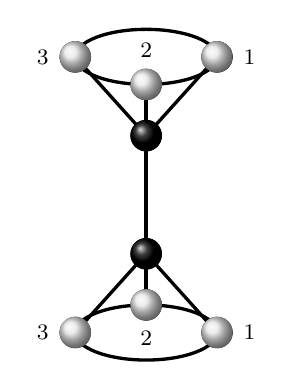
\begin{tikzpicture}[very thick, baseline=(current bounding box), font=\footnotesize]
        \draw (0, 1.5) -- (-0.9, 2.5);
        \draw (0, 1.5) -- (0.9, 2.5);
        \draw (0, 1.5) -- (0, 2.15);
        \draw (0, 2.5) circle [x radius = 0.9, y radius = 0.35];
        
        \draw (0, 0) -- (-0.9, -1);
        \draw (0, 0) -- (0.9, -1);
        \draw (0, 0) -- (0, -0.65);
        \draw (0, -1) circle [x radius = 0.9, y radius = 0.35];
        
        \draw (0, 0) -- (0, 1.5);
        
        \fill[ball color=black] (0, 0) circle [radius = 0.2];
        \fill[ball color=black] (0, 1.5) circle [radius = 0.2];
        
        \fill[ball color=black!10] (-0.9, 2.5) circle [radius = 0.2];
        \fill[ball color=black!10] (0.9, 2.5) circle [radius = 0.2];
        \fill[ball color=black!10] (0, 2.15) circle [radius = 0.2];
        
        \fill[ball color=black!10] (-0.9, -1) circle [radius = 0.2];
        \fill[ball color=black!10] (0.9, -1) circle [radius = 0.2];
        \fill[ball color=black!10] (0, -0.65) circle [radius = 0.2];
        
        \node[right] at (1.1, 2.5) {1};
        \node[above] at (0, 2.35) {2};
        \node[left] at (-1.1, 2.5) {3};
        \node[right] at (1.1, -1) {1};
        \node[below] at (0, -0.85) {2};
        \node[left] at (-1.1, -1) {3};
    \end{tikzpicture}
    \caption{Ethane molecule.}
    \label{fig:ethane molecule}
\end{figure}

\chapter{Permutation Groups}
\section{Symmetric Group}
\begin{dfn}{Permutation}{}
    A \defineindex{permutation}, \(\sigma\), on \(n\) objects is a bijection \(\sigma \colon X \to X\) where \(\abs{X} = n\).
\end{dfn}

Typically, we identify \(X\) as \(\{1, \dotsc, n\}\).

\begin{dfn}{Symmetric Permutation Group}{}
    The \defineindex{symmetric group} on \(n\) objects is the set of all permutations on \(n\) objects with function composition as a group operation.
    This group is denoted \(S_n\).
\end{dfn}

The order of \(S_n\) is \(n!\), since we can choose to permute the first element to any of \(n\) possible options, the second to any of \(n - 1\) options, and so on giving \(n(n - 1) \dotsm 1 = n!\) choices.

\begin{lma}{}{}
    The symmetric group on \(n\) objects is a group.
    \begin{proof}
        Let \(\sigma, \rho \in S_n\).
        Then both of these are bijections on some set \(X\) with \(\abs{X} = n\).
        Their composition is defined by \((\sigma \circ \rho)(x) = \sigma(\rho(x))\) for all \(x \in X\).
        Straight away we see that this is indeed a permutation, since \(\sigma \circ \rho \colon X \to X\) and the inverse is \(\rho^{-1} \circ \sigma^{-1}\), the existence of said inverses in \(S_n\) is guaranteed as \(\sigma \in S_n\) is a bijection and so its inverse exists and is also a bijection.
        This shows that \(S_n\) is closed.
        
        The identity function, \(\mathrm{id}_X \colon X \to X\) defined by \(\mathrm{id}_X(x) = x\) for all \(x \in X\) is a permutation and \(\mathrm{id}_X \circ \sigma = \sigma\) for all \(\sigma \in S_n\).
        As previously discussed \(\sigma\) has the inverse \(\sigma^{-1}\), which is such that \(\sigma\circ \sigma^{-1} = \mathrm{id}_X\).
        Hence, \(S_n\) is a group.
    \end{proof}
\end{lma}

\(S_n\) acts on the set of all tuples \((x_1, \dotsc, x_n)\) where \(x_i \in X\) are distinct in the obvious way, namely by permuting the elements:
\begin{equation}
    \sigma \action (x_1, \dotsc, x_n) = (\sigma(x_1), \dotsc, \sigma(x_n)).
\end{equation}

\begin{dfn}{Cycle}{}
    A \(k\)-\defineindex{cycle} is a way of writing a certain permutation.
    Namely, \(\cycle{a_1, \dotsc, a_k}\) with \(a_i \in X\) is the permutation that sends \(a_1\) to \(a_2\), \(a_2\) to \(a_3\), and so on until \(a_{k-1}\) to \(a_k\) and \(a_k\) to \(a_1\).
    All \(x \in X\) such that \(x \ne a_i\) are left unchanged.
    
    A 2-cycle is also called a \defineindex{transposition}.
    
    The identity is usually written as \(\cycle{}\) when using cycle notation, although we could also write it as a 1-cycle, \(\cycle{a}\) for any \(a \in X\).
    
    Given a \(k\)-cycle \(\cycle{a_1, \dotsc, a_k}\) we can start on any element of this cycle, so this is equivalent to \(\cycle{a_m, \dotsc, a_k, a_1, \dotsc, a_{m-1}}\).
\end{dfn}

\begin{figure}
    \tikzsetnextfilename{cycle}
    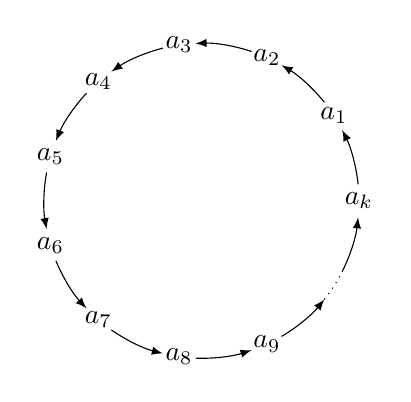
\begin{tikzpicture}
        \foreach \a in {1, ..., 9} {
            \node (a\a) at (360*\a/11:2) {\(a_{\a}\)};
            \draw[->] (360*\a/11+6:2) arc(360*\a/11+6:{360*(\a+1)/11-6}:2);
        }
        \coordinate (a10) at (3600/11:2);
        \draw[dotted] (3600/11-6:2) arc(3600/11-6:3600/11+6:2);
        \draw[->] (3600/11+6:2) arc(3600/11+6:3960/11-6:2);
        \node (al) at (3960/11:2) {\(a_k\)};
        \draw[->] (3960/11+6:2) arc(3960/11+6:4320/11-6:2);
    \end{tikzpicture}
    \caption{The \(k\)-cycle \(\cycle{a_1, \dotsc, a_k}\).}
\end{figure}

\begin{exm}{}{}
    Consider \(S_4\), this contains the 3-cycles \(\cycle{1, 4, 2}\) and \(\cycle{1, 2, 3}\).
    We can work out their product by considering their action on some 4-tuple \((a, b, c, d)\):
    \begin{align}
        \cycle{1, 4, 2}\cycle{1, 2, 3} \action \cycle{a, b, c, d} &= \cycle{1, 4, 2} \action (c, a, b, d)\\
        &= (a, d, b, c)\\
        &= \cycle{2, 3, 4} \action (a, b, c, d),
    \end{align}
    hence, we have \(\cycle{1, 4, 2}\cycle{1, 2, 3} = \cycle{2, 3, 4}\).
\end{exm}

\begin{dfn}{Disjoint Cycles}{}
    Two cycles are disjoint if no element of \(X\) appears in both cycles.
\end{dfn}

\begin{lma}{}{}
    All permutations can be written as a product of disjoint cycles.
    
    \begin{proof}
        We proceed by induction on the size of \(n = \abs{X}\).
        Clearly if \(n = 1\) then the only permutation is the identity, \(\cycle{}\).
        
        Let \(\sigma \in S_n\) and suppose that all cycles in \(S_{n-1}\) can be written as disjoint cycles.
        For simplicity, we will take \(X = \{1, \dotsc, n\}\).
        If \(\sigma(n) = n\) then we can consider \(\sigma\) as a permutation on \(\{1, \dotsc, n - 1\}\) leaving \(n\) fixed, and we are done since this can be written as a product of disjoint cycles.
        If \(\sigma(n) = k \ne n\) then consider the permutation \(\rho = \cycle{n, k} \sigma\).
        We have that \(\rho(n) = \cycle{n, k}\sigma(n) = \cycle{n, k}(k) = n\), here we are treating \(\cycle{n, k}\) as a function, \(\cycle{n, k} \colon \{1, \dotsc, n\} \to \{1, \dotsc, n\}\), defined by \(\cycle{n, k}(n) = k\), \(\cycle{n, k}(k) = n\) and \(\cycle{n, k}(a) = a\) for \(a \ne n, k\).
        So we can think of \(\rho\) as being a permutation on \(\{1, \dotsc, n - 1\}\), and hence can be written as a product of disjoint cycles, \(\rho = \tau_1\dotsm \tau_r\).
        The cycles \(\tau_i\) only contain the numbers \(1, \dotsc, n -1\), and each appears in at most one of these cycles.
        
        Clearly \(\cycle{n, k}\cycle{n, k} = \cycle{}\), and so it follows that
        \(\sigma = \cycle{n, k}\cycle{n, k}\sigma = \cycle{n, k}\tau_1\dotsm \tau_r\).
        If \(k\) doesn't appear in any of the cycles \(\tau_i\) then we are done as this is a product of disjoint cycles.
        Disjoint cycles commute, since by being disjoint they act on different elements of the tuple \((x_1, \dotsc, x_n)\), and so don't interact, meaning the order doesn't matter.
        Using this we are free to assume that the cycle in which \(k\) appears, if it appears, is \(\tau_1\).
        
        We are free to start on any element of the cycle, so we write \(\tau_1 =\cycle{k, a_1, \dotsc, a_m}\).
        We then have
        \begin{equation}
            \cycle{n, k}\tau_1 = \cycle{n, k}\cycle{k, a_1, \dotsc, a_m} = \cycle{n, k, a_1, \dotsc, a_m}.
        \end{equation}
        This follows by considering \(\cycle{n, k}\tau_1(k) = \cycle{n, k}(a_1) = a_1\), \(\cycle{n, k}\tau_1(n) = \cycle{n, k}(n) = k\), \(\cycle{n, k}\tau_1(a_m) = \cycle{n, k}(k) = n\), and \(\cycle{n, k}\tau_1(a_i) = \cycle{n, k}a_{i+1} = a_{i+1}\) for \(i \ne m\).
        It follows then that we can write
        \begin{equation}
            \sigma = \cycle{n, k, a_1, \dotsc, a_m}\tau_2\dotsm \tau_r
        \end{equation}
        which is a product of disjoint cycles.
        
        Hence, by induction we can write any permutation in \(S_n\) as a product of disjoint cycles for all \(n \in \naturals\).
    \end{proof}
\end{lma}

One question that we may reasonably ask is how many \(m\)-cycles are there in \(S_n\) for some fixed \(m \in \{1, \dotsc, n\}\).
If the order of a cycle didn't matter then there would be \(\binom{n}{m}\) \(m\)-cycles in \(S_n\).
However, the order does matter.
Suppose we have chosen our \(m\) terms to appear in the cycle.
We can start with any of them, reducing the number of choices that give distinct cycles by a factor of \(1/m\).
There are then \((m - 1)!\) choices for ordering the \(m - 1\) elements remaining, giving the number of \(m\)-cycles to be
\begin{equation}
    \binom{n}{m} \frac{1}{m} (m - 1)! = \frac{n!}{(n - m)!m!}\frac{1}{m} (m - 1)! = \frac{n!}{(n - m)!}
\end{equation}
where we have used \(m(m - 1)! = m!\).

\begin{thm}{}{thm:transpositions generate Sn}
    The transpositions generate \(S_n\).
    That is, all permutations can be written as a product of 2-cycles.
    
    \begin{proof}
        All elements of \(S_n\) are simply \(k\)-cycles for some \(k \in \{1, \dotsc, n\}\).
        An arbitrary \(k\)-cycle can be written as
        \begin{equation}
            \cycle{a_1, a_2, \dotsc, a_k} = \cycle{a_1, a_k}\cycle{a_1, a_{k-1}} \dotsm \cycle{a_1, a_2}.
        \end{equation}
        To see why this works we consider three cases.
        First, if this acts on some \(a_i\) with \(i \ne 1\), on the left-hand side we clearly see that \(a_i\) maps to \(a_{i + 1}\).
        On the right-hand side \(a_{i}\) commutes with cycles until a cycle with \(a_{i}\) occurs, this cycle will be \(\cycle{a_1, a_i}\), and so \(a_i\) will be sent to \(a_1\).
        The next cycle is then \(\cycle{a_1, a_{i + 1}}\), and hence \(a_1\) maps to \(a_{i + 1}\) which then commutes with all of the remaining cycles.
        Hence, \(a_i\) will map to \(a_{i+1}\).
        
        The second case is when this acts on \(a_1\), in which case the first cycle sends \(a_1\) to \(a_2\), which then commutes with all remaining cycles and so \(a_1\) maps to \(a_2\), which is what we want.
        
        The final case is trivial, it's where this acts on some \(a \ne a_i\) for any \(i\), in which case on both the left and right this element is not changed, and we are finished.
    \end{proof}
\end{thm}

The above theorem is fairly obvious.
It states that we can do any permutation just by swapping two items at a time.
This is demonstrated in \cref{fig:permutation transposition}.

\begin{figure}
    \tikzsetnextfilename{permutation-by-transpositions}
    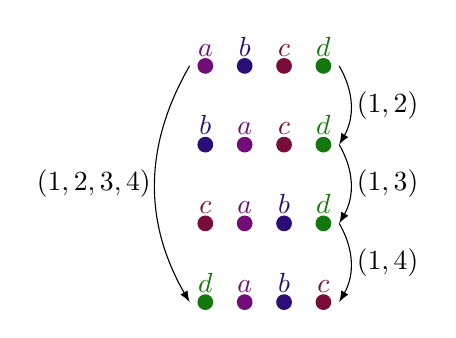
\begin{tikzpicture}
        \fill[highlight] (0, 0) circle [radius = 0.1] node[above] {\(a\)};
        \fill[my blue] (0.5, 0) circle [radius = 0.1] node[above] {\(b\)};
        \fill[my red] (1, 0) circle [radius = 0.1] node[above] {\(c\)};
        \fill[my green] (1.5, 0) circle [radius = 0.1] node[above] {\(d\)};
        
        \begin{scope}[yshift=-1cm]
            \fill[highlight] (0.5, 0) circle [radius = 0.1] node[above] {\(a\)};
            \fill[my blue] (0, 0) circle [radius = 0.1] node[above] {\(b\)};
            \fill[my red] (1, 0) circle [radius = 0.1] node[above] {\(c\)};
            \fill[my green] (1.5, 0) circle [radius = 0.1] node[above] {\(d\)};
        \end{scope}
        
        \begin{scope}[yshift=-2cm]
            \fill[highlight] (0.5, 0) circle [radius = 0.1] node[above] {\(a\)};
            \fill[my blue] (1, 0) circle [radius = 0.1] node[above] {\(b\)};
            \fill[my red] (0, 0) circle [radius = 0.1] node[above] {\(c\)};
            \fill[my green] (1.5, 0) circle [radius = 0.1] node[above] {\(d\)};
        \end{scope}
        
        \begin{scope}[yshift=-3cm]
            \fill[highlight] (0.5, 0) circle [radius = 0.1] node[above] {\(a\)};
            \fill[my blue] (1, 0) circle [radius = 0.1] node[above] {\(b\)};
            \fill[my red] (1.5, 0) circle [radius = 0.1] node[above] {\(c\)};
            \fill[my green] (0, 0) circle [radius = 0.1] node[above] {\(d\)};
        \end{scope}
        
        \draw[->] (1.7, 0) to[bend left] (1.7, -1);
        \node[right] at (1.8, -0.5) {\((1, 2)\)};
        \draw[->] (1.7, -1) to[bend left] (1.7, -2);
        \node[right] at (1.8, -1.5) {\((1, 3)\)};
        \draw[->] (1.7, -2) to[bend left] (1.7, -3);
        \node[right] at (1.8, -2.5) {\((1, 4)\)};
        
        \draw[->] (-0.2, 0) to[bend right] (-0.2, -3);
        \node[left] at (-0.57, -1.5) {\((1, 2, 3, 4)\)};
    \end{tikzpicture}
    \caption[Permutation by transposition.]{The permutation \(\cycle{1, 2, 3, 4}\) acts on \((a, b, c, d)\), which can be done in steps where each step is a transposition.}
    \label{fig:permutation transposition}
\end{figure}

Notice that this theorem implies that the rank of \(S_n\) is at most 
\begin{equation}
    \binom{n}{2} = \frac{n!}{2!(n - 2)!} = \frac{1}{2}n(n - 1),
\end{equation}
although we will see it is less than this.

\begin{lma}{}{lma:transpositions 1 a generate Sn}
    The transpositions, \(\{\cycle{1, 2}, \cycle{1, 3}, \dotsc, \cycle{1, n}\}\), generate \(S_n\).
    \begin{proof}
        Notice that
        \begin{equation}
            \cycle{a_1, a_2} = \cycle{1, a_1} \cycle{1, a_2} \cycle{1, a_1}.
        \end{equation}
        To see this we can consider this acting on \(\cycle{1, \dotsc, a_1, \dotsc, a_2, \dotsc}\):
        \begin{align}
            \cycle{1, a_1}\cycle{1, a_2}\cycle{1, a_1}&\cycle{1, \dotsc, a_1, \dotsc, a_2, \dotsc}\\
            &= \cycle{1, a_1}\cycle{1, a_2}\cycle{a_1, \dotsc, 1, \dotsc, a_2, \dotsc}\\
            &= \cycle{1, a_1}\cycle{a_1, \dotsc, a_2, \dotsc, 1, \dotsc}\\
            &= \cycle{1, \dotsc, a_2, \dotsc, a_1, \dotsc}
        \end{align}
        so the action of \(\cycle{1, a_1}\cycle{1, a_2}\cycle{1, a_1}\) is to swap \(a_1\) and \(a_2\), which is exactly the action of \(\cycle{a_1, a_2}\).
        Using this we can generate any transposition from transpositions of the form \(\cycle{1, a}\).
        Therefore, by \cref{thm:transpositions generate Sn} transpositions of this form generate \(S_n\).
    \end{proof}
\end{lma}

Notice that this theorem implies that the rank of \(S_n\) is at most \(n\), for \(n > 3\) this is an improvement on our previous bound.

\begin{lma}{}{lma:transpositions a-1 a generate Sn}
    The transpositions, \(\{\cycle{1, 2}, \cycle{2, 3}, \dotsc, \cycle{n - 1, n}\}\), generate \(S_n\).
    \begin{proof}
        Notice that
        \begin{equation}
            \cycle{1, k} = g\cycle{1, 2}g^{-1}
        \end{equation}
        where \(g = \cycle{k - 1, k}\dotsm \cycle{3, 4}\cycle{2, 3}\).
        To see this first notice that \(g^{-1} = \cycle{2, 3}\cycle{3, 4}\dotsm \cycle[\enspace]{k - 1, k}\).
        Then notice that the action of \(g^{-1}\) is to exchange \(k - 1\) and \(k\), then swap \(k\) and \(k - 2\), and then \(k\) and \(k - 3\), and so on until \(k\) and \(2\) have been swapped.
        Then \(\cycle{1, 2}\) swaps \(k\) and 1.
        We then use \(g\) to swap \(2\) and \(3\) back, then \(3\) and \(4\), and so on until we swap \(k - 2\) and \(k - 1\) back to their original positions.
        The result is that \(1\) and \(k\) swap, which is exactly what \(\cycle{1, k}\) does.
        
        Using this we can generate any transposition of the form \(\cycle{1, a}\) from transpositions of the form \(\cycle[\enspace]{k - 1, k}\), and so by \cref{lma:transpositions 1 a generate Sn} these transpositions generate \(S_n\).
    \end{proof}
\end{lma}

We can think of this proof as consisting of a basis change from the \(\cycle{1, a}\) transpositions case, and similarly for the next proof.

\begin{lma}{}{lma:12 and 12...n generate Sn}
    The cycles, \(\{\cycle{1, 2}, \cycle{1, 2, \dotsc, n}\}\), generate \(S_n\).
    \begin{proof}
        Notice that
        \begin{equation}
            \cycle[\enspace]{k, k + 1} = g\cycle{1, 2}g^{-1}
        \end{equation}
        where \(g = \cycle{1, 2, \dotsc, n}^{k-1}\).
        To see this first notice that \(g^{-1} = \cycle{n, \dotsc, 2, 1}^{k - 1}\).
        The action of \(g^{-1}\) is then to cycle backwards through the elements \(k - 1\) times.
        The result is that \(k\) and \(k + 1\) end up in the first two positions.
        These are then swapped by \(1, 2\).
        Then \(g\) cycles forwards through the elements \(k - 1\) times, and we end up with the same tuple but with \(k\) and \(k + 1\) swapped, which is exactly what \(\cycle[\enspace]{k, k + 1}\) does.
        
        Using this we can generate any transposition of the form \(\cycle{k, k + 1}\), and so by \cref{lma:transpositions a-1 a generate Sn} these two cycles generate \(S_n\).
    \end{proof}
\end{lma}

\begin{crl}{}{}
    The rank of \(S_n\) is 2.
    \begin{proof}
        \(S_n\) is generated by \(\{\cycle{1, 2}, \cycle{1, \dotsc, n}\}\) by \cref{lma:12 and 12...n generate Sn}, so \(S_n\) is of rank 2.
    \end{proof}
\end{crl}

\section{Alternating Group}
We have seen that any permutation can be written as a product of transpositions by \cref{thm:transpositions generate Sn}.
It turns out that the number of transpositions it takes to write any given permutation is unambiguously even or odd.
We then term the permutation as even or odd based on the parity of the number of transpositions it takes to write it.
This is the obvious definition of even and odd permutations, but it isn't that easy to work with, so we use an equivalent, but easier to work with, definition.

\begin{dfn}{Sign of a Permutation}{dfn:sign of a permutation}
    Let \(S_n\) be the symmetric group on \(n\) letters.
    Define the \defineindex{Vandermonde polynomial} to be
    \begin{align}
        P(x_1, \dotsc, x_n) &\hphantom{:}= P(\vv{x})\\
        &\coloneqq (x_1 - x_2)(x_1 - x_2) \dotsm (x_1 - x_n)\\
        &\qquad\cdot(x_2 - x_3) \dotsm (x_2 - x_n) \dotsm (x_{n - 1} - x_n)\\
        &\hphantom{:}= \prod_{\mathclap{\substack{i, j \in \{1, \dotsc, n\}\\ i < j}}} (x_i - x_j).
    \end{align}
    This polynomial is such that exchanging any two variables, \(x_i\) and \(x_j\), results in the sign of the polynomial changing.
    
    Define \(X\) to be the set of all permutations of \((x_1, \dotsc, x_n)\).
    We can define a group action, \(\varphi \colon S_n \times X \to X\), in the usual way as \(S_n\) acting on \(\vv{x} \in X\) by permutation.
    
    Now define \(\sgn \colon S_n \to \{\pm 1\}\) by \(\sgn(\sigma) = P(\sigma\action \vv{x})/\abs{P(\vv{\vv{x}})}\).
    Then if \(\sgn(\sigma) = 1\) we say \(\sigma\) is an \defineindex{even permutation} and if \(\sgn(\sigma) = -1\) we say that \(\sigma\) is an \defineindex{odd permutation}.
    This agrees with the \enquote{parity of the number of transpositions} definition since each transposition swaps two variables and so an even number of transpositions corresponds to an even number of swaps and hence no overall sign change, similarly an odd number of transpositions will result in a sign change.
\end{dfn}

\begin{dfn}{Alternating Group}{}
    The \defineindex{alternating group}, \(A_n\)\index{An@\(A_n\), alternating group}, is the group of all even permutations on \(n\) letters.
\end{dfn}

\begin{thm}{}{}
    The alternating group, \(A_n\), is a normal subgroup of the symmetric group, \(S_n\).
    \begin{proof}
        We claim that \(\psi \colon S_n \to \integers_2\) as defined in \cref{dfn:sign of a permutation} is a group homomorphism.
        First notice that \(\sgn(\sigma\rho) = P(\sigma\rho\action \vv{x})/\abs{P(\vv{x})}\).
        Now consider \(\sgn(\sigma)\sgn(\rho) = P(\sigma\action\vv{x})P(\rho\action\vv{x})/\abs{P(\vv{x})}^2\).
        Hence, \(\sgn(\sigma)\sgn(\rho) = 1\)  if \(\sigma\) and \(\rho\) have the same parity and \(\sgn(\sigma)\sgn(\rho) = -1\) if \(\sigma\) and \(\rho\) have opposite parities.
        Suppose \(\sigma = s_1\dotsm s_k\) and \(\rho = r_1\dotsm r_m\) where \(s_i\) and \(r_i\) are transpositions.
        Then \(\sigma\rho = s_1\dotsm s_k r_1 \dotsm r_m\) is a product of \(k + m\) transpositions.
        This is even if \(k\) and \(m\) are both even, or both odd, and odd if \(k\) and \(m\) have opposite parities.
        Therefore, \(\sgn(\sigma\rho) = P(\sigma\rho\action\vv{x})/\abs{P(\vv{x})}\) is 1 if \(\sigma\) and \(\rho\) are the same parity and \(-1\) if they are opposite parities.
        Hence, \(\sgn\) is a homomorphism.
        
        The kernel of \(\sgn\) is \(A_n\), since even permutations map to \(1\) by definition.
        Hence, by \cref{thm:first isomorphism} \(A_n\) is a normal subgroup of \(S_n\).
    \end{proof}
\end{thm}

\begin{lma}{}{}
    The three-cycles generate \(A_n\).
    \begin{proof}
        Notice that \(\cycle{1, a_1}\cycle{1, a_2} = \cycle{1, a_1, a_2}\).
        Since transpositions of the form \(\cycle{1, a}\) generate \(S_n\) and \(A_n\) consists of all permutations which can be written as a product of an even number of transpositions we can always pair up transpositions like this to write elements of \(A_n\) as a product of three cycles.
        Hence, the three-cycles generate \(A_n\).
    \end{proof}
\end{lma}

Notice that the order of \(A_n\) is \(\abs{A_n} = \abs{S_n}/\abs{\integers_2} = n!/2\).

\chapter{Applications}
\section{Platonic Solids}
\begin{dfn}{Platonic Solid}{}
    A \defineindex{Platonic solid} is a regular convex polyhedron.
\end{dfn}

There are five Platonic solids, the tetrahedron, cube, octahedron, dodecahedron, and icosahedron.
These have 4, 6, 8, 12, and 20 faces, respectively, and are formed from equilateral triangles, squares, equilateral triangles, regular pentagons, and equilateral triangles, respectively.

Each Platonic solid has an associated symmetry group, which acts on the solid leaving it invariant.
These symmetry groups are all permutation groups, both symmetric and alternating.
We can think of them as acting by permuting the vertices of the solid.
The reason why the full symmetry group is not necessarily all of \(S_n\) is because certain permutations aren't allowed, for example, if two vertices are connected by an edge then this must be the case after permuting vertices.

\begin{table}
    \caption{The Platonic solids, along with the number of faces, \(F\), vertices, \(V\), and edges, \(E\), which are related by Euler's formula, \(V - E + F = 2\), the regular polygons that make up their faces, and their symmetry groups. Notice that duals have the same symmetry groups, the same number of edges and that the number of faces and vertices are swapped.}
    \begin{tabular}{lccclc}\toprule
        Sold & \(F\) & \(V\) & \(E\) & Polygon & Symmetry Group \\ \midrule
        Tetrahedron & 4 & 4 & 6 & Triangle & \(A_4\)\\
        Cube & 6 & 8 & 12 & Square & \(S_4\)\\
        Octahedron & 8 & 6 & 12 & Triangle & \(S_4\)\\
        Dodecahedron & 12 & 20 & 30 & Pentagon & \(A_5\)\\
        Icosahedron & 20 & 12 & 30 & Triangle & \(A_5\)\\\bottomrule
    \end{tabular}
\end{table}

The dual of a Platonic solid is the Platonic solid you get if you swap the vertices and faces, that is if you join the centre of two faces if they have a common edge.
This is demonstrated in \cref{fig:dual} for the cube and octahedron.
The tetrahedron is its own dual, the cube and octahedron are dual and the dodecahedron and icosahedron are dual.
Duals have the same symmetry group.

\begin{figure}
    \tikzsetnextfilename{cube-octahedron-dual}
    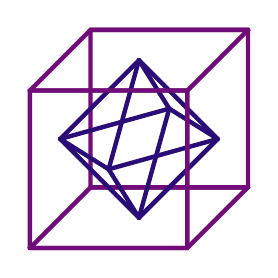
\begin{tikzpicture}[highlight, ultra thick, rounded corners=0.01, text=black]
        \pgfmathsetmacro{\r}{2}
        \coordinate (A) at (0, 0, 0);
        \coordinate (B) at (\r, 0, 0);
        \coordinate (C) at (\r, 0, \r);
        \coordinate (D) at (0, 0, \r);
        \coordinate (E) at (0, \r, 0);
        \coordinate (F) at (\r, \r, 0);
        \coordinate (G) at (\r, \r, \r);
        \coordinate (H) at (0, \r, \r);
        \draw (A) -- (B) -- (C) -- (D) -- cycle;
        \draw (E) -- (F) -- (G) -- (H) -- cycle;
        \draw (A) -- (E) -- (F) -- (B) -- cycle;
        \coordinate (a) at (\r/2, 0, \r/2);
        \coordinate (b) at (0, \r/2, \r/2);
        \coordinate (c) at (\r/2, \r/2, 0);
        \coordinate (d) at (\r, \r/2, \r/2);
        \coordinate (e) at (\r/2, \r/2, \r);
        \coordinate (f) at (\r/2, \r, \r/2);
        \draw[my blue] (b) -- (c) -- (d) -- (e) -- cycle;
        \draw[my blue] (b) -- (a) -- (c);
        \draw[my blue] (d) -- (a) -- (e);
        \draw[my blue] (b) -- (f) -- (c);
        \draw[my blue] (d) -- (f) -- (e);
        \draw (C) -- (G) -- (H) -- (D) -- cycle;
    \end{tikzpicture}
    \caption{The octahedron is the dual of the cube.}
    \label{fig:dual}
\end{figure}

Consider the tetrahedron, with the symmetry group \(A_4\).
This group is of order \(4! / 2 = 12\).
\(A_4\) is generated by two symmetries shown in \cref{fig:tetrahedron symmetries}.

\begin{figure}
    \tikzsetnextfilename{tetrahedron-symmetries}
    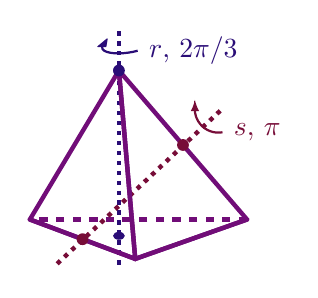
\begin{tikzpicture}[highlight, ultra thick, rounded corners=0.01]
        \pgfmathsetmacro{\r}{1.3}
        \coordinate (A) at (0, 0, \r);
        \coordinate (B) at ({\r*sqrt(2)/2}, 0, 0);
        \coordinate (C) at ({-\r*sqrt(2)}, 0, 0);
        \coordinate (D) at (0, \r*2, {\r*sqrt(2)});
        \draw[dashed] (B) -- (C);
        \draw[my blue, dotted] (0, \r*2+0.5, {\r*sqrt(2)}) -- ++ (0, -3, 0);
        \draw[my red, dotted] (-1.3, -0.37, 0.5) -- (0.8, 1.6, 0.5);
        \draw (B) -- (A) -- (C);
        \draw (A) -- (B) -- (D) -- cycle;
        \draw (C) -- (D) -- (A) -- cycle;
        \fill[my blue] (D) circle [radius=0.075];
        \fill[my blue] (0, 0.5, {\r*sqrt(2)}) circle [x radius=0.075, y radius=0.05];
        \fill[my red] ($(A)!0.5!(C)$) circle [radius=0.075];
        \fill[my red] ($(D)!0.5!(B)$) circle [radius=0.075];
        
        
        \draw[my blue, canvas is xz plane at y=3, thick] ({sqrt(0.15)}, {\r*sqrt(2) + sqrt(0.15)}) arc(45:165:0.3);
        \draw[my blue, thin, canvas is xz plane at y=3, fill=my blue] (-0.15, {\r*sqrt(2)}) -- ++ (-0.02, 0.25) -- ++ (0.1, 0) -- cycle;
        \node[my blue, right] at ({sqrt(0.15)}, 3, {\r*sqrt(2) + sqrt(0.15)}) {\(r\), \(2\pi/3\)};
        
        \draw[my red, thick] (0.8, 1.3, 0.5) arc(100:0:-0.3);
        \draw[my red, thin, ->] (0.45, 1.7, 0.5) -- ++ (0, 0.01, 0);
        \node[my red, right] at (0.8, 1.3, 0.5) {\(s\), \(\pi\)};
    \end{tikzpicture}
    \caption{Two possible symmetries of the tetrahedron}
    \label{fig:tetrahedron symmetries}
\end{figure}

For the case of the cube we can view \(S_4\) as acting by permuting the diagonals of the cube.

\section{Molecules}
For a molecule to have a permanent electric dipole it must necessarily have some level of asymmetry, since a spherically symmetric molecule cannot have a preferred direction for a dipole to lie along.
For example, water, has a permanent dipole, and it has as a symmetry  group \(\integers_2\), as shown in \cref{fig:water}.

\begin{figure}
    \tikzsetnextfilename{water}
    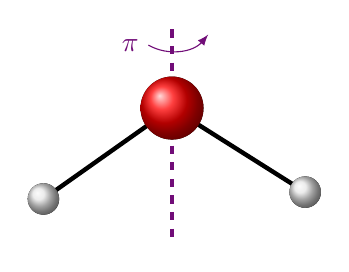
\begin{tikzpicture}
        \draw[highlight, dashed, very thick] (0, 1) -- (0, -1.7);
        \draw[highlight, ->] (-0.3, 0.8) arc(60:140:-0.6);
        \node[left, highlight] at (-0.3, 0.8) {\(\pi\)};
        \draw[ultra thick] (-32.25:2) -- (0, 0) -- (215.25:2);
        \fill[ball color=black!10] (-32.25:2) circle [radius=0.2];
        \fill[ball color=black!10] (215.25:2) circle [radius=0.2];
        \fill[ball color=red] (0, 0) circle [radius=0.4];
    \end{tikzpicture}
    \caption{Water, with symmetry group \(\integers_2\), has a permanent dipole.}
    \label{fig:water}
\end{figure}

Any molecule with symmetry group \(\integers_n\) with \(n \in \{2, 3, \dotsc\}\) cannot have a permanent electric dipole perpendicular to the symmetry axis.
For example, water's electric dipole is aligned with its symmetry axis.

Consider again the case of ethene, \ce{C2H6}, shown in \cref{fig:ethane molecule}.
This has symmetry group \(D_3 \isomorphic \integers_2 \ltimes \integers_3\).
With \(\integers_3\) corresponding to rotations by \(2\pi/3\) about the carbon-carbon bond and \(\integers_2\) corresponding to either inversion about the middle of the carbon-carbon bond or rotations about the perpendicular bisector to the carbon-carbon bond, depending on whether the molecule is eclipsed or staggered.
Either way \ce{C2H6} cannot have a permanent dipole since the two axis of symmetry are orthogonal.
For example, suppose there was an electric dipole aligned with the \(\integers_3\) symmetry axis.
Then the action of \(\integers_2\) would be to reverse the dipole, and hence this isn't a valid permanent dipole.

It can be shown that only molecules with a cyclic symmetry group, \(\integers_n\), can have permanent dipoles.

Another example of symmetry applications to molecules is chirality.
A molecule is chiral if it is different from its mirror image.
Another way of saying this is that a molecule is chiral if it does not admit an improper rotation axis, an improper rotation being a rotation followed by an inversion.

\begin{figure}
    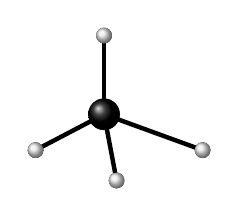
\begin{tikzpicture}[baseline=(current bounding box)]
        \pgfmathsetmacro{\r}{1}
        \coordinate (A) at (0, 0, \r);
        \coordinate (B) at ({\r*sqrt(2)/2}, 0, 0);
        \coordinate (C) at ({-\r*sqrt(2)}, 0, 0);
        \coordinate (D) at (0, \r*2, {\r*sqrt(2)});
        \coordinate (E) at ($(D) - (0, 1, 0)$);
        \draw[ultra thick] (A) -- (E);
        \draw[ultra thick] (B) -- (E);
        \draw[ultra thick] (C) -- (E);
        \draw[ultra thick] (D) -- (E);
        \fill[ball color=black] (E) circle[radius=0.2];
        \fill[ball color=black!10] (A) circle[radius=0.1];
        \fill[ball color=black!10] (B) circle[radius=0.1];
        \fill[ball color=black!10] (C) circle[radius=0.1];
        \fill[ball color=black!10] (D) circle[radius=0.1];
    \end{tikzpicture}
    \hspace{1cm}
    \tetrahedron{ball color=black!10}{ball color=black!10}{ball color=black!10}{ball color=black!10}
    \caption[Methane is tetragonal.]{Methane is a tetragonal molecule, meaning that it has a central atom, here carbon, and four atoms arranged around it making the points of a tetrahedron.}
    \label{fig:methane}
\end{figure}

A tetragonal molecule is one where there is a centre atom with four atoms around it at the points of a tetrahedron, such as methane, \ce{CH4}, shown in \cref{fig:methane}.
An example of a tetragonal molecule which is achiral is \ce{CCl2BrI}, this is shown here:
\begin{equation}
    \tetrahedron{ball color=my red}{ball color=my blue}{ball color=my green}{ball color=my green} \xrightarrow{\text{Inversion}}
    \invertedtetrahedron{ball color=my red}{ball color=my blue}{ball color=my green}{ball color=my green} \xrightarrow{\text{Rotation}}
    \tetrahedron{ball color=my red}{ball color=my blue}{ball color=my green}{ball color=my green}
\end{equation}
On the other hand \ce{CFClBrI} is chiral, this is shown here:
\begin{equation}
    \tetrahedron{ball color=my red}{ball color=my blue}{ball color=my green}{ball color=my yellow} \xrightarrow{\text{Inversion}}
    \invertedtetrahedron{ball color=my red}{ball color=my blue}{ball color=my green}{ball color=my yellow} \xrightarrow{\text{Rotation}}
    \tetrahedron{ball color=my red}{ball color=my green}{ball color=my blue}{ball color=my yellow}
\end{equation}
Notice that the green and blue are swapped after the inversion and rotation.
    \part{Representation Theory}
\chapter{Basics of Representation Theory}\label{chap:basics of representation theory}
\begin{rmk}
    Material in this section applies both to finite groups and compact
    groups.
    We won't worry too much about what it means for a group to be compact,
    we just note that the Lie groups \(\unitary(1) \isomorphic
    \specialOrthogonal(2)\) and \(\specialOrthogonal(3) \isomorphic
    \specialUnitary(2) / \integers_2\) are compact.
    More generally \(\orthogonal(n)\), \(\specialOrthogonal(n)\),
    \(\Spin(n)\), \(\unitary(n)\), and \(\specialUnitary(n)\) are compact.
\end{rmk}

\section{Representation Definition}
There are two essentially equivalent definitions of a representation:
\begin{dfn}{Representation}{}
    A \defineindex{representation} of a group, \(G\), is a group action of
    \(G\) on a linear space, \(V\).
    That is \(\varphi \colon G \times V \to V\) is a representation if it is
    a group action.
    
    A \defineindex{representation} of a group, \(G\), is a homomorphism with
    the automorphism group of a linear space.
    That is \(\rho \colon G \to \generalLinear(V)\) is a representation if
    it is a homomorphism.
\end{dfn}
The equivalence of these two definitions is simple, if \(\varphi(g, \vv{v})
= g \action \vv{v} = \rho(g)\vv{v}\) for all \(g \in G\) and \(\vv{v} \in V\)
then \(\varphi\) and \(\rho\) are the same representation in the two slightly
different definitions.

When the homomorphism is clear it is common to refer to \(V\) as the
representation, rather than \(\rho\).

Representation theory gives us a way to do concrete calculations in a group.
We have implicitly been using representation theory already, for example we
have used \(\integers_n = \{\e^{2i\pi m/n} \mid m = 0, \dotsc, n - 1\}\) as
\emph{the} cyclic group of order \(n\).
Strictly this is actually a representation of a more general cyclic group,
defined by \(\presentation{g}{g^n = e}\).
The linear space in question is \(\complex\), and \(\generalLinear(\complex)
= \complex\setminus\{0\}\).
The group action is rotation by \(2\pi m/n\).

Representation theory is particularly useful because we have developed a lot
of tools for dealing with computations in linear spaces since they are common in
other areas of maths and physics.
Representation theory allows us to use these to work with groups.

\begin{app}{}{}
    When we solve the quantum harmonic oscillator we can do so in different
    linear spaces, such position space, \(\ket{x}\), momentum space, \(\ket{p}\), or
    number-of-particles space, \(\ket{n}\).
    Each one of these corresponds to studying the same underlying physics on
    a different linear space, which we can think of as being different
    representations.
    
    If a system has a certain symmetry described by a group, \(G\), then
    this is expressed in the mathematics by \(G\) acting on the Hilbert space of
    states, which is to say as a representation of \(G\) on the Hilbert space of
    states.
\end{app}

If the relevant linear space is finite dimensional, say \(\dim V = n\) then
we can associate \(\generalLinear(V)\) with \(\generalLinear(n, \field)\), the
group of \(n \times n\) matrices with entries in \(\field\), and so we can
associate \(\rho(g)\) with a matrix.

\section{Pedestrian Approach}
\begin{rmk}
    In this section we will get an idea of how representation can be used
    without being too worried about precise definitions.
\end{rmk}

Consider \(S_3\).
By \cref{lma:transpositions 1 a generate Sn} \(\{\cycle{1, 2}, \cycle{1,
    3}\}\) generates \(S_n\), so we can define a representation by how it maps these
two elements to the linear space.
Inspired by \(S_3\) as a permutation group we look for a representation that
conserves this permuting ability.
In particular the obvious choice of 3 things to act on in a linear space are
the 3 basis vectors of a 3-dimensional space, such as \(\reals^3\).
We use the standard basis, \(\ve{1} = (1, 0, 0)^\trans\), \(\ve{2} = (0, 1,
0)^\trans\), and \(\ve{3} = (0, 0, 1)^\trans\).
We can easily construct matrices that permute these, for example we want
\(\rho(\cycle{1, 2})\ve{1} = \ve{2}\), \(\rho(\cycle{1, 2})\ve{2} = \ve{2}\) and
\(\rho(\cycle{1, 2})\ve{3} = \ve{3}\).
This fully determines the matrix \(\rho(\cycle{1, 2})\):
\begin{equation}
    \rho(\cycle{1, 2}) = 
    \begin{pmatrix}
        0 & 1 & 0\\
        1 & 0 & 0\\
        0 & 0 & 1
    \end{pmatrix}
    .
\end{equation}
Similarly, we have
\begin{equation}
    \rho(\cycle{1, 3}) = 
    \begin{pmatrix}
        0 & 0 & 1\\
        0 & 1 & 0\\
        1 & 0 & 0
    \end{pmatrix}
    .
\end{equation}
This is called the \defineindex{permutation representation} of \(S_3\), and
can easily be generalised to \(S_n\).

At this point there are a few questions we should consider.
First, are there any other representations?
The answer to this is yes, and we'll see some later.
The second is can we find a simpler representation, for some sense of
simpler.
The answer is again yes.
In particular notice that \(\vv{v} = (1, 1, 1)^{\trans}\) is a common
eigenvector for both of these matrices, and hence there is an invariant
subspace, \(\spn\{\vv{v}\}\), which is unchanged by this representation.
It can be shown that this allows us to perform a basis change and write
these matrices in block diagonal form.
We can then define a new representation, \(\rho'\), in this block diagonal
basis such that
\begin{equation}
    \rho'(\cycle{1, 2}) = 
    \begin{pmatrix}
        1 & 0 & 0\\
        0 & a_{11} & a_{12}\\
        0 & a_{21} & a_{22}
    \end{pmatrix}
    ,\qqand \rho'(\cycle{1, 3}) = 
    \begin{pmatrix}
        1 & 0 & 0\\
        0 & b_{11} & b_{12}\\
        0 & b_{21} & b_{22}
    \end{pmatrix}
    .
\end{equation}
This is simpler because it is fully determined by the \(2\times 2\) block
matrices on the diagonal.
We say that the permutation representation is reducible.

\section{Basic Definitions}
\begin{dfn}{Faithful}{}
    If \(\rho \colon G \to \generalLinear(V)\) is a representation of \(G\)
    then we say \(\rho\) is \define{faithful}\index{faithful representation} if it
    is injective, that is \(\rho(g) = \rho(g')\) implies \(g = g'\).
    If this is not the case then we say \(\rho\) is
    \define{unfaithful}\index{unfaithful representation}.
\end{dfn}

The permutation representation of \(S_3\) is faithful.

\begin{dfn}{Trivial Representation}{}
    Let \(\rho\colon G \to \generalLinear(V)\) be defined by \(\rho(g) = \rho(e) = \ident_V\), where
    \(\ident_V\) is the identity in \(\generalLinear(V)\) and \(V\) is an
    \emph{arbitrary vector space}.
    We say that \(\rho\) is \emph{A} \defineindex{trivial representation}.
    
    \emph{The} \define{trivial representation} is \(\rho\colon G \to
    \generalLinear(V)\) defined by \(\rho(g) = \rho(e) = \ident_V\), where
    \(\ident_V\) is the identity in \(\generalLinear(V)\) and \(V\) is a
    \emph{one-dimensional vector space}.
\end{dfn}

A trivial representation is maximally unfaithful since all elements map to
the same operator.

\begin{dfn}{Unitary Representation}{}
    If \(\rho \colon G \to \unitary(V)\) is a homomorphism then we say that
    \(\rho\) is a \defineindex{unitary representation}.
    That is a unitary representation is one in which \(\rho(g)\) is a
    unitary operator for all \(g \in G\).
\end{dfn}

We have been working with a unitary representation of \(\integers_n\) as
\(\{\e^{2i\pi m/n} \mid m = 0, \dotsc, n - 1\}\).

\begin{dfn}{Equivalence of Representations}{}
    If \(\rho\) and \(\rho'\) are representations of \(G\) on \(V\) we say
    that \(\rho\) and \(\rho'\) are \define{equivalent}\index{equivalence of
        representations} if they are represented by a \defineindex{similarity
        transform}, that is \(\rho(g) = S\rho'(g)S^{-1}\) for some \(S \in
    \generalLinear(V)\).
    Notice that \(S\) must be the same for all \(g \in G\).
\end{dfn}

As the name suggests the equivalence of representations, \(\sim\), is an
equivalence relation.
Clearly \(\rho \sim \rho\) since \(\rho(g) = \ident_V\rho(g)\ident_V^{-1}\).
Also, if \(\rho \sim \rho'\) then \(\rho(g) = S\rho'(g)S^{-1}\) for some \(S
\in \generalLinear(V)\), and so \(\rho'(g) = S^{-1}\rho(g)S\), identifying \(S =
(S^{-1})^{-1}\) and knowing that if \(S \in \generalLinear(V)\) we also have
\(S^{-1} \in \generalLinear(V)\) we see that \(\rho' \sim \rho\).
Finally, if \(\rho \sim \rho'\) and \(\rho' \sim \rho''\) there exists \(S,
T \in \generalLinear(V)\) such that \(\rho(g) = S\rho'(g)S^{-1}\) and \(\rho'(g)
= T\rho''(g)T^{-1}\), and hence \(\rho(g) = ST\rho''(g)T^{-1}S^{-1} =
(ST)\rho(g)(ST)^{-1}\) and since \(S, T \in \generalLinear(V)\) it follows that
\(ST \in \generalLinear(V)\), and hence \(\rho \sim \rho''\).

\begin{dfn}{Invariant Subspace}{}
    Let \(\rho \colon G \to \generalLinear(V)\) be a representation of the
    group \(G\) on the linear space \(V\).
    Let \(W\) be a subspace of \(V\).
    Then we call \(W\) an \defineindex{invariant subspace} if
    \(\rho(g)\vv{w} \in W\) for all \(g \in G\) and \(\vv{w} \in W\).
    
    Using the group-action definition of a representation \(W\) is an
    invariant subspace if \(\Orb(\vv{w}) \subseteq W\) for all \(\vv{w} \in W\).
\end{dfn}

A trivial representation, \(\rho(g) = \ident_V\), has \(V\) as an invariant
subspace.
Our earlier example of \(S_3\) in the permutation representation has
\(\spn\{(1, 1, 1)^\trans\}\) as an invariant subspace.
All representations leave the trivial subspace, \(\{\vv{0}\}\), invariant.

\begin{dfn}{Irreducible}{}
    We call a representation \define{irreducible}\index{irreducible
        representation} if it has no invariant subspaces, apart from the trivial
    zero-dimensional subspace, \(\{\vv{0}\}\).
    If a representation can be written in block diagonal form then it is
    \define{reducible}\index{reducible representation}
\end{dfn}

It is common to shorten \enquote{irreducible representation} to
\define{irrep}\index{irrep|see{irreducible representation}}.

For finite groups and continuous compact groups the reducible
representations can be written as a direct sum of irreducible representations.
For this reason we often care only about irreducible representations.

The permutation representation of \(S_3\) is reducible.

\begin{lma}{}{}
    If a representation has invariant subspaces then we can write it in
    block diagonal form.
\end{lma}

\begin{dfn}{Real and Complex Representations}{}
    A representation, \(\rho \colon G \to \generalLinear(V)\), is
    \define{real}\index{real representation} if either \(V\) is a real vector space
    or the representation is equivalent to a representation which can be thought of
    as acting on a real vector space by reducing the field of scalars to \(\reals\).
    Alternatively \(\rho\) is equivalent to \(\rho^*\).
    
    A \defineindex{complex representation} is a representation, \(\rho
    \colon G \to \generalLinear(V)\), where \(\rho\) is not equivalent to
    \(\rho^*\).
\end{dfn}

We will refine this notion later to include pseudo-real representations.

The permutation representation of \(S_3\) is real, and hence so is
\(\rho'\), even though it is possible that \(a_{ij}\) and/or \(b_{ij}\) are not
real, since \(\rho\) and \(\rho'\) are equivalent.

\begin{app}{}{}
    Unitary representations are important in quantum physics.
    They are the natural language to describe symmetries on the Hilbert
    space of states since they preserve the inner product, and hence the probability
    of being in a given state.
    
    Further there is a certain view from which particles \emph{are}
    irreducible representations of the Poincar\'e group, \(\reals^{1, 3} \ltimes
    \orthogonal(1, 3)\).
    We then associate complex representations with charged particles and
    real representations with neutral particles.
\end{app}

\section{Some Theorems}
\begin{thm}{Maschke's Theorem}{thm:maschke's theorem}\index{Maschke's
        theorem}
    Any representation of a finite group is equivalent to a unitary
    representation.
    
    \begin{proof}
        Let \(G\) be a finite group, \(V\) a vector space, and \(\rho\colon
        G \to \generalLinear(V)\) a representation.
        Let \(\innerprod{-}{-}\) be an inner product on \(G\).
        The statement of the theorem is equivalent to stating that we can
        define a new inner product on \(V\) such that this inner product is invariant
        under the action of this representation.
        This works since the two inner products will be related by a change
        of basis, and hence this new inner product can be viewed as the old inner
        product after a similarity transform.
        
        The inner product that we define is \(\innerprod{-}{-}_G\), it is
        defined for \(x, y \in V\) as
        \begin{equation}
            \innerprod{x}{y}_G \coloneqq \frac{1}{\abs{G}} \sum_{g \in G}
            \innerprod{\rho(g)x}{\rho(g)y}.
        \end{equation}
        We can think of this inner product being defined by acting on the
        old inner product with the representation and then averaging over \(G\).
        
        We need to show that \(\innerprod{-}{-}_G\) is an inner product and
        that it is invariant with respect to the representation.
        By definition \(\rho(g)x, \rho(g)y \in V\) and so
        \(\innerprod{\rho(g)x}{\rho(g)y}\) is positive definite.
        This carries through the sum and so \(\innerprod{x}{y}_G\) is
        positive definite.
        Linearity and conjugate symmetry of \(\innerprod{-}{-}_G\) similarly
        follows from these same properties for \(\innerprod{-}{-}\) without any
        complications since \(G\) is finite.
        
        Now consider what happens when we first act on \(V\) with
        \(\rho(g')\) for some \(g' \in G\).
        Using the fact that \(\rho\) is a homomorphism we then have
        \begin{align}
            \innerprod{\rho(g')x}{\rho(g')y}_G &= \frac{1}{\abs{G}} \sum_{g
                \in G} \innerprod{\rho(g)\rho(g')x}{\rho(g)\rho(g')y}\\
            &= \sum_{g\in G} \innerprod{\rho(gg')x}{\rho(gg')y}\\
            &= \sum_{g''\in G} \innerprod{\rho(g'')x}{\rho(g'')y}\\
            &= \innerprod{x}{y}_G.
        \end{align}
        In the penultimate step we have used the fact that as \(g\) takes on
        all values in \(G\) \(gg'\) necessarily also takes on all values in \(G\).
        This is due to the fact that in a Cayley table each column must
        contain every element of \(G\) exactly once.
        Hence, summing over \(g\) with factors of \(gg'\) is the same as
        summing over \(g'' = gg'\), only the order of the terms changes and since the
        inner product gives an element of the base field this sum is commutative.
        
        Finally, we remark that 
        \begin{equation}
            \innerprod{x}{y}_G = \innerprod{\rho(g')x}{\rho(g')y}_G =
            \innerprod{\rho(g')^\hermit \rho(g') x}{y}_G
        \end{equation}
        using the property of inner products that \(\innerprod{x}{Ay} =
        \innerprod{A^\hermit x}{y}\) for any inner product, \(\innerprod{-}{-}\), and
        operator \(A\).
        Hence, we can identify that \(\rho(g')^\hermit \rho(g') = \ident\),
        and so \(\rho\) is a unitary representation.
    \end{proof}
\end{thm}

It turns out that being irreducible is an incredibly strong requirement, so
much so that it doesn't really leave much wiggle room, as the next theorem
shows.
Schur's lemma states that there is no room for non-trivial homomorphisms
between irreducible representations.

\begin{thm}{Schur's Lemma}{thm:schurs lemma}\index{Schur's lemma}
    Let \(\rho\colon G \to \generalLinear(V)\) and \(\rho\colon G \to
    \generalLinear(V')\) be irreducible representations of the group \(G\) on some
    finite dimensional vector spaces \(V\) and \(V'\).
    Let \(T \colon V \to V'\) be a linear map satisfying \(\rho'(g) \circ T
    = T \circ \rho(g)\) for all \(g \in G\) where \(\circ\) is composition of
    functions.
    Then
    \begin{enumerate}
        \item either \(T\) is an isomorphism or \(T\) is trivial.
        \item If \(V = V'\) then \(T = \lambda\ident\) for \(\lambda \in
        \complex\) and \(\ident\) being the identity map on \(V\).
    \end{enumerate}
    \begin{proof}
        The first step is to notice that \(\ker T\) and \(\image T\) are
        invariant subspaces.
        Recall that \(\ker T \coloneqq \{v \in V \mid Tv = 0\}\).
        To show that \(\ker T\) is an invariant subspace we need to show
        that \(\rho(g)v \in \ker T\) for all \(v \in \ker T\).
        To do this we notice that for \(v\in\ker T\) we have
        \begin{multline}
            T\rho(g)v = (T \circ \rho(g))v = (\rho'(g) \circ T)v\\
            = \rho'(g)Tv = \rho'(g)(Tv) = \rho'(g)0 = 0
        \end{multline}
        where the final equality follows since linear maps map 0 to 0.
        We have therefore shown that \(T\rho(g)v = 0\) for all \(v \in \ker
        T\) and hence \(\rho(g)v \in \ker T\) so \(\ker T\) is an invariant subspace of
        \(V\) under \(\rho\).
        
        Now recall that \(\image T = \{v' \in V' \mid v' = T(v) \text{ for
            some } v \in V\}\).
        This is an invariant subspace if \(\rho'(g)v \in \image T\) for all
        \(v' \in \image T\).
        To show this we notice that for \(v' \in \image T\) we have \(v\in
        V\) such that \(v' = Tv\) and so
        \begin{equation}
            \rho'(g)v' = \rho'(g)Tv = (\rho'(g) \circ T)v = (T\circ
            \rho(g))v = T\rho(g)v
        \end{equation}
        and so \(\rho'(g)v'\) is of the form \(T\rho(g)v\) and \(\rho(g)v
        \in V\) meaning \(\rho'(g) v' \in \image T\).
        Hence, \(\image T\) is an invariant subspace of \(V'\) under
        \(\rho'\).
        
        By definition \(\rho\) and \(\rho'\) are irreducible representations
        and therefore have no nontrivial invariant subspaces.
        This means that the invariant subspace \(\ker T\) must be \(\{0\}\)
        or \(V\), and similarly \(\image T\) must be \(\{0\}\) or \(V'\).
        We now treat this by cases.
        \begin{itemize}
            \item Suppose \(\ker T = \{0\}\).
            Then \(\image T \ne \{0\}\) since all \(v \in V\) with \(v \ne
            0\) map to something other than \(0\), meaning that \(\image T\) must contain
            nonzero elements.
            Hence, \(\image T = V'\).
            It follows that \(T\) is an isomorphism since a trivial kernel
            implies that \(T \colon V \to V'\) is injective since \(V' = \image T\) this map
            is also surjective.
            \item Suppose \(\ker T = V\).
            Then \(\image T = \{0\}\), since by definition all \(v \in V\)
            map to \(0\).
            Hence, \(T\) is the trivial zero function, \(T(v) = 0\) for all
            \(v \in V\).
        \end{itemize}
        This finishes the proof of the first statement.
        
        For the second statement suppose \(T\) is nontrivial, that is \(T
        \ne 0\).
        Then \(T\) has at least one nonzero eigenvalue, \(\lambda \in
        \complex\), since if all eigenvalues are zero then \(T\) is trivial.
        Now define a second linear map \(U \coloneqq T - \lambda\ident\).
        Then by construction at least one eigenvalue of \(U\) is 0 and so
        \(U\) is not an isomorphism, since all vectors parallel to the eigenvector with
        eigenvalue 0 are mapped to 0.
        More formally this means that \(\dim(\ker U) \ge 1\), in fact the
        dimension is the multiplicity of the eigenvalue 0.
        
        Since \(U = T - \lambda \ident\) it is clear that \(\rho'(g) \circ U
        = U \circ \rho(g)\) and so by the first part of this theorem \(U = 0\), since
        \(U\) is not an isomorphism.
        Hence, \(U = 0 = T - \lambda \ident\) which we can rearrange to get
        \(T = \lambda \ident\).
    \end{proof}
\end{thm}

An equivalent statement to the first part of Schur's lemma is that the
following diagram commuting for all \(g \in G\) only if \(T\) is trivial or an
isomorphism:
\begin{equation}
    \tikzexternaldisable
    \begin{tikzcd}
        V \ar[r, "T"]\ar[d, "\rho(g)"'] & V' \ar[d, "\rho'(g)"]\\
        V \ar[r, "T"]& V'
    \end{tikzcd}
\end{equation}

An alternative statement of the second part of Schur's lemma, which is often
state as the full version of Schur's lemma in the physics literature, is the
following corollary.
\begin{crl}{}{}
    Let \(\rho\) be an irreducible representation of a group \(G\) on some
    finite dimensional vector space, \(V\), and \(T\) be some linear map on this
    same vector space such that \(\commutator{T}{\rho(g)} = 0\) for all \(g \in G\).
    Then \(T = \lambda\ident\).
    
    \begin{rmk}
        Here \(\commutator{A}{B} \coloneqq AB - BA\) is the usual
        \defineindex{commutator}.
    \end{rmk}
\end{crl}

The final theorem for this section relates writing representations as direct
sums of irreducible representations.
See \cref{dfn:direct sum} for the definition of direct sums.

\begin{thm}{Decomposability Theorem}{thm:decomposability}\index{decomposability theorem}
    Let \(\rho \colon G \to \generalLinear(V)\) be a reducible
    representation for some compact group \(G\).
    Then we can write
    \begin{equation}
        \rho(g) = m_1 \rho_1(g) \directsum m_2 \rho_2(g) \directsum \dotsb
        \directsum m_k\rho_k(g) = \bigoplus_{i=1}^{k} m_i\rho_i(g)
    \end{equation}
    where \(\rho_i \colon G \to \generalLinear(V)\) are irreducible
    representations and \(m_i \in \positiveintegers\).
    By \(m_i \rho_i(g)\) we mean
    \begin{equation}
        m_i \rho_i(g) \coloneqq \underbrace{\rho_i(g) \directsum \dotsb
            \directsum \rho_i(g)}_{m_i \text{ times}} = \bigoplus_{j = 1}^{m_i} \rho_i(g).
    \end{equation}
    
    \begin{proof}
        % TODO: prove this, wikipedia recommends
        %            [1] Serre, Jean-Pierre (1977), Linear Representations of Finite
        %Groups, New York: Springer Verlag, ISBN 0-387-90190-6
        %            [2] Fulton, William; Harris, Joe: Representation Theory A First
        %Course. Springer-Verlag, New York 1991, ISBN 0-387-97527-6.
    \end{proof}
\end{thm}

\chapter{Character Theory of Finite Groups}
\section{Basics of Character Theory}
\begin{dfn}{Character}{}
    Let \(G\) be a finite group and \(\rho\) a representation of \(G\).
    Then we define the \defineindex{character}, \(\chi(g)\), of some \(g \in
    G\) as
    \begin{equation}
        \chi(g) \coloneqq \tr[\rho(g)].
    \end{equation}
\end{dfn}
\begin{ntn}{}{}
    When discussing multiple representations of \(G\) we will denote the
    representation being considered by a subscript, so \(\chi_\rho(g) =
    \tr[\rho(g)]\) and \(\chi_{\rho'}(g) = \tr[\rho'(g)]\).
\end{ntn}

\begin{lma}{}{lma:characters of equivalent representations are equal}
    The characters of two equivalent representations are equal.
    \begin{proof}
        Recall that the representations \(\rho\) and \(\rho'\) of \(G\) on
        \(V\) are equivalent if there exists \(S \in \generalLinear(V)\) such that
        \(\rho'(g) = S\rho(g) S^{-1}\) for all \(g \in G\).
        Therefore,
        \begin{align}
            \chi_{\rho'}(g) &\coloneqq \tr[\rho'(g)]\\
            &\hphantom{:}= \tr[S\rho(g)S^{-1}]\\
            &\hphantom{:}= \tr[S^{-1}S\rho(g)]\\
            &\hphantom{:}= \tr[\rho(g)]\\
            &\hphantom{:}\eqqcolon \chi_{\rho}(g).
        \end{align}
        Here we have used the cyclic property of the trace, \(\tr(ABC) =
        \tr(CAB)\).
    \end{proof}
\end{lma}

Recall that an equivalence relation is a relation which is symmetric,
reflexive, and transitive.
The equivalence class of \(a \in A\) under some equivalence relation,
\(\sim\), is the set \([a] \coloneqq \{b \in A \mid a \sim b\}\).
The set of all equivalence classes is denoted \(A/\sim\).

\begin{dfn}{}{}
    A \defineindex{class function} is a function, \(f \colon A \to B\),
    which takes on the same value for all \(b \in [a]\), where \([a]\) is an
    equivalence class of \(A\) under some equivalence relation.
    
    We can therefore define a similar function \(\tilde{f} \colon A/\sim \to
    B\) defined by \(\tilde{f}([a]) = f(a)\), which is well defined for class
    functions \(f\).
    We typically don't distinguish between \(f\) and \(\tilde{f}\).
\end{dfn}

Recall that \(x \sim y\) if \(x = gyg^{-1}\) is an equivalence relation,
called conjugacy, and the equivalence classes of this equivalence relation are
called conjugacy classes.

\begin{lma}{}{}
    The character is a class function on the conjugacy classes.
    
    \begin{proof}
        Let \(x, y \in G\) be in the same conjugacy class.
        Then \(x = gyg^{-1}\) for some \(g \in G\).
        Let \(\rho\) be a representation of \(G\).
        Then
        \begin{align}
            \chi_{\rho}(x) &\coloneqq \tr[\rho(x)]\\
            &\hphantom{:}= \tr[\rho(gyg^{-1})]\\
            &\hphantom{:}= \tr[\rho(g)\rho(y)\rho(g^{-1})]\\
            &\hphantom{:}= \tr[\rho(g)\rho(y)\rho(g)^{-1}]\\
            &\hphantom{:}= \tr[\rho(g)^{-1}\rho(g)\rho(y)]\\
            &\hphantom{:}= \tr[\rho(y)]\\
            &\hphantom{:}\eqqcolon \chi_\rho(y).
        \end{align}
        Here we have used the fact that \(\rho\) is a homomorphism so
        \(\rho(ab) = \rho(a)\rho(b)\) and \(\rho(a^{-1}) = \rho(a)^{-1}\).
        We have also used the cyclic property of the trace, \(\tr(ABC) =
        \tr(CAB)\).
        Hence, \(\chi_\rho(x) = \chi_\rho(y)\) for all \(x, y \in [x] \in
        G/\sim\) where \(\sim\) is conjugacy.
    \end{proof}
\end{lma}

\begin{lma}{}{lma:character of direct prod/sum is prod/sum of characters}
    Let \(\rho\) and \(\rho'\) be representations of \(G\).
    Then \(\chi_{\rho\directsum\rho'}(g) = \chi_\rho(g) + \chi_{\rho'}(g)\)
    for all \(g \in G\) and \(\chi_{\rho\directproduct\rho'}(g) =
    \chi_\rho(g)\chi_{\rho'}(g)\).
    \begin{proof}
        In this proof we use braket notation.
        Let \(\{\ket{i}\}\) be an orthonormal basis.
        Then in braket notation with the Einstein summation convention
        \begin{equation}
            \tr(A) \coloneqq \bra{i}A\ket{i}.
        \end{equation}
        Therefore,
        \begin{align}
            \chi_{\rho\directsum\rho'}(g) &\coloneqq
            \tr[(\rho\directsum\rho')(g)]\\
            &\hphantom{:}= \tr[\rho(g)\directsum\rho'(g)]\\
            &\hphantom{:}= \bra{i}(\rho(g)\directsum\rho'(g))\ket{i}\\
            &\hphantom{:}= \bra{i}\rho(g)\ket{i} + \bra{i}\rho'(g)\ket{i}\\
            &\hphantom{:}= \tr[\rho(g)] + \tr[\rho'(g)]\\
            &\hphantom{:}\eqqcolon \chi_\rho(g) + \chi_{\rho'}(g).
        \end{align}
        Here we have used the fact that
        \begin{equation}
            (A \directsum B)(\ket{v} \directsum \ket{w}) = A\ket{v}
            \directsum B\ket{w}
        \end{equation}
        and so
        \begin{align}
            (\bra{v'} \directsum \bra{w'}) (A \directsum B) (\ket{v}
            \directsum \ket{w}) &= (\bra{v'} \directsum \bra{w'}) (A\ket{v} \directsum
            B\ket{w})\\
            &= \bra{v'}A\ket{v} + \bra{w'}B\ket{w}.
        \end{align}
        
        Similarly,
        \begin{align}
            \chi_{\rho\directproduct\rho'}(g) &\coloneqq
            \tr[(\rho\directproduct\rho')(g)]\\
            &\hphantom{:}= \tr[\rho(g) \directproduct \rho'(g)]\\
            &\hphantom{:}= \bra{i}(\rho(g)\directproduct\rho'(g))\ket{i}\\
            &\hphantom{:}= \bra{i}\rho(g)\ket{i}\bra{i}\rho'(g)\ket{i}\\
            &\hphantom{:}= \tr[\rho(g)]\tr[\rho'(g)]\\
            &\hphantom{:}\eqqcolon \chi_\rho(g) \chi_{\rho'}(g).
        \end{align}
        Here we have used the fact that
        \begin{equation}
            (A\directproduct B) (\ket{v} \directproduct \ket{w}) = A\ket{v}
            \directproduct B\ket{w}.
        \end{equation}
    \end{proof}
\end{lma}

\begin{lma}{}{}
    Let \(G\) be a finite group and \(\rho\) a representation of \(G\).
    Then \(\chi_\rho(g^{-1}) = \chi_\rho(g)^*\) for all \(g \in G\).
    \begin{proof}
        By \cref{thm:maschke's theorem} \(\rho\) is equivalent to a unitary
        representation, \(\rho'\).
        By \cref{lma:characters of equivalent representations are equal}
        \(\chi_{\rho}(g) = \chi_{\rho'}(g)\) for all \(g \in G\).
        Since \(\rho'\) is a homomorphism \(\rho'(g^{-1}) = \rho'(g)^{-1}\)
        by \cref{lma:homomorphism maps inverse to inverse}.
        \(\rho'\) is unitary so \(\rho'(g)^{-1} = \rho'(g)^{\hermit}\).
        Transposing a matrix leaves the diagonal invariant so \(\tr(A) =
        \tr(A^\trans)\), it follows that \(\tr(A^\hermit) = \tr(A^*) = \tr(A)^*\).
        Hence,
        \begin{multline}
            \chi_{\rho}(g^{-1}) = \chi_{\rho'}(g^{-1}) = \tr[\rho'(g^{-1})]
            = \tr[\rho'(g)^{-1}]\\
            = \tr[\rho'(g)^{\hermit}] = \tr[\rho'(g)]^* \eqqcolon
            \chi_{\rho'}(g)^* = \chi_{\rho}(g)^*.
        \end{multline}
    \end{proof}
\end{lma}

\begin{lma}{}{}
    Let \(G\) be a finite group and \(\rho\) a one-dimensional
    representation of \(G\).
    Then \(\chi_\rho(g) = \rho(g)\), where we make the natural
    identification of \(\rho(g)\) as a \(1\times 1\) matrix with the matrix element
    \(\rho(g)_{11}\).
    \begin{proof}
        This is trivially true since the trace of \((z)\) is \(\tr[(z)] =
        z\), so \(\rho(g) = (z)\) for some \(z \in \complex\) and \(\chi_\rho(g) =
        \tr[\rho(g)] = \tr[(z)] = z\).
    \end{proof}
\end{lma}

\section{Space of Characters}
We can view the characters of a given representation as forming vectors.
Given a finite group, \(G\), and a representation \(\rho\) we define a
vector
\begin{equation}
    \chi_\rho = (\chi_{\rho}(e), \chi_{\rho}(g_1), \dotsc,
    \chi_{\rho}(g_{N_\mathrm{c}})) \in \complex^{N_{\mathrm{c}}}
\end{equation}
where \(g_i\) is in the \(k\)th conjugacy class of \(G\) and
\(N_{\mathrm{c}}\) is the total number of conjugacy classes.
It is simply a matter of convention to assign the first conjugacy class to
be the one containing the identity.

\begin{dfn}{Inner product on the space of characters}{def:inner prod space
        of chars}
    We can define an inner product on the space of characters as follows:
    \begin{equation}
        \innerprod{\chi_{\rho_a}}{\chi_{\rho_b}} \coloneqq \frac{1}{\abs{G}}
        \sum_{g\in G} \chi_{\rho_a}(g)^{*} \chi_{\rho_b}(g) = \frac{1}{\abs{G}} \sum_{k
            = 1}^{N_{\mathrm{c}}} c_k \chi^*_{ak}\chi^{\phantom{*}}_{bk}
    \end{equation}
    where \(c_k\) is the number of elements in the \(k\)th conjugacy class
    and \(\chi_{ak} \coloneqq \chi_{\rho_a}(g_k)\) with \(g_k\) being a
    representative member of the \(k\)th conjugacy class.
\end{dfn}

The following theorem gives us a useful way to test if a representation is
irreducible.

\begin{thm}{First Orthogonality Theorem}{thm:first orthog thm}
    The irreducible representations form an orthonormal set in the space of
    characters.
    
    \begin{proof}
        \begin{rmk}
            This proof is beyond the scope of this course.
        \end{rmk}
        \vspace{1.5ex}
        Suppose \(V_a\) and \(V_b\) are irreducible
        representations\footnote{Of course, we're being a bit sloppy with the language
            here, but this is standard, what we really mean is there exist irreducible
            representations, \(G \to \generalLinear(V_a)\) and \(G \to
            \generalLinear(V_b)\).} of some finite group, \(G\).
        Denote these representations by \(\rho_{V_a}\) and \(\rho_{V_b}\)
        respectively.
        The space of all homomorphisms \(V_a \to V_b\) is denoted
        \(\Hom(V_a, V_b)\), and is equal to \(V_a^* \directproduct V_b\) where \(V_a^*\)
        is the dual vector space of \(V_a\), we can think of this informally as going
        from kets to bras, or more formally as the space of linear functions, \(V_a \to
        \field\), where \(\field\) is the base field of \(V_a\).
        
        Let \(V_0\) denote the vector space of trivial representations, that
        is the vector space with the associated representation \(\rho_{V_0}(g) =
        \ident_{V_0}\) for all \(g \in G\).
        
        Schur's lemma (\cref{thm:schurs lemma}) states that the only
        nontrivial homomorphisms compatible with the group structure are isomorphisms.
        Hence, there are only nontrivial homomorphisms if \(V_a \isomorphic
        V_b\), projecting onto the \(V_0\) we then have \(\dim(\Hom(V_a, V_b)_0) = 1\).
        On the other hand if \(V_a \not\isomorphic V_b\) then
        \(\dim(\Hom(V_a, V_b)) = 0\).
        We can sum this up as \(\dim(\Hom(V_a, V_b)_0) = \delta_{ab}\).
        
        The character of the representation \(V_a^* \directproduct V_b\) is
        given by
        \begin{equation}
            \chi_{\rho_{V_a^* \directproduct V_b}} = \chi_{\rho_{V_a}}
            \chi_{\rho_{V_b}},
        \end{equation}
        which follows from \cref{lma:character of direct prod/sum is
            prod/sum of characters} applied to each component of the vectors \(\chi_{\rho}\)
        with component wise multiplication, that is \((\chi_\rho \chi_{\rho'})(g) =
        \chi_\rho(g)\chi_{\rho'}(g)\) for all \(g \in G\).
        Further
        \begin{equation}
            \chi_{\rho_{V_a^*}} = \chi_{\rho_{V_a}}^*
        \end{equation}
        since
        \begin{equation}
            \chi_{\rho_{V_a^*}}(g) = \tr[\rho_{V_a^*}(g)] =
            \tr[\rho_{V_a}(g)^\hermit] = \tr[\rho_{V_a}(g)]^* = \chi_{\rho_{V_a}}(g)^*,
        \end{equation}
        which follows from the fact that the adjoint (Hermitian conjugate)
        of a vector is an element of the dual space and vice versa.
        We therefore have
        \begin{equation}
            \chi_{\rho_{V_a^* \directproduct V_b}} =
            \chi_{\rho_{V_a}}^*\chi_{\rho_{V_b}}.
        \end{equation}
        
        Now define the operator \(\varphi\) according to
        \begin{equation}
            \varphi = \frac{1}{\abs{G}} \sum_{g \in G} \rho_V(g).
        \end{equation}
        This is a projection operator, meaning \(\varphi^2 = \varphi\), in
        particular it projects onto \(V_0\).
        This means \(\varphi v_0 = v_0\) for all \(v_0 \in V_0\) and
        \(\varphi v_0^\perp = 0\) where \(v_0^\perp\) is an element of the orthogonal
        space to \(V_0\), which we denote \(V_0^\perp\) and is the space such that
        \(V_0^\perp \directsum V_0 = V\), note that all vectors in \(V_0^\perp\) are by
        construction orthogonal to all vectors in \(V_0\).
        
        To see that \(\varphi\) has these properties notice that applying
        \(\varphi\) to a vector gives an invariant vector and the only invariant vectors
        correspond to vectors in the trivial representation subspace.
        Further, applying \(\varphi\) a second time just rearranges the
        order of the vectors in the sum, which has no effect since we are averaging over
        the whole group.
        The dimension of the space projected onto by a projector is simply
        the trace of said projector, since we can write a projector in a diagonal form
        with 1 on the diagonal for basis vectors spanning the subspace and 0 for the
        other diagonal components.
        Using the linearity of the trace we then have
        \begin{equation}
            \dim(V_0) = \tr \varphi = \frac{1}{\abs{G}} \tr[\rho_V(g)] =
            \frac{1}{\abs{G}} \sum_{g \in G} \chi_{\rho_V}(g).
        \end{equation}
        
        Combining all of the above we have
        \begin{align}
            \delta_{ab} &= \dim(\Hom(V_a, V_b))\\
            &= \dim((V_a^* \directproduct V_b)_0)\\
            &= \frac{1}{\abs{G}} \sum_{g\in G} \chi_{\rho_{V_a^*
                    \directproduct V_b}}(g)\\
            &= \frac{1}{\abs{G}} \sum_{g\in G}
            \chi_{\rho_{V_a}}(g)^*\chi_{\rho_{V_b}}(g)\\
            &\eqqcolon \innerprod{\chi_{\rho_{V_a}}}{\chi_{\rho_{V_b}}}.
        \end{align}
        This completes the proof.
    \end{proof}
\end{thm}

The important thing about the orthogonality theorem is all of the
corollaries we can prove from it.
In the following let \(\rho\) be a representation of some finite group
\(G\).
We can write \(\rho\) as
\begin{equation}
    \rho = \bigoplus_{i = 1}^{k} m_i \rho_i = \bigoplus_{i = 1}^{k}
    \rho_i^{\directsum m_i} = m_1 \rho_i \directsum \dotsb \directsum m_k\rho_k
\end{equation}
where \(\rho_i\) are irreducible representations and \(m_i \in
\positiveintegers\).

\begin{crl}{}{}
    A representation is fully characterised by its character since the
    distinct \(\rho_i\) correspond to linearly independent, in fact orthonormal,
    vectors in the character space.
    We have
    \begin{equation}
        \chi_\rho(g) = \sum_{i = 1}^{k} m_i \chi_{\rho_i}(g).
    \end{equation}
\end{crl}

\begin{crl}{}{}
    The multiplicity of some particular irreducible representation,
    \(\rho_a\), in the decomposition of \(\rho\) is
    \begin{equation}
        m_a = \innerprod{\chi_{\rho_a}}{\chi_{\rho}}
    \end{equation}
    \begin{proof}
        By the linearity of the character
        \begin{align}
            \chi_{\rho} = \sum_{i = 1}^{k} m_i\chi{\rho_i}
        \end{align}
        Then by the linearity of the inner product we have
        \begin{align}
            \innerprod{\chi_{\rho_a}}{\chi_{\rho}} &=
            \innerprod*{\chi_{\rho_a}}{\sum_{i=1}^{k}m_i\chi_{\rho_i}}\\
            &= \sum_{i = 1}^{k} m_i
            \innerprod{\chi_{\rho_a}}{\chi_{\rho_i}}\\
            &= \sum_{i = 1}^{k} m_i \delta_{ai}\\
            &= m_a
        \end{align}
        which completes the proof.
    \end{proof}
\end{crl}

Compare this to the standard way of finding the components of a vector:
\begin{equation}
    v^i = \ve{i} \cdot \vv{v}.
\end{equation}

\begin{crl}{}{}
    We can define a norm on the space of characters by
    \begin{equation}
        \norm{\chi_\rho}^{2} \coloneqq \innerprod{\chi_\rho}{\chi_\rho} =
        \sum_{i} m_i^2
    \end{equation}
    and \(\rho\) is irreducible if and only if \(\norm{\chi_\rho} = 1\).
    \begin{proof}
        Suppose \(\rho\) is irreducible.
        Then we can think of \(\rho\) as being decomposed as \(\rho =
        1\rho\), that is \(k = 1\) and \(m_1 = 1\).
        Hence, we trivially have \(\norm{\chi_\rho} = 1\).
        Suppose instead that \(\norm{\chi_\rho} = 1\).
        Then it follows that \(m_1^2 + \dotsb + m_k^2 = 1\).
        Since \(m_i \in \positiveintegers\) it follows that \(m_i = 0\) for
        all but one value of \(i\) and for that value of \(i\) \(m_i = 1\), which means
        \(\rho = 1\rho_i = \rho_i\), so \(\rho\) is irreducible.
    \end{proof}
\end{crl}

% TODO: Calculate norm of permutation representation of S_3

\begin{lma}{}{lma:dim irrep = char e}
    The  character of the identity element corresponds to the dimension of
    the representation.
    That is
    \begin{equation}
        \chi_{\rho_i}(e) = \dim V_i.
    \end{equation}
    \begin{proof}
        For any representation, \(\rho \colon G \to V\) since \(\rho\) is a
        homomorphism we have \(\rho(e) = \ident_{V}\) by \cref{lma:homomorphism maps
            identity to identity} and for any finite dimensional vector space, \(V\), we
        have \(\tr\ident_{V} = \dim V\), since \(\ident_V\) is just a matrix with ones
        on the diagonal.
    \end{proof}
\end{lma}

\begin{lma}{}{}
    Let \(\rho_0\) be the trivial representation of some finite group,
    \(G\).
    Then \(\chi_{\rho_0} = (1, \dotsc, 1) \in \complex^{N_{\mathrm{c}}}\).
    \begin{proof}
        This follows since the characters of the trivial representation are
        all one since \(\chi_{\rho_0}(g) = \tr[\rho_0(g)] = \tr\ident_{V_0}\) and the
        vector space of \emph{the} trivial representation is one dimensional so \(\tr
        \ident_{V_0} = 1\).
    \end{proof}
\end{lma}

\subsection{Dimensionality Theorem}
\begin{dfn}{Regular Representation}{def:regular rep}
    Let \(V\) be a vector space of dimension \(\abs{G}\).
    Let \(\{\ve{g}\}\) be a set of \(\abs{G}\) linearly independent vectors
    in \(V\) which we label with group elements, \(g \in G\).
    Such a set is guaranteed to exist since \(V\) is
    \(\abs{G}\)-dimensional.
    We can think of \(V\) as the space spanned by these vectors.
    
    Define a left action of \(G\) on \(\{\ve{g}\}\) in the obvious way by
    \begin{equation}
        g \action \ve{g'} \coloneqq \ve{gg'}.
    \end{equation}
    
    The \defineindex{regular representation}, \(\rho_{\mathrm{R}} \colon G
    \to \generalLinear(V)\) is defined as the representation associated with this
    action, that is
    \begin{equation}
        \rho_{\mathrm{R}}(g) \ve{g'} = \ve{gg'}.
    \end{equation}
\end{dfn}

The regular representation is, in general, reducible, however it does have
the following useful property:
\begin{equation}
    \chi_{\rho_{\mathrm{R}}}(g) = 
    \begin{cases}
        0 & \text{if } g \ne e,\\
        \abs{G} & \text{if } g = e.
    \end{cases}
\end{equation}
This follows since for \(g \ne e\) the diagonal of \(\rho_{\mathrm{R}}(g)\)
must be zero, since if they weren't, it would mean that \(\ve{gg} = \ve{g}\),
which means that \(g^2 = g\), which can only happen for \(g = e\).
Additionally \(\rho_{\mathrm{R}}(e) = \ident_{V}\) and so
\(\chi_{\mathrm{R}}(e) = \tr\ident_V = \dim V = \abs{G}\).

The regular representation can also be viewed as the induced representation
of the trivial representation.
Induced representations will be defined in . % TODO: add link to where
%induced representations are defined

The main use of the regular representation for us is to prove the following
theorem which aids in classifying the irreducible representations.

\begin{thm}{Dimensionality Theorem}{thm:dimensionality thm}
    Let \(G\) be a group and \(\{V_i\}\) be the irreducible representations
    of \(G\), then
    \begin{equation}
        \abs{G} = \sum_{i = 1}^{N_{\mathrm{c}}} \dim(V_i)^2.
    \end{equation}
    \begin{proof}
        Let \(\rho_{\mathrm{R}}\) be the regular representation.
        This can be written as
        \begin{equation}
            \rho_R = \bigoplus_{i = 1}^{k} \rho_i^{\directsum m_i}.
        \end{equation}
        Notice that we then have
        \begin{align}
            m_i &= \innerprod{\chi_{\rho_i}}{\chi_{\rho_{\mathrm{R}}}}\\
            &\eqqcolon \frac{1}{\abs{G}} \sum_{g \in G} \chi_{\rho_i}(g)^*
            \chi_{\rho_{\mathrm{R}}}(g)\\
            &= \chi_{\rho_i}(e)^*\\
            &= \dim V_i.
        \end{align}
        Here we have used the fact that \(\chi_{\rho_{\mathrm{R}}}(g) = 0\)
        for \(g \ne e\) and so all terms in the sum vanish apart from the \(g = e\)
        term.
        The regular representation contributes a factor of \(\abs{G}\) to
        this term, which cancels with the existing normalisation factor to leave just
        \(\chi_{\rho_i}(e)^*\), since \(g = e\) in this term.
        We then apply \cref{lma:dim irrep = char e} to get
        \(\chi_{\rho_i}(e) = \dim V_i\), and since this is real the complex conjugate
        does nothing.
        
        Using \(m_i = \dim V_i\) we then have
        \begin{equation}
            \chi_{\rho_{\mathrm{R}}}(g) = \sum_{i = 1}^{k} m_i
            \chi_{\rho_i}(g) = \sum_{i = 1}^{k} \dim(V_i) \chi_{\rho_i}(g).
        \end{equation}
        Considering the specific case of \(g = e\) this then becomes
        \begin{equation}
            \abs{G} = \chi_{\rho_{\mathrm{R}}}(e) = \sum_{i = 1}^{k}
            \dim(V_i) \chi_{\rho_i}(e) = \sum_{i = 1}^{k} \dim(V_i)^2
        \end{equation}
        where we have used \cref{lma:dim irrep = char e} again in the last
        equality.
    \end{proof}
\end{thm}

The dimensionality theorem quickly allows us to limit the possible
irreducible representations.
For example, \(S_3\) (\(\abs{S_3} = 3! = 6\)) could have either 6
one-dimensional irreducible representations (\(6 \cdot 1^2 = 6\)) or 2
one-dimensional irreducible representations and 1 two-dimensional irreducible
representation (\(2 \cdot 1^2 + 1\cdot 2^2 = 6\)).
It turns out that the latter is correct.

\section{Character Tables}
The common way to give the information on the characters of the irreducible
representations is as a \defineindex{character table}.
Since the character is a class function, that is, it is the same for all
group elements sharing a conjugacy class, we only write out the conjugacy
classes for the character table, rather than the full group.
We then have an optional line for the order of the classes.
The rows below then list the characters of the irreducible representations
on the conjugacy classes.
Typically, we list the conjugacy class containing the identity first and the
trivial representation (one dimensional representation given by the trivial
action) first which means that the first row contains all ones.

As an example we now give the character table of \(S_3\), but there are some
details here we have yet to discuss.
\begin{equation}
    \begin{array}{r|ccc}
        S_3\text{ classes} & [()] & [\cycle{1,2}] & [\cycle{1,2,3}] \\
        \text{Order} & 1 & 3 & 2 \\ \hline 
        & & & \\[-2ex]
        \text{Trivial} & 1 & 1 & 1 \\
        \text{Alternating} & 1 & -1 & 1 \\
        \text{Standard} & 2 & 0 & -1 \\
    \end{array}
\end{equation}
The labels down the side label the irreducible representations, we haven't
yet defined the alternating or standard representations so don't worry too much
about them.

In this section we will write statements like \enquote{the character table
    is square}.
What we mean by the character table here is the numbers that we fill in for
each conjugacy class and representation ignoring the labels that we give along
the edges.

\begin{thm}{}{thm:the char table is square}
    The character table is square.
    
    \begin{proof}
        \begin{rmk}
            This proof is beyond the scope of this course.
        \end{rmk}
        \vspace{1ex}
        The total number of irreducible representations must be at most the
        number of conjugacy classes since the irreducible representations form a basis
        in the space of class functions, which is a space of dimension 
        \(N_\mathrm{c}\).
        
        Suppose there is a class function, \(f \colon G \to \complex\), such
        that \(f\) is orthogonal to all of the characters of the irreducible
        representations, that is
        \begin{equation}
            \innerprod{f}{\chi_{\rho_i}} = 0
        \end{equation}
        for all irreducible representations, \(\rho_i\).
        If we can show that this necessarily means \(f = (0, \dotsc, 0) \in
        \complex^{N_{\mathrm{c}}}\) then this shows that the characters form a complete
        set of vectors on the class function space, and hence the number of characters
        is equal to the dimension of the space.
        
        Consider the map
        \begin{equation}
            \varphi \colon V_i \to V_i \qqwhere \varphi \coloneqq \sum_{g
                \in G} f(g)^* \rho_i(\gamma).
        \end{equation}
        Here \(V_i\) is the vector space associated with the irreducible
        representation \(\rho_i\).
        It can easily be seen that
        \begin{align}
            \varphi \rho_i(g') &= \sum_{g\in G} f(g)^* \rho_i(g)\rho_i(g')\\
            &= \sum_{g\in G} f(g)^* \rho_i(gg')\\
            &= \sum_{g''\in G} f(g'')^* \rho_i(g'')\\
            &= \sum_{g'''\in G} \rho_i(g')f(g''')^*\rho_i(g''')\\
            &= \rho_i(g') \sum_{g'''\in G} f(g''')^*
        \end{align}
        where we use the fact that we are averaging over the group so
        averaging \(gg'\) over \(g\) is the same as averaging over \(g'' = gg'\).
        We then have by Schur's lemma (\cref{thm:schurs lemma}) that
        \(\varphi = \lambda\ident\).
        Hence,
        \begin{equation}
            \tr\varphi = \lambda\dim V_i
        \end{equation}
        and
        \begin{equation}
            \tr\varphi = \sum_{g \in G} f(g)^* \chi_{\rho_i}(g) = \abs{G}
            \innerprod{f}{\chi_{\rho_i}} = 0.
        \end{equation}
        The last equality being by our assumption that \(f\) is orthogonal
        to all of the characters.
        We therefore must have that either \(\lambda = 0\), in which case
        \(f(g) = 0\) for all \(g \in G\), or
        \begin{equation}
            \sum_{g\in G} f^*(g)\rho_i(g) = 0
        \end{equation}
        holds for all irreducible representations, and hence for all
        representations since they can be written as a sum of irreducible
        representations.
        
        In particular this must hold for the regular representation,
        \(\rho_{\mathrm{R}}\).
        However, since \(\rho_{\mathrm{R}}(g)\) are all linearly independent
        by definition this means \(f(g) = 0\) for all \(g \in G\).
        Either way the result is that \(f = (0, \dotsc, 0)\) and so the
        characters form a complete basis and hence the number of irreducible
        representations is equal to the number of conjugacy classes.
    \end{proof}
\end{thm}

The following theorem is useful, but the proof requires somewhat complicated
linear algebra, so we omit it.
\begin{thm}{}{thm:dim irrep divides |G|}
    This dimension of any irreducible representation divides the order of
    the group.
    That is \(\abs{G} / \dim V_i \in \positiveintegers\) where \(\rho_i
    \colon G \to \generalLinear(V_i)\) is an irreducible representation.
    
    Further \(\dim V_i\) divides \(G / Z(G)\), where \(Z(G)\) is the centre
    of the group, which is the normal subgroup of all commuting elements.
\end{thm}

\begin{crl}{}{}
    All irreducible representations of an Abelian group are one dimensional.
    
    \begin{proof}
        Let \(G\) be an Abelian group.
        Since the group is Abelian \(gg'g^{-1} = g'gg^{-1} = g'\) for all
        \(g, g' \in G\), and so every conjugacy class contains exactly one element.
        Hence, \(N_{\mathrm{c}} = \abs{G}\).
        By the dimensionality theorem (\cref{thm:dimensionality thm})
        \begin{equation}
            \abs{G} = \sum_{i = 1}^{N_{\mathrm{c}}} \dim(V_i)^2 = \sum_{i =
                1}^{\abs{G}} \dim(V_i)^2.
        \end{equation}
        Since \(\dim V_i\) divides \(\abs{G}\) by \cref{thm:dim irrep
            divides |G|} it follows that \(\dim V_i \ne 0\) and so \(\dim V_i = 1\) is the
        only way to have this equation hold.
    \end{proof}
\end{crl}

The past few theorems combined shows that we know quite a lot about the
dimensions of the irreducible representations before we even start to work out
what the representations are.
This mostly stems from Schur's lemma.
We can sum it up in a set of diophantine equations (equations with integer
solutions) which must be satisfied.
\begin{important}
    \begin{itemize}
        \item \(\abs{G} = 1 + \dim(V_2)^2 + \dotsb + \dim(V_k)^2\),
        \item \(k = N_{\mathrm{c}}\), and
        \item \(\abs{G} / \dim V_i \in \positiveintegers\).
    \end{itemize}
\end{important}
The \(1\) in the first equation corresponds to the dimension of the trivial
representation, which is always present.
These equations are often enough to allow us to work out the dimensions of
the irreducible representations without having to explicitly compute them.

\begin{dfn}{Inner product on the space of classes}{}
    We can define an inner product on the class space as
    \begin{equation}
        \innerprod{\chi_\rho([g])}{\chi_\rho([g'])}_{\mathrm{c}} =
        \frac{c_{[g]}}{\abs{G}} \sum_{i = 1}^{N_{\mathrm{c}}}
        \chi_{\rho_i}([g])^*\chi_{\rho_i}([g']).
    \end{equation}
    Here \(c_{[g]}\) is the size of the conjugacy class containing \(g\),
    \(\rho_i\) are the irreducible representations appearing in the decomposition of
    \(\rho\), and \(\chi_\rho([g])\) is defined to be \(\chi_\rho(g)\), which is
    well defined since \(\chi\) is a class function.
\end{dfn}

The asymmetry in the above definition, that there is a scale factor of
\(c_{[g]}\) but note \(c_{[g']}\) is in anticipation of the following theorem.

\begin{thm}{Second Orthogonality Theorem}{}
    The conjugacy classes are orthonormal with respect to the above inner
    product.
    That is
    \begin{equation}
        \innerprod{\chi_\rho([g])}{\chi_\rho([g'])}_{\mathrm{c}} =
        \delta_{[g][g']}.
    \end{equation}
    \begin{proof}
        The proof relies on the fact that for a finite unitary \(n \times
        n\) matrix, \(U\), we have
        \begin{equation}
            UU^\hermit = U^\hermit U = \ident.
        \end{equation}
        The first equation can be taken as the definition of unitarity and
        the second follows from taking the Hermitian conjugate.
        
        Define the matrix \(U\) to have components
        \begin{equation}
            U_{a[g]} = \sqrt{\frac{c_{[g]}}{\abs{G}}} \chi_{\rho_a}([g]).
        \end{equation}
        This will give a square matrix since by \cref{thm:the char table is
            square} there are \(N_{\mathrm{c}}\) irreducible representations, \(\rho_a\),
        and \(N_{\mathrm{c}}\) conjugacy classes, \([g]\).
        
        Now consider the product \(UU^\hermit\):
        \begin{align}
            (UU^\hermit)_{ab} &= \sum_{\mathclap{[g] \in G/\sim}}
            U_{a[g]}(U^{\hermit})_{[g]b}\\
            &= \sum_{\mathclap{g \in G/\sim}}
            U_{a[g]}^{\phantom{*}}U_{b[g]}^{*}\\
            &= \sum_{\mathclap{g \in G/\sim}} \sqrt{\frac{c_{[g]}}{\abs{G}}}
            \chi_{\rho_a}([g]) \sqrt{\frac{c_{[g]}}{\abs{G}}} \chi_{\rho_{b}}([g])^*\\
            &= \frac{1}{\abs{G}} \sum_{k = 1}^{N_{\mathrm{c}}} c_{k}
            \chi_{\rho_a}(g_k)\chi_{\rho_b}(g_k)^*\\
            &= \frac{1}{\abs{G}} \sum_{k = 1}^{N_{\mathrm{c}}} c_k
            \chi_{ak}^{\phantom{*}}\chi_{bk}^{*}\\
            &= \delta_{ab}.
        \end{align}
        Note that \(G/{\sim} = \{[g] \mid g \in G\}\) is the set of
        conjugacy classes.
        In the penultimate step we have rewritten in the notation of
        \cref{def:inner prod space of chars}.
        The final step is then the result of the first orthogonality theorem
        (\cref{thm:first orthog thm}).
        This shows that \(U\) is a unitary matrix.
        
        We now consider the product \(U^\hermit U\), which we know is
        \(\ident\) since \(U\) is unitary.
        We have
        \begingroup
        \allowdisplaybreaks
        \begin{align}
            (U^\hermit U)_{[g][g']} &= \sum_{a = 1}^{N_{\mathrm{c}}}
            (U^\hermit)_{[g]a}U_{a[g']}\\
            &= \sum_{a = 1}^{N_{\mathrm{c}}}
            U_{a[g]}^*U_{a[g']}^{\phantom{*}}\\
            &= \sum_{a = 1}^{N_{\mathrm{c}}} \sqrt{\frac{c_{[g]}}{\abs{G}}}
            \chi_{\rho_a}([g])^* \sqrt{\frac{c_{[g']}}{\abs{G}}} \chi_{\rho_a}([g'])\\
            &= \sqrt{\frac{c_{[g']}}{c_{[g]}}} \frac{c_{[g]}}{\abs{G}}
            \sum_{a = 1}^{N_{\mathrm{c}}}  \chi_{\rho_a}([g])^* \chi_{\rho_a}([g'])\\
            &= \sqrt{\frac{c_{[g']}}{c_{[g]}}}
            \innerprod{\chi_{\rho}([g])}{\chi_{\rho}([g'])}_{\mathrm{c}}\\
            &= \delta_{[g][g']}.
        \end{align}
        \endgroup
        The final equality holds since \(U\) is unitary so \((U^\hermit
        U)_{[g][g']} = \delta_{[g][g']}\).
        When \([g] = [g']\) we have
        \begin{equation}
            \sqrt{\frac{c_{[g]}}{c_{[g']}}} = 1 \implies
            \innerprod{\chi_{\rho}([g])}{\chi_{\rho}([g])}_{\mathrm{c}} = 1,
        \end{equation}
        and when \([g] \ne [g']\) we have
        \begin{equation}
            \innerprod{\chi_{\rho}([g])}{\chi_{\rho}([g'])}_{\mathrm{c}} = 0
        \end{equation}
        and so we have
        \begin{equation}
            \innerprod{\chi_{\rho}([g])}{\chi_{\rho}([g'])}_{\mathrm{c}} =
            \delta_{[g][g']}
        \end{equation}
        completing the proof.
    \end{proof}
\end{thm}

\section{Constructing Character Tables}
Often we have enough information to complete the character table using the
diophantine equations and orthogonality theorems.
We will demonstrate the process with \(S_3\).
First we need a few results about the conjugacy classes of \(S_n\).
The lemmas just ensure that \enquote{cycle type} is well defined and that
the first corollary, which is the statement we care about, holds.

\begin{lma}{}{}
    Every permutation in \(S_n\) has a cycle decomposition which is unique
    up to the ordering of the cycles and cyclic permutations of the elements within
    each cycle.
    
    \begin{proof}
        Let \(\sigma \in S_n\) act on \(X = (1, \dotsc, n)\) by permutation.
        Define \(G = \langle \sigma \rangle\) to be the subgroup of \(S_n\)
        generated by \(\sigma\).
        Then \(G\) acts on \(X\) by restricting the group action of \(S_n\).
        By the orbit-stabiliser theorem (\cref{thm:orbit stabiliser}) this
        results in a partition of \(X\) into unique sets of orbits.
        For any orbit \(\Orb_{G}(x)\) we then have a bijection associating
        \(\sigma\action x\) and \(\sigma\Stab_G(x)\).
        
        Since \(G\) is cyclic (as it is generated by a single element) it
        follows that \(G/\Stab_G(x)\) is cyclic.
        Its order is the smallest positive integer, \(d\), such that
        \(\sigma^d \in \Stab_G(x)\).
        We know that \(d = \abs{\Stab(x)} = \groupindex{G}{\Stab_G(x)}\) and
        so with the aforementioned bijection we have that the unique cosets of
        \(\Stab_G(x)\) in \(G\) are
        \begin{equation}
            \Stab_G(x), \sigma\Stab_G(x), \dotsc , \sigma^{d - 1}
            \Stab_G(x).
        \end{equation}
        The elements of \(\Orb_G(x)\) are then
        \begin{equation}
            x, \sigma\action x, \dotsc, \sigma^{d - 1} \action x.
        \end{equation}
        Therefore on any orbit of size \(d\) \(\sigma\) is a \(d\)-cycle.
        This shows the existence of a cycle decomposition.
        
        Uniqueness is then fairly simple.
        Each cycle determined by \(\sigma\) on an element of order \(d\) is
        determined uniquely by construction from \(x\).
        Choosing a different element in the same orbit, say \(\sigma^j x\)
        instead gives
        \begin{equation}
            \sigma^j\action x, \sigma^{j + 1} \action x, \dotsc, \sigma^{d -
                1} \action x, x, \sigma \action x, \dotsc, \sigma^{j - 1} \action x.
        \end{equation}
        This is the same cycle permuted left by \(j\).
    \end{proof}
\end{lma}

\begin{dfn}{Cycle Type}{}
    Given \(\sigma \in S_n\) we can write \(\sigma\) as the product of \(k\)
    disjoint cycles of lengths \(n_1, \dotsc, n_k\), where, since disjoint cycles
    commute, we can take \(n_i \le n_{i + 1}\).
    We then define \(n_1, \dotsc, n_k\) to be the \defineindex{cycle type}
    of \(\sigma\).
    This is well defined by the uniqueness part of the previous lemma.
\end{dfn}

\begin{lma}{}{}
    Two permutations are conjugate if and only if they have the same cycle
    type.
    \begin{proof}
        Let \(\sigma, \tau \in S_n\).
        Suppose \(\sigma\) and \(\tau\) are conjugate.
        Then there exists \(\rho \in S_n\) such that \(\tau = \rho \sigma
        \rho^{-1}\).
        We can write \(\sigma\) as a product of disjoint cycles.
        To show that \(\sigma\) and \(\tau\) have the same cycle type it
        suffices to show that if \(j\) follows \(i\) in the cycle decomposition of
        \(\sigma\) then \(\rho(j)\) follows \(\rho(i)\) in the cycle decomposition of
        \(\tau\).
        Suppose that \(\rho(i) = j\).
        Then
        \begin{equation}
            \tau(\rho(i)) = \rho \sigma \rho^{-1}(\rho(i)) = \rho \sigma(i)
            = \rho(j)
        \end{equation}
        and so \(\rho(j)\) does indeed follow \(\rho(i)\).
        This proves that conjugate elements of \(S_n\) have the same cycle
        type.
        
        Suppose instead that \(\sigma\) and \(\tau\) have the same cycle
        type.
        We can then write them as products of disjoint cycles in increasing
        cycle length, including 1-cycles.
        So, for example,
        \begin{equation}
            \sigma = \cycle{a_1}\cycle{a_2, a_3, a_4}\cycle{a_5, \dotsc,
                a_n}, \qqand \tau = \cycle{b_1}\cycle{b_2, b_3, b_4} \cycle{b_5, \dotsc, b_n}.
        \end{equation}
        Define \(\rho\) to be the permutation taking \(a_i\) to \(b_i\).
        Since the cycle types match we have
        \begin{equation}
            \rho\sigma\rho^{-1}(b_i) = \rho\sigma(a_i) = \rho(a_j) = b_j.
        \end{equation}
        With \(a_j\) and \(b_j\) being the elements after \(a_i\) and
        \(b_i\) in their respective cycles.
        We therefore have \(\tau = \rho \sigma \rho^{-1}\) and so we have
        proven \(\sigma\) and \(\tau\) are conjugate.
    \end{proof}
\end{lma}

\begin{dfn}{Integer Partition}{}
    Given some positive integer, \(n \in \positiveintegers\) a
    \defineindex{integer partition} is a sum \(m_1 + \dotsb + m_k = n\), with \(m_i
    \in \positiveintegers\) where without loss of generality we can assume \(m_i \le
    m_{i + 1}\).
\end{dfn}

\begin{crl}{}{}
    The number of conjugacy classes in \(S_n\) is the number of partitions
    of \(n\).
    \begin{proof}
        Each distinct cycle type in \(S_n\) represents a distinct partition
        of \(n\), and each cycle type represents a conjugacy class since elements of
        \(S_n\) are conjugate if and only if they have the same conjugacy class.
    \end{proof}
\end{crl}

\begin{crl}{}{}
    Let \(m_1, m_2, \dotsc, m_r\) be the distinct integers appearing cycle
    type of some permutation \(\sigma \in S_n\) and let there be \(k_i\) cycles of
    order \(m_i\).
    Then
    \begin{equation}
        \abs{[\sigma]} = n! \prod_{i = 1}^{r} \frac{1}{k_i!m_i^{k_i}}.
    \end{equation}
    Consider a given arrangement of \(1, \dotsc, n\).
    There are \(n!\) such arrangements.
    For each arrangement we there are \(k_i\) cycles of order \(m_i\) and
    each can be written in \(m_i\) different ways by starting with a different
    element in the cycle.
    The \(m_i\)-cycles can appear in any of \(k_i!\) possible orders since
    they are disjoint and so commute.
    This means that we have \(n!\) overall arrangements but of these
    \(k_i!m_i^{k_i}\) are equivalent and result only in \(m_i\)-cycles changing.
    The main result follows by accounting for cycles of all orders.
\end{crl}

\subsection{Character Table of \texorpdfstring{\(S_3\)}{S3}}
The number 3 has 3 distinct partitions.
The first is \(3 = 1 + 1 + 1\), this corresponds to the cycle type
\(\cycle{a}\cycle{b}\cycle{c} = ()\), and so to the conjugacy class
\([\cycle{}]\).
The second is \(3 = 1 + 2\), this corresponds to the cycle type
\(\cycle{a}\cycle{b,c} = \cycle{b,c}\), and so to the conjugacy class
\([\cycle{1,2}]\).
The third is \(3 = 3\), this corresponds to the cycle type
\(\cycle{a,b,c}\), and so to the conjugacy class \([\cycle{1,2,3}]\).

As always we have the trivial representation, which is one dimensional.
In this section, and much of the rest of the text, we will follow the
convention of labelling representations by their dimension.
The trivial representation is one-dimensional, so we call it \(\rep{1}\).
The trivial representation is \(\rep{1} \colon S_3 \to
\generalLinear(\complex)\), defined by \(\rep{1}(\sigma) = 1\) for all \(\sigma
\in S_3\).
This has character \(\chi_{\rep{1}}(\sigma) = \tr[\rep{1}(\sigma)] = \tr[1]
= 1\).
The first row of the character table is thus
\begin{equation}
    \begin{array}{c|ccc}
        S_3 & [\cycle{}] & [\cycle{1,2}] & [\cycle{1,2,3}]\\
        \abs{[g]} & 1 & 3 & 2 \\ \hline
        \rep{1} & 1 & 1 & 1
    \end{array}
\end{equation}

For the permutation group there is a second one-dimensional representation,
\(\rep{1}'\) that we can define.
\begin{dfn}{Alternating Representation}{}
    The \defineindex{alternating representation}, \(\rho_{\mathrm{alt}}\) or
    \(\rep{1}'\), is defined to be the representation \(\rho_{\mathrm{alt}}\colon
    S_n \to \generalLinear(\complex)\) such that \(\rho_{\mathrm{alt}}(\sigma) =
    \sgn(\sigma)\).
    Here \(\sgn\colon S_n \to \{\pm 1\}\) is the sign of the permutation.
\end{dfn}

The character of \(\rep{1}'\) is simply \(\chi_{\rep{1}'}(\sigma) =
\tr[\rep{1}'(\sigma)] = \tr[\sgn(\sigma)] = \sgn(\sigma)\).
Allowing us to add a second row to the character table:
\begin{equation}
    \begin{array}{c|ccc}
        S_3 & [\cycle{}] & [\cycle{1,2}] & [\cycle{1,2,3}]\\
        \abs{[g]} & 1 & 3 & 2 \\ \hline
        \rep{1} & 1 & 1 & 1 \\
        \rep{1}\mathrlap{'} & 1 & -1 & 1
    \end{array}
\end{equation}
Here we have used the fact that \(\cycle{} = \cycle{1,2}\cycle{1,2}\) is an
even permutation, 2-cycles are odd permutations, and 3-cycles can be written as
a product of two 2-cycles, so are even permutations.

Since \(S_3\) has 3 conjugacy classes it also has 3 irreducible
representations.
The simplest way to work out the final row of the character table is to
ensure that this third representation is orthogonal to the trivial and
alternating representations.
To do so we need to know the dimension of this representation.
For this we turn to the diophantine equation
\begin{equation}
    \abs{G} = 1 + \dim(V_2)^2 + \dotsb + \dim(V_k)^2.
\end{equation}
For \(S_3\) with the existing information this gives us
\begin{equation}
    \abs{S_3} = 6 = 1 + 1^2 + n^2 \implies n = 2
\end{equation}
so our final representation is \(\rep{2}\), which we call the
\defineindex{standard representation} of \(S_3\).
More generally for \(S_n\) the standard representation is such that
\(\rho_{\mathrm{triv}} \directsum \rho_{\mathrm{stand}} =
\rho_{\mathrm{perm}}\).

We now use the fact that the permutation representation, which is
3-dimensional, must decompose as a sum of irreducible representations.
There are multiple ways that this could occur, it could be three copies of
the trivial and alternating representations, or one copy of the trivial or
alternating representation and one copy of \(\rep{2}\).
It turns out to be the latter.

We then use the simple formula
\begin{equation}
    \chi_{\rho_1 \directsum \rho_2} = \chi_{\rho_1} + \chi_{\rho_2}
\end{equation}
and \(\chi_{\rep{1}} = (1, 1, 1)\) and \(\chi_{\rho_{\mathrm{stand}}} = (3,
1, 0)\), which can be seen easily by either writing out all matrices in the
standard representation or by noting that in the permutation representation the
trace of a matrix is the number of ones on the diagonal, which is the number of
elements left invariant by the permutation and the identity leaves all 3
elements invariant while 2-cycles leave 1 element invariant and 3-cycles change
all elements.
Hence, we have
\begin{equation}
    \chi_{\rho_{\mathrm{stand}}} = \chi_{\rep{1} \directsum \rep{2}} =
    \chi_{\rep{1}} + \chi_{\rep{2}} \implies \chi_{\rep{2}} = (3, 1, 0) - (1, 1, 1)
    = (2, 0, -1).
\end{equation}
This allows us to fill out the final line of our character table:
\begin{equation}
    \begin{array}{c|ccc}
        S_3 & [\cycle{}] & [\cycle{1,2}] & [\cycle{1,2,3}]\\
        \abs{[g]} & 1 & 3 & 2 \\ \hline
        \rep{1} & 1 & 1 & 1 \\
        \rep{1}\mathrlap{'} & 1 & -1 & 1\\
        \rep{2} & 2 & 0 & -1
    \end{array}
\end{equation}

\subsection{Character Table of \texorpdfstring{\(S_4\)}{S4}}
Four has the following partitions with the corresponding conjugacy classes
\begin{alignat}{2}
    4 &= 1 + 1 + 1 + 1 && \leftrightarrow [\cycle{}],\\
    4 &= 1 + 1 + 2 && \leftrightarrow [\cycle{1,2}],\\
    4 &= 2 + 2 && \leftrightarrow [\cycle{1,2}\cycle{3,4}],\\
    4 &= 1 + 3 && \leftrightarrow [\cycle{1,2,3}],\\
    4 &= 4 && \leftrightarrow [\cycle{1,2,3,4}]
\end{alignat}
These are of size 1, 6, 3, 8, and 6 respectively.

The dimensions of the irreducible representations are the solutions to
\begin{equation}
    \abs{S_4} = 24 = 1 + 1^2 + d_3^2 + d_4^2 + d_5^2
\end{equation}
where the first two terms correspond to the dimensions of the trivial and
alternating representations.
We stop at \(5\) since there are 5 conjugacy classes, and hence 5
irreducible representations.
The solutions to this are fairly easy to find, we have \(d_3 = 2\), \(d_4 =
3\), and \(d_5 = 3\).

Filling in the first two rows of the table we have
\begin{equation}
    \begin{array}{c|ccccc}
        S_4 & [\cycle{}] & [\cycle{1,2}] & [\cycle{1,2}\cycle{3,4}] &
        [\cycle{1,2,3}] & [\cycle{1,2,3,4}]\\
        \abs{[g]} & 1 & 6 & 3 & 8 & 6 \\ \hline
        \rep{1} & 1 & 1 & 1 & 1 & 1 \\
        \rep{1}\mathrlap{'} & 1 & -1 & 1 & 1 & -1\\
    \end{array}
\end{equation} 

The standard representation for \(S_4\) is 3-dimensional, since
\(\rho_{\mathrm{stand}} \directsum \rho_{\mathrm{triv}} = \rho_{\mathrm{perm}}\)
and the permutation representation is 4-dimensional, with the character given by
the number of elements left invariant.
We have that
\begin{equation}
    \chi_{\rep{1} \directsum \rep{3}} = \chi_{\rep{1}} + \chi_{\rep{3}}
    \implies \chi_{\rep{3}} = (4, 2, 0, 1, 0) - (1, 1, 1, 1, 1) = (3, 1, -1, 0, -1).
\end{equation}

There is another representation which corresponds to multiplying the
standard representation by the alternating representation, giving
\begin{equation}
    \chi_{\rep{3}'}(\sigma) = \chi_{\rep{1}' \directproduct \rep{3}}(\sigma)
    = \chi_{\rep{1}'}(\sigma) \chi_{\rep{3}}(\sigma) =
    \sgn(\sigma)\chi_{\rep{3}}(\sigma) \implies \chi_{\rep{3}'} = (3, -1, -1, 0, 1).
\end{equation}
Putting these in the table we have
\begin{equation}
    \begin{array}{c|ccccc}
        S_4 & [\cycle{}] & [\cycle{1,2}] & [\cycle{1,2}\cycle{3,4}] &
        [\cycle{1,2,3}] & [\cycle{1,2,3,4}]\\
        \abs{[g]} & 1 & 6 & 3 & 8 & 6 \\ \hline
        \rep{1} & 1 & 1 & 1 & 1 & 1 \\
        \rep{1}\mathrlap{'} & 1 & -1 & 1 & 1 & -1\\
        \rep{2} & \cdot & \cdot & \cdot & \cdot & \cdot \\
        \rep{3} & 3 & 1 & -1 & 0 & -1\\
        \rep{3}\mathrlap{'} & 3 & -1 & -1 & 0 & 1
    \end{array}
\end{equation} 

We can find the character of the final irreducible representation,
\(\rep{2}\), by requiring that it is orthogonal to the other irreducible
representations.

Let \(\chi_{\rep{2}} = (a, b, c, d, e)\).
We know that \(\chi_{\rep{2}}(\cycle{}) = 2\), since the character of an
irreducible representation on the identity gives the dimension of the
representation.
The second orthogonality theorem gives
\begin{align}
    \innerprod{\chi_{\rep{2}}([\cycle{}])}{\chi_{\rep{2}}([\cycle{1,2}])} &=
    \frac{1}{24} \sum_{i = 1}^{5} \chi_{\rho_i}(\cycle{})^*
    \chi_{\rho_i}(\cycle{1,2})\\
    &= \frac{1}{24}(1\cdot 1 + 1 \cdot (-1) + 2 \cdot b + 3\cdot 1 +
    3\cdot(-1))\\
    &= \frac{b}{12}\\
    &= 0
\end{align}
so we have \(b = 0\).

The first orthogonality theorem gives
\begin{align}
    \innerprod{\chi_{\rep{1}}}{\chi_{\rep{2}}} &= \frac{1}{24} \sum_{k =
        1}^{5} c_k \chi_{\rep{1}}(g_k)^*\chi_{\rep{2}}(g_k)\\
    &= \frac{1}{24} (1\cdot 1 \cdot 2 + 6 \cdot 1 \cdot 0 + 3 \cdot 1 \cdot
    c + 8 \cdot 1 \cdot d + 6 \cdot 1 \cdot e)\\
    &= \frac{1}{24}(2 + 3c + 8d + 6e)\\
    &= 0.
\end{align}
This has as a solution \(c = 2\), \(d = -1\), and \(e = 0\).
Thus the complete character table is
\begin{equation}
    \begin{array}{c|ccccc}
        S_4 & [\cycle{}] & [\cycle{1,2}] & [\cycle{1,2}\cycle{3,4}] &
        [\cycle{1,2,3}] & [\cycle{1,2,3,4}]\\
        \abs{[g]} & 1 & 6 & 3 & 8 & 6 \\ \hline
        \rep{1} & 1 & 1 & 1 & 1 & 1 \\
        \rep{1}\mathrlap{'} & 1 & -1 & 1 & 1 & -1\\
        \rep{2} & 2 & 0 &  2 & -1 & 0 \\
        \rep{3} & 3 & 1 & -1 & 0 & -1\\
        \rep{3}\mathrlap{'} & 3 & -1 & -1 & 0 & 1
    \end{array}
\end{equation} 

\section{Complex, Real, and Pseudo-Real Representations}
\begin{dfn}{Complex, Real, and Pseudo-Real Representations}{}
    Let \(\rho \colon G \to \generalLinear(V)\) be a representation of the
    group \(G\) on the vector space \(V\).
    If \(\rho\) is inequivalent to its complex conjugate, \(\overline{\rho}
    = \rho^*\), defined by \(\overline{\rho}(g) = \overline{\rho(g)}\), then we say
    that \(\rho\) is a \defineindex{complex representation}.
    
    If there exists a basis such that the components of \(\rho(g)\) are real
    for all \(g \in G\) then we say that \(\rho\) is a \defineindex{real
        representation}.
    
    Surprisingly, there is a third type representation.
    It turns out that it is possible for \(\rho\) to be equivalent to
    \(\overline{\rho}\) and yet there be no basis such that the elements of
    \(\rho(g)\) are always real.
    In this case we call \(\rho\) a \defineindex{pseudo-real representation}
    or \define{quaternionic representation}\index{quaternionic
        representation|see{pseudo-real representation}}.
\end{dfn}

An alternative definition of these three types is as follows.
A \defineindex{complex representation} is a group homomorphism, \(\rho
\colon G \to \generalLinear(V, \complex)\).

Both real and pseudo-real representations are isomorphic to their
conjugates.
This forces the existence of an equivariant anti-linear map, \(j \colon V
\to V\), which is simply the isomorphism composed with conjugation.
\define{Equivariant}\index{equivariant} means that if the group \(H\) acts
on \(V\) then \(h\action j(v) = j(h\action v)\) for all \(h \in H\) and \(v \in
V\).
It should be noted that by Schur's lemma (\cref{thm:schurs lemma}) the only
equivariant maps \(V \to V\) square to a multiple of the identity,
\(\lambda\ident_V\), and if \(\lambda > 0\) we say \(j\) is a real form, and if
\(\lambda < 0\) we say \(j\) is a quaternionic form.

A \defineindex{real representation} is a group homomorphism, \(\rho \colon G
\to \generalLinear(V, \reals)\) with an antilinear equivariant map, \(j \colon V
\to V\), such that \(j^2 = +1\).
\define{Antilinear}\index{antilinear} means that \(j(\lambda v) = \lambda^*
j(v)\) for all \(v\in V\) and \(\lambda \in \complex\), as well as \(j(v + w) =
j(v) + j(w)\) for \(v, w \in V\).
A \defineindex{pseudo-real representation} is a group homomorphism, \(\rho
\colon G \to \generalLinear(V, \reals)\) with an antilinear equivariant map, \(j
\colon V \to V\), such that \(j^2 = -1\).

This structure on \(V\) for a pseudo-real representation makes \(V\) a
quaternionic vector space, which is to say an \(\quaternions\)-module.
Recall that an \(R\)-module is what we get if we replace a field in the
vector space definition with a ring, \(R\), in this case the division ring of
quaternions.
We can instead view a \defineindex{pseudo-real representation} as a group
homomorphism, \(\rho \colon G \to \generalLinear(V, \quaternions)\).

\begin{exm}{}{}
    The most obvious example of a pseudo-real or quaternionic representation
    is the quaternion group,
    \begin{equation}
        Q \coloneqq \presentation{-e, I, J, K}{(-e)^2 = e, I^2 = J^2 = K^2 =
            IJK = -e}.
    \end{equation}
    It just so happens that \(Q\) has five irreducible representations,
    three of which are one-dimensional and one of which is two-dimensional.
    
    The two-dimensional representation is pseudo-real.
    This representation is defined by \(\rho_{\rep{2}}(e) = \ident\),
    \(\rho_{\rep{2}}(I) = i\sigma_1\), \(\rho_{\rep{2}}(J) = i\sigma_2\), and
    \(\rho_{\rep{2}}(K) = i\sigma_3\), where \(\sigma_i\) are the \defineindex{Pauli
        matrices} defined by
    \begin{equation}
        \sigma_1 \coloneqq 
        \begin{pmatrix}
            0 & 1\\
            1 & 0
        \end{pmatrix}
        , \qquad\sigma_2 \coloneqq 
        \begin{pmatrix}
            0 & -i\\
            i & 0
        \end{pmatrix}
        , \qqand \sigma_3 \coloneqq
        \begin{pmatrix}
            1 & 0\\
            0 & -1
        \end{pmatrix}
        .
    \end{equation}
    Recall that \(\sigma_i^2 = \ident\) and so \((i\sigma_i)^2 = -\ident\).
    
    The fact that this is a pseudo-real representation means that there is
    no basis in which all three Pauli matrices have real components.
    
    There is a four-dimensional real reducible representation of \(Q\) given
    by
    \begin{alignat}{3}
        \rho(e) &= \left(
        \begin{array}{rrrr}
            1 & 0 & 0 & 0\\
            0 & 1 & 0 & 0\\
            0 & 0 & 1 & 0\\
            0 & 0 & 0 & 1
        \end{array}
        \right), \qquad && \rho(I) &= \left(
        \begin{array}{rrrr}
            0 & 1 & 0 & 0\\
            \mathllap{-}1 & 0 & 0 & 0\\
            0 & 0 & 0 & \mathllap{-}1\\
            0 & 0 & 1 & 0
        \end{array}
        \right),\\
        \rho(J) &= \left(
        \begin{array}{rrrr}
            0 & 0 & 1 & 0\\
            0 & 0 & 0 & 1\\
            \mathllap{-}1 & 0 & 0 & 0\\
            0 & \mathllap{-}1 & 0 & 0
        \end{array}
        \right), \qquad && \rho(K) &{} = \left(
        \begin{array}{rrrr}
            0 & 0 & 0 & 1\\
            0 & 0 & \mathllap{-}1 & 0\\
            0 & 1 & 0 & 0\\
            \mathllap{-}1 & 0 & 0 & 0
        \end{array}
        \right).
    \end{alignat}
\end{exm}

We can define two quantities, \(A\) and \(B\), according to
\begin{equation}
    A(\rho) \coloneqq \innerprod{\chi_{\overline{\rho}}}{\chi_{\rho}} =
    \frac{1}{\abs{G}} \sum_{g \in G} \chi_{\rho}(g)^2,
\end{equation}
and
\begin{equation}
    B(\rho) \coloneqq \frac{1}{\abs{G}} \sum_{g \in G} \chi_{\rho}(g^2).
\end{equation}

It turns out that for irreducible representations the values of these depend
only on the type of the representation according to
\begin{equation}
    \begin{array}{rcc}\toprule
        \text{Type} & A(\rho) & B(\rho)\\ \midrule
        \text{Complex} & 0 & 0\\
        \text{Real} & 1 & 1\\
        \text{Pseudo-Real} & 1 & -1 \\ \bottomrule
    \end{array}
\end{equation}
The first column follows from the fact that for (pseudo-)real
representations \(\rho \sim \overline{\rho}\) whereas for complex
representations \(\rho \not\sim \overline{\rho}\) and so the first orthogonality
theorem (\cref{thm:first orthog thm}) gives this result.
If you get anything other than 0 or 1 for the first result then the
representation isn't irreducible.
For the second column we can identify \(B\) as being related to the
aforementioned equivariant anti-linear map, \(j\).

\begin{exm}{}{}
    For the pseudo-real two-dimensional representation of the quaternion
    group we have
    \begin{equation}
        A(\rho_{\rep{2}}) = \frac{1}{\abs{G}} \sum_{g\in G}
        \chi_{\rep{2}}(g)^2 \frac{1}{8}(4 \cdot 2) = 1
    \end{equation}
    which follows since \(\chi_{\rho_{\rep{2}}}(g) = 0\) for \(g = I, J, K\)
    and \(\chi_{\rho_{\rep{2}}}(g) = \pm 2\) for \(g = \pm e\).
    Similarly
    \begin{equation}
        B(\rho_{\rep{2}}) = \frac{1}{\abs{G}} \sum_{g \in G}
        \chi_{\rep{2}}(g) = \frac{1}{8} (2 \cdot 2 + 6 (-2)) = -1
    \end{equation}
    which follows from the fact that \(e^2 = (-e)^2 = e\) and \(I^2 = J^2 =
    K^2 = -e\) which have characters \(\chi_{\rep{2}}(e) = 2\) and
    \(\chi_{\rep{2}}(-e) = -2\).
\end{exm}

The reason that pseudo-real representations are a possibility is due to the
fact that we can decompose \(V \directproduct V\) into a symmetric and
antisymmetric part:
\begin{equation}
    V \directproduct V = \mathop{\mathrm{Sym}}(V \directproduct V)
    \directsum \mathop{\mathrm{Asym}}(V \directproduct V).
\end{equation}
If \(V\) is the vector space for a non-complex representation and the
trivial representation falls into the \(\mathop{\mathrm{Sym}}(V \directproduct
V)\) part of the decomposition then the representation is real.
On the other hand if the trivial representation falls in the
\(\mathop{\mathrm{Asym}}(V \directproduct V)\) part then it is pseudo-real.
The antisymmetric nature results in getting \(-1\) instead of \(1\) for
\(B(\rho)\).

\section{Branching Rules}
Let \(G\) be a finite group and \(H\) a subgroup of \(G\).
If \(\rho \colon G \to \generalLinear(V)\) is a representation then
\(\rho|_H\) is certainly a representation, where by \(\rho|_H\) we mean \(\rho\)
restricted to \(H\), so \(\rho|_H \colon H \to \generalLinear(V)\) is defined by
\(\rho|_H(h) = \rho(h)\) for all \(h \in H\).
Crucially it is possible that \(\rho\) is irreducible but \(\rho|_H\) is
reducible.
The decomposability theorem then means we can decompose \(\rho|_H\) into a
sum of irreducible representations of \(H\) as follows:
\begin{equation}
    \rho|_H(h) = m_1\rho_1(h) \directsum \dotsb \directsum m_k \rho_k(h)
\end{equation}
where \(\rho_i\) are irreducible representations of \(H\) and \(m_i \in
\naturals\) and \(k\) is the number of conjugacy classes of \(H\).

In physics we often call such decompositions \defineindex{branching rules}.
It is possible to construct branching rules systematically from the
character tables for \(G\) and \(H\).
Often it is possible to do so with even less information.

\begin{exm}{}{}
    Consider the case of \(G = S_3\) and \(H = \integers_3\), which we view
    as a subgroup of \(S_3\) by identifying \(\integers_3 =
    \presentation{\cycle{1,2,3}}{\cycle{1,2,3}^3 = \cycle{}}\).
    Note that the transpositions do not appear in \(\integers_3\).
    The character table for \(S_3\) is
    \begin{equation}
        \begin{array}{c|ccc}
            S_3 & [\cycle{}] & [\cycle{1,2}] & [\cycle{1,2,3}]\\
            \abs{[g]} & 1 & 3 & 2 \\ \hline
            \rep{1} & 1 & 1 & 1 \\
            \rep{1}\mathrlap{'} & 1 & -1 & 1\\
            \rep{2} & 2 & 0 & -1
        \end{array}
    \end{equation}
    Since \(\integers_3\) is Abelian all of its irreducible representations
    are one-dimensional, and each element is in a conjugacy class of its own, so
    there are three conjugacy classes.
    All representations map the identity to 1.
    Clearly there is the trivial representation, \(\rho_{\rep{1}}(h) = 1\)
    for all \(h \in \integers_3\).
    Another representation is given by \(\rho_{\rep{1}'}(1) = \e^{2\pi
        i/3}\) and \(\rho_{\rep{1}'}(2) = \e^{2\pi i2/3} = \e^{-2\pi i/3}\), where we
    use \(\integers_3\) as the group of integers under addition modulo 3, and notice
    that this representation gives the other familiar definition of \(\integers_3\)
    as roots of unity.
    The third and final representation of \(\integers_3\) is defined by
    \(\rho_{\rep{1}''}(1) = \e^{-2\pi i/3}\) and \(\rho_{\rep{1}''}(2) = \e^{2\pi
        i/3}\).
    This allows us to complete the character table for \(\integers_3\):
    \begin{equation}
        \begin{array}{c|ccc}
            \integers_3 & [\cycle{}] & [\cycle{1,2,3}] & [\cycle{1,3,2}]\\
            \abs{[h]} & 1 & 1 & 1 \\ \hline
            \rep{1} & 1 & 1 & 1 \\
            \rep{1}\mathrlap{'} & 1 & \omega & \omega\mathrlap{^*}\\
            \rep{1}\mathrlap{''} & 1 & \omega\mathrlap{^*} & \omega
        \end{array}
    \end{equation}
    where \(\omega \coloneqq \e^{2\pi i/3}\).
    
    Given some irreducible representation of \(S_3\), \(\rho_{S_3, i}\), we
    are looking for a way to decompose the restriction of this representation to
    \(\integers_3\):
    \begin{equation}
        \rho_{S_3, i}|_{\integers_3} = \bigotimes_{j = 1}^{3} m_{ij}
        \rho_{\integers_3, j}
    \end{equation}
    where \(\rho_{\integers_3, j}\) are the irreducible representations of
    \(\integers_3\) and \(m_{ij} \in \naturals\).
    The coefficients are given by
    \begin{equation}
        m_{ij} = \innerprod{\chi_{\rho_{S_3, i}}}{\chi_{\rho_{\integers_3,
                    j}}}_{\integers_3} \coloneqq \frac{1}{\abs{\integers_3}} \sum_{h \in
            \integers_3} \chi_{\rho_{S_3,i}}(h)^* \chi_{\rho_{\integers_3,j}}(h).
    \end{equation}
    
    Given the character tables above it is possible to calculate this inner
    product for all pairs of irreducible representations and the only nonvanishing
    cases are
    \begin{equation}
        \innerprod{\chi_{\rep{1}_{S_3}}}{\chi_{\rep{1}_{\integers_3}}} = 
        \innerprod{\chi_{\rep{1'_{S_3}}}}{\chi_{\rep{1}_{\integers_3}}} = 
        \innerprod{\chi_{\rep{2}_{S_3}}}{\chi_{\rep{1}'_{\integers_3}}} = 
        \innerprod{\chi_{\rep{2}_{S_3}}}{\chi_{\rep{1}''_{\integers_3}}} = 1.
    \end{equation}
    This gives the branching rules
    \begin{alignat}{4}
        \rho_{\rep{1}_{S_3}}|_{\integers_3} &= \rho_{\rep{1}_{\integers_3}}
        \qquad & \rep{1}_{S_3} &\to \rep{1}_{\integers_3},\\
        \rho_{\rep{1}'_{S_3}}|_{\integers_3} &= \rho_{\rep{1}_{\integers_3}}
        \qquad & \rep{1}'_{S_3} &\to \rep{1}_{\integers_3},\\
        \rho_{\rep{2}_{S_3}}|_{\integers_3} &= \rho_{\rep{1}'_{\integers_3}}
        \directsum \rho_{\rep{1}''_{\integers_3}} \qquad & \rep{2}_{S_3} &\to
        \rep{1}'_{\integers_3} \directsum \rep{1}''_{\integers_3}.
    \end{alignat}
    Here we have used two alternative notations for the same thing.
\end{exm}

The method used here is guaranteed to work, but is often more work than the
following method which relies on a few key observations.

\begin{exm}{}{}
    As a general rule the trivial representation is always mapped to the
    trivial representation, since \(\rho(g) = 1\) for all \(g \in G\) implies
    \(\rho|_H(h) = 1\) for all \(h \in H\).
    Hence \(\rep{1}_{S_3} \to \rep{1}_{\integers_3}\).
    
    The alternating representation, \(\rep{1}'_{S_3}\), differs from the
    trivial representation by a negative sign on odd permutations.
    However, \(\integers_3\) has no odd permutations since it is generated
    by \(\cycle{1,2,3} = \cycle{1,2}\cycle{2,3}\), which is even.
    Hence there is no difference between the trivial and alternating
    representation when restricted to \(\integers_3\) and so \(\rep{1}'_{S_3} \to
    \rep{1}_{\integers_3}\).
    
    The standard representation, \(\rep{2}_{S_3}\), has to branch into two
    one dimensional representations of \(\integers_3\) since the dimension of
    \(\rep{2}_{S_3}\) is 2, and the dimension of a direct sum is the sum of the
    dimensions of the things being summed.
    Since \(\rep{2}_{S_3}\) is a real representation it can split either
    into \(2\cdot \rep{1}_{\integers_3}\) or \(\rep{1}'_{\integers_3} \directsum
    \rep{1}''_{\integers_3}\).
    It is not possible for it to split into \(\rep{1}_{\integers_3}
    \directsum \rep{1}'_{\integers_3}\) since this is not real, which can be seen
    from
    \begin{equation}
        \overline{\rep{1}_{\integers_3} \directsum \rep{1}'_{\integers_3}} =
        \overline{\rep{1}_{\integers_3}} \directsum \overline{\rep{1}'_{\integers_3}} =
        \rep{1}_{\integers_3} \directsum \rep{1}''_{\integers_3}
    \end{equation}
    where we have used the fact that \(\overline{\rep{1}_{\integers_3}} =
    \rep{1}_{\integers_3}\) since the trivial representation is real and
    \(\overline{\rep{1}'_{\integers_3}} = \rep{1}''_{\integers_3}\).
    The same logic forbids splitting into \(\rep{1}_{\integers_3} \directsum
    \rep{1}''_{\integers_3}\).
    
    We can rule out the split into \(2\cdot \rep{1}_{\integers_3}\) since
    this is not faithful, and neither are the two other irreducible representations,
    and it can be shown that every group with a cyclic centre has at least one
    faithful representation.
    Therefore, we must have \(\rep{2}_{S_3} \to \rep{1}'_{\integers_3}
    \directsum \rep{1}''_{\integers_3}\).
\end{exm}

Branching rules are useful in physics when the system of interest has a
given symmetry, \(G\), and then something happens that disrupts the symmetry so
that only a subgroup, \(H\), of the original symmetry applies.
An example might by rotational symmetry, \(\specialOrthogonal(3)\), being
broken by turning on an external field which gives a preferred direction,
breaking to rotational symmetry about this axis, \(\specialOrthogonal(2)\).
In this case \(\rep{3}_{\specialOrthogonal(3)} \to
\rep{1}_{\specialOrthogonal(2)} \directsum \rep{2}_{\specialOrthogonal(2)}\).

\section{Constructing Representations}
\subsection{Irreducible Representations of
    \texorpdfstring{\(S_n\)}{Sn}}\label{sec:irrep Sn}
In this section we state a few facts about the irreducible representations
of \(S_n\) without proof.
We will work with \(S_5\) as an example where appropriate.
First recall that the number of conjugacy classes of \(S_n\) is given by the
number of partitions of \(n\), and is also equal to the number of irreducible
representations.
The conjugacy classes are given by cycle type.

There is a graphical way to view partitions, using \defineindex{Young
    tableau}.
A partition of \(n\) given by \(n = n_1 + n_2 + \dotsb + n_k\) with \(n_{i}
\ge n_{i + 1}\) is represented by a row of \(n_1\) squares, with a row of
\(n_{2}\) squares below, with a row of \(n_3\) squares below and so on for a
total of \(n\) squares.
For example,
\begin{alignat}{3}
    5 &= 5 && = \ydiagram{5}\,,\\
    &= 4 + 1 && = \ydiagram{4,1}\,,\\
    &= 3 + 2 && = \ydiagram{3,2}\,,\\
    &= 3 + 1 + 1 && = \ydiagram{3,1,1}\,,\\
    &= 2 + 2 + 1 && = \ydiagram{2,2,1}\,,\\
    &= 2 + 1 + 1 + 1 && = \ydiagram{2,1,1,1}\,,\\
    &= 1 + 1 + 1 + 1 + 1 && = \ydiagram{1,1,1,1,1}\,.
\end{alignat}
Notice the symmetry here.
The last Young tableau is given by reflecting the first in a diagonal line
from top left to top right:
\begin{equation}\tikzsetnextfilename{ytableau-symmetry}
    \begin{tikzpicture}
        \node (A) {\ydiagram{5}};
        \draw[dashed] ($(A.north west) + (135:0.1)$) -- ++ (-45:2.4);
        \node[highlight] at (-0.561, -0.561) {\ydiagram{1,1,1,1,1}};
    \end{tikzpicture}
\end{equation}
The same is then true of the second and penultimate tableau and so on.
In the case where there is an odd number of tableaus the odd one out will
end up being symmetric to itself under this reflection:
\begin{equation}\tikzsetnextfilename{ytableau-symmetry-2}
    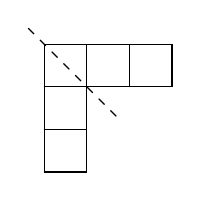
\begin{tikzpicture}
        \node (A) {\ydiagram{3,1,1}};
        \draw[dashed] ($(A.north west) + (135:0.1)$) -- ++ (-45:1.6);
    \end{tikzpicture}
\end{equation}

For each square in a Young tableau we can define a quantity called the
\defineindex{hook number}.
This is the number of squares to the right of or below the square, plus the
square itself.
Most of the time these boxes form a right angled hook shape.
This is shown in \cref{fig:hook length} in detail for \(5 = 3 + 2\).
The hook lengths for all Young tableau's of 5 are given below:
\begin{gather}
    \ytableaushort{54321}\,, \qquad \ytableaushort{5321,1}\,, \qquad
    \ytableaushort{431,21}\,, \qquad \ytableaushort{521,2,1}\,,\\
    \ytableaushort{42,31,1}\,, \qquad \ytableaushort{51,321}\,, \qquad
    \ytableaushort{5,4,3,2,1}\,.
\end{gather}

\begin{figure}
    \tikzsetnextfilename{hook-length}
    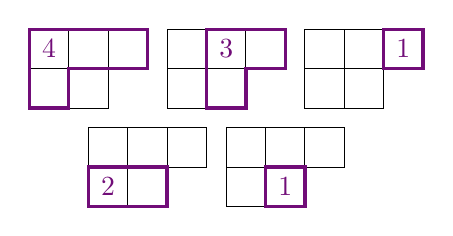
\begin{tikzpicture}[scale=0.5]
        \draw (0, 0) -- (3, 0) -- (3, -1) -- (2, -1) -- (2, -2) -- (0, -2)
        -- cycle;
        \draw (0, -1) -- (2, -1);
        \draw (1, -2) -- (1, 0);
        \draw (2, 0) -- (2, -1);
        \draw[very thick, highlight] (0, 0) -- (3, 0) -- (3, -1) -- (1, -1)
        -- (1, -2) -- (0, -2) -- cycle;
        \node[highlight] at (0.5, -0.5) {4};
        
        \begin{scope}[xshift=3.5cm]
            \draw (0, 0) -- (3, 0) -- (3, -1) -- (2, -1) -- (2, -2) -- (0,
            -2) -- cycle;
            \draw (0, -1) -- (2, -1);
            \draw (1, -2) -- (1, 0);
            \draw (2, 0) -- (2, -1);
            \draw (3, 0) -- (3, -1);
            \draw[very thick, highlight] (1, 0) -- (3, 0) -- (3, -1) -- (2,
            -1) -- (2, -2) -- (1, -2) -- cycle;
            \node[highlight] at (1.5, -0.5) {3};
        \end{scope}
        
        \begin{scope}[xshift=7cm]
            \draw (0, 0) -- (3, 0) -- (3, -1) -- (2, -1) -- (2, -2) -- (0,
            -2) -- cycle;
            \draw (0, -1) -- (2, -1);
            \draw (1, -2) -- (1, 0);
            \draw (2, 0) -- (2, -1);
            \draw (3, 0) -- (3, -1);
            \draw[very thick, highlight] (2, 0) rectangle (3, -1);
            \node[highlight] at (2.5, -0.5) {1};
        \end{scope}
        
        \begin{scope}[yshift=-2.5cm, xshift=1.5cm]
            \draw (0, 0) -- (3, 0) -- (3, -1) -- (2, -1) -- (2, -2) -- (0,
            -2) -- cycle;
            \draw (0, -1) -- (2, -1);
            \draw (1, -2) -- (1, 0);
            \draw (2, 0) -- (2, -1);
            \draw[very thick, highlight] (0, -1) rectangle (2, -2);
            \node[highlight] at (0.5, -1.5) {2};
        \end{scope}
        
        \begin{scope}[yshift=-2.5cm, xshift=5cm]
            \draw (0, 0) -- (3, 0) -- (3, -1) -- (2, -1) -- (2, -2) -- (0,
            -2) -- cycle;
            \draw (0, -1) -- (2, -1);
            \draw (1, -2) -- (1, 0);
            \draw (2, 0) -- (2, -1);
            \draw[very thick, highlight] (1, -1) rectangle (2, -2);
            \node[highlight] at (1.5, -1.5) {1};
        \end{scope}
    \end{tikzpicture}
    \caption[Hook length.]{Calculating the hook lengths for the \(5 = 3 +
        2\) partition. The hook length is the number of squares to the right or below a
        given square, plus the square itself, so in this drawing the hook length of a
        square is the number of squares in the purple hook when that square is at the
        top left of the hook.}
    \label{fig:hook length}
\end{figure}

The reason that we care about the hook length is because there is a rather
remarkable theorem which states that the dimension of a irreducible
representation of \(S_n\) is given by
\begin{equation}
    \dim V_i = \frac{n!}{\prod \text{hook lengths}}
\end{equation}
where the product is of all hook lengths appearing in Young tableau
associated with the representation.
In the case of \(S_5\) this means
\begin{alignat}{5}
    \dim V_1 &= \frac{5!}{5!} &&= 1, \qquad &&\ytableaushort{54321}\,,\\
    \dim V_2 &= \frac{5!}{5\cdot 3!} &&= 4, \qquad &&
    \ytableaushort{5321,1}\,,\\
    \dim V_3 &= \frac{5!}{4!} &&= 5, \qquad && \ytableaushort{431,21}\,,\\
    \dim V_4 &= \frac{5!}{5\cdot 2 \cdot 2} &&= 6\qquad
    &&\ytableaushort{521,2,1}\,,\\
    \dim V_5 &= \frac{5!}{4!} &&= 5 \qquad &&\ytableaushort{42,31,1}\,,\\
    \dim V_6 &= \frac{5!}{5\cdot 3!} &&= 4 \qquad
    &&\ytableaushort{51,321}\,,\\
    \dim V_7 &= \frac{5!}{5!} &&= 1 \qquad && \ytableaushort{5,4,3,2,1}\,.
\end{alignat}
While we won't prove that this works we can check that it doesn't violate
the dimensionality theorem (\cref{thm:dimensionality thm}):
\begin{equation}
    1^2 + 4^2 + 5^2 + 6^2 + 5^2 + 4^2 + 1^1 = 120 = 5! = \abs{S_5}.
\end{equation}

The mirror symmetry between certain pairs of Young tableaus reflects a
symmetry in the character tables.
Namely that if \(\rho\) and \(\rho_{\mathrm{mirror}}\) are irreducible
representations corresponding to Young tableaus which are mirror images then
\begin{equation}
    \chi_{\rho}(g) = \sgn(g)\chi_{\rho_{\mathrm{mirror}}}(g)
\end{equation}
where \(\sgn(g)\) is the sign of the permutation \(g \in S_n\).
Noticing that the \(5 = 3 + 1 + 1\) partition, corresponding to the
\(\rep{6}\) representation, is its own mirror image this must mean that for all
odd \(g \in S_5\) we have \(\chi_{\rep{6}}(g) =
\sgn(g)\chi_{\rep{6}_{\mathrm{mirror}}}(g) = -\chi_{\rep{6}}(g)\), so we have
\(\chi_{\rep{6}}(g) = 0\) for all odd \(g \in S_5\).

\subsection{Direct Product Representations}
So far we have focused on building the irreducible representations.
Given two representations, \(\rho_a \colon G \to \generalLinear(V_1)\) and
\(\rho_b \colon G \to \generalLinear(V_b)\), it is possible to build a new
representation, \(\rho_a \directproduct \rho_b\), called the \defineindex{tensor
    product} of the representations which acts on the tensor product space \(V_a
\directproduct V_b\).
In general this won't be irreducible but can be decomposed.
The fact that \(\rho_a \directproduct \rho_b\) is a representation follows
simply because the direct product of group homomorphisms is another group
homomorphism.
We can decompose \(\rho_a \directproduct \rho_b\) as
\begin{equation}
    \rho_a \directproduct \rho_b = m_{ab}^{1} \rho_{1} \directsum \dotsb
    \directsum m_{ab}^{k} \rho_{\rho_k} = \bigoplus_{c = 1}^{k} m_{ab}^{c} \rho_c',
\end{equation}
with \(m_{ab}^c \in \positiveintegers\).
Direct products of representations are commonly called \define{Kronecker
    products}, or when viewed as a direct sum like this decomposition
\defineindex{Clebsch--Gordan series}.
Since \(\dim(V_a \directproduct V_b) = \dim(V_a) \dim(V_b)\) and \(\dim(V_i
\directproduct V_j) = \dim(V_i) + \dim(V_j)\) it follows that
\begin{equation}
    \dim(V_a)\dim(V_b) = \sum_{c = 1}^{k} m_{ab}^c \dim V_c,
\end{equation}
which is another diophantine equation that can be used to predict the
dimensions of irreducible representations.

\subsubsection{Motivation for Decompositions of Direct Product
    Representations}
There are two motivating arguments for why direct products decompose into
smaller representations.
First, is an argument for finite groups.
The direct product of the largest irreducible representation of a finite
group must decompose since otherwise it is not the largest irreducible
representation (unless one of the representations is one-dimensional, in which
case the direct product isn't really interesting).
This would also cause a conflict with the dimensionality theorem, with the
dimension of the direct product being larger than the order of the group.

There is also a physical argument that the direct product representation
should decompose based on the addition of angular momenta.
This might make more sense after the next chapter on continuous groups.
If a state has angular momentum \(l = 1\) then it transforms as a vector
under \(\specialOrthogonal(3)\).
Consider two three dimensional vectors, \(\vv{v}, \vv{w} \in \reals^3\),
which transforms under an \(l = 1\) irreducible representation of the rotation
group, \(\specialOrthogonal(3)\).
The direct product of these can be written as the vector with components
\begin{equation}
    v_iw_j = A_{ij} + B_{ij}
\end{equation}
where
\begin{equation}
    A_{ij} = v_iw_j - \frac{1}{3}\delta_{ij} \vv{v}\cdot \vv{w}
\end{equation}
is traceless and
\begin{equation}
    B_{ij} = \frac{1}{3}\delta_{ij} \vv{v}\cdot\vv{w}.
\end{equation}
The trace part cannot transform under rotations since it is defined by a
scalar product.
Also the trace is invariant under basis changes, which we can view as a
superset of rotations.
This means \(B_{ij}\) is a scalar (despite having two indices).
This should be clear since \(B_{ij}\) is simply a scalar
(\(\vv{v}\cdot\vv{w}\)) multiple of the identity matrix (\(\delta_{ij}\)).
Scalars transform under an \(l = 0\) irreducible representation of
\(\specialOrthogonal(3)\).

The trace free part has an \(l = 1\) antisymmetric and \(l = 2\) symmetric
irreducible representation.
Motivated by the fact we can get a vector from two vectors via the cross
product, \(\vv{x} = \vv{v} \times \vv{w}\), which is antisymmetric we suppose
that this corresponds to the antisymmetric \(l = 1\) part.
Recalling that addition of angular momentum means two states with angular
momentum \(l_1\) and \(l_2\) can form states with angular momentum \(\abs{l_1 -
    l_2}\), \(\abs{l_1 - l_2} + 1\), and so on up to states with angular momentum
\(l_1 + l_2\) we see that for two \(l = 1\) states we can form states with
angular momentum \(l = 0, 1, 2\).
The reason for this should become clear in the next part when we consider
the Lie group \(\specialOrthogonal(3)\) and the corresponding Lie algebra,
\(\specialOrthogonalLie(3)\).

\subsubsection{Multiplicities}
We can calculate the multiplicities appearing in the decomposition of the
direct product of representations using an inner product:
\begin{align}
    m_{ab}^c &= \innerprod{\chi_{\rho_a \directproduct
            \rho_b}}{\chi_{\rho_c}}\\
    &= \frac{1}{\abs{G}} \sum_{g \in G} \chi_{\rho_{a} \directproduct
        \rho_{b}}(g)^* \chi_{\rho_c}(g)\\
    &= \frac{1}{\abs{G}} \sum_{g \in G} \chi_{\rho_a}(g)^*
    \chi_{\rho_b}(g)^* \chi_{\rho_c}(g).
\end{align}
This leads to the following corollary.

\begin{crl}{}{}
    The Kronecker product of two irreducible representations, \(\rho_a\) and
    \(\rho_b\), contains the trivial representation with multiplicity 1 if and only
    if \(\rho_a = \overline{\rho_b}\).
    \begin{rmk}
        If \(\rho_a\) and \(\rho_b\) are not irreducible then the
        multiplicity can be greater than 1.
    \end{rmk}
    \begin{proof}
        Let \(\rho_a\) and \(\rho_b\) be irreducible representations of some
        finite group \(G\).
        Then
        \begin{align}
            m_{ab}^{\rep{1}} &= \frac{1}{\abs{G}} \sum_{g \in G}
            \chi_{\rho_a}(g)^* \chi_{\rho_b}(g)^*\chi_{\rep{1}}(g)\\
            &= \frac{1}{\abs{G}} \sum_{g \in G} \chi_{\rho_a}(g)^*
            \chi_{\rho_b}(g)^*
        \end{align}
        where we have used the fact that \(\chi_{\rep{1}}(g) = 1\) for all
        \(g \in G\) since \(\rep{1}\) maps all \(g \in G\) to 1.
        Now using the fact that \(\chi_{\rho}(g)^* =
        \chi_{\overline{\rho}}(g)\) we have
        \begin{equation}
            m_{ab}^{\rep{q}} = \frac{1}{\abs{G}}\sum_{g \in G}
            \chi_{\rho_a}(g)\chi_{\overline{b}}(g) =
            \innerprod{\chi_{\rho_a}}{\chi_{\overline{\rho_b}}} = \delta_{a\overline{b}}.
        \end{equation}
        This is 1 if and only if \(\rho_{a} = \overline{\rho_b}\), and zero
        otherwise.
    \end{proof}
\end{crl}

If instead we allowed on or both of the representations above to be
reducible we could simply use the linearity of the inner product to derive a
similar results.

We can use the Kronecker product to understand the mirror representations of
\(S_n\) from \cref{sec:irrep Sn}.
The mirror representation is related to the original representation by a
Kronecker product with the alternating representation.
That is
\begin{equation}
    \rho_{\mathrm{mirror}} = \rho_{\rep{1}'} \directproduct \rho.
\end{equation}

\subsection{Induced Representations}
Induced representations can be thought of as the opposite of branching
rules.
Given two groups, \(G\) and \(H\), with \(H\) a subgroup of \(G\) we can,
given a representation, \(\rho_a \colon H \to \generalLinear(V_a)\), of \(H\)
define a representation of \(G\).

There are two essential steps.
First let \(g_{n_i}\) be representatives of distinct cosets for \(i = 1,
\dotsc, \groupindex{G}{H}\).
Define \(W\) as
\begin{equation}
    W \isomorphic \bigoplus_{i = 1}^{\groupindex{G}{H}} g_{n_i} V_a
\end{equation}
where each \(g_{n_i}V_a\) is an isomorphic copy distinguished by the
\(g_{n_i}\)s from each other.
This means that \(\dim W = \groupindex{G}{H}\dim V_a\).
We can then define some vector \(g_{n_i}\vv{v} \in g_{n_i}V_a\) for \(\vv{v}
\in V_a\).
For different values of \(i\) these will correspond to, by construction,
linearly independent vectors in \(W\).
The second step is to recognise that for arbitrary \(g \in G\) we can write
\begin{equation}
    g g_{n_i} = g_{m_i} h_i
\end{equation}
for some \(h_i \in H\).
This is possible since \(gg_{n_i} \in g_{m_i}H\) for some \(m_i\) since the
left cosets, \(g_{m_i}H\), partition \(G\).
The induced representation is then defined to act on \(\vv{w} \coloneqq
\bigoplus_{i = 1}^{\groupindex{G}{H}} g_{n_i}\vv{v}_{n'_i} \in W\) by
\begin{equation}
    \rho_{\mathrm{induced}}(g) \vv{w} g \bigoplus_{i =
        1}^{\groupindex{G}{H}} g_{n_i}\vv{v}_{n'_i} = \bigoplus_{i =
        1}^{\groupindex{G}{H}} g_{m_i} \rho_a(h_i) \vv{v}_{n'_i}.
\end{equation}
The dimension of the induced representation is the dimension of \(W\).
In general the induced representation is not irreducible.

The regular representation can be seen as the representation induced by the
case where \(H\) is the trivial subgroup and \(\rho_a\) is the trivial
representation.
The vector space is \(V_0 = \reals\) and we identify \(g\vv{v} \in gV_0\) as
\(\ve{g}\) comparing to the notation of the original definition of the regular
representation in \cref{def:regular rep}.

\section{Applications}
\subsection{Distortion of Lattices}
Consider a cubic lattice.
A single cell of this lattice is a cube and so has the symmetry of a cube,
which has symmetry group \(S_4\).
We will consider two distortions of this cube breaking the symmetry from
\(S_4\) to some subgroup.
For simplicity we work with crystallographic coordinates\footnote{see the notes from the Introduction to Condensed Matter Physics.}, where the cube has
corners at \((0, 0, 0)\), \((0, 0, 1)\), \((0, 1, 0)\) and so on.

First, consider a distortion in the \(z\)-direction.
In this case the symmetry breaks to \(D_4\), since we lose the ability to
swap the side faces with the top and so the only symmetries are rotating around
the \(z\) axis and rotating the whole cuboid to swap the top and bottom faces.
This is depicted in \cref{fig:cube z distortion}

\begin{figure}
    \tikzsetnextfilename{cube-distortion-z}
    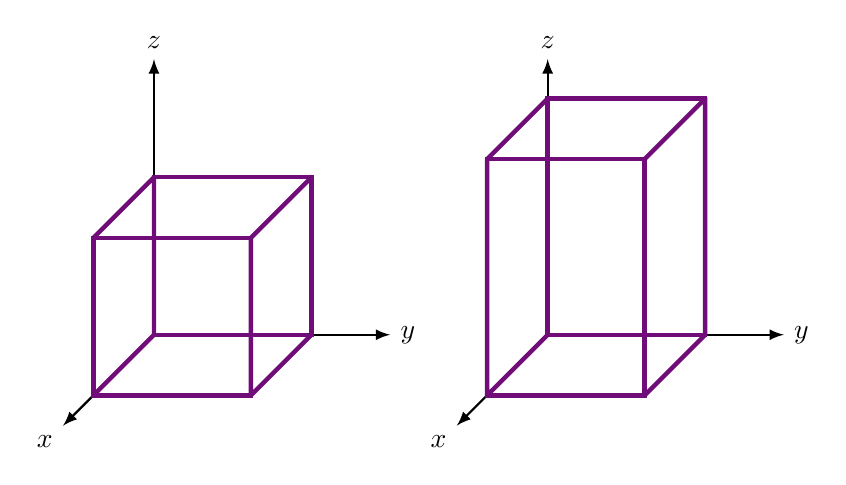
\begin{tikzpicture}
        \draw[thick, ->] (0, 0, 0) -- (3, 0, 0) node[right] {\(y\)};
        \draw[thick, ->] (0, 0, 0) -- (0, 3.5, 0) node[above] {\(z\)};
        \draw[thick, ->] (0, 0, 0) -- (0, 0, 3) node[below left] {\(x\)};
        \draw[ultra thick, highlight] (0, 0, 0) rectangle (2, 2, 0);
        \draw[ultra thick, highlight] (0, 0, 2) rectangle (2, 2, 2);
        \draw[ultra thick, highlight, canvas is yz plane at x=0, rounded
        corners=0.01] (0, 0) rectangle (2, 2);
        \draw[ultra thick, highlight, canvas is yz plane at x=2, rounded
        corners=0.01] (0, 0) rectangle (2, 2);
        \begin{scope}[xshift=5cm]
            \draw[thick, ->] (0, 0, 0) -- (3, 0, 0) node[right] {\(y\)};
            \draw[thick, ->] (0, 0, 0) -- (0, 3.5, 0) node[above] {\(z\)};
            \draw[thick, ->] (0, 0, 0) -- (0, 0, 3) node[below left]
            {\(x\)};
            \draw[ultra thick, highlight] (0, 0, 0) rectangle (2, 3, 0);
            \draw[ultra thick, highlight] (0, 0, 2) rectangle (2, 3, 2);
            \draw[ultra thick, highlight, canvas is yz plane at x=0, rounded
            corners=0.01] (0, 0) rectangle (3, 2);
            \draw[ultra thick, highlight, canvas is yz plane at x=2, rounded
            corners=0.01] (0, 0) rectangle (3, 2);
        \end{scope}
    \end{tikzpicture}
    \caption[A cube distorted along the \(z\)-direction.]{A cube distorted along the \(z\)-direction breaks symmetry
        \(S_4 \to D_4\).}
    \label{fig:cube z distortion}
\end{figure}

Second, consider a distortion in the \((1, 1, 1)\)-direction.
This is depicted in \cref{fig:cube 111 distortion}.
This also breaks the symmetry and the resulting symmetry group is \(D_3\).
This is because we can view the distorted cube along the \((1, 1,
1)\)-direction and end on we see a hexagon with three lines from its centre to
three corners.
This is depicted in \cref{fig:cube corner on}.
This then has the same symmetry as an equilateral triangle, \(D_3\).

\begin{figure}
    \tikzsetnextfilename{cube-distortion-111}
    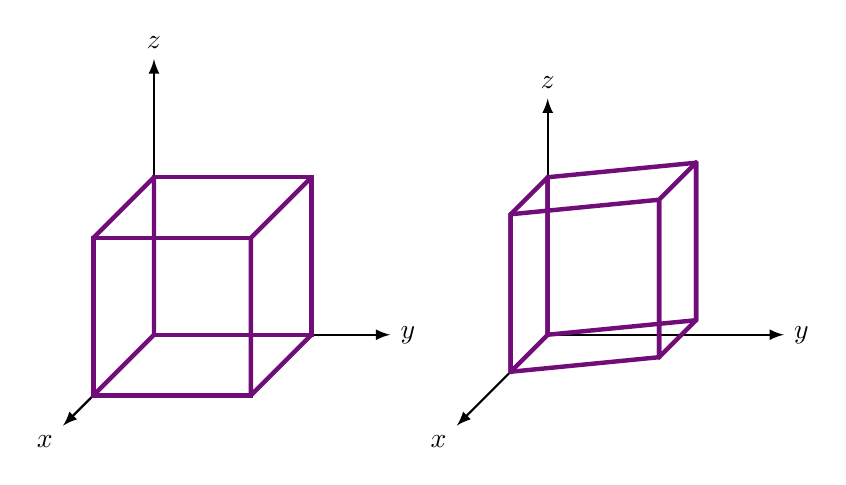
\begin{tikzpicture}
        \draw[thick, ->] (0, 0, 0) -- (3, 0, 0) node[right] {\(y\)};
        \draw[thick, ->] (0, 0, 0) -- (0, 3.5, 0) node[above] {\(z\)};
        \draw[thick, ->] (0, 0, 0) -- (0, 0, 3) node[below left] {\(x\)};
        \draw[ultra thick, highlight] (0, 0, 0) rectangle (2, 2, 0);
        \draw[ultra thick, highlight] (0, 0, 2) rectangle (2, 2, 2);
        \draw[ultra thick, highlight, canvas is yz plane at x=0, rounded
        corners=0.01] (0, 0) rectangle (2, 2);
        \draw[ultra thick, highlight, canvas is yz plane at x=2, rounded
        corners=0.01] (0, 0) rectangle (2, 2);
        \begin{scope}[xshift=5cm]
            \pgfmathsetmacro{\d}{0.3}
            \coordinate (000) at (0, 0, 0);
            \coordinate (001) at (\d, \d, 2);
            \coordinate (010) at (0, 2, 0);
            \coordinate (011) at (\d, \d + 2, 2);
            \coordinate (100) at (2, \d, \d);
            \coordinate (101) at (2 + \d, 2*\d, 2 + \d);
            \coordinate (110) at (2, 2 + \d, \d);
            \coordinate (111) at (2 + \d, 2 + 2*\d, 2 + \d);
            
            \draw[thick, ->] (0, 0, 0) -- (3, 0, 0) node[right] {\(y\)};
            \draw[thick, ->] (0, 0, 0) -- (0, 3, 0) node[above] {\(z\)};
            \draw[thick, ->] (0, 0, 0) -- (0, 0, 3) node[below left]
            {\(x\)};
            \draw[ultra thick, highlight, rounded corners=0.01] (000) --
            (100) -- (110) -- (010) -- cycle;
            \draw[ultra thick, highlight, rounded corners=0.01] (001) --
            (101) -- (111) -- (011) -- cycle;
            \draw[ultra thick, highlight, rounded corners=0.01] (000) --
            (001) -- (011) -- (010) -- cycle;
            \draw[ultra thick, highlight, rounded corners=0.01] (100) --
            (101) -- (111) -- (110) -- cycle;
        \end{scope}
    \end{tikzpicture}
    \caption[A cube distorted along the \((1, 1, 1)\)-direction]{A cube distorted along the \((1, 1, 1)\)-direction breaks
        symmetry \(S_4 \to D_3\).}
    \label{fig:cube 111 distortion}
\end{figure}

\begin{figure}
    \tikzsetnextfilename{cube-corner-on}
    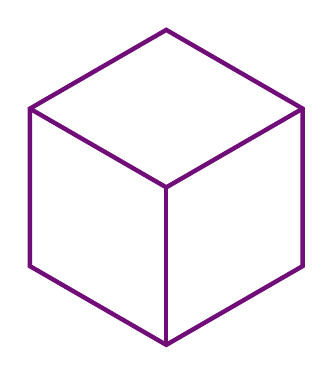
\begin{tikzpicture}
        \foreach \a in {0, 60, ..., 300} {
            \coordinate (\a) at (\a+90:2);
        }
        \draw[ultra thick, highlight] (0) -- (60) -- (120) -- (180) -- (240)
        -- (300) -- cycle;
        \draw[ultra thick, highlight] (60) -- (0, 0);
        \draw[ultra thick, highlight] (180) -- (0, 0);
        \draw[ultra thick, highlight] (300) -- (0, 0);
    \end{tikzpicture}
    \caption[A cube distorted along the \((1, 1, 1)\)-direction viewed point on.]{A cube distorted along the \((1, 1, 1)\)-direction still has
        \(D_3\) symmetry as it can be viewed corner on as depicted here.}
    \label{fig:cube corner on}
\end{figure}

\subsection{Fermi--Bose Statistics}
In quantum mechanics weird things happen when we have identical particles.
In classical mechanics we can (in theory) track the trajectory of each
particle and therefore distinguish even identical particles, based on some
initial arbitrary labelling.
In quantum mechanics we can't do this as there are no trajectories to
follow.

Consider an ensemble of \(N\) non-interacting identical particles.
The state of this system can be written as a tensor product of the states of
the individual particles.
Let \(\hilbert\) be the state space of a single particle and denote by
\(\ket{\varphi_i}\) a single particle state.
Then the state space of the multi-particle system is
\(\hilbert^{\directproduct n}\).
A given state then has the form
\begin{equation}
    \ket{\Phi} = \ket{\varphi_1} \directproduct \ket{\varphi_2}
    \directproduct \dotsb \directproduct \ket{\varphi_N} = \ket{\varphi_1 \directproduct \varphi_2 \directproduct \dotsb \directproduct \varphi_N}
\end{equation}
where the last equality is just a notational convenience.
It should be noted that by the assumption the particles are non-interacting we know they are not entangled and so it is possible to factorise the state into a product of single particle states.
If there were interactions and entanglement this would not be the case and we would have some linear combination of factorised states instead.

The generic state vector can be in any irreducible representation of the symmetric permutation group, \(S_N\), reflecting the fact that we can swap particles.
The question is which representation will it be in?
For large \(N\), say \(N = N_{\mathrm{A}} = \num{6e23}\) the number of irreducible representations is very large.

The two important cases of particles are bosons, particles with integer spin, \(s = 0, 1, 2, \dotsc\), and fermions, particles with half integer spin, \(s = 1/2, 3/2, 5/3, \dotsc\).
For bosons the wave function is in the trivial representation, since exchanging two particles does nothing.
For fermions the wave function is in the alternating representation, since exchanging two particles changes the sign.

As a concrete example consider the case of \(N = 2\).
We then have
\begin{align}
    \ket{\Phi_{\mathrm{bosons}}} &= \frac{\sqrt{2}}{2} (\ket{\varphi_1 \directproduct \varphi_2} + \ket{\varphi_2 \directproduct \varphi_1}),\\
    \ket{\Phi_{\mathrm{fermions}}} &= \frac{\sqrt{2}}{2} (\ket{\varphi_1 \directproduct \varphi_2} - \ket{\varphi_2 \directproduct \varphi_1}).
\end{align}

One of the most important implications of this is that no two fermions can be in the same state, since in this case the wave function would vanish.
This leads to Pauli's exclusion principle.
The fact that this doesn't apply to bosons means that they can all occupy the same energy level, meaning at low temperatures they all fall into the ground state, or other low energy states.
This leads to weird behaviour such as superfluidity and superconductivity.
For fermions this isn't possible so we get a zero point pressure which prevents all of the fermions from being in the ground state.
In a neutron star this zero point pressure balances the gravitational attraction and prevents the star from collapsing into a black hole.

The general connection between spin and statistics, namely that bosons have symmetric wave functions and fermions antisymmetric wave functions, is called the \defineindex{spin statistics theorem}.
Its proof is on quantum field theory and is beyond this course but it relies on a complexification of the Lorentz group.

Perhaps the most surprising thing about all of this is that none of the other representations of \(S_N\) appear.
The statistics of particles acting under these in between representations, known as \defineindex{parastatistics}, can be shown to be equivalent to either the trivial or alternating representation with some extra global symmetry, and therefore they don't bring anything new.
    \part{Continuous Groups}
\chapter{Lie Groups}
\section{Background}
Finite groups were first utilised by mathematicians, particularly Galois, who wanted to classify the solutions to polynomials.
Groups were used to show that, in general, polynomials of degree 5 or greater don't admit an exact solution in terms of elementary functions.
That is, there is no \enquote{quintic formula} equivalent to the quadratic formula.
There are linear, cubic, and quartic versions of the quadratic formula, but the linear formula is trivial and the cubic and quartic formulae contain too many terms to be useful for human computations.
The main focus was on the symmetric groups, since permuting variables in equations played a big part in classifying the solutions, and it was soon noticed that the basic symmetry operations of a group applied to a far more general class of algebraic objects.

Sophus Lie introduced Lie groups, to be defined shortly, for similar reasons, he was attempting to classify solutions to differential equations.
These have continuous solutions and so unsurprisingly Lie groups are continuous.

All simple finite groups have been classified.
Likewise all simple and compact Lie groups have been classified, we will see the classification later.

\section{Basics}
\begin{dfn}{Continuous Group}{}
    A \defineindex{continuous group} is a group, \(G\), with an uncountable number of elements which can be continuously parametrised by some set of parameters, \(\{\alpha\}\).
    We call the number of parameters the \define{dimension}\index{dimension!of a group} of \(G\), \(\dim G\).
\end{dfn}
Notice that it doesn't make sense to discus the order of a continuous group since it is infinite.

\begin{dfn}{Lie Group}{}
    A \define{Lie group}\index{Lie!group} is a continuous group which admits an analytic structure in the parameters \(\{a\}\).
    
    Alternatively, a \define{Lie group} is a manifold equipped with a binary operation satisfying the group axioms.
\end{dfn}
For our purposes a manifold is a space which can be parametrised locally by a fixed number Euclidean coordinates.
The number of coordinates is the dimension of the manifold.
A fuller definition of a manifold is given in \cref{app:manifold}.

All of the groups in the following definition are Lie groups.
Technically, we are only defining a representation of these groups here but this is fine.

\begin{dfn}{Specific Lie Groups}{}
    \begin{itemize}
        \item The \defineindex{general linear group}, \(\generalLinear(n, \field)\), is defined as the group of transformations of an \(n\)-dimensional vector space over \(\field\), which is usually \(\reals\) or \(\complex\).
        It has the representation
        \begin{equation}
            \generalLinear(n, \field) \coloneqq \{M \in \matrices{n}{\field} \mid \det M \ne 0\}.
        \end{equation}
        The requirement of non-zero determinant is so that the matrices are invertible.
        
        \item The \defineindex{special linear group}, \(\specialLinear(n, \field)\), is defined as the group of transformations of an \(n\)-dimensional vector space over \(\field\) which preserve volumes.
        It has the representation
        \begin{equation}
            \specialLinear(n, \field) \coloneqq \{M \in \matrices{n}{\field} \mid \det M \ne 1\} \subgroup \generalLinear(n, \field).
        \end{equation}
        
        \item The \define{orthogonal group}\index{orthogonal!group}, \(\orthogonal(n)\), is defined as the group of transformations of an \(n\)-dimensional vector space over \(\reals\) which preserves lengths.
        It has the representation
        \begin{equation}
            \orthogonal(n) \coloneqq \{O \in \matrices{n}{\reals} \mid O^\trans O = \ident_n\} \subgroup \generalLinear(n, \reals).
        \end{equation}
        
        \item The \defineindex{special orthogonal group}, \(\specialOrthogonal(n)\), is defined as the group of transformations of an \(n\)-dimensional vector space over \(\reals\) which preserves lengths and orientations.
        It has the representation
        \begin{equation}
            \specialOrthogonal(n) \coloneqq \{O \in \matrices{n}{\reals} \mid O^\trans O = \ident_n \text{ and } \det O = 1\}.
        \end{equation}
        It is a subgroup of both \(\orthogonal(n)\) and \(\specialLinear(n, \reals)\).
        
        \item The \define{unitary group}\index{unitary!group}, \(\unitary(n)\), is defined as the group of transformations of an \(n\)-dimensional vector space over \(\complex\) which preserves inner products.
        It has the representation
        \begin{equation}
            \unitary(n) = \{U\in\matrices{n}{\complex} \mid U^\hermit U = \ident_n\} \subgroup \generalLinear(n, \complex).
        \end{equation}
        
        \item The \defineindex{special unitary group}, \(\specialUnitary(n)\), is defined as the group of transformations of an \(n\)-dimensional vector space over \(\complex\) which preserves inner products and orientations.
        It has the representation
        \begin{equation}
            \specialUnitary(n) \coloneqq \{U \in \matrices{n}{\complex} \mid U^\hermit U = \ident_n \text{ and } \det U = 1\}.
        \end{equation}
        It is a subgroup of both \(\unitary(n)\) and \(\specialLinear(n, \complex)\).
        
        \item The \define{symplectic group}\index{symplectic!group}\index{USp(2n)@\(\USp(2n)\), symplectic group of rank \(n\)}\index{SP(n)@\(\Sp(n)\), symplectic group of rank \(n\)}, \(\USp(2n) = \Sp(n)\), is defined as the group of transformations of an \(2n\)-dimensional vector space over \(\field\) which preserves symplectic bilinear forms\footnote{A \define{symplectic bilinear form}\index{symplectic!bilinear form} is a map \(\omega\colon V\times V \to \field\) which is linear in both arguments, alternating, so \(\omega(x, y) = -\omega(y, x)\),  and non-degenerate, so \(\omega(u, v) = 0\) for all \(v \in V\) only if \(u = 0\). We can view \(\reals^{2n}\) as a symplectic space by endowing it with the map \(J\) defined above such that \(\omega(x, y) = x^{\hermit}Jy\).}.
        It has the representation
        \begin{equation}
            \USp(2n) = \Sp(n) \coloneqq \{S \in \matrices{2n}{\field} \mid S^{\hermit} J S = J\}
        \end{equation}
        where
        \begin{equation}
            J \coloneqq
            \begin{pmatrix}
                0 & -\ident_n\\
                -\ident_n & 0
            \end{pmatrix}
            .
        \end{equation}
        Note that \(J^2 = -\ident_{2n}\), so we can think of \(J\) as a generalisation of \(i\) which has \(i^2 = -1\).
    \end{itemize}
\end{dfn}

\begin{exm}{}{}
    The following are group actions of some Lie group on \(\reals^3\).
    \begin{itemize}
        \item \(\reals^3\) with vector addition as the group operation is an \(3\)-dimensional continuous group.
        The parameters can be seen as the components of the vectors.
        
        \item \(\specialOrthogonal(3)\) with matrix multiplication as the group operation is a \(3\)-dimensional continuous group.
        The parameters can be seen as the three Euler angles defining a rotation.
    \end{itemize}
\end{exm}

It should be noted that the dimension of \(\specialOrthogonal(n)\) is not, in general, \(n\).
For example, \(\specialOrthogonal(2)\) has dimension 1, since there is only one parameter defining rotations in the plane, the angle of the rotation.
\(\specialOrthogonal(4)\) has dimension 6, since there are initially \(4^2 = 16\) degrees of freedom for the individual components of the matrix.
It then turns out that orthogonality fixes one component in each row and column, since these must form unit vectors, and the requirement that the determinant is 1 fixes another three degrees of freedom.

\section{Properties of Lie Groups}
There are various properties which manifolds, and hence Lie groups, may or may not posses.
In this section we cover some of these properties.

\subsection{Basic Properties}
\begin{dfn}{Finite or Infinite}{}
    A manifold is finite dimensional if it is parametrised by a finite number of coordinates.
    If this is not the case then the manifold is infinite dimensional.
    A Lie group is \define{finite}\index{finite dimensional Lie group} or \define{infinite dimensional}\index{infinite dimensional Lie group} if it is a finite or infinite dimensional manifold respectively.
\end{dfn}
\begin{exm}{}{}
    The Lie groups \(\unitary(1)\), \(\specialOrthogonal(2)\), \(\specialUnitary(2)\), and \(\specialOrthogonal(3)\) are all finite dimensional.
    
    The Lie group \(\unitary(\hilbert)\) for an infinite dimensional Hilbert space is an infinite dimensional Lie group under the topology induced by the operator norm,
    \begin{equation}
        \norm{A}_{\mathrm{op}} \coloneqq \inf \{c \ge 0 \mid \norm{Av} \le c\norm{v} \text{ for all } v \in \hilbert\}
    \end{equation}
    where \(\norm{-}\) is the norm on \(\hilbert\).
    This norm can be thought of as the smallest number, \(c\), such that \(A\) doesn't scale the \enquote{length} of a vector by more than a factor of \(c\).
    For example, this Lie group might represent all unitary transformations on the state of a particle with a continuous parameter.
\end{exm}

\begin{dfn}{Real or Complex}{}
    A manifold is real if it is parametrised by real numbers with smooth maps, and complex if it is parametrised by complex numbers with holomorphic maps.
    A Lie group is \define{real}\index{real!Lie group} or \define{complex}\index{complex!Lie group} if it is a real or complex manifold, respectively.
\end{dfn}

\begin{dfn}{}{}
    The Lie groups \(\unitary(1)\), \(\specialOrthogonal(2)\), \(\specialUnitary(2)\), and \(\specialOrthogonal(3)\) are real Lie groups, although we will later see that \(\specialUnitary(2)\) is pseudo-real.
\end{dfn}

\subsection{Compactness}    
The following definition assumes the existence of a metric on the manifold.
\begin{dfn}{Compact}{}
    A manifold, \(M\), is compact if it is closed and bounded.
    \define{Bounded}\index{bounded} means that \(d(x, y) < r\) for all \(x, y\) in the manifold and \(r \in \reals\) being some finite number with \(d\) being a metric.
    \define{Closed}\index{closed} means that when viewing \(M\) as a submanifold of some larger manifold \(M\) contains its boundary.
    A Lie group is \define{compact}\index{compact Lie group} if it is compact as a manifold and \define{non-compact}\index{non-compact Lie group} otherwise.
\end{dfn}

As an example consider \(\reals\) with the standard metric \(d(x, y) = \abs{x - y}\).
Then \([0, 1] \coloneqq \{x \in \reals \mid 0 \le x \le 1\}\) is closed and bounded, and hence compact.
The intervals
\begin{align}
    [0, 1) &\coloneqq \{x \in \reals \mid 0 \le x < 1\},\\
    (0, 1] &\coloneqq \{x \in \reals \mid 0 < x \le 1\}, \qand\\
    (0, 1) &\coloneqq \{x \in \reals \mid 0 < x < 1\}
\end{align}
are not closed, but are bounded.
The interval \([0, \infty) \coloneqq \{x \in \reals \mid x > 0\}\) is not bounded since the distance between points can become arbitrarily large.

The circle, \(S^1\), is compact but \(\reals\) isn't.

\begin{exm}{}{}
    The Lie groups \(\unitary(1)\), \(\specialOrthogonal(2)\), \(\specialUnitary(2)\), and \(\specialOrthogonal(3)\) are compact Lie groups.
\end{exm}

For a compact group all of the theorems of \cref{chap:basics of representation theory}, such as Maschke's theorem (\cref{thm:maschke's theorem}), Schur's lemma (\cref{thm:schurs lemma}), and the decomposability theorem (\cref{thm:decomposability}), can be modified to hold for compact continuous groups.
To do so we replace the sum over group elements, \(\sum_{g\in G}\), with the \defineindex{Haar measure}, \(\int \dl{\{\alpha\}}\), we won't go into detail here on this though.
For this reason we will restrict ourselves to compact groups, although here we give a few examples of non-compact groups.

\begin{exm}{Non-Compact Lie Group}{}
    Consider the translation group on \(\reals\).
    That is \(\reals\) acting on \(\reals\) by \(a \action x = x + a\).
    This has a representation, \(\rho \coloneqq \reals \to \generalLinear(V)\), given by the following:
    \begin{equation}
        \rho(a) =
        \begin{pmatrix}
            1 & a\\ 0 & 1
        \end{pmatrix}
        .
    \end{equation}
    However, this doesn't decompose since the subspace defined by the span \(\ve{x} = (1, 0)\) is an invariant subspace but its orthogonal complement, defined by the span of \(\ve{y} = (0, 1)\), is not invariant, since \(\rho(a)\ve{y} = (a, 1) \notin \spn \{\ve{y}\}\).
    Hence we cannot write \(\rho = \rho_1 \directsum \rho_2\) with \(\rho_1 \colon \reals \to \generalLinear(W)\) and \(\rho_2 \colon \reals \to \generalLinear(W^{\bot})\) with \(W \directsum W^{\bot} = V\), despite the fact that \(\rho\) is not irreducible.
    This is a failure of the decomposability theorem (\cref{thm:decomposability}) which holds only for compact groups.
\end{exm}

\begin{exm}{}{}
    The Lorentz group, \(\orthogonal(1, 3)\), is not compact.
    This is because it is parametrised in part by the relative velocity of the frames and this is restricted to the non-compact interval \([0, c)\).
    
    Maschke's theorem (\cref{thm:maschke's theorem}) doesn't hold for the Lorentz group as it has no finite dimensional unitary representations.
    This is why we need to define an invariant of the form \(\bar{\psi}\psi\) for spinors \(\psi\) with \(\bar{\psi} \coloneqq \psi^\hermit \gamma_0\) and \(\gamma_0 \coloneqq \ident_2 \directsum (-\ident_2) = \sigma_3 \directproduct \ident_2\).
    If \(\psi\) instead transformed under a finite dimensional unitary representation, which is guaranteed to exist for a compact group by Maschke's theorem (\cref{thm:maschke's theorem}) then this would not be necessary as \(\psi^\hermit \psi\) would be invariant without the need for \(\gamma_0\).
\end{exm}

\subsection{Connectedness}
\begin{dfn}{}{}
    A manifold is connected if there exists a continuous path between any two points in the manifold.
    A manifold is simply connected if any loop can be contracted continuously to a point.
    A manifold is disconnected if it is not connected.
    A Lie group is \define{disconnected}\index{disconnected Lie group}, \define{connected}\index{connected Lie group}, or \define{simply connected}\defineindex{simply connected Lie group} if it is disconnected, connected, or simply connected as a manifold respectively.
\end{dfn}

Intuitively a space is simply connected if there are no holes.

\begin{figure}
    \tikzsetnextfilename{connected}
    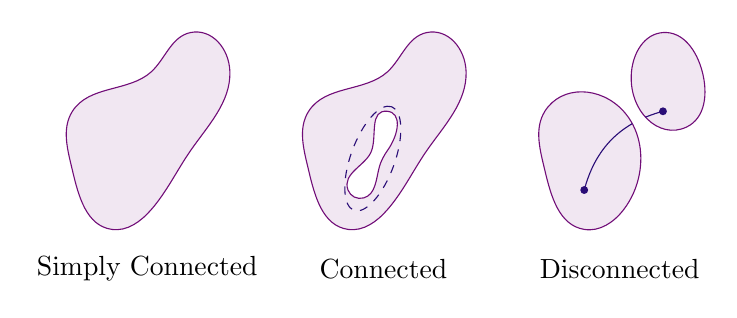
\begin{tikzpicture}
        \node at (0.45, -0.5) {Simply Connected};
        \draw[use Hobby shortcut, closed, highlight, fill=highlight!10] (0, 0) .. (0.5, 0.25) .. (1, 1) .. (1.5, 2) .. (1, 2.5) .. (0.5, 2) .. (-0.5, 1.5) .. (-0.5, 0.75);
        \begin{scope}[xshift=3cm]
            \draw[use Hobby shortcut, closed, highlight, fill=highlight!10] (0, 0) .. (0.5, 0.25) .. (1, 1) .. (1.5, 2) .. (1, 2.5) .. (0.5, 2) .. (-0.5, 1.5) .. (-0.5, 0.75);
            \draw[use Hobby shortcut, closed, highlight, fill=white] (0.2, 0.4) .. (0.4, 0.8) .. (0.5, 1) .. (0.5, 1.5) .. (0.3, 1) .. (0, 0.5);
            \draw[dashed, my blue, rotate around={70:(0.315, 0.9)}] (0.315, 0.9) circle [x radius = 0.7, y radius = 0.28];
            \node at (0.45, -0.5) {Connected};
        \end{scope}
        \begin{scope}[xshift=6cm]
            \draw[use Hobby shortcut, closed, highlight, fill=highlight!10] (1.3, 1.3) .. (1.5, 2) .. (1, 2.5) .. (0.6, 2);
            \draw[use Hobby shortcut, closed, highlight, fill=highlight!10] (0, 0) .. (0.5, 0.25) .. (0.7, 0.7) .. (0.5, 1.5) .. (-0.5, 1.5) .. (-0.5, 0.75);
            \fill[my blue] (0, 0.5) circle [radius = 0.05];
            \fill[my blue] (1, 1.5) circle [radius = 0.05];
            \begin{scope}
                \clip[use Hobby shortcut, closed] (1.3, 1.3) .. (1.5, 2) .. (1, 2.5) .. (0.6, 2);
                \draw[my blue] (0, 0.5) to[bend left] (1, 1.5);
            \end{scope}
            \begin{scope}
                \clip[use Hobby shortcut, closed] (0, 0) .. (0.5, 0.25) .. (0.7, 0.7) .. (0.5, 1.5) .. (-0.5, 1.5) .. (-0.5, 0.75);
                \draw[my blue] (0, 0.5) to[bend left] (1, 1.5);
            \end{scope}
            \node at (0.45, -0.5) {Disconnected};
        \end{scope}
    \end{tikzpicture}
    \caption[Connectedness]{Examples of simply connected, connected, and disconnected spaces. The loop (\tikz[baseline=-2.5pt]{\draw[dashed, my blue] (0, 0) -- ++ (0.5, 0);}) in the connected example cannot be continuously contracted to a point without leaving the space. Similarly the two points (\tikz[baseline=-2.5pt]{\fill[my blue] (0, 0) circle [radius = 0.05];}) in the disconnected example cannot be connected by a continuous path. The path connecting them (\tikz[baseline=-2.5pt]{\draw[my blue] (0, 0) -- ++ (0.5, 0);}) has a jump.}
\end{figure}

\begin{exm}{}{}
    The Lie groups \(\unitary(1)\), \(\specialOrthogonal(2)\), and \(\specialOrthogonal(3)\) are connected.
    The Lie group \(\specialUnitary(2)\) is simply connected.
    The Lie group \(\orthogonal(2)\) is disconnected since there is no continuous path from \(O \in \orthogonal(2)\) with \(\det O = -1\) to \(O' \in \orthogonal\) with \(\det O' = +1\) since \(\det\) is a continuous function and must jump from \(-1\) to \(+1\) along this path somewhere since all orthogonal matrices have \(\abs{\det O} = 1\).
\end{exm}

\subsection{Simplicity}
Recall that a finite group is simple if it has no non-trivial proper normal subgroups, and that a normal subgroup is one which is invariant under conjugation.
That is, \(N \normalsubgroup G\) if \(gng^{-1} \in N\) for all \(n \in n\) and \(g \in G\).
We define simple Lie groups in a similar way but we explicitly disallow a few cases.

\begin{dfn}{Simple Lie Group}{}
    A Lie group is \define{simple}\index{simple group} if it is connected, non-Abelian, and has no non-trivial connected normal subgroups.
    
    A \defineindex{semi-simple Lie group} is a Lie group which can be written as a direct product of simple Lie groups.
    
    A \defineindex{composite Lie group} is a Lie group which can be written as a semi-direct product of simple Lie groups.
\end{dfn}

The reason we exclude more cases than for the definition for any group is motivated by the fact that it is not possible to define a quotient group from a simple group, apart from the trivial group and the simple group itself.
We want this to hold replacing all groups with Lie groups.
Importantly this means that we want a simple Lie group to be one where it is not possible to define a non-trivial quotient \emph{Lie} group.
If we expand upon what this requires we get the definition above.

We will only concern ourselves with simple Lie groups in this course.

\begin{exm}{}{}
    The Lie groups \(\specialLinear(n)\), \(\specialUnitary(n)\), and \(\USp(2n) = \Sp(n)\) are simple.
\end{exm}

\subsubsection{Classification of Simple Compact Lie Groups}
All simple compact Lie groups have been classified.
It turns out there are four families of simple compact Lie groups, \(A_n\), \(B_n\), \(C_n\), and \(D_n\), and five exceptional groups, \(E_6\), \(E_7\), \(E_8\), \(F_4\), and \(G_2\) which don't fall into any of these categories.
We won't define the exceptional groups here, we just note that they exist.
The families consist of familiar groups, \(A_n = \specialUnitary(n + 1)\), \(B_n = \specialOrthogonal(2n + 1)\), \(C_n = \USp(2n)\), and \(D_n = \specialOrthogonal(2n)\).
These are sorted by their rank, which is given by the subscript.
Rank is a concept related to the Lie algebras of these groups, which we shall meet later.

\begin{table}
    \begin{tabular}{lcc}\toprule
        Group & Dimension & Rank \\ \midrule
        \(A_n\) & \((n + 1)^2 - 1\) & \(n\)\\
        \(B_n\) & \(n(2n + 1)\) & \(n\)\\
        \(C_n\) & \(n(2n + 1)\) & \(n\)\\
        \(D_n\) & \(n(2n - 1)\) & \(n\)\\ \midrule
        \(E_6\) & 78 & 6\\
        \(E_7\) & 133 & 7\\
        \(E_8\) & 248 & 8\\
        \(F_4\) & 52 & 4\\
        \(G_2\) & 14 & 2\\ \bottomrule
    \end{tabular}
    \caption{Classification of simple compact Lie groups}
\end{table}

\tikzset{dynkin node/.style = {fill = white}}
\tikzset{->-/.style = {decoration={markings, mark=at position #1 with {\arrow{>}}}, postaction={decorate}}}
\tikzset{-<-/.style = {decoration={markings, mark=at position #1 with {\arrow{<}}}, postaction={decorate}}}
The Lie groups can be depicted by \define{Dynkin diagrams}\index{Dynkin diagram}, which are graphs with as many nodes as the rank\footnote{to be defined in \cref{sec:lie algebra generalities}} of the group.
For example, \(A_1\) corresponds to
\tikzsetnextfilename{dynkin-A1}
\tikz[baseline=-2.5pt]{ \draw[dynkin node] (0, 0) circle [radius = 0.075]; }
, \(A_2\) corresponds to
\tikzsetnextfilename{dynkin-A2}
\tikz[baseline=-2.5pt]{ \draw (0, 0) -- (1, 0); \draw[dynkin node] (0, 0) circle [radius = 0.075]; \draw[dynkin node] (1, 0) circle [radius =0.075]; }
, and \(A_3\) corresponds to
\tikzsetnextfilename{dynkin-A3}
\tikz[baseline=-2.5pt]{ \draw (0, 0) -- (2, 0); \draw[dynkin node] (0, 0) circle [radius = 0.075]; \draw[dynkin node] (1, 0) circle [radius =0.075]; \draw[dynkin node] (2, 0) circle [radius =0.075]; }
.
In general \(A_n\) corresponds to
\tikzsetnextfilename{dynkin-An}
\tikz[baseline=-2.5pt]{ \draw (0, 0) -- (1.3, 0); \draw (1.7, 0) -- (3, 0); \draw[dotted] (1.3, 0) -- (1.7, 0); \draw[dynkin node] (0, 0) circle [radius = 0.075]; \draw[dynkin node] (1, 0) circle [radius =0.075]; \draw[dynkin node] (2, 0) circle [radius =0.075]; \draw[dynkin node] (3, 0) circle [radius =0.075]; }
with \(n\) nodes.

The Dynkin  diagram for \(B_n\) is similar but the final connection is doubled and directed, so \(B_2\) corresponds to
\tikzsetnextfilename{dynkin-B2}
\tikz[baseline=-2.5pt]{ \draw[double, ->-=0.65, >=To] (0, 0) -- (1, 0); \draw[dynkin node] (0, 0) circle [radius = 0.075]; \draw[dynkin node] (1, 0) circle [radius =0.075]; }
, and \(B_3\) corresponds to
\tikzsetnextfilename{dynkin-B3}
\tikz[baseline=-2.5pt]{ \draw (-1, 0) -- (0, 0); \draw[double, ->-=0.65, >=To] (0, 0) -- (1, 0); \draw[dynkin node] (-1, 0) circle [radius = 0.075]; \draw[dynkin node] (0, 0) circle [radius = 0.075]; \draw[dynkin node] (1, 0) circle [radius =0.075]; }
.
In general \(B_n\) corresponds to
\tikzsetnextfilename{dynkin-Bn}
\tikz[baseline=-2.5pt]{ \draw (-2, 0) -- (-0.7, 0); \draw (-0.3, 0) -- (0, 0); \draw[dotted] (-0.7, 0) -- (-0.3, 0); \draw[double, ->-=0.65, >=To] (0, 0) -- (1, 0); \draw[dynkin node] (-2, 0) circle [radius = 0.075]; \draw[dynkin node] (-1, 0) circle [radius = 0.075]; \draw[dynkin node] (0, 0) circle [radius = 0.075]; \draw[dynkin node] (1, 0) circle [radius =0.075]; }
with \(n\) nodes.

The Dynkin diagrams for \(C_n\) are almost identical to those of \(B_n\) but with the direction reversed, so \(C_2\) corresponds to
\tikzsetnextfilename{dynkin-C2}
\tikz[baseline=-2.5pt]{ \draw[double, -<-=0.65, >=To] (0, 0) -- (1, 0); \draw[dynkin node] (0, 0) circle [radius = 0.075]; \draw[dynkin node] (1, 0) circle [radius =0.075]; }
, and \(C_3\) corresponds to
\tikzsetnextfilename{dynkin-C3}
\tikz[baseline=-2.5pt]{ \draw (-1, 0) -- (0, 0); \draw[double, -<-=0.65, >=To] (0, 0) -- (1, 0); \draw[dynkin node] (-1, 0) circle [radius = 0.075]; \draw[dynkin node] (0, 0) circle [radius = 0.075]; \draw[dynkin node] (1, 0) circle [radius =0.075]; }
.
In general \(C_n\) corresponds to
\tikzsetnextfilename{dynkin-Cn}
\tikz[baseline=-2.5pt]{ \draw (-2, 0) -- (-0.7, 0); \draw (-0.3, 0) -- (0, 0); \draw[dotted] (-0.7, 0) -- (-0.3, 0); \draw[double, -<-=0.65, >=To] (0, 0) -- (1, 0); \draw[dynkin node] (-2, 0) circle [radius = 0.075]; \draw[dynkin node] (-1, 0) circle [radius = 0.075]; \draw[dynkin node] (0, 0) circle [radius = 0.075]; \draw[dynkin node] (1, 0) circle [radius =0.075]; }
with \(n\) nodes.

The Dynkin diagrams for \(D_n\) branch at the end into two.
So \(D_4\) corresponds to 
\begin{equation}
    \tikzsetnextfilename{dynkin-D4}
    \tikz[baseline=(current bounding box.east)]{ \draw (0, 0) -- (1, 0); \draw (1, 0) -- ++ (30:1); \draw (1, 0) -- ++ (-30:1); \draw[dynkin node] (0, 0) circle [radius = 0.075]; \draw[dynkin node] (1, 0) circle [radius = 0.075]; \draw[dynkin node] ($(1, 0) + (30:1)$) circle [radius = 0.075]; \draw[dynkin node] ($(1, 0) + (-30:1)$) circle [radius = 0.075]; }
\end{equation}
and \(D_5\) corresponds to
\begin{equation}
    \tikzsetnextfilename{dynkin-D5}
    \tikz[baseline=(current bounding box.east)]{ \draw (-1, 0) -- (1, 0); \draw (1, 0) -- ++ (30:1); \draw (1, 0) -- ++ (-30:1); \draw[dynkin node] (-1, 0) circle [radius = 0.075]; \draw[dynkin node] (0, 0) circle [radius = 0.075]; \draw[dynkin node] (1, 0) circle [radius = 0.075]; \draw[dynkin node] ($(1, 0) + (30:1)$) circle [radius = 0.075]; \draw[dynkin node] ($(1, 0) + (-30:1)$) circle [radius = 0.075]; }
\end{equation}
In general, \(D_n\) corresponds to
\begin{equation}
    \tikzsetnextfilename{dynkin-Dn}
    \tikz[baseline=-2.5pt]{ \draw (-1, 0) -- (0.3, 0); \draw (0.7, 0) -- (1, 0); \draw[dotted] (0.3, 0) -- (0.7, 0); \draw (1, 0) -- ++ (30:1); \draw (1, 0) -- ++ (-30:1); \draw[dynkin node] (-1, 0) circle [radius = 0.075]; \draw[dynkin node] (0, 0) circle [radius = 0.075]; \draw[dynkin node] (1, 0) circle [radius = 0.075]; \draw[dynkin node] ($(1, 0) + (30:1)$) circle [radius = 0.075]; \draw[dynkin node] ($(1, 0) + (-30:1)$) circle [radius = 0.075]; }
\end{equation}

The exceptional groups also have Dynkin diagrams.
For \(E_n\) (\(n = 6, 7, 8\)) the Dynkin diagram consists of a chain of \(n - 1\) nodes with an extra node branching off three from the end, so \(E_6\) corresponds to
\begin{equation}
    \tikzsetnextfilename{dynkin-E6}
    \begin{tikzpicture}[baseline=(current bounding box.east)]
        \draw (0, 0) -- (4, 0);
        \draw (2, 0) -- (2, 1);
        \foreach \x in {0, ..., 4} {
            \draw[dynkin node] (\x, 0) circle [radius = 0.075];
        }
        \draw[dynkin node] (2, 1) circle [radius = 0.075];
    \end{tikzpicture}
\end{equation}
\(E_7\) corresponds to
\begin{equation}
    \tikzsetnextfilename{dynkin-E7}
    \begin{tikzpicture}[baseline=(current bounding box.east)]
        \draw (0, 0) -- (5, 0);
        \draw (3, 0) -- (3, 1);
        \foreach \x in {0, ..., 5} {
            \draw[dynkin node] (\x, 0) circle [radius = 0.075];
        }
        \draw[dynkin node] (3, 1) circle [radius = 0.075];
    \end{tikzpicture}
\end{equation}
and \(E_8\) to
\begin{equation}
    \tikzsetnextfilename{dynkin-E8}
    \begin{tikzpicture}[baseline=(current bounding box.east)]
        \draw (0, 0) -- (6, 0);
        \draw (4, 0) -- (4, 1);
        \foreach \x in {0, ..., 6} {
            \draw[dynkin node] (\x, 0) circle [radius = 0.075];
        }
        \draw[dynkin node] (4, 1) circle [radius = 0.075];
    \end{tikzpicture}
\end{equation}

The Dynkin diagram for \(F_4\) is
\tikzsetnextfilename{dynkin-F4}
\tikz[baseline=-2.5pt]{ \draw (0, 0) -- (1, 0); \draw[double, ->-=0.65, >=To] (1, 0) -- (2, 0); \draw (2, 0) -- (3, 0); \draw[dynkin node] (0, 0) circle [radius = 0.075]; \draw[dynkin node] (1, 0) circle [radius = 0.075]; \draw[dynkin node] (2, 0) circle [radius = 0.075]; \draw[dynkin node] (3, 0) circle [radius = 0.075];}
.

The Dynkin diagram for \(G_2\) is
\tikzsetnextfilename{dynkin-G2}
\tikz[baseline=-2.5pt]{ \draw[->-=0.65, >={To[width=0.3cm, length=0.14cm]}] (0, 0) -- (1, 0); \draw[yshift=0.035cm] (0, 0) -- (1, 0); \draw[yshift=-0.035cm] (0, 0) -- (1, 0); \draw[dynkin node] (0, 0) circle [radius = 0.075]; \draw[dynkin node] (1, 0) circle [radius = 0.075]; }
.

Notice that for some low-rank cases the Dynkin diagrams are degenerate, for example \(A_1\) and \(B_1\) both correspond to
\tikzsetnextfilename{dynkin-B1}
\tikz[baseline=-2.5pt]{ \draw[dynkin node] (0, 0) circle [radius = 0.075]; }
which reflects the fact that \(A_1 \cong B_1\), which is to say \(SU(2) \cong SO(3)\), a fact that will be important later.
It also explains why the \(E_n\) exceptional groups start at \(E_6\), since the Dynkin diagram for \(E_5\) is the same as for \(D_5\), and the Dynkin diagram for \(E_4\) is the same as for \(A_4\).

\chapter{Lie Algebras}
A lot of the uses of Lie groups make use of the underlying analytic structure to expand the group elements in the parameters, \(\{\alpha\}\), and then keep only the first order terms, linearising the group.
Mathematically this is what we do if we move to the tangent space of the manifold and we call the resulting linear space the \define{Lie algebra}\index{Lie!algebra} associated with the Lie group.
We will start with a simple example which we will then generalise.

\section{The Abelian Group \texorpdfstring{\(\unitary(1) \isomorphic \specialOrthogonal(2)\)}{U(1) isomorphic to SO(2)}}
We can define the unitary group \(\unitary(1)\) as
\begin{equation}
    \unitary(1) \coloneqq \{ U \in \matrices{1}{\complex} \mid U^\hermit U = \ident \}.
\end{equation}
This is obviously the same as the circle group
\begin{equation}
    \mathbb{T} \coloneqq \{ z \in \complex \mid \abs{z} = 1 \}
\end{equation}
under the obvious isomorphism associating \((z) \in \unitary(1)\) with \(z \in \mathbb{T}\).
We therefore don't distinguish between \(\unitary(1)\) and \(\mathbb{T}\) and will say things like \(z \in \unitary(1)\), when it may be more proper to say \((z) \in \unitary(1)\).
As the name suggests \(\mathbb{T}\) is a Lie group with the circle, \(S^1\), as its underlying manifold.
This is a one-dimensional real manifold parametrised by \(\alpha \in [0, 2\pi)\).

We can define the two dimensional rotation group, \(\specialOrthogonal(2)\), as
\begin{equation}
    \specialOrthogonal(2) \coloneqq \{ R \in \matrices{2}{\reals} \mid R^\trans R = \ident \text{ and } \det R = 1 \}.
\end{equation}
This acts on the plane, \(\reals^2\), through rotations, which are given by normal matrix multiplication, \(R \action \vv{x} = R\vv{x}\).
This is a one dimensional real manifold parametrised by the rotation angle, \(\alpha \in [0, 2\pi)\).

The unitary group \(\unitary(1)\) has an infinite family of representations labelled by \(n \in \integers\) given by
\begin{equation}
    \rho_n^{\unitary(1)}(\alpha) = \e^{in\alpha}.
\end{equation}
Here we are implicitly associating complex numbers with \(1\times 1\) complex matrices.
The two-dimensional rotation group, \(\specialOrthogonal(2)\), has an infinite family of representations labelled by \(n \in \integers\) given by
\begin{equation}
    \rho_n^{\specialOrthogonal(2)}(\alpha) =
    \begin{pmatrix}
        \cos(n\alpha) & \sin(n\alpha)\\
        -\sin(n\alpha) & \cos(n\alpha)
    \end{pmatrix}
    .
\end{equation}
It should be clear that \(\unitary(1)\) and \(\specialOrthogonal(2)\) are isomorphic.
One isomorphism between them being \(\e^{i\alpha} \mapsto \rho_{1}^{\specialOrthogonal(2)}(\alpha)\).
Since this is the case we will move between them as needed choosing which ever is most appropriate for the task at hand.

The Kronecker product of representation is particularly simple for this case with
\begin{equation}
    \rho_{n} \directproduct \rho_{m} = \rho_{n + m}.
\end{equation}

In order to linearise \(\specialOrthogonal(2)\) we make use of the fact that elements of \(\unitary(1)\) can be expressed as \(\e^{i\alpha}\) and we suggest that \(O \in \specialOrthogonal(2)\) can be expressed as\footnote{the factor of \(i\) appearing in the exponent is a matter of convention, typically physicists include it and mathematicians absorb it in the definition of \(T\), which results in slightly different requirements on \(T\), in particular \(T\) will be anti-Hermitian (or skew-Hermitian), so \(T^\hermit = -T\)}
\begin{equation}
    O = \exp[i\alpha T]
\end{equation}
for some \(T \in \matrices{2}{\reals}\).
As usual the exponential of a matrix is to be understood either through its power series,
\begin{equation}
    \exp(A) = \sum_{n = 0}^{\infty} \frac{A^n}{n!},
\end{equation}
or a limit,
\begin{equation}
    \exp(A) = \lim_{n \to \infty} \left( 1 + \frac{A}{n} \right)^{n}.
\end{equation}

\begin{lma}{}{}
    Let \(A \in \matrices{m}{\complex}\) be diagonalisable.
    Then \(\det(\exp(A)) = \exp(\tr(A))\).
    
    \begin{rmk}
        This theorem also holds for non-diagonalisable matrices.
        One way to show this involves the Jordan normal form.
        Another way is to note that diagonalisable matrices are dense in \(\matrices{n}{\complex}\) and so every \(A \in \matrices{n}{\complex}\) can be written as an infinite series of diagonalisable matrices.
        We can then apply this proof to the terms of the series and the fact that \(\tr\) and \(\det\) are continuous guarantees the result holds as if we were to apply the theorem to the original matrix.
    \end{rmk}
    
    \begin{proof}
        Let \(A \in \matrices{m}{\complex}\) be diagonalisable.
        We work in the basis in which \(A\) is diagonal since both \(\det\) and \(\tr\) are basis independent.
        In this basis the diagonal of \(A\) consists of its eigenvalues, \(\lambda_i\).
        We then have
        \begin{equation}
            \det A = \prod_{i = 1}^{m} \lambda_i,
        \end{equation}
        and
        \begin{equation}
            \tr A = \sum_{i = 1}^{m} \lambda_i.
        \end{equation}
        Further in this basis \(\exp(A)\) is diagonal and its diagonal components are \(\exp(\lambda_i)\).
        This follows since the \(n\)th power of a diagonal matrix just raises the elements on the diagonal to the \(n\)th power, that is
        \begin{equation}
            \begin{pmatrix}
                \lambda_1 &&\\
                &\ddots &\\
                && \lambda_m
            \end{pmatrix}
            ^n = 
            \begin{pmatrix}
                \lambda_1^n &&\\
                &\ddots &\\
                && \lambda_m^n
            \end{pmatrix}
            .
        \end{equation}
        It follows that
        \begingroup
        \allowdisplaybreaks
        \begin{align}
            \exp(A) &= \sum_{n = 0}^{\infty} \frac{A^n}{n!}\\
            &= \sum_{n = 0}^{\infty} \frac{1}{n!} 
            \begin{pmatrix}
                \lambda_1 && \\
                & \ddots & \\
                && \lambda_m
            \end{pmatrix}
            ^n\\
            &= \sum_{n = 0}^{\infty} \frac{1}{n!}
            \begin{pmatrix}
                \lambda_1^n && \\
                & \ddots & \\
                && \lambda_m^n
            \end{pmatrix}
            \\
            &= 
            \begin{pmatrix}
                \sum_{n = 0}^{\infty} \frac{\lambda_1^n}{n!} && \\
                & \ddots & \\
                && \sum_{n = 0}^{\infty} \frac{\lambda_m^n}{n!}
            \end{pmatrix}
            \\
            &= 
            \begin{pmatrix}
                \exp(\lambda_1) && \\
                & \ddots & \\
                && \exp(\lambda_m)
            \end{pmatrix}
        \end{align}
        \endgroup
        Hence
        \begin{align}
            \exp(\tr(A)) &= \exp\left( \sum_{i} \lambda_i \right)\\
            &= \prod_{i} \exp(\lambda_i)\\
            &= \det(\exp(A)).
        \end{align}
    \end{proof}
\end{lma}

An alternative statement of this theorem is that the following diagram commutes.
That is, the result is the same no matter what path you follow.
\begin{equation}
    \tikzexternaldisable
    \begin{tikzcd}
        \lie{g} \arrow[r, "\exp"] \arrow[d, "\tr"'] & G \arrow[d, "\det"] \\
        \complex \arrow[r, "\exp"'] & \complex.
    \end{tikzcd}
    \tikzexternalenable
\end{equation}
Here \(G\) is a Lie group, and \(\lie{g}\) is its Lie algebra (to be defined).
Note that there are two subtly different functions called \(\exp\) here, one is a function \(\complex \to \complex\), whereas the other is a function \(\lie{g} \to G\), or more generally from the tangent space, \(T_eM\), to the manifold, \(M\).
Both can be defined through equivalent power series and agree when \(G\) is one-dimensional.

The definition of \(O \in \specialOrthogonal(2)\) is that \(O^\trans O = \ident\), which can be expressed as
\begin{align}
    \ident &= O^\trans O\\
    &= \exp(i\alpha T)^{\trans} \exp(i\alpha T)\\
    &= \exp(i\alpha T^{\trans}) \exp(i\alpha T)\\
    &= (\ident + i\alpha T^{\trans} + \order(\alpha^2))(\ident + i\alpha T + \order(\alpha^2))\\
    &= \ident + i\alpha(T^\trans + T) + \order(\alpha^2).
\end{align}
Therefore if we take \(\alpha\) to be small we have that \(T^{\trans} = -T\), which is to say that \(T\) must be antisymmetric.
This in fact generalises to \(\specialOrthogonal(n)\), we can write any element as \(\exp(i\alpha T)\) where \(T \in \matrices{n}{\reals}\) is antisymmetric.

One particular solution is
\begin{equation}
    T = i
    \begin{pmatrix}
        0 & 1\\
        -1 & 0
    \end{pmatrix}
    ,
\end{equation}
which leads to the previous representation since \(T^2 = \ident\) and so
\begin{equation}
    \exp(i\alpha T) = \ident \cos(\alpha) + iT\sin(\alpha) = \rho_1^{\specialOrthogonal(2)}(\alpha).
\end{equation}
This follows by expanding the exponential and collecting even and odd terms.

We define the Lie algebra of \(\specialOrthogonal(2)\) to be all (real) scalar multiples of \(T\), \(\specialOrthogonalLie(2) \coloneqq \{\lambda T \mid \lambda \in \reals\}\).
This is fairly boring since there is only one dimension, but it is useful to demonstrate the tangent space notion of the Lie algebra.

As previously mentioned the underlying manifold for \(\unitary(1)\), and hence \(\specialOrthogonal(2)\), is the circle, \(S^1 = \{(x, y) \in \reals^2 \mid x^2 + y^2 = 1\}\), strictly this is an embedding of \(S^1\) in two-dimensions, on its own \(S^1\) is a one-dimensional manifold.
We can cover \(S^1\) with two charts, two are needed to avoid a discontinuity at the join, we simply use whichever hasn't got the join at that point.
For example, one chart could be \(f_1(\vartheta) = (\cos\vartheta, \sin\vartheta)\) and another \(f_2(\vartheta) = (\cos(\vartheta - \pi/2), \sin(\vartheta - \pi/2))\), which is just \(f_1\) rotated around by \(\pi/2\).
Both of these maps have the codomain \([0, 2\pi)\).

Now consider the point \((x, y)\) on \(S^1\).
We have \(T(x, y) = (-y, x)\).
For example, if \(T(-1, 0) = (0, -1)\).
This vector will be tangent to \(S^1\) as embedded in \(\reals^2\).

\begin{figure}
    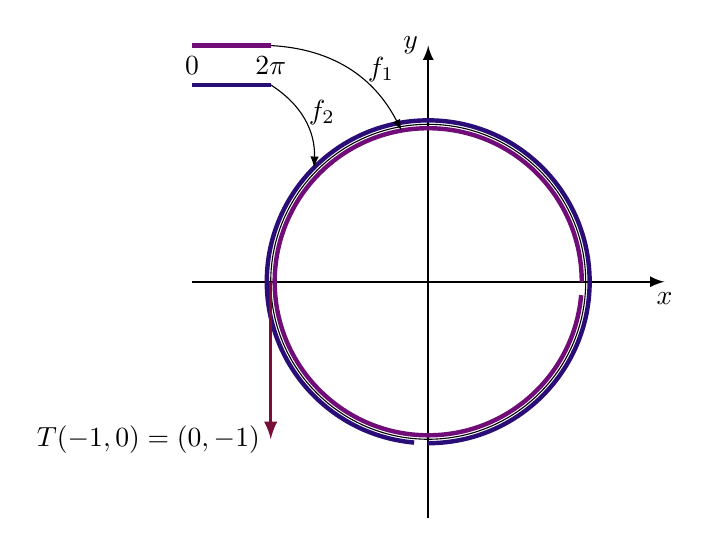
\begin{tikzpicture}
        \draw[thick, ->] (-3, 0) -- (3, 0) node[below] {\(x\)};
        \draw[thick, ->] (0, -3) -- (0, 3) node[left] {\(y\)};
        \draw (0, 0) circle [radius = 2];
        \draw[ultra thick, highlight] (1.95, 0) arc (0:355:1.95);
        \draw[ultra thick, my blue, rotate=-90] (2.05, 0) arc (0:355:2.05);
        \draw[ultra thick, highlight] (-3, 3) -- ++ (1, 0) coordinate (A);
        \draw[->] (A) to[bend left] (100:1.95);
        \node at (-0.6, 2.7) {\(f_1\)};
        \draw[ultra thick, my blue] (-3, 2.5) -- ++ (1, 0) coordinate (B);
        \draw[->] (B) to[bend left] (135:2.05);
        \node at (-1.35, 2.15) {\(f_2\)};
        \draw[my red, very thick, ->] (-2, 0) -- ++ (0, -2) node[left, black] {\(T(-1, 0) = (0, -1)\)};
        \node at (-3, 2.75) {0};
        \node at (-2, 2.75) {\(2\pi\)};
    \end{tikzpicture}
    \caption[The manifold \(S^1\)]{The manifold \(S^1\) covered by two charts, \(f_1\) and \(f_2\). \(T(x, y)\) gives a tangent vector as demonstrated by the case of \((x, y) = (-1, 0)\). The slight gaps in the two charts represent the discontinuity in \(\alpha\) going from 0 to \(2\pi\). Either chart is valid away from these discontinuities and at a discontinuity simply use the continuous chart.}
\end{figure}

The manifold \(\specialOrthogonal(2)\) is connected, since \(S^1\) is clearly connected.
On the other hand the manifold \(\orthogonal(2)\) is \emph{not} connected.
It is formed from two disconnected pieces, one, which has \(\det O = 1\), is essentially a copy of \(\specialOrthogonal(2)\), and one where \(\det O = -1\).
These two pieces are disconnected since \(\det\) is a continuous function of the parameters yet makes a sudden jump from \(-1\) to \(+1\), which can only happen if there is a corresponding sudden jump in the parameters, meaning that \(\orthogonal(2)\) is not connected.

Consider the parity operator
\begin{equation}
    P = 
    \begin{pmatrix}
        1 & 0\\
        0 & -1
    \end{pmatrix}
    .
\end{equation}
This is an element of \(\orthogonal(2)\), but not \(\specialOrthogonal(2)\).
Since \(P^2 = \ident\) we can view \(P\) as generating \(\integers_2 = \presentation{P}{P^2 = \ident}\) and we can then identify
\begin{equation}
    \specialOrthogonal(2) \isomorphic \orthogonal(2) / \integers_2.
\end{equation}
In fact, this generalises to
\begin{equation}
    \specialOrthogonal(n) \isomorphic \orthogonal(n) / \integers_2.
\end{equation}
Further we have
\begin{equation}
    \specialUnitary(n) \isomorphic \unitary(n) / \unitary(1)
\end{equation}
since we can think of \(\unitary(1)\) as the complex version of \(\integers_2\).

For \(\specialOrthogonal(2)\) the Haar measure is
\begin{equation}
    \int_0^{2\pi} \frac{\dl{\alpha}}{2\pi}
\end{equation}
and so we can define an inner product on the character space as
\begin{align}
    \innerprod{\chi_{\rho_n}}{\chi_{\rho_m}}_{\unitary(1)} &= \frac{1}{2\pi}\int_{0}^{2\pi} \chi_{\rho_n}(\alpha)^* \chi_{\rho_m}(\alpha) \dd{\alpha}\\
    &= \frac{1}{2\pi} \int_{0}^{2\pi} (\e^{in\alpha})^*\e^{im\alpha} \dd{\alpha}\\
    &= \frac{1}{2\pi} \int_{0}^{2\pi} \e^{i(n - m)\alpha} \dd{\alpha}\\
    &= \delta_{nm}.
\end{align}
We see that the characters are orthonormal with respect to this inner product.
The characters turn out to be less important for Lie groups than finite groups and we won't consider them much more.

\section{Lie Algebra Generalities}\label{sec:lie algebra generalities}
\begin{thm}{Exponential Map}{}
    Every one-parameter subgroup of \(\generalLinear(n, \complex)\) is given by a matrix exponential, \(\rho_T(t) = \exp(tT)\) where \(T \in \matrices{n}{\complex}\) and \(T\) is not the zero matrix.
    \begin{rmk}
        We call \(T\) the \defineindex{generator} of the one-parameter subgroup.
    \end{rmk}
    \begin{proof}
        Consider the single parameter homomorphism \(\rho_T \colon \reals \to \generalLinear(n, \complex)\) defined by
        \begin{equation}
            \diff*{\rho_T(t)}{t}[t = 0] = T
        \end{equation}
        with the boundary condition \(\rho_T(0) = \ident\).
        Since \(\rho_T\) is a group homomorphism we require
        \begin{equation}
            \rho_T(s + t) = \rho_T(s)\rho_T(t).
        \end{equation}
        Differentiating this with respect to \(s\) and evaluating at \(s = 0\) gives
        \begin{equation}
            \diff*{\rho_T(s + t)}{s}[s = 0] = \diff*{\rho_T(s)}{s}[s = 0]\rho_T(t) = T\rho_T(t) = \diff*{\rho_T(t + s)}{s}[s = 0] = \diff*{\rho_T(t)}{t}
        \end{equation}
        where in the last step we set \(s + t = t\).
        This gives us a differential equation
        \begin{equation}
            \diff*{\rho_T(t)}{t} = T\rho_T(t)
        \end{equation}
        which has the unique solution
        \begin{equation}
            \rho_T(t) = \exp(t T).
        \end{equation}
        This proves the theorem.
    \end{proof}
\end{thm}

This theorem generalises to multi-parameter subgroups of \(\generalLinear(n, \complex)\), where we can write all elements in the form
\begin{equation}
    \exp(t^aT_a)
\end{equation}
with the Einstein summation convention implying \(t^aT_a = t^1T_1 + t^2T_2 + \dotsb + t^kT_k\).

The possible generators depend on the group.
We want to consider the product \(\rho_1\rho_2\rho_1^{-1}\rho_2^{-1}\), this will be \(\ident\) for an Abelian group and some \(\rho_3\) in the group by the closure of the group for a non-Abelian group.
In order to avoid the \defineindex{Baker--Campbell--Hausdorff formula},
\begin{equation}
    \e^{A}\e^{B} = \exp\left( A + B + \frac{1}{2}\commutator{A}{B} + \frac{1}{2}\frac{1}{3!}\big(\commutator{A}{\commutator{A}{B}} + \commutator{\commutator{A}{B}}{B}\big) + \dotsb \right),
\end{equation}
we expand \(\rho_i\) as
\begin{align}
    \rho_1 &= \ident + i\alpha^a T_a + \frac{1}{2}(i\alpha^aT_a)^2 + \order(\alpha^3),\\
    \rho_2 &= \ident + i\beta^a T_a + \frac{1}{2}(i\beta^aT_a)^2 + \order(\beta^3),\\
    \rho_3 &= \ident + i\gamma^a T_a + \frac{1}{2}(i\gamma^aT_a)^2 + \order(\gamma^3).
\end{align}
We call the matrices \(T_a\) the Lie algebra generators.
Substituting this into \(\rho_1\rho_2\rho_1^{-1}\rho_2^{-1}\) we get
\begin{equation}
    \commutator{\alpha^aT_a}{\beta^bT_b} = -i\gamma^cT_c + \order(\alpha^3, \beta^3, \gamma^3).
\end{equation}
All lower order terms cancel.
We can therefore find \(\rho_3\) by finding \(\gamma^c = -\tensor{f}{_{ab}^c}\alpha^a\beta^b\) where we define the \defineindex{structure constants}, \(\tensor{f}{_{ab}^c}\), through the Lie algebra
\begin{equation}
    \liebracket{T_a}{T_b} = i\tensor{f}{_{ab}^c} T_c.
\end{equation}
This is the bare minimum amount of structure that the generators have to have in order to be compatible with the group structure.
Notice that \(\tensor{f}{_{ab}^c} = -\tensor{f}{_{ba}^c}\), since \(\commutator{A}{B} = -\commutator{B}{A}\).
Importantly the structure constants depend only on the commutator, and not on the anti-commutator.
This is required since the commutator is independent of the representation but the anti-commutator is not.

The number of generators is equal to the dimension of the Lie group.
Not all generators commute.
We define the \defineindex{rank} of the Lie group to be the size of the largest subset of generators such that all generators in the subset commute.
Notice that the rank is at most equal to the dimension of the Lie group, with equality for an Abelian group where all generators, and hence all group elements, commute.
Note that both \(\specialOrthogonal(3)\) and \(\specialUnitary(2)\) are rank one, which makes them about as simple as non-Abelian Lie groups can be.

We now posit a theorem without proof, since the proof requires more details about manifolds which are beyond the scope of this course.
\begin{thm}{}{}
    To any Lie algebra there corresponds a unique Lie group which is simply connected.
    This group is called the \define{universal covering group}\index{universal!covering group}.
\end{thm}
In particular we find the universal covering group by exponentiating the Lie algebra.
The important thing here is the simply connected part.
This means that if we linearise a Lie group to get its Lie algebra the exponential map won't necessarily give back the same group, but it will give back a subgroup which is simply connected.
As a subgroup this must contain the identity, and so we call this the component of the Lie group connected to the identity.

It turns out that compactness puts some restrictions on what the generators can be.
\begin{thm}{}{}
    For a compact group the associated Lie algebra is generated by Hermitian generators.
    \begin{proof}
        Given some \(\rho \in G\) such that \(\rho\) is connected to the identity we can write \(\rho = \exp(i\alpha^aT_a)\).
        Compact groups admit finite dimensional unitary representations, and so we have
        \begin{align}
            \ident &= \exp(i\alpha^aT_a)^\hermit \exp(i\alpha^aT_a)\\
            &= \exp(-i\alpha^aT_a^\hermit)\exp(i\alpha^aT_a)\\
            &= (\ident - i\alpha^aT_a^\hermit + \order(\alpha^2))(\ident + i\alpha^aT_a + \order(\alpha^2))\\
            &= \ident + i\alpha^a(T_a - T_a^\hermit) + \order(\alpha^2).
        \end{align}
        Hence we must have \(T_a - T_a^\hermit = 0\), and since this must hold for all \(\rho\), and hence for all \(\alpha^a\) we have \(T_a = T_a^\hermit\) meaning \(T_a\) is Hermitian individually for each \(a\).
    \end{proof}
\end{thm}

\begin{crl}{}{}
    The Hilbert--Schmidt inner product on \(\matrices{n}{\complex}\) is defined by
    \begin{equation}
        \innerprod{T_a}{T_b} \coloneqq \tr(T_a^\hermit T_b),
    \end{equation}
    and if \(T_a\) are the generators of a Lie algebra associated with a compact group, that is \(T_a\) are Hermitian, we have
    \begin{equation}
        \innerprod{T_a}{T_b} \coloneqq \tr(T_a^\hermit T_b) = \tr(T_aT_b).
    \end{equation}
\end{crl}

This leads to the following theorem,
\begin{thm}{}{}
    For a compact, semi-simple Lie algebra there is an orthogonal basis such that
    \begin{equation}
        \innerprod{T_a}{T_b} \coloneqq \tr(T_aT_b) = 2k_{R}\delta_{ab}.
    \end{equation}
\end{thm}
We call \(k_R\) the \defineindex{Dynkin index} and it depends on the representation, which is what the subscript \(R\) is there to remind us of.
In this basis the structure constants, \(\tensor{f}{_{ab}^c}\), are completely antisymmetric.

We can make the above theorem slightly more precise, but this theorem is beyond the scope of the course:
\begin{thm}{Killing Metric}{}
    We can define a unique symmetric tensor called the \defineindex{Killing metric}:
    \begin{equation}
        k_{ab} \coloneqq \frac{1}{k_R} \tr(T_aT_b)
    \end{equation}
    where \(k_R\) is some constant depending on the choice of representation.
    This tensor is invariant under the action of the Lie group, that is
    \begin{equation}
        0 = \delta_{T_c} \tr(T_aT_b) = \tr(\liebracket{T^c}{T_a}T_b) + \tr(T_a\liebracket{T^c}{T_b}) = ik_R(\tensor{f}{^c_{ab}} + \tensor{f}{^c_{ba}}).
    \end{equation}
    This implies that the structure constants are completely antisymmetric.
    
    For semi-simple Lie groups the Killing metric is non-singular.
    For semi-simple, compact Lie groups there is a basis where
    \begin{equation}
        k_{ab} = 2\delta_{ab}.
    \end{equation}
\end{thm}

We can use the metric, \(k_{ab}\), to raise and lower indices\footnote{see the notes for general relativity for lots on raising and lower indices}.
Since \(k_{ab} \propto \delta_{ab}\) in this particular basis there is no numerical difference between \(\tensor{f}{_{ab}^c}\) and \(f_{abc}\) and so we won't differentiate between them.

\begin{thm}{Jacobi Identity}{}
    The structure constants satisfy the \defineindex{Jacobi identity}:
    \begin{equation}
        f_{aed}f_{bce} + f_{bed}f_{cae} + f_{ced}f_{abc} = 0.
    \end{equation}
    \begin{rmk}
        Note that this is simply \(f_{aed}f_{bce}\) with a sum over cyclic permutations of \(a\), \(b\), and \(c\).
    \end{rmk}
    \begin{proof}
        For any three matrices, \(A, B, C \in \matrices{n}{\complex}\) we have
        \begin{equation}
            \commutator{A}{\commutator{B}{C}} + \commutator{B}{\commutator{C}{A}} + \commutator{C}{\commutator{A}{B}}.
        \end{equation}
        This can be shown by expanding these commutators.
        We can then interpret \(f_{abc}\) as the components of the matrix \((T_a^{\mathrm{adj}})_{bc} = -if_{abc}\) and the result follows.
    \end{proof}
\end{thm}

\begin{dfn}{Adjoint Representation}{}
    The \defineindex{adjoint representation} is given by defining the generator \(T_a^{\mathrm{adj}}\) to have components \((T_a^{\mathrm{adj}})_{bc} = -if_{abc}\).
\end{dfn}

\begin{crl}{}{}
    The structure constants are real.
    \begin{proof}
        If \(T_a\) generates a representation of the Lie algebra then so does \(-T_a^*\), this is just the negative of the complex conjugate representation.
        Taking the complex conjugate of the definition of the adjoint representation, dropping the \(\mathrm{adj}\) label, we have
        \begin{equation}
            \commutator{T_a}{T_b}^* = (if_{abc}T_c)^* \implies \commutator{T_a^*}{T_b^*} = -if_{abc}^*T_c^*
        \end{equation}
        noting that \(\commutator{-A}{-B} = \commutator{A}{B}\) since the negatives cancel when we expand the commutator we get
        \begin{equation}
            \commutator{-T_a^*}{-T_b^*} = if_{abc}^*(-T_a^*).
        \end{equation}
        Since \(f_{abc}\) are independent of the representation we must have \(f_{abc} = f_{abc}^*\), which means that \(f_{abc} \in \reals\).
    \end{proof}
\end{crl}
The adjoint representation acts on the Lie algebra itself via the commutator.
In particular if \(T_a^{\mathrm{adj}}\) are the generators in the adjoint representation and \(T_d\) are the generators in some other representation then \(T_a^{\mathrm{adj}} \circ T_d = \commutator{T_a}{T_d} = if_{ade}T_e\) and \(if_{ade} = (T_a^{\mathrm{adj}})_{de}\).

So far we have viewed Lie algebras as the result of linearising a Lie group.
We can extract the important algebraic details into a more abstract object.
This is the way a mathematician would approach the subject.
They would first make the following definition and then derive what we have taken as the defining properties as a result of this definition.
\begin{dfn}{Lie Algebra}{}
    A \define{Lie algebra}\index{Lie!algebra}, \(\lie{g}\), is a vector space over \(\field\) with a non-associative, alternating bilinear product satisfying the Jacobi identity.
    This product is called the \define{Lie bracket}\index{Lie!bracket}.
    Its properties are
    \begin{itemize}
        \item \define{Bilinearity}: For all \(x, y, z \in \lie{g}\) and \(a, b \in \field\)
        \begin{align}
            \liebracket{ax + by}{z} = a\liebracket{x}{z} + b\liebracket{y}{z}, \qand\\
            \liebracket{z}{ax + by} = a\liebracket{z}{x} + b\liebracket{z}{y}.
        \end{align}
        \item \define{Alternativity}: For all \(x \in \lie{g}\)
        \begin{equation}
            \liebracket{x}{x} = 0.
        \end{equation}
        \item The \defineindex{Jacobi identity}: For all \(x, y, z \in \lie{g}\)
        \begin{equation}
            \liebracket{x}{\liebracket{y}{z}} + \liebracket{y}{\liebracket{z}{x}} + \liebracket{z}{\liebracket{x}{y}} = 0.
        \end{equation}
    \end{itemize}
\end{dfn}
Notice that the Jacobi identity just says that sums over symmetric permutations of \(x\), \(y\), and \(z\) in \(\liebracket{x}{\liebracket{y}{z}}\) must vanish.
Another important fact is that alternativity combined with bilinearity implies anticommutativity, so \(\liebracket{x}{y} = -\liebracket{y}{x}\) for all \(x, y \in \lie{g}\).

With this definition we can define the universal enveloping algebra:
\begin{dfn}{Universal Enveloping Algebra}{}
    Given a Lie algebra, \(\lie{g}\), we can embed it in an associative algebra, \(A\), in such a way that the abstract Lie bracket of \(\lie{g}\), corresponds to the commutator in \(A\), that is \(\liebracket{x}{y} = xy - yx\) in \(A\).
    The \define{universal enveloping algebra}\index{universal!enveloping algebra} is defined to be the associative algebra generated by \(t_i\) which are subject only to the conditions
    \begin{equation}
        t_it_j - t_jt_i = if_{ijk}t_k.
    \end{equation}
    We denote elements of the universal enveloping algebra here by lower case to distinguish from elements of the Lie algebra.
\end{dfn}
Since we mostly consider matrix Lie groups which have Lie algebras where the Lie bracket can be interpreted as the commutator we often won't distinguish between the Lie algebra and its universal enveloping algebra.

The reason for defining the universal enveloping algebra is to make the following definition:
\begin{dfn}{Casimir Element}{}
    A \defineindex{Casimir element} is an element of the universal enveloping algebra of a Lie algebra which commutes with all generators of the Lie algebra.
    That is it is in the centre of the universal enveloping algebra.
\end{dfn}
Every Lie algebra associated with a semi-simple Lie group has at least one Casimir element, called the \defineindex{quadratic Casimir}, which is defined by
\begin{equation}
    C = \delta^{ab}T_aT_b.
\end{equation}
For compact Lie groups Schur's lemma (\cref{thm:schurs lemma}) tells us that \(C\) is proportional to the identity, so \(C = C_2(R)\ident\), where the 2 stands for quadratic and the \(R\) tells us that the value of the number \(C_2(R)\) is representation dependent.

It can be shown that the number of Casimir operators is equal to the number of invariant tensors, which is equal to the rank of the Lie algebra.

\section{The Non--Abelian Groups \texorpdfstring{\(\specialUnitary(2)\)}{SU(2)} and \texorpdfstring{\(\specialOrthogonal(3)\)}{SO(3)}}
\subsection{The Lie Algebras of \texorpdfstring{\(\specialUnitary(2)\)}{SU(2)} and \texorpdfstring{\(\specialOrthogonal(3)\)}{SO(3)}}
Recall that
\begin{equation}
    \specialOrthogonal(3) \coloneqq \{ O \in \matrices{3}{\reals} \mid O^\trans O = \ident \},
\end{equation}
and
\begin{equation}
    \specialUnitary(2) \coloneqq \{ U \in \matrices{2}{\complex} \mid U^\hermit U = \ident \}.
\end{equation}

The Lie algebra of \(\specialOrthogonal(3)\), denoted \(\specialOrthogonalLie(3)\), is generated by any three linearly independent antisymmetric matrices.
Ideally we would work in a basis where the structure constants are completely antisymmetric.
Such a basis is guaranteed to exist since \(\specialOrthogonal(3)\) is compact and simple.
One such basis is
\begin{equation}
    T_1 = -i
    \begin{pmatrix}
        0 & 0 & 0\\
        0 & 0 & 1\\
        0 & -1 & 0
    \end{pmatrix}
    , \quad T_2 = -i
    \begin{pmatrix}
        0 & 0 & -1\\
        0 & 0 & 0\\
        1 & 0 & 0
    \end{pmatrix}
    , \qand T_3 = -i
    \begin{pmatrix}
        0 & 1 & 0\\
        -1 & 0 & 0\\
        0 & 0 & 0
    \end{pmatrix}
    .
\end{equation}
Notice that the first \(2\times 2\) submatrix of \(T_3\) corresponds to a rotation by \(\pi/2\) in \(\specialOrthogonal(2)\), which corresponds to a three-dimensional rotation about the \(z\)-axis.
The other two matrices are just permutations of this.
It is easy to compute the Lie algebra for these three matrices:
\begin{equation}
    \liebracket{T_a}{T_b} = i\varepsilon_{abc}T_c
\end{equation}
where \(\varepsilon_{abc}\) is the Levi--Civita symbol.
Hence the structure constants are \(f_{abc} = \varepsilon_{abc}\).
This shouldn't be too surprising since in three dimensions any antisymmetric tensor of rank 3 must be proportional to \(\varepsilon_{abc}\).
We can easily calculate the Dynkin index from
\begin{equation}
    \tr(T_aT_b) = 2k_R\delta_{ab},
\end{equation}
since putting in \(a = b = 1\) we get \(\tr(T_1T_1) = 2\) and so \(k_R = 1\) for this representation.

We know that the Lie algebra of \(\specialUnitary(2)\), denoted \(\specialUnitaryLie(2)\), is generated by traceless Hermitian matrices.
One choice is the Pauli matrices,
\begin{equation}
    \sigma_1 = 
    \begin{pmatrix}
        0 & 1\\
        1 & 0
    \end{pmatrix}
    , \qquad \sigma_2 = 
    \begin{pmatrix}
        0 & -i\\
        i & 0
    \end{pmatrix}
    , \qqand \sigma_3 = 
    \begin{pmatrix}
        1 & 0\\
        0 & -1
    \end{pmatrix}
    .
\end{equation}
The generators of \(\specialUnitaryLie(2)\) are then given by
\begin{equation}
    T_a \coloneqq \frac{1}{2}\sigma_a.
\end{equation}
We can easily show that \(\tr(T_aT_b) = \delta_{ab} = 2k_R\delta_{ab}\) and so \(k_R = 1/4\) for this representation.
The Lie algebra can be shown to satisfy
\begin{equation}
    \liebracket{T_a}{T_b} = i\varepsilon_{abc}T_c,
\end{equation}
which is the same as for \(\specialOrthogonalLie(3)\).

What this means is that \(\specialOrthogonal(3)\) and \(\specialUnitary(2)\) are \defineindex{locally isomorphic}, meaning they have the same Lie algebra, but globally different, meaning they have different Dynkin indices.

Given that \(\specialOrthogonalLie(3) \isomorphic \specialUnitaryLie(2)\) there must be a single simply connected Lie group which this Lie algebra exponentiates to.
We can show that this is \(\specialUnitary(2)\).
Consider the mapping \(\varphi \colon \reals^4 \to \specialUnitary(2)\) given by
\begin{equation}
    \varphi(x_0, x_1, x_2, x_3) = x_0\ident_2 + x_1 i\sigma_1 + x_2 i\sigma_2 + x_3 i\sigma_3 = 
    \begin{pmatrix}
        x_0 + ix_3 & ix_1 + x_2\\
        ix_1 - x_2 & x_0 - ix_3
    \end{pmatrix}
    \coloneqq U.
\end{equation}
The defining conditions for \(\specialUnitary(2)\) lead to
\begin{equation}
    U^\hermit U = \ident_2 \text{ and } \det U = 1 \iff x_0^2 + x_1^2 + x_2^2 + x_3^2 = 1.
\end{equation}
What this means is that \(\specialUnitary(2)\) is topologically (homeomorphic to) a three-sphere, \(S^3\).
Since three-spheres are simply connected this means \(\specialUnitary(2)\) is simply connected and so \(\specialOrthogonalLie(3) \isomorphic \specialUnitaryLie(2)\) exponentiates to \(\specialUnitary(2)\).

It is worth briefly considering why \(\specialOrthogonal(3)\) is not simply connected.
As a manifold \(\specialOrthogonal(3)\) is a three-dimensional ball of radius \(\pi\), that is \(\{(x, y, z) \in \reals^3 \mid x^2 + y^2 + z^2 \le \pi^2\}\) with opposite points associated.
That is if two points are opposite on the 2-sphere \(\{(x, y, z) \in \reals^3 \mid x^2 + y^2 + z^2 = \pi^2\}\), we consider them to be the same point.
The reason for this is that we can associate a line through the centre of this ball to be the axis of rotation and the distance we move along the line from the origin is the magnitude of the rotation, with the origin representing the angle 0 and one end of the line \(\pi\), and the other end \(-\pi\), however a rotation by \(\pi\) is the same as a rotation by \(-\pi\).
This manifold is not simply connected.
Consider a \enquote{loop} which consists of a line from one side of the sphere to the opposite side.
Since these points are associated this is a loop, as the two ends are really the same point.
This loop not continuously contractible to a point, since to do so we would have to jump one end to the opposite side of the sphere, which is not continuous, and so \(\specialOrthogonal(3)\) is not simply connected.

The manifold given by taking the \(n\)-sphere, \(S^n\), and associating opposite (antipodal) points is called the \define{real projective space}\index{real!projective space} of dimension \(n\), and is denoted \(\mathbb{RP}^n\)\index{RPn@\(\mathbb{RP}^n\), real projective space}.
So, the manifold of \(\specialOrthogonal(3)\) is \(\mathbb{RP}^3\).

Since \(\specialOrthogonal(3)\) and \(\specialUnitary(2)\) have the same Lie algebra, and \(\specialUnitary(2)\) is the simply connected universal covering group, we expect there to be an \(n\)-to-1 map \(\specialUnitary(2) \to \specialOrthogonal(3)\).
Indeed there is, for \(n = 2\), and we call \(\specialUnitary(2)\) a \defineindex{double cover} of \(\specialOrthogonal(3)\).
One such map is given by the \defineindex{Weyl homomorphism} which defines the function \(h\) to be \(h(\vv{x}) = x_1\sigma_1 + x_2\sigma_2 + x_3\sigma_3\).
This then satisfies
\begin{equation}
    Uh(\vv{x})U^\hermit = h(O\vv{x})
\end{equation}
where \(U\) is any unitary \(2\times 2\) matrix and this equation defines \(O\) as some orthogonal \(3\times 3\) matrix.
We can use this to define a map \(U \mapsto O\), which is a map \(\specialUnitary(2) \to \specialOrthogonal(3)\).
The kernel of this map is \(\{\pm \ident\} \isomorphic \integers_2\), and so
\begin{equation}
    \specialOrthogonal(3) \isomorphic \specialUnitary(2) / \integers_2
\end{equation}
by the first isomorphism theorem (\cref{thm:first isomorphism}).

\subsection{Irreducible Representations of \texorpdfstring{\(\specialUnitaryLie(2)\)}{su(2)}}
In this section we will construct the irreducible representations of \(\specialUnitaryLie(2)\), from which we can obtain the irreducible representations of \(\specialOrthogonalLie(3)\).
We will use a method known as the \defineindex{highest weight representation}, which is a very general method which can be applied to any simple Lie algebra.
For this process we will use a notation inspired by angular momentum in quantum mechanics\footnote{To brush up on angular momentum in quantum mechanics see the notes from the principles of quantum mechanics course.}, which it should quickly become clear is intimately linked to irreducible representations of \(\specialUnitaryLie(2)\).
In particular, we will denote the generators of \(\specialUnitaryLie(2)\) by \(J_a\), for \(a = 1, 2, 3\), and we will denote vectors with bra-ket notation.

The process uses Casimir operators, and there is one for each rank.
Since \(\specialUnitaryLie(2)\) is rank 1 there is a single Casimir operator.
All semi-simple Lie algebras have at least one Casimir operator given by
\begin{equation}
    C = k^{ab}T_aT_b
\end{equation}
where \(k^{ab}\) is the Killing metric.
In the case of \(\specialUnitaryLie(2)\) we have the Casimir operator
\begin{equation}
    J^2 \coloneqq J_1^2 + J_2^2 + J_3^2
\end{equation}
since \(\specialUnitary(2)\) is simple and compact.
By definition this Casimir operator commutes with all of the generators:
\begin{equation}
    \commutator{J^2}{J_a} = 0.
\end{equation}
By Schur's lemma (\cref{thm:schurs lemma}) the Casimir operator is of the form
\begin{equation}
    J^2 = C_2(R)\ident_{\dim V_R}
\end{equation}
where \(C_2(R)\) is some number depending on the representation and \(V_R\) is the vector space upon which the representation acts.

We choose \(\{J^2, J_3\}\) as our set of maximally commuting operators, the choice of \(J_3\) instead of \(J_1\) or \(J_2\), or some linear combination of \(J_a\), is arbitrary but conventional.
Let \(\ket{m}\) be an eigenvector of \(J_3\) with eigenvalue \(m\), that is
\begin{equation}
    J_3\ket{m} = m\ket{m}.
\end{equation}
Since \(J_a\) are Hermitian we know that \(m \in \reals\).
We also know that \(\{\ket{m}\}\) forms a basis for \(V_R\).

Now we define
\begin{equation}
    J_{\pm} \coloneqq J_1 \pm i J_2.
\end{equation}
Since \(J_i\) are Hermitian we immediately have that \(J_{\pm}^{\hermit} = J_{\mp}\).
Using the properties of the Lie bracket and the Lie algebra relations of \(\specialUnitaryLie(2)\), namely \(\commutator{J_a}{J_b} = i\varepsilon_{abc}J_c\), we have
\begin{align}
    \commutator{J_3}{J_{\pm}} &= \commutator{J_3}{J_1 \pm iJ_2}\\
    &= \commutator{J_3}{J_1} \pm i \commutator{J_3}{J_2}\\
    &= i\varepsilon_{312}J_2 \mp \varepsilon_{321}J_1\\
    &= iJ_2 \pm J_1\\
    &= \pm(J_1 \pm iJ_2)\\
    &= \pm J_{\pm}.
\end{align}
We also have
\begin{align}
    J_+J_- &= (J_1 + iJ_2)(J_1 - iJ_2)\\
    &= J_1^2 + J_2^2 + iJ_2J_1 - iJ_1J_2\\
    &= J_1^2 + J_2^2 + i\commutator{J_2}{J_1}\\
    &= J_1^2 + J_2^2 - \varepsilon_{213}J_3\\
    &= J_1^2 + J_2^2 + J_3
\end{align}
which we can rearrange to get \(J_1^2 + J_2^2 = J_+J_- - J_3\) which gives
\begin{equation}\label{eqn:J^2 = J+J- - J3 + J3^2}
    J^2 = J_1^2 + J_2^2 + J_3^2 = J_+J_- - J_3 + J_3^2.
\end{equation}
Similarly by considering \(J_-J_+\) we can show that
\begin{equation}\label{eqn:J^2 = J-J+ + J3 + J3^2}
    J^2 = J_-J_+ + J_3 + J_3^2.
\end{equation}

Now consider what happens when we act on some basis vector with \(J_3J_{\pm}\), we can use \(\commutator{J_3}{J_{\pm}}\) to rewrite this as \(J_3J_{\pm} = \commutator{J_3}{J_{\pm}} + J_{\pm}J_3 = \pm J_{\pm} \pm J_{\pm}J_3\).
Hence
\begin{align}
    J_3J_{\pm}\ket{m} &= (\pm J_{\pm} \pm J_{\pm}J_3)\ket{m}\\
    &= \pm J_{\pm}\ket{m} \pm J_{\pm} J_3\ket{m}\\
    &= \pm J_{\pm}\ket{m} \pm mJ_{\pm}\ket{m}\\
    &= \pm (1 \pm m)(J_{\pm}\ket{m})\\
    &= (m \pm 1)(J_{\pm}\ket{m}).
\end{align}
What this shows is that \(J_{\pm}\ket{m}\) is an eigenvector of \(J_3\) with eigenvalue \(m\pm 1\).
Since \(J_3\) is Hermitian its eigenvectors are orthogonal and so we know that \(\ket{m}\) is perpendicular to \(J_{\pm}\ket{m}\).
Further, so long as \(J_{\pm}\ket{m} \ne 0\) we can identify \(J_{\pm}\ket{m} = \ket{m + 1}\).
That is, we can use the operators \(J_{\pm}\) to produce states with eigenvalues either one higher or one lower.
For this reason \(J_{\pm}\) are called \define{ladder operators}\index{ladder operator} collectively, with \(J_+\) being a \defineindex{raising operator} and \(J_-\) a \defineindex{lowering operator}.

We now have the tools required to produce all finite dimensional representations.
To do this we need only find the action of the generators, \(J_a\), on the basis, \(\{\ket{m}\}\).
The assumption of a finite dimensional representation means that there are a finite number of basis vectors, \(\ket{m}\).
This means that there exists some maximal eigenvalue, \(m^*\), at the \enquote{top of the ladder}, such that we can't go higher.
This means that using the raising operator to generate a higher eigenvalue state must fail on \(\ket{m^*}\), which can only happen if
\begin{equation}
    J_+\ket{m^*} = 0.
\end{equation}
This state, \(\ket{m^*}\), is called the highest weight state.

Now, consider what happens when we act with \(J^2\) on this state.
Using \cref{eqn:J^2 = J-J+ + J3 + J3^2} we have \(J^2 = J_-J_+ + J_3 + J_3^2\) and so 
\begin{align}
    J^2\ket{m^*} &= (J_-J_+ + J_3 + J_3^2)\ket{m^*}\\
    &= J_-J_+\ket{m^*} + J_3\ket{m^*} + J_3^2\ket{m^*}\\
    &= 0 + m^*\ket{m^*} + {m^*}^2\ket{m^*}\\
    &= m^*(m^* + 1)\ket{m^*}.
\end{align}

We can then use this relation for all states, \(\ket{m}\), not just \(\ket{m^*}\), since \(J^2\) is a Casimir operator, so commutes with \(J_- = J_1 - iJ_2\), which means if we consider the state \(\ket{m - n}\) for \(n \in \positiveintegers\) we have
\begin{equation}
    J^2\ket{m^* - n} = J^2J_-^n\ket{m^*} = J_-^nJ^2\ket{m^*} = m^*(m^* + 1)J_-^n\ket{m^*} = m^*(m^* - 1)\ket{m^* - n}.
\end{equation}

Since we assume a finite dimensional representation we must also have some \(n^* \in \positiveintegers\) such that \(\ket{m^* - n^*}\) is the lowest eigenvalue state.
In this case we must have that
\begin{equation}
    J_-\ket{m^* - n^*} = 0.
\end{equation}
Using \cref{eqn:J^2 = J+J- - J3 + J3^2} we have \(J^2 = J_+J_- - J_3 + J_3^2\) and so
\begin{align}
    J^2\ket{m^* - n^*} &= (J_+J_- - J_3 + J_3^2)\ket{m^* - n^*}\\
    &= [0 - (m^* - n^*) + (m^* - n^*)^2]\ket{m^* - n^*}\\
    &= (m^* - n^*)[(m^* - n^*) - 1]\ket{m^* - n^*}.
\end{align}
However, since \(\ket{m^* - n^*}\) is also just another state we have
\begin{equation}
    J^2\ket{m^* - n^*} = m^*(m^* + 1)\ket{m^* - n^*}.
\end{equation}
Combining these we have
\begin{equation}
    (m^* - n^*)[(m^* - n^*) - 1] = m^*(m^* + 1) \implies 2m^* = n^* \in \positiveintegers.
\end{equation}
This implies that \(m^*\) can take on half-integer values.
We can use the value of \(m^*\) to label the representation.

At this point we move slightly closer to quantum mechanics notation by defining \(j = m^*\) and labelling the representation explicitly for each state: \(\ket{m} = \ket{j, m}\).
The \(j\)th representation has dimension \(2j + 1\).
Since \(j = 0, 1/2, 1, 3/2, 2, \dotsc\) this means that the dimension is \(1, 2, 3, 4, \dotsc\).
The fundamental irreducible representation of \(\specialUnitaryLie(2)\) is the \(j = 1/2\) representation.
The eigenstates can have values of \(m\) from \(j\) to \(j - n^* = j - 2j = -j\), so \(m = -j, -j + 1, \dotsc, j - 1, j\).

Now that we have the finite dimensional irreducible representations of \(\specialUnitaryLie(2)\) we can find the finite dimensional irreducible representations of \(\specialOrthogonalLie(3)\).
We find that the representations are just those we get if we restrict \(j\) to be an integer, \(j = 1, 2, 3, \dotsc\), which means they have dimension \(1, 3, 5, \dotsc\).
The fundamental representation of \(\specialOrthogonalLie(3)\) is the \(j = 1\) representation.

For a given representation we can compute the matrix elements of the operators \(J_3\) and \(J_{\pm}\).
We add a label, \(j\), for the representation since the matrix form of an operator depends on the representation.
Explicitly we have
\begin{equation}
    (J_3^{(j)})_{mm'} = \bra{j, m} J_3 \ket{j, m'} = m\braket{j, m}{j, m} = m \delta_{mm'},
\end{equation}
where we have chosen to have \(\ket{j, m}\) be normalised.
For \(J_{\pm}\) we have
\begin{equation}
    (J_{\pm}^{(j)})_{mm'} = \bra{j, m}J_{\pm} \ket{j, m} = N_{\pm}(j, m) \braket{j, m}{j, m' \pm 1} = N_{\pm}(j, m)\delta_{m, m'\pm 1}
\end{equation}
where \(N_{\pm}(j, m)\) is given by
\begin{equation}
    N_{\pm}(j, m) = \sqrt{(j \mp m)(j \pm m + 1)} = \sqrt{j(j + 1) - m(m \pm 1)}.
\end{equation}
This normalisation factor is calculated by considering
\begin{align}
    \bra{j, m} J_{\pm}^{\hermit} J_{\pm} \ket{j, m} &= \bra{j, m} J_{\mp} J_{\pm} \ket{j, m}\\
    &= \bra{j, m}(J^2 - J_3^2 \mp J_3^2)\ket{j, m}\\
    &= j(j + 1) - m^2 \mp m\\
    &= j(j + 1) - m(m \pm m)
\end{align}
which can be calculated in a different way by considering
\begin{align}
    \bra{j, m} J_{\pm}^\hermit J_{\pm} \ket{j, m} &= N_{\pm}(j, m)\bra{j, m} J_{\pm}^{\hermit} \ket{j, m \pm 1}\\
    &= N_{\pm}(j, m)\bra{j, m\pm 1}J_{\pm}\ket{j, m}^*\\
    &= N_{\pm}(j, m)N_{\pm}^*(j, m) \braket{j, m \pm 1}{j, m \pm 1}\\
    &= \abs{N_{\pm}(j, m)}^2.
\end{align}
Choosing \(N_{\pm}(j, m)\) to be real and positive comparing these calculations we have
\begin{equation}
    N_{\pm}(j, m) = \sqrt{j(j + 1) - m(m \pm 1)}.
\end{equation}

On the level of the Lie group, \(\specialUnitary(2)\), we have that a representation of the group is given by
\begin{equation}
    \rho_j(\vv{\alpha})_{mm'} = \bra{j, m}\exp[i\alpha^aT_a]\ket{j, m'},
\end{equation}
which makes \(\rho_j(\vv{\alpha})\) a \((2j + 1) \times (2j + 1)\) matrix over \(\complex\).
Note that \(j\) denotes the representation, \(\vv{\alpha}\) parametrises a group element, and \(mm'\) gives an entry into the \((2j + 1) \times (2j + 1)\) matrix.
It is this representation that is called the highest weight representation for a given value of \(j\).

For \(\specialUnitary(3)\) and \(\specialUnitary(2)\) it is common to define the \define{Wigner \(D\)-matrix}\index{Wigner D-matrix@Wigner \(D\)-matrix}, \(D^j(\alpha, \beta, \gamma)\) with components
\begin{multline}
    D^j(\alpha, \beta, \gamma)_{mm'} \coloneqq \bra{j, m} \exp[-i\alpha J_3] \exp[-i\beta J_2]\exp[-\gamma J_3]\ket{j, m'}\\
    \eqqcolon \exp[-im\alpha + m'\gamma] d^j(\beta)_{mm'},
\end{multline}
where \(d^j(\beta)\) is called the \define{little Wigner \(d\)-matrix}\index{little Wigner d-matrix@little Wigner \(d\)-matrix}.
In this case \(\alpha\), \(\beta\), and \(\gamma\) parametrise the group elements instead of the more general \(\vv{\alpha}\).
Notice that \(J_1\) doesn't need to appear in the expression for \(D^j(\alpha, \beta, \gamma)\) since it is implicitly generated when we combine the exponentials into one using the Baker--Campbell--Hausdorff formula through commutators of \(J_2\) and \(J_3\).
The Wigner \(D\)-matrices are widely used in physics literature since they are useful for calculating angular decay distribution amplitudes.

Finally, for a given representation the quadratic Casimir is given by \(C_2(j)\ident\) with
\begin{equation}
    C_2(j) = j (j + 1),
\end{equation}
and the Dynkin index is given by
\begin{equation}
    k_j = \frac{1}{6}j(j + 1)(2j + 1).
\end{equation}

\subsection{Clebsch--Gordan Series of \texorpdfstring{\(\specialUnitary(2)\)}{SU(2)}}
Recall that if two particles have angular momenta \(j_1\) and \(j_2\) then the combined system of both is given by the tensor product of the particles state spaces and the total angular momentum of this combined system, \(j\), can take on values from \(\abs{j_1 - j_2}\) to \(j_1 + j_2\) in integer steps.
The reason for this is that combining the state spaces in this way corresponds to taking tensor products of the spin representations.
The product in the group, \(\specialUnitary(2)\), becomes a sum on the level of the Lie algebra, \(\specialUnitaryLie(2)\), due to the exponential map.
This is made rigorous with the next theorem.

\begin{thm}{Clebsch--Gordan Series for \(\specialUnitaryLie(2)\)}{thm:clebsch-gordan seris su(2)}
    The Clebsch--Gordan series for \(\specialUnitaryLie(2)\), also called the Kronecker product or tensor product of representations, is given by
    \begin{equation}
        \rho_{j_1} \directproduct \rho_{j_2} = \rho_{\abs{j_1 - j_2}} \directsum \rho_{\abs{j_1 - j_2} + 1} \directsum \dotsb \directsum \rho_{j_1 + j_2} = \bigoplus_{j = \abs{j_1 - j_2}}^{j_1 + j_2} \rho_j
    \end{equation}
    where \(\rho_{j}\) are irreducible representations of \(\specialUnitaryLie(2)\) with Casimir elements \(j(j + 1)\ident_{2j + 1}\).
    \begin{rmk}
        Notice that the multiplicity (coefficient in the direct sum) of all irreducible representations involved is 1.
        If this is always the case for the tensor product of two irreducible representations then we call the group \defineindex{simply reducible}.
    \end{rmk}
    \begin{proof}
        Consider the Wigner \(D\)-matrix.
        It is sufficient for this proof to consider rotations through a single angle since we only want to compute the character of the Wigner \(D\)-matrix and any other rotation by the same amount is equivalent by a similarity transform, and hence has the same character.
        We therefore consider
        \begin{equation}
            D^j(\vartheta, 0, 0)_{mm'} = \e^{-im\vartheta}\delta_{mm'}.
        \end{equation}
        The fact that this is diagonal comes from the fact that \(\ket{j, m'}\) is an eigenstate of \(J_3\), which is the only operator appearing in
        \begin{equation}
            D^j(\vartheta, 0, 0)_{mm'} = \bra{j, m} \exp[-i\vartheta J_3]\ket{j, m'} \propto \braket{j, m}{j, m'} = \delta_{mm'}.
        \end{equation}
        
        The character can then be computed as the trace of \(D^j\), recalling that the rows and columns of \(D^j\) are indexed by \(m\), which runs from \(-j\) to \(j\).
        Hence,
        \begin{align}
            \chi_j(\vartheta) &\coloneqq \sum_{m = -j}^{j} D^j(\vartheta, 0, 0)_{mm}\\
            &\hphantom{:}= \sum_{m = -j}^{j} \e^{-im\vartheta}\\
            &\hphantom{:}= \sum_{m = 0}^{2j} \e^{-im\vartheta}\e^{-ij\vartheta}
            &= \e^{-ij\vartheta} \sum_{m = 0}^{2j} (\e^{i\vartheta})^{m}.
        \end{align}
        We can now identify this as a geometric series and use the identity
        \begin{equation}
            \sum_{n = 0}^{N} r^n = \frac{1 - r^{N + 1}}{1 - r},
        \end{equation}
        which gives
        \begin{align}
            \chi_j(\vartheta) &= \e^{-ij\vartheta} \frac{1 - \e^{i(2j + 1)\vartheta}}{1 - \e^{i\vartheta}}\\
            &= \frac{\e^{-ij\vartheta} - \e^{i(j + 1)\vartheta}}{1 - \e^{i\vartheta}}\\
            &= \frac{\e^{-ij\vartheta} - \e^{i(j + 1)\vartheta}}{1 - \e^{i\vartheta}}\frac{\e^{-i\vartheta/2}}{\e^{-i\vartheta/2}}\\
            &= \frac{\e^{-i(j + 1/2)\vartheta} - \e^{i(j + 1/2)\vartheta}}{\e^{-i\vartheta/2} - \e^{i\vartheta/2}}\\
            &= \frac{\sin([j + 1/2]\vartheta)}{\sin(\vartheta/2)}.
        \end{align}
        
        Two important cases are
        \begin{equation}
            \chi_{1/2}(\vartheta) = \frac{\sin(\vartheta)}{\sin(\vartheta/2)} = 2\cos\frac{\vartheta}{2},
        \end{equation}
        and
        \begin{equation}
            \chi_1(\vartheta) = \frac{\sin(3\vartheta/2)}{\sin(\vartheta/2)} = 1 + 2\cos\vartheta.
        \end{equation}
        
        Now consider the product \(\chi_{j_1}(\vartheta)\chi_{j_2}(\vartheta) = \chi_{\rho_{j_1} \directproduct \rho_{j_2}}(\vartheta)\), applying trig identities it is possible to show that
        \begin{equation}
            \chi_{j_1}(\vartheta)\chi_{j_2}(\vartheta) = \chi_{j_1 + j_2}(\vartheta) + \chi_{j_1 - 1/2}(\vartheta) \chi_{j_2 - 1/2}(\vartheta).
        \end{equation}
        Assuming without loss of generality that \(j_1 \ge j_2\) we can iterate this equation \(2j_2 - 1\) times, using this product formula to first to compute \(\chi_{j_1 - 1/2}(\vartheta)\chi_{j_2 - 1/2}\), and then to compute the products \(\chi_{j_1 - 1}(\vartheta)\chi_{j_2 - 1}(\vartheta)\) which appear after this and so on we will find
        \begin{equation}
            \chi_{j_1}(\vartheta)\chi_{j_2}(\vartheta) = \chi_{j_1 + j_2} + \chi_{j_1 + j_2 - 1} + \dotsb + \chi_{j_1 - j_2}.
        \end{equation}
        This proves the theorem holds since we can identify the left hand side as the character of \(\rho_{j_1}\directproduct \rho_{j_2}\) and the right hand side as the character of \(\rho_{\abs{j_1} - j_2} \directsum \dotsb \directsum \rho_{j_1 + j_2}\).
    \end{proof}
\end{thm}

While the above proof ensures that the theorem is correct we can also perform a non-trivial test of the theorem just by thinking about dimensions.
Recall that the dimension of a tensor product is the product of the dimensions, whereas the dimension of a direct sum is the sum of the dimensions.
Since the dimension of \(\rho_j\) is \(2j + 1\) in order for the theorem to hold we must have
\begin{equation}
    (2j_1 + 1)(2j_2 + 1) = [2\abs{j_1 - j_2} + 1] + [2(\abs{j_1 - j_2} + 1) + 1] + \dotsb + [2(j_1 + j_2) + 1].
\end{equation}
In order to check this we assume without loss of generality that \(j_1 \ge j_2\), and so the right hand side can be expressed as
\begin{equation}
    [2(j_1 - j_2) + 1] + [2(j_1 - j_2 + 1) + 1] + \dotsb + [2(j_1 - j_2 + 2j_2) + 1].
\end{equation}
This can then be written as
\begin{equation}
    2(j_1 - j_2) + 1 + 2(j_1 - j_2) + 3 + \dotsb + 2(j_1 - j_2) + 4j_1 + 1.
\end{equation}
There are \(2j_2 + 1\) copies of \(2(j_1 - j_2)\) in this sum and then a sum over odd integers from 1 to \(4j_2 + 1\).
Hence we can write the sum as
\begin{equation}
    2(j_1 - j_2) (2j_2 + 1) + \sum_{n = 0}^{2j_2}(2n + 1).
\end{equation}
Using the identities
\begin{equation}
    \sum_{n = 0}^{N} 1 = N + 1, \qqand \sum_{n = 0}^{N} n = \frac{N}{2}(N + 1)
\end{equation}
we can write the sum as
\begin{align}
    2(j_1 - j_2)(2j_2 + 1) &+ 2j_2(2j_2 + 1) + 2j_2 + 1\\
    &= 4j_1j_2 + 2j_1 - 4j_2^2 - 2j_2 + 4j_2^2 + 2j_2 +2j_2 + 1\\
    &= 4j_1j_2 + 2j_1 + 2j_2 + 1\\
    &= (2j_1 + 1)(2j_2 + 1).
\end{align}
Which shows that
\begin{equation}
    \dim(\rho_{j_1} \directproduct \rho_{j_2}) = \dim\left[ \bigoplus_{J = \abs{j_1 - j_2}}^{j_1 + j_2} \rho_J \right].
\end{equation}

Consider the result
\begin{equation}
    \chi_j(\vartheta) = \frac{\sin([j + 1/2]\vartheta)}{\sin(\vartheta/2)}.
\end{equation}
In the limit of \(\vartheta \to 0\) we first notice that \(D^j(0, 0, 0) = \ident_{2j + 1}\) and we have
\begin{align}
    \lim_{\vartheta \to 0} \chi_j(\vartheta) &= \lim_{\vartheta \to 0} \frac{\sin([j + 1]\vartheta)}{\sin(\vartheta/2)}\\
    &= \lim_{\vartheta \to 0} \frac{(j + 1/2)\cos([j + 1/2]\vartheta)}{\cos(\vartheta/2)/2}\\
    &= 2j + 1.
\end{align}
So we see that indeed the character of the identity is the dimension of the representation, which is what we expect.

\begin{dfn}{Fundamental Representation}{}
    A \defineindex{fundamental representation} is a representation from which all other finite dimensional irreducible representations can be constructed through tensor products.
\end{dfn}

\begin{crl}{Fundamental Representations of \(\specialUnitaryLie(2)\) and \(\specialOrthogonalLie(3)\)}{}
    The fundamental representation of \(\specialUnitaryLie(2)\) is the \(j = 1/2\) representation.
    The fundamental representation of \(\specialOrthogonalLie(3)\) is the \(j = 1\) representation.
    \begin{proof}
        For \(\specialUnitaryLie(2)\) we have \(\rho_{1/2} \directproduct \rho_{1/2} = \rho_{0} \directsum \rho_{1}\), so we can construct \(\rho_1\), since \(\rho_{0}\) is just the trivial representation.
        We then have \(\rho_{1/2} \directproduct \rho_{1} = \rho_{1/2} \directproduct \rho_{1/2} \directproduct \rho_{1/2} = \rho_{1/2} \directsum \rho_{3/2}\), and so we can construct \(\rho_{3/2}\).
        Carrying on like this we can construct \(\rho_{n/2}\) as \(\bigotimes_{i = 1}^{n/2} \rho_{1/2}\).
        
        The same can be done for \(\specialOrthogonalLie(3)\), but limiting to integer values of \(j\).
    \end{proof}
\end{crl}

\begin{exm}{}{}
    The previous theorem and its corollary are important for spin.
    Given two particles with angular momenta \(j_1\) and \(j_2\) each is individually described by the \(\rho_{j_i}\) representation, and the combined system is described by the \(\rho_{j_1} \directproduct \rho_{j_2}\) representation.
    The Clebsch--Gordan series then limits the possible angular momentum values the system can take to be \(\abs{j_1 - j_2}, \abs{j_1 - j_2} + 1, \dotsc, j_1 + j_2\).
    This also allows us to combine the orbital angular momentum and spin of a particle into the total angular momentum.
    
    The corollary demonstrates that any system with angular momentum \(j\) can be modelled, at least in terms of angular momentum, as a system of \(j\) particles with spin \(1/2\) and no orbital angular momentum.
\end{exm}

The next theorem completes our study of \(\specialUnitaryLie(2)\).
\begin{thm}{}{}
    The representation of \(\specialUnitaryLie(2)\) as Pauli matrices is pseudo-real.
    \begin{proof}
        Consider the similarity transform\footnote{the minus sign is due to the physicist's convention that the exponential map is \(\exp(i\alpha T)\).}
        \begin{equation}
            -T_i^* = ST_iS^{-1}, \qqwhere S = \sigma_2 = 2T_2.
        \end{equation}
        We can show this by explicit computations.
        First note that \(\sigma_2^2 = \ident\) so \(\sigma_2^{-1} = \sigma_{2}\).
        We then have
        \begin{align}
            \frac{1}{2}\sigma_2\sigma_1\sigma_2^{-1} &= \frac{1}{2}
            \begin{pmatrix}
                0 & -i\\
                i & 0
            \end{pmatrix}
            \begin{pmatrix}
                0 & 1\\
                1 & 0
            \end{pmatrix}
            \begin{pmatrix}
                0 & -i\\
                i & 0
            \end{pmatrix}
            \\
            &= \frac{1}{2}
            \begin{pmatrix}
                -i & 0\\
                0 & i
            \end{pmatrix}
            \begin{pmatrix}
                0 & -i\\
                i & 0
            \end{pmatrix}
            \\
            &= \frac{1}{2}
            \begin{pmatrix}
                0 & -1\\
                -1 & 0
            \end{pmatrix}
            \\
            &= -T_1.
        \end{align}
        For \(i = 2\) we simply have \(\sigma_2^3 = \sigma_2 = -\sigma_2^*\).
        For \(i = 3\) we have
        \begin{align}
            \frac{1}{2}\sigma_2\sigma_3\sigma_{2}^{-1} &= \frac{1}{2}
            \begin{pmatrix}
                0 & -i\\
                i & 0
            \end{pmatrix}
            \begin{pmatrix}
                1 & 0\\
                0 & -1
            \end{pmatrix}
            \begin{pmatrix}
                0 & -i\\
                i & 0
            \end{pmatrix}
            \\
            &= \frac{1}{2}
            \begin{pmatrix}
                0 & i\\
                i & 0
            \end{pmatrix}
            \begin{pmatrix}
                0 & -i\\
                i & 0
            \end{pmatrix}
            \\
            &= \frac{1}{2}
            \begin{pmatrix}
                -1 & 0\\
                0 & 1
            \end{pmatrix}
            \\
            &= -T_3.
        \end{align}
        
        This shows that this representation is equivalent to its complex conjugate, which means that this representation is not complex.
        However, there is no basis in which all three Pauli matrices are real and so this is a pseudo-real representation.
    \end{proof}
\end{thm}
    
    \part{Applications to Quantum Mechanics}
    \chapter{Quantum Mechanics Synopsis}
    In this chapter we give a short synopsis of quantum mechanics.
    For more details see the notes from principles of quantum mechanics.
    
    \section{Rules of Quantum Mechanics}
    A state is described by a vector in some complex Hilbert space, \(\hilbert\), (\cref{def:hilbert space}).
    We denote states with bra-ket notation, in particular a state is denoted by a ket, such as \(\ket{\Psi}\).
    This corresponds to some physical state which follows a dynamical equation.
    For the non-relativistic case the dynamical equation is the (time independent) \defineindex{Schrödinger equation}:
    \begin{equation}
        \operator{H}\ket{\Psi} = E\ket{\Psi}.
    \end{equation}
    Here \(\operator{H}\) is an operator, called the \defineindex{Hamiltonian}, and \(E\) is the energy eigenvalue associated with the eigenstate \(\ket{\Psi}\).
    
    The Hamiltonian, and indeed all observables, are Hermitian operators on \(\hilbert\), so \(\operator{H}^\hermit = \operator{H}\).
    This is required so that the observed value, \(E\), is real, which all eigenvalues of Hermitian operators are since
    \begin{equation}
        E\braket{\Psi}{\Psi} = \bra{\Psi}\operator{H}\ket{\Psi} = \bra{\Psi}\operator{H}^\hermit\ket{\Psi} = \bra{\Psi}H\ket{\Psi}^* = E^*\braket{\Psi}{\Psi} = E^*\braket{\Psi}{\Psi},
    \end{equation}
    which can only hold if \(E^* = E\), so \(E \in \reals\).
    Further, for a Hermitian operator eigenstates with different eigenvalues are orthogonal since
    \begin{equation}
        E_{\Psi}\braket{\Phi}{\Psi} = \bra{\Phi}\operator{H}\ket{\Psi} = \bra{\Phi}\operator{H}^\hermit\ket{\Psi} = \bra{\Psi}\operator{H}\ket{\Phi} = E_{\Phi}\braket{\Psi}{\Phi}.
    \end{equation}
    Hence,
    \begin{equation}
        (E_{\Psi} - E_{\Phi})\braket{\Psi}{\Phi} = 0,
    \end{equation}
    so either \(E_{\Psi} = E_{\Phi}\) or \(\braket{\Psi}{\Phi} = 0\).
    
    In quantum mechanics we can only determine the probability of certain processes occurring.
    One important case is the probability that a system transitions from state \(\ket{\Psi}\) to state \(\ket{\Phi}\), which is given by
    \begin{equation}
        P(\Psi \to \Phi) = \abs{A_{\Psi\to\Phi}}^2, \qqwhere A_{\Psi\to\Phi} = \braket{\Phi}{\Psi}.
    \end{equation}
    In order for the probabilities to be properly normalised we must have \(\braket{\Psi}{\Psi} = \braket{\Phi}{\Phi} = 1\).
    
    \section{From hamiltonian to the Schrödinger Equation}
    We can often find the Hamiltonian, up to ambiguity in operator ordering, from the classical case by replacing observables with the associated operators.
    The distinction being that operators don't commute.
    The most famous example of this being the \defineindex{Heisenberg commutation relation} for the position operator, \(\vecoperator{x}\), and momentum operator, \(\vecoperator{p}\):
    \begin{equation}
        \commutator{\operator{x}_i}{\operator{p}_j} = i\hbar \delta_{ij}, \qquad \commutator{\operator{x}_i}{\operator{x}_j} = 0, \qqand \commutator{\operator{p}_i}{\operator{p}_j} = 0.
    \end{equation}
    From these relations we can derive the Heisenberg uncertainty relation, \(\Delta x \Delta p \ge \hbar/2\).
    
    For a non-relativistic particle of mass \(m\) we can write the Hamiltonian as a kinetic part, \(T\), and a potential part, \(V\), which we assume to be a function of only the position (and not the momentum):
    \begin{equation}
        \operator{H} = \operator{T} + \operator{V} = \frac{\vecoperator{p}^2}{2m} + V(\vecoperator{x}).
    \end{equation}
    
    We wish to use this to perform calculations.
    To do so we need to choose a representation, which corresponds to choosing a maximal set of commuting operators.
    The most common choice is to work in the position representation, where we have as a basis states \(\ket{\vv{x}}\), for which
    \begin{equation}
        \operator{x}_i\ket{\vv{x}} = x_i\ket{\vv{x}}.
    \end{equation}
    Completeness of the Hilbert space ensures that we can write the identity as an integral (or sum in the discrete case) over projection operators:
    \begin{equation}
        \ident_x = \int \dl{^3x} \, \ket{\vv{x}}\bra{\vv{x}}.
    \end{equation}
    Choosing the basis to be orthonormal we have
    \begin{equation}
        \braket{\vv{x}}{\vv{x}'} = \delta(\vv{x} - \vv{x}'),
    \end{equation}
    where \(\delta\) is the Dirac delta distribution.
    
    Using the completeness relation, \(\ident_x = \int \dl{^3x}\,\ket{\vv{x}}\bra{\vv{x}}\), we have
    \begin{equation}
        \ket{\Psi} = \int \dl{^3x} \, \ket{\vv{x}}\braket{\vv{x}}{\Psi} = \int \dl{^3x} \, \Psi(\vv{x})\ket{\vv{x}}
    \end{equation}
    where we define \(\Psi(\vv{x}) \coloneqq \braket{\vv{x}}{\Psi}\).
    
    In the position representation the momentum operator is given by
    \begin{equation}
        \operator{p}_j|_{x} \to -i\hbar\partial_j, \qqwhere \partial_j \coloneqq \diffp{}{x_j}.
    \end{equation}
    By this we mean
    \begin{equation}
        \bra{x}\operator{p}_j\ket{\Psi} = -i\hbar\diffp{\psi(x)}{x_j}.
    \end{equation}
    
    Starting with the Schrödinger equation we act on the left with a bra from the position eigenbasis, \(\bra{\vv{x}}\), giving \(\bra{\vv{x}}\operator{H}\ket{\Psi} = E\braket{\vv{x}}{\Psi} = E\Psi(\vv{x})\).
    Applying the completeness relation to the left hand side of the Schrödinger equation we get
    \begin{equation}
        \int \dl{^3x} \, \bra{\vv{x}} \operator{H} \ket{\vv{x}'}\braket{x'}{\Psi}.
    \end{equation}
    Now inserting the Hamiltonian we get two terms:
    \begin{equation}
        \int \dl{^3x} \sum_{j = 1}^{3} \frac{1}{2m} \bra{\vv{x}}\operator{p}_j\ket{\vv{x}'}\braket{\vv{x}'}{\Psi} + \int \dl{^3x} \bra{\vv{x}} V(\vecoperator{x}) \ket{\vv{x}'}\braket{\vv{x}'}{\Psi}.
    \end{equation}
    We now use the fact that \(\bra{\vv{x}}V(\vecoperator{x})\ket{\vv{x}'} = V(\vv{x}')\braket{\vv{x}}{\vv{x}'} = V(\vv{x}')\delta(\vv{x} - \vv{x}')\) and \(\operator{p}_j \to -i\hbar\partial_j\),
    \begin{equation}
        \int \dl{^3x} \sum_{j = 1}^{3} \frac{-\hbar^2}{2m} \delta(\vv{x} - \vv{x}') \diffp[2]{\psi}{x_j} + \int \dl{^3x} V(\vv{x})\delta(\vv{x} - \vv{x}')\braket{\vv{x}'}{\Psi}.
    \end{equation}
    Now using the sifting property of the Dirac delta distribution we have
    \begin{equation}
        \left[ -\frac{\hbar^2}{2m} \laplacian + V(\vv{x}) \right] \psi(\vv{x}) = E\Psi(\vv{x}).
    \end{equation}

    A common application is calculating transition matrices, \(A_{\Psi \to \Phi}\).
    These arise when a system is described by the Hamiltonian \(\operator{H} = \operator{H}_0 + \operator{H}_{\mathrm{trans}}\).
    If \(\ket{\Psi}\) and \(\ket{\Phi}\) are eigenstates of \(\operator{H}_0\) then we define
    \begin{equation}
        A_{\Psi\to\Phi} \coloneqq \bra{\Phi} \operator{H}_{\mathrm{trans}} \ket{\Psi} + \text{higher order terms}.
    \end{equation}
    This is called \defineindex{Fermi's golden rule}.
    It gives reasonable results for sufficiently small perturbations.
    
    \section{Symmetries and Conservation Laws}
    \begin{thm}{Noether's Theorem}{}
        Each symmetry has an associated conservation law and each conservation law can be seen as the consequence of some symmetry.
    \end{thm}
    
    Suppose we have a system governed by the Hamiltonian \(\operator{H}\).
    If the system is invariant under a unitary symmetry, \(U \in \unitary(\hilbert)\), that is \(\ket{\Psi}\) and \(U\ket{\Psi}\) describe the same state, then
    \begin{equation}
        \bra{\Phi} \operator{H} \ket{\Psi} = \bra{\Phi} U^\hermit \operator{H} U \ket{\Psi}.
    \end{equation}
    This can only be the case if \(U^\hermit \operator{H} U = \operator{H}\), and so we see that \(\commutator{U}{\operator{H}} = 0\).
    That is the unitary symmetry transformation commutes with the Hamiltonian.
    We can write the unitary transformation in terms of a generator, \(T\), as \(U = \exp(i\alpha T)\).
    We then see that the generator must commute with the Hamiltonian, \(\commutator{T}{\operator{H}} = 0\).
    
    Heisenberg's equation of motion for a time independent operator, \(T\), (\(\partial_t T = 0\)) is
    \begin{equation}
        \diff*{\expected{T}}{t} = i\expected{\commutator{\operator{H}}{T}},
    \end{equation}
    where \(\expected{A} \coloneqq \bra{\Psi} A \ket{A}\) denotes the expectation value of an operator.
    This shows us that \(\expected{T}\) is a conserved quantity if it commutes with the hamiltonian.
    
    We therefore conclude that the symmetry generated by \(T\) is linked with a conservation law for \(\expected{T}\).
    
    There are many categories of symmetries worth considering.
    We list some important examples now.
    
    \begin{exm}{Poincar\'e Group}{}
        \begin{rmk}
            In this example we work in units where \(c = 1\).
        \end{rmk}
        The \defineindex{Lorentz group}, \(\orthogonal(1, 3)\), is the group preserving the metric\footnote{We use the metric sign convention \(({+}{-}{-}{-})\).} in special relativity, that is it preserves \(x^\mu x_\mu = t^2 - x^2 - y^2 - z^2\), by this we mean if \(\Lambda \in \orthogonal(1, 3)\) then the transformation \(x^\mu \to x'^\mu = \Lambda_{\mu\nu}x^\nu\) doesn't change \(x^\mu x_\mu\).
        The \defineindex{Poincar\'e group} is the Lorentz group and spacetime translations, it is given by the semi-direct product \(\orthogonal(1, 3) \ltimes \reals^{1,3}\).
        
        In the rest frame of some observer the Poincar\'e group reduces to the rotation group, \(\specialOrthogonal(3)\) (or \(\specialUnitary(2)\)), spatial translations, and temporal translations.
        These all have associated conservation laws.
        \begin{itemize}
            \item Symmetry under rotations, \(\specialOrthogonal(3)\), corresponds to conservation of angular momentum.
            \item Symmetry under spatial translations, \(\reals^3\), corresponds to conservation of momentum.
            \item Symmetry under temporal translations, \(\reals\), corresponds to conservation of energy.
        \end{itemize}
        Note that the last two can be combined in to symmetry under spacetime translations, \(\reals^{1,3}\), corresponding to conservation of four-momentum, \(p^\mu = (E, \vv{p})\).
        
        When we consider different inertial frames then we get additional symmetries given by boosting between frames.
        All boosts can be given as a combination of boosts along the three coordinate axes.
        Correspondingly \(\dim(\orthogonal(3)) = 3\) generalises to \(\dim(\orthogonal(1, 3)) = 6\).
        The Lie algebra associated with \(\orthogonal(1, 3)\) is rank 2, since the generators of rotations commute with the generators of boosts.
    \end{exm}
    
    \begin{exm}{CPT Symmetry}{}
        There are three fundamental symmetries in particle physics that one may wish to consider.
        These are
        \begin{itemize}
            \item \define{Parity symmetry}\index{parity symmetry}, \(\Psym(t, x, y, z) = (t, -x, -y, -z)\), that is \(\Psym \vv{r} = -\vv{r}\).
            The parity is conserved by any interactions not involving the weak force.
            \item \define{Time symmetry}\index{time symmetry}, \(\Tsym(t, x, y, z) = (-t, x, y, z)\), that is \(\Tsym t = -t\).
            This is violated slightly in weak interactions, which may well be responsible for the matter-antimatter asymmetry of the universe.
            \item \define{Charge symmetry}\index{charge symmetry}, \(\Csym p = \bar{p}\), where \(p\) is any particle and \(\bar{p}\) is its antiparticle.
            This is again conserved up to weak interactions.
        \end{itemize}
        We can combine these into one single symmetry, \({\Csym}{\Psym}{\Tsym}\), where we exchange all particles for their antiparticles, reflect everything through the origin and reverse time. 
        As far as we know \({\Csym}{\Psym}{\Tsym}\) is always conserved.
    \end{exm}
    
    \begin{exm}{Gauge Symmetries}{}
        Local symmetries of Lie groups lead to charge conservation.
        Here we are being generic with the word charge, allowing for electric charge, but also other properties like colour and isospin.
        At high energies the standard model exhibits a symmetry described by \(\specialUnitary(3)_{\mathrm{c}} \directproduct \specialUnitary(2)_{\mathrm{L}} \directproduct \unitary(1)_{\mathrm{Y}}\).
        The \(\mathrm{c}\) stands for colour charge, which is conserved under \(\specialUnitary(3)\) symmetry (3 because there are three colours).
        The \(\mathrm{L}\) stands for left-handed, and the \(\mathrm{Y}\) for hypercharge.
        At lower energies the Higgs mechanism reduces the symmetry to \(\specialUnitary(3)_{\mathrm{c}} \directproduct \unitary(1)_{\mathrm{em}}\).
        Here \(\unitary(1)_{\mathrm{em}}\) describes conservation of electric charge.
    \end{exm}

    \chapter{Physics of Angular Momentum}
    So far we have studied \(\specialUnitaryLie(2)\).
    We have seen how to construct representations and the eigenvalues of the \(J_3\) generator and \(J^2\) Casimir element.
    We've seen that the Casimir number, \(C_2(j) = j(j + 1)\), or the value of \(j\), can be used to label the eigenstates, of the mutual basis, in order to lift degeneracy we need a second label which we take to be \(m\), the projection of the spin on the \(z\)-axis.
    The value of \(j\) is representation dependent, but frame independent, since it is associated with a Casimir element which commutes with all generators.
    The value of \(m\) is frame dependent since \(J_3\) is not a Casimir operator.
    
    \section{Basics of Angular Momentum in Quantum Mechanics}
    
    Recall that the \defineindex{orbital angular momentum operator} is defined as
    \begin{equation}
        \vecoperator{L} \coloneqq \vecoperator{x} \times \vecoperator{p}, \qqor \operator{L}_a = (\vecoperator{x} \times \vecoperator{p})_a = \varepsilon_{abc}\operator{x}_a\operator{p}_c.
    \end{equation}
    As well as the orbital angular momentum we have the \define{intrinsic angular momentum}\index{intrinsic angular momentum|see{spin}}, or \defineindex{spin}, with the associated operator \(\vecoperator{S}\).
    Combined, these give the \defineindex{total angular momentum operator}, \(\vecoperator{J} = \vecoperator{L} + \vecoperator{S}\).
    If there is no spin or no orbital angular momentum it is common to simply talk about the total angular momentum, \(\vecoperator{J}\), in place of the non-zero angular momentum operator.
    
    Consider the commutation relation for two components of the orbital angular momentum operator.
    For this derivation we will need the canonical commutation relations,
    \begin{equation}
        \commutator{\operator{x}_i}{\operator{p}_j} = i\hbar\delta_{ij}, \qquad \commutator{\operator{x}_i}{\operator{x}_j} = 0, \qqand \commutator{\operator{p}_i}{\operator{p}_j} = 0,
    \end{equation}
    as well as the commutation identities
    \begin{equation}
        \commutator{AB}{C} = A\commutator{B}{C} + \commutator{A}{C}B, \qqand \commutator{A}{BC} = B\commutator{A}{C} + \commutator{A}{B}C,
    \end{equation}
    which can be proven by expanding the commutators.
    Finally we need the identity
    \begin{equation}
        \varepsilon_{ijk}\varepsilon_{klm} = \delta_{il}\delta_{jm} - \delta_{im}\delta_{jl}.
    \end{equation}
    Combing these we have
    \begin{align}
        \commutator{\operator{L}_a}{\operator{L}_b} &= \commutator{\varepsilon_{aij}\operator{x}_i\operator{p}_k}{\varepsilon_{bkl}\operator{x}_k\operator{p}_l}\\
        &= \varepsilon_{aij}\varepsilon_{bkl}\commutator{\operator{x}_i\operator{p}_j}{\operator{x}_k\operator{p}_l}\\
        &= \varepsilon_{aij}\varepsilon_{bkl}(\operator{x}_i\commutator{\operator{p}_j}{\operator{x}_k\operator{p}_l} + \commutator{\operator{x}_i}{\operator{x}_k\operator{p}_l}\operator{p}_j)\\
        &= \varepsilon_{aij}\varepsilon_{bkl}(\operator{x}_i\operator{x_j}\commutator{\operator{p}_j}{\operator{p}_l} + \operator{x}_i\commutator{\operator{p}_j}{\operator{x}_k}\operator{p}_l\notag\\
        &\qquad+ \operator{x}_k\commutator{\operator{x}_i}{\operator{p}_l}\operator{p}_k + \commutator{\operator{x}_i}{\operator{x}_k}\operator{p}_l\operator{p}_j)\\
        &= \varepsilon_{aij}\varepsilon_{bkl}(\operator{x}_i\commutator{\operator{p}_j}{\operator{x}_k}\operator{p}_l + \operator{x}_k\commutator{\operator{x}_i}{\operator{p}_l}\operator{p}_j)\\
        &= \varepsilon_{aij}\varepsilon_{bkl}(-i\hbar\delta_{jk}\operator{x}_i\operator{p}_l + i\hbar\delta_{il}\operator{x}_k\operator{p}_j)\\
        &= -i\hbar\varepsilon_{aij}\varepsilon_{jlb}\operator{x}_i\operator{p}_l + i\hbar\varepsilon_{jai}\varepsilon_{ibk}\operator{x}_k\operator{p}_j\\
        &= -i\hbar(\delta_{al}\delta_{ib} - \delta_{ab}\delta_{il})\operator{x}_i\operator{p}_l + i\hbar(\delta_{jb}\delta_{ak} - \delta_{jk}\delta_{ab})\operator{x}_k\operator{p}_j\\
        &= -i\hbar(\operator{x}_b\operator{p}_a - \delta_{ab}\operator{x}_i\operator{p}_i) + i\hbar(\operator{x}_a\operator{p}_b - \delta_{ab}\operator{x}_j\operator{p}_j)\\
        &= i\hbar(\operator{x}_a\operator{p}_b - \operator{x}_b\operator{p}_a).
    \end{align}
    Now consider \(\varepsilon_{abc}\operator{L}_c\):
    \begin{align}
        \varepsilon_{abc}\operator{L}_c &= \varepsilon_{abc}\varepsilon_{cij}\operator{x}_i\operator{p}_j\\
        &= (\delta_{ai}\delta_{bj} - \delta_{aj}\delta_{bi})\operator{x}_i\operator{p}_j\\
        &= \operator{x}_a\operator{p}_b - \operator{x}_b\operator{p}_a.
    \end{align}
    So we see that
    \begin{equation}
        \commutator{\operator{L}_a}{\operator{L}_b} = i\hbar\varepsilon_{abc}\operator{L}_c,
    \end{equation}
    which means that the angular momentum operators satisfy the \(\specialUnitaryLie(2)\) commutation relations, up to an unimportant factor of \(\hbar\).
    
    We can now ascribe a physical meaning to the value of \(j\).
    Consider the Wigner \(D\)-matrix \(D^j(\vartheta, 0, 0)_{mm'} = \e^{-im\vartheta}\delta_{mm'}\).
    We see that
    \begin{equation}
        D^j(2\pi, 0, 0)_{mm'} = \e^{-2\pi i m}\delta_{mm'} = (\e^{-i\pi})^{2m} = (-1)^{2m} = (-1)^{2j}
    \end{equation}
    where we've used the fact that \((-1)^{2m} = 1\) if \(m\) is an integer and \((-1)^{2m} = -1\) if \(m\) is a half-integer, and \(m\) is an integer or half-integer precisely when \(j\) is.
    From this we see that if a spin 1/2 particle is rotated \ang{360} its state picks up a minus sign, and another \ang{360} rotation is needed in order to return to the original state.
    This means that to obtain an invariant scalar we need an even number of fermions so that these minus signs cancel.
    
    For a system which is spherically symmetric the \emph{total} angular momentum must be conserved.
    For a system of a single particle this means \(\vv{J} = \vv{L} + \vv{S}\) is conserved.
    For a system of two particles with angular momenta \(\vv{J}^{(i)}\) this means \(\vv{J} = \vv{J}^{(1)} + \vv{J}^{(2)}\) is conserved.
    For a system of multiple particles their individual angular are compatible, in the sense that \(\commutator{\operator{J}_i^{(a)}}{\operator{J}_j^{(b)}} = 0\) for all \(a \ne b\).
    A simple example of a system with multiple sources of angular momentum is a particle with orbital angular momentum and spin 1/2, so the spin is represented by \(\ket{s = 1/2}\).
    Say this particle is in an \(l = 1\) state, so the position dependent part of the state is \(\ket{\Psi_{l=1}}\), then we can write its state as \(\ket{\Psi_{l=1}} \directproduct \ket{s = 1/2} = \ket{j = 1/2} \directsum \ket{j = 3/2}\), where we have used the Clebsch--Gordan series for \(\rho_{1} \directproduct \rho_{1/2} = \rho_{1/2} \directsum \rho_{3/2}\).
    Notice that, despite one of the sources having angular momentum 1, there is no way the total angular momentum can be 1, it can only be 1/2 or 3/2.
    
    \section{Wigner--Eckart Theorem}
    \begin{dfn}{Tensor Operator}{}
        Let \(G\) be a Lie group, \(\rho\) a representation of \(G\), and \(\rho_c\) an irreducible representation of \(G\).
        We say that \(T_{m_c}^c\) is a \define{tensor operator}\index{tensor!operator} in the irreducible representation, \(c\), if it transforms as
        \begin{equation}
            \rho(g)T_{m_c}^{c}\rho(g)^\hermit = \rho_c(g)_{m_cm_c'}T_{m_c'}^{c},
        \end{equation}
        with summation over \(m_c'\) implied.
    \end{dfn}
    
    An example of a tensor operator is the momentum operator, \(\operator{p}_i\), which transforms as \(\operator{p}_i \to R_{ij}\operator{p}_j\), where \(R_{ij}\) is in the fundamental representation of \(\specialOrthogonal(3)\) (that is the \(j = 1\) representation).
    We call objects that transform under the \(j = 1\) representation of \(\specialOrthogonal(3)\) vectors, and hence this is sometimes referred to as the \defineindex{vector representation}.
    Similarly the trivial representation is the scalar representation, since it leaves everything unchanged, which is how scalars transform.
    
    The direct product of irreducible representations will, in general, decompose into a direct sum of irreducible representations.
    This means that, given two irreducible representations, \(a\) and \(b\), we can decompose the tensor product as a sum over irreducible representations, \(c\).
    We will use the notation of \(\specialUnitaryLie(2)\) here, but this idea generalises to many other Lie algebras in a natural way.
    Suppose we have two states, \(\ket{a, m_a}\), and \(\ket{b, m_b}\).
    Consider their direct product, \(\ket{a, m_a} \directproduct \ket{b, m_b} = \ket{a, m_a \directproduct b, m_b}\).
    We can insert completeness giving
    \begin{align}
        \ket{a, m_a} \directproduct \ket{b, m_b} = \sum_{c, m_c, i} \ket{c, m_c}\bra{c, m_c}(\ket{a, m_a} \directproduct \ket{b, m_b}),
    \end{align}
    where \(i = 1, \dotsc, m_{ab}^c\) is the multiplicity of the representation \(c\) in the decomposition of \(a \directproduct b\).
    If \(m_{ab}^c = 0, 1\) then we call the group \defineindex{simply reducible}.
    In this case we may write
    \begin{equation}
        \ket{a, m_a} \directproduct \ket{b, m_b} = \sum_{c, m_c} \ket{c, m_c} \bra{c, m_c}(\ket{a, m_a} \directproduct \ket{b, m_b}),
    \end{equation}
    where representations with multiplicity 0 are implicitly left out of the sum.
    We will only consider simply reducible groups.
    In more terse notation we can write this as
    \begin{equation}
        \ket{a, m_a \directproduct b, m_b} = \sum_{c, m_c} \ket{c, m_c} \braket{c, m_c}{a, m_a \directproduct b, m_b}.
    \end{equation}
    We can identify the final bra-ket as simply a constant for fixed values of \(a\), \(b\), \(c\), \(m_a\), \(m_b\), and \(m_c\).
    This is useful since we can compute it once and then not worry about it again, giving rise to the following definition.
    
    \begin{dfn}{Clebsch--Gordan Coefficient}{}
        Let \(a\) and \(b\) be irreducible representations of some Lie group and let \(c\) index the irreducible representations in the decomposition of \(a \directproduct b\).
        Then we define the \define{Clebsch--Gordan coefficients}\index{Clebsch--Gordan!coefficient}, \(\clebschgordan{m_c}{m_a}{m_b}{c}{a}{b}\), are defined as the coefficients appearing in the decomposition of \(\ket{a, m_a} \directproduct \ket{b, m_b}\):
        \begin{equation}
            \clebschgordan{m_c}{m_a}{m_b}{c}{a}{b} \coloneqq \bra{c, m_c} (\ket{a, m_a} \directproduct \ket{b, m_b}) = \braket{c, m_c}{a, m_a \directproduct b, m_b}.
        \end{equation}
    \end{dfn}
    \begin{wrn}
        The Clebsch--Gordan coefficients are defined only up to a phase.
        Therefore there is a phase convention when we give their values.
        The common phase convention is the \defineindex{Condon--Shortley phase convention}, which is such that the Clebsch--Gordan coefficients are real for \(\specialUnitaryLie(2)\), this is what we will use.
    \end{wrn}
    
    \begin{thm}{Wigner--Eckart Theorem}{}
        For simply reducible groups the matrix elements of a tensor operator are proportional to a Clebsch--Gordan coefficient.
        That is,
        \begin{equation}
            \bra{c, m_c} T_{m_a}^a\ket{b, m_b} = \clebschgordan{m_c}{m_a}{m_b}{c}{a}{b} \bra{c} |T^a| \ket{b},
        \end{equation}
        where the constant of proportionality, \(\bra{c} |T^a| \ket{b}\), is called the \defineindex{reduced matrix element}, and is independent of \(m_a\), \(m_b\), and \(m_c\).
        
        \begin{proof}
            The state \(T^a_{m_a}\ket{b, m_b}\) transforms like a direct product of two states.
            We can see this by considering its transformation under some unitary representation, \(\rho\):
            \begin{align}
                \rho(g) T^a_{m_a} \ket{b, m_b} &= \rho(g) T^{a}_{m_a} \rho(g)^\hermit \rho(g) \ket{b, m_b}\\
                &= \rho_a(g)_{m_am_a'}T^a_{m_a'} \rho_b(g)_{m_b'}\ket{b, m_b'}.
            \end{align}
            Here we have used \(\rho(g)^\hermit\rho(g) = \ident\) for a unitary representation, as well as the definition of the tensor operator's transformation law, and that the state \(\ket{j, m}\) transforms under the representation \(\rho_j\).
            
            By the definition of Clebsch--Gordan coefficients we know that
            \begin{equation}
                \ket{j_1, m_1 \directproduct j_2, m_2} = \clebschgordan{M'}{m_1}{m_2}{J'}{j_1}{j_2}\ket{J', M'},
            \end{equation}
            with summation over \(J'\) and \(M'\) implied.
            We therefore have that
            \begin{equation}
                T_{m_a}^{a}\ket{b, m_b} \propto \clebschgordan{m_c'}{m_a}{m_b}{c'}{a}{b}\ket{c, m_c'}.
            \end{equation}
            Since this is the only way to have \(T_{m_a}^a\ket{b, m_b}\) transform like a product state.
            
            Now apply \(\bra{c, m_c}\) to this relation and we get
            \begin{align}
                \bra{c, m_c}T_{m_a}^{a}\ket{b, m_b} &\propto \clebschgordan{m_c'}{m_a}{m_b}{c'}{a}{b} \braket{c, m_c}{c, m_c'}\\
                &= \clebschgordan{m_c'}{m_a}{m_b}{c'}{a}{b} \delta_{cc'}\delta_{m_cm_c'}\\
                &= \clebschgordan{m_c}{m_a}{m_b}{c}{a}{b}.
            \end{align}
            The constant of proportionality in this equation is what we define as the reduced matrix element, \(\bra{c}|T^a|\ket{b}\).
        \end{proof}
    \end{thm}
    
    The Wigner--Eckart theorem is useful since it allows us to compute a single matrix element, \(\bra{c, m_c}T_{m_a}^a\ket{b, m_b}\), which we can use to compute \(\bra{c}|T^a|\ket{b}\), and then all other matrix elements are simply proportional to this, and the constants of proportionality are known.
    Things get even simpler if we only consider the ratio of matrix elements, since in this case we don't even need to compute the reduced matrix element.
    This is useful to calculate, for example, relative decay times of particles when the particles are part of a representation of some internal symmetry group.
    This occurs for the \(\specialUnitary(2)\) isospin symmetry where we exchange up-type quarks and down-type quarks in pions.
    
    Often the Clebsch--Gordan coefficients vanish.
    This provides \define{selection rules}\index{selection rule}, which restrict the possible states.
    In particular we must have \(\abs{j_1 + j_2} \le J \le \abs{j_1 - j_2}\) and \(M = m_1 + m_2\) for the Clebsch--Gordan coefficient to be non-zero.
    
    To summarise this section, the matrix element \(\bra{c, m_c}T_{m_a}^{a}\ket{b, m_b}\) is non-zero only if the irreducible representation appears in the Clebsch--Gordan series decomposition of \(a \directproduct b\) with non-zero multiplicity.
    The direction of the matrix element is determined completely by the Clebsch--Gordan coefficient.
    This is useful since Clebsch--Gordan coefficients have already been computed for most representations of interest and can be readily looked up.
    
    \subsection{Using Clebsch--Gordan Coefficients}
    Suppose we have an electron and a photon, that is a spin \(1/2\) particle and a spin \(1\) particle.
    The electron spin is then described by the representation \(\rho_{1/2}\), and the photon's spin by \(\rho_{1}\).
    The combined electron-photon system's is then described by the tensor product representation \(\rho_{1} \directproduct \rho_{1/2}\).
    By the addition of angular momentum theorem (\cref{thm:clebsch-gordan seris su(2)}) we know that this representation can be decomposed as a sum of \(1 - 1/2 = 1/2\) and \(1 + 1/2 = 3/2\) representations: \(\rho_{1/2} \directproduct \rho_{1} = \rho_{3/2} \directsum \rho_{1/2}\).
    Consider the state \(\ket{J, M}\) in this representation.
    We can decompose this as a sum of tensor products of states in the individual particle representations, with the Clebsch--Gordan coefficients as the weights in the sum.
    States in the \(j_1 = 11\) representation are \(\ket{j_1, m_1} = \ket{1, m_1}\) and states in the \(j_2 = 1/2\) representation are \(\ket{j_2, m_2} = \ket{1/2, m_2}\).
    As always we have that \(m_1 = -j_1, -j_1 + 1, \dotsc, j_1 - 1, j_1\), which means \(m_1 = -1, 0, 1\) and similarly we have \(m_2 = -1/2, 1/2\).
    The Clebsch--Gordan coefficients, \(\clebschgordan{M}{m_1}{m_2}{J}{j_1}{j_2}\), are non-zero only when \(m_1 + m_2 = M\).
    
    For example, consider the state \(\ket{J, M} = \ket{3/2, 1/2}\).
    One way to have \(m_1 + m_2 = 1/2\) we is \(m_1 = 1\) and \(m_2 = -1/2\).
    This corresponds to the states \(\ket{1, 1}\) and \(\ket{1/2, -1/2}\).
    The other way to have \(m_1 + m_2 = 1/2\) is to have \(m_1 = 0\) and \(m_2 = 1/2\), which corresponds to \(\ket{1, 0}\) and \(\ket{1/2, 1/2}\).
    We then find
    \begin{equation}
        \ket{\textcolor{highlight}{3/2}, \textcolor{highlight}{1/2}} = \textcolor{my yellow}{\clebschgordan{\textcolor{highlight}{\tfrac{1}{2}}}{\textcolor{my red}{0}}{\textcolor{my blue}{\tfrac{1}{2}}}{\textcolor{highlight}{\tfrac{3}{2}}}{\textcolor{my red}{1}}{\textcolor{my blue}{\tfrac{1}{2}}}} \ket{\textcolor{my red}{1}, \textcolor{my red}{0}} \directproduct \ket{\textcolor{my blue}{1/2}, \textcolor{my blue}{1/2}} + \textcolor{my green}{\clebschgordan{\textcolor{highlight}{\tfrac{1}{2}}}{\textcolor{my red}{1}}{\textcolor{my blue}{\bar{\tfrac{1}{2}}}}{\textcolor{highlight}{\tfrac{3}{2}}}{\textcolor{my red}{1}}{\textcolor{my blue}{\tfrac{1}{2}}}} \ket{\textcolor{my red}{1}, \textcolor{my red}{1}} \directproduct \ket{\textcolor{my blue}{1/2}, \textcolor{my blue}{-1/2}}.
    \end{equation}
    Note that we use a bar to denote a negative index, so \(\bar{\tfrac{1}{2}} = -1/2\).
    
    We can then look up the values of the Clebsch--Gordan coefficients.
    To do so we need to understand the standard layout of a table of Clebsch--Gordan coefficients.
    First we need to find the correct table, they are labelled by \(j_1\) and \(j_2\), usually as \(j_1 \times j_2\) or \(j_1 \directproduct j_2\).
    The tables are then of the form
    \begin{equation}
        \begin{array}{cc|ccc}
            && J & J & \cdots \\
            && M & M & \cdots \\ \hline
            m_1 & m_2 &&& \\
            m_1 & m_2 &&& \\
            \vdotswithin{m_1} & \vdotswithin{m_2} &&&
        \end{array}
    \end{equation}
    The entries into the table are then almost the Clebsch--Gordan coefficients.
    However, since most Clebsch--Gordan coefficients tend to be square roots there is an implicit square root.
    Choosing the Condon--Shortly phase coefficient the Clebsch--Gordan coefficients are also real, and so the square root misses any negatives.
    This means that, for example, the entry \(-1/2\) in the table is understood to mean \(-\sqrt{1/2}\).
    
    We are interested in the case of \(j_1 = 1/2\) and \(j_2 = 1\).
    The Clebsch--Gordan table for \(1 \directproduct 1/2\) is as follows:
    \begin{gather}
        \begin{array}{cc|c}
            && 3/2 \\
            && 3/2 \\ \hline
            1 & 1/2 & 1
        \end{array}
        \qquad
        \begin{array}{cc|cc}
            && \textcolor{highlight}{3/2} & 1/2 \\
            && \textcolor{highlight}{1/2} & 1/2 \\ \hline
            \textcolor{my red}{1} & \textcolor{my blue}{-1/2} & \textcolor{my green}{1/3} & 2/3\\
            \textcolor{my red}{0} & \textcolor{my blue}{1/2} & \textcolor{my yellow}{2/3} & -1/3
        \end{array}
        \\
        \begin{array}{cc|cc}
            && 3/2 & 1/2 \\
            && -1/2 & -1/2 \\ \hline
            0 & -1/2 & 2/3 & 1/3\\
            -1 & 1/2 & 1/3 & -2/3
        \end{array}
        \qquad
        \begin{array}{cc|c}
            && 3/2 \\
            && -3/2 \\ \hline
            -1 & -1/2 & 1
        \end{array}
    \end{gather}
    From this we can read off the Clebsch--Gordan coefficients as
    \begin{equation}
        \textcolor{my yellow}{\clebschgordan{\textcolor{highlight}{\tfrac{1}{2}}}{\textcolor{my red}{0}}{\textcolor{my blue}{\tfrac{1}{2}}}{\textcolor{highlight}{\tfrac{3}{2}}}{\textcolor{my red}{1}}{\textcolor{my blue}{\tfrac{1}{2}}}} = \textcolor{my yellow}{\sqrt{2/3}} \qqand \textcolor{my green}{\clebschgordan{\textcolor{highlight}{\tfrac{1}{2}}}{\textcolor{my red}{1}}{\textcolor{my blue}{\bar{\tfrac{1}{2}}}}{\textcolor{highlight}{\tfrac{3}{2}}}{\textcolor{my red}{1}}{\textcolor{my blue}{\tfrac{1}{2}}}} = \textcolor{my green}{\sqrt{1/3}}.
    \end{equation}
    Hence the state \(\ket{3/2, 1/2}\) is given by
    \begin{equation}
        \ket{\textcolor{highlight}{3/2}, \textcolor{highlight}{1/2}} = \textcolor{my yellow}{\sqrt{\frac{2}{3}}} \ket{\textcolor{my red}{1}, \textcolor{my red}{0}} \directproduct \ket{\textcolor{my blue}{1/2}, \textcolor{my blue}{1/2}} + \textcolor{my green}{\sqrt{\frac{1}{3}}} \ket{\textcolor{my red}{1}, \textcolor{my red}{1}} \directproduct \ket{\textcolor{my blue}{1/2}, \textcolor{my blue}{-1/2}}.
    \end{equation}
    
    As another example the state \(\ket{1/2, 1/2}\) is
    \begin{align}
        \ket{1/2, 1/2} & = \clebschgordan{\tfrac{1}{2}}{0}{\tfrac{1}{2}}{\tfrac{1}{2}}{1}{\tfrac{1}{2}} \ket{1, 0} \directproduct \ket{1/2, 1/2} + \clebschgordan{\tfrac{1}{2}}{1}{\bar{\tfrac{1}{2}}}{\tfrac{1}{2}}{1}{\tfrac{1}{2}} \ket{1, 1} \directproduct \ket{1/2, -1/2}\\
        &= -\sqrt{\frac{1}{3}} \ket{1, 0} \directproduct \ket{1/2, 1/2} + \sqrt{\frac{2}{3}} \ket{1, 1} \directproduct \ket{1/2, -1/2}.
    \end{align}
    
    Of course, now days the use of look up tables is quickly vanishing and many programs exist to compute/look up Clebsch--Gordan coefficients for you.
    \begin{cde}{Clebsch--Gordan}{}
        Looking up Clebsch--Gordan coefficients with \textit{Mathematica}.
        \begin{lstlisting}[gobble=12, language=mathematica, mathescape]
            (* ClebschGordan[{$\textcolor{codeCommentColor}{j_1}$, $\textcolor{codeCommentColor}{m_1}$}, {$\textcolor{codeCommentColor}{j_2}$, $\textcolor{codeCommentColor}{m_2}$}, {$\textcolor{codeCommentColor}{J}$, $\textcolor{codeCommentColor}{M}$}]
            gives $\textcolor{codeCommentColor}{\clebschgordan{M}{m_1}{m_2}{J}{j_1}{j_2}}$*)
            In[1]:= ClebschGordan[{1,0}, {1/2,1/2}, {3/2,1/2}]
            Out[1]= $\sqrt{\frac{2}{3}}$
            In[2]:= ClebschGordan[{1,1}, {1/2,-1/2}, {3/2,1/2}]
            Out[2]= $\frac{1}{\sqrt{3}}$
        \end{lstlisting}
    \end{cde}
    
    \subsection{Geometric Interpretation of the \texorpdfstring{\(j = 1\)}{j = 1} Representation}
    We now consider the geometric interpretation of the \(j = 1\) representation.
    Consider the definition of a tensor operator in the \(j = 1\) representation as something which transforms according to
    \begin{equation}
        \rho(g) T_{k}^1 \rho(g)^\hermit = \rho_c(g)_{kl}T_l^1.
    \end{equation}
    In infinitesmial form this is
    \begin{equation}
        \commutator{J_a}{T_k^1} = i\varepsilon_{akl}T_l^1.
    \end{equation}
    For \(\specialUnitaryLie(2)\) we can write \(\rho(g)\) as \(\exp[i\alpha^aJ_a]\) and \(\rho(g)^\hermit\) as \(\exp[i\alpha^bJ_b]\), with implied sums over \(a\) and \(b\).
    Expanding the transformation law to first order in \(\alpha\) we get
    \begin{align}
        (\ident + i\alpha^aJ_a + \order(\alpha^2))&T_k^1 (\ident - i\alpha^bJ_b + \order(\alpha^2))\\
        &= (T_k^1 + i\alpha^aJ_aT_k^1 + \order(\alpha^2))(\ident - i\alpha^bJ_b)\\
        &= T_k^1 + i\alpha^aJ_aT_k^1 - \alpha^bJ_bT_k^1J_b + \order(\alpha^2)\\
        &= T_k^1 + i\alpha^a\commutator{J_a}{T_k^1} + \order(\alpha^2)\\
        &= T_k^1 + i\alpha^a(i\varepsilon_{akl}T_l^1) + \order(\alpha^2)\\
        &= T_k^1 - \alpha^a\varepsilon_{akl}T_l^1 + \order(\alpha^2)\\
        &= T_k^1 + \alpha^a\varepsilon_{alk}T_l^1 + \order(\alpha^2).
    \end{align}
    Now, in a slight abuse of notation, we can define a \enquote{vector}, \(\vv{T} = (T_1^1, T_2^1, T_3^1)\), and a \enquote{vector} \(\vv{\alpha} = (\alpha^1, \alpha^2, \alpha^3)\).
    We can then identify
    \begin{equation}
        \varepsilon_{alk}\alpha^aT_l^1 = (\vv{\alpha} \times \vv{T})_k = \abs{\vv{\alpha}}\abs{\vv{T}}\sin(\gamma),
    \end{equation}
    where \(\gamma\) is the \enquote{angle} between \(\vv{T}\) and \(\vv{\alpha}\).
    We can then identify the first order term in the tensor transformation law as a small translation in the direction \enquote{perpendicular} to \(\vv{T}\) and \(\vv{\alpha}\), which is then added onto the original \(T_k^1\).
    This is simply the infinitesimal version of a rotation of \(\vv{T}\) about \(\vv{\alpha}\).
    This is shown in \cref{fig:infinitesimal rotation}.
    
    \begin{figure}
        \tikzsetnextfilename{infinitesimal-rotation}
        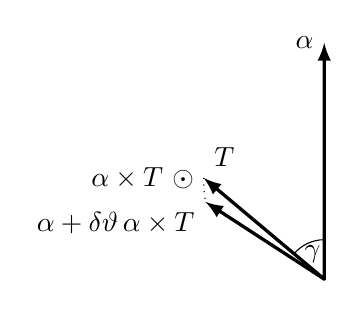
\begin{tikzpicture}
            \draw[very thick, <->, rounded corners=0.1]  (0, 3) coordinate (A) node[left] {\(\vv{\alpha}\)} -- (0, 0) coordinate (B) -- (140:2) coordinate (C) node[above right] {\(\vv{T}\)};
            \path pic[draw, "\(\gamma\)", angle eccentricity = 0.7] {angle};
            \node[left] at (C) {\(\vv{\alpha} \times \vv{T}\) \(\odot\)};
            \draw[very thick, ->] (0, 0) -- (147:1.8) node[below left] {\(\vv{\alpha} + \delta\vartheta \, \vv{\alpha} \times \vv{T}\)};
            \draw[dotted] (C) arc(180:189:2);
        \end{tikzpicture}
        \caption[Infinitesimal rotation.]{An infinitesimal rotation by \(\delta \vartheta\) of \(\vv{T}\) about \(\vv{\alpha}\) results in adding a term proportional to \(\vv{\alpha} \times \vv{T}\) to \(\vv{T}\).}
        \label{fig:infinitesimal rotation}
    \end{figure}
    
    \chapter{Further Applications}
    \section{Polynomial Invariants}
    \begin{rmk}
        This section is nonexaminable.
    \end{rmk}
    In physics we are very interested in invariant quantities, such as energy, momentum, mass, etc.
    These are all invariant under some particular symmetry and this fact can greatly simplify physics problems.
    One question that we might ask is given a number of irreducible representations how many invariant quantities can we construct?
    The simplest example of an invariant is the inner product.
    This is an invariant of a vector representation and its complex conjugate.
    
    Suppose we have an irreducible representation, which we denote by its dimension, \(\rep{X}\).
    Consider the representation \(\rep{X} \directproduct \overline{\rep{X}}\).
    We know by \cref{crl:trivial irrep in clebsch--gordan decomposition if second term is complex conjugate} that the trivial representation appears exactly once in the Clebsch--Gordan series, that is:
    \begin{equation}
        \rep{X} \directproduct \overline{\rep{X}} = 1\cdot \rep{1} \directsum \dotsb.
    \end{equation}
    The inner product corresponds to the trivial representation, \(\rep{1}\), in this decomposition.
    
    For a given group, \(G\), we can define an invariant, \(\mathcal{I}\), as an \(n\)-multilinear operator from the space of irreducible representations to \(\complex\), such that for a given group element, \(g \in G\), \(\mathcal{I}\) is unchanged if we act on each representation with itself.
    That is
    \begin{equation}
        \mathcal{I}_n = \mathcal{I}(\rep{X}_1, \dotsc, \rep{X}_n) = \mathcal{I}(\rho_1(g)\rep{X}_1, \dotsc, \rho_n(g)\rep{X}_n)
    \end{equation}
    for all \(g \in G\).
    
    The inner product then corresponds to \(\mathcal{I}_2\), it takes two values in and returns an invariant.
    More explicitly as long as \(\dim \rep{X}_a = \dim \rep{X}_b\) we define the inner product as the invariant
    \begin{equation}
        \mathcal{I}_2(\rep{X}_a, \rep{X}_b) \coloneqq \sum_{i = 1}^{\dim \rep{X}_a} (\rep{X}_a)^*_i(\rep{X}_b)_i.
    \end{equation}
    If \(\dim\rep{X}_a \ne \dim\rep{X}_b\) then no degree two invariant can be formed.
    Note that \((\rep{X}_a)_i\) here are the components of some element in the \(\rep{X}_a\) representation.
    The basis we choose isn't important since by definition of being an invariant this quantity is the same no matter what basis we choose.
    
    One way to find higher order invariants is to take Kronecker products and count how many times \(\rep{1}\) appears.
    Each occurrence leads to an invariant.
    The specific representation giving rise to \(\rep{1}\) corresponds to the degree of the associated invariant.
    
    As an example we will consider the group \(G = S_4\), and limit ourselves to irreducible representations of dimension 3 or fewer.
    The following Kronecker products can be computed:
    \begin{align}
        \rep{3}_1 \directproduct \rep{3}_1 &= \mathop{\mathrm{Sym}}(\rep{1} \directsum \rep{2} \directsum \rep{3}_1) \directsum \mathop{\mathrm{Asym}}(\rep{3}_2),\\
        \rep{3}_1 \directproduct \rep{2} &= \rep{3}_1 \directsum \rep{3}_2,\\
        \rep{3}_1 \directproduct \rep{3}_2 &= \rep{1}_1 \directsum \rep{2} \directsum \rep{3}_1 \directsum \rep{3}_2.
    \end{align}
    We restrict ourselves to considering invariants involving \(\rep{3}_1\).
    We can take \((x, y, z)\) as a generic element of this vector space associated with this representation.
    
    The antisymmetric part vanishes since it corresponds to \(\varepsilon_{ijk}x_ix_j = 0\).
    The invariants of degree at most three are
    \begin{equation}
        \mathcal{I}_2 = x^2 + y^2 + z^2, \qqand \mathcal{I}_3 = xyz.
    \end{equation}
    We have seen already that \(\mathcal{I}_2\) corresponds to the inner product.
    That this also appears for \(S_4\) is simply due to the fact that \(S_4\) is a subgroup of \(\orthogonal(3)\).
    The invariant of degree three comes from considering \(\rep{3}_1 \directproduct \rep{3}_1 \directproduct \rep{3}_1 = 1\cdot \rep{1} \directsum \dotsb\).
    
    Invariants are basis independent, as they must be to be useful.
    This follows since a similarity transformation on the representation will always affect the invariants in a definite way and we can construct them such that there is no change.
    
    A more systematic way of obtaining the degrees and interdependencies of invariants in a given representation uses the \defineindex{Molien function}, which is beyond the scope of this course.
    
    For a given degree we can construct an invariant by making a generic ansatz and averaging over the group by the \defineindex{Reynolds operator}.
    For example, consider the representation containing the vector \((x, y, z)\), again restricting ourselves to three dimensions.
    Now consider any polynomial function, \(f\), of \(x\), \(y\), and \(z\), that is \(f \in \complex[x, y, z]\).
    The following is then an invariant:
    \begin{equation}
        \mathcal{I}(x, y, z) = \frac{1}{\abs{G}} \sum_{g \in G} f(\rho(g) \circ x, \rho(g) \circ y, \rho(g) \circ z),
    \end{equation}
    where we understand \(\rho(g)\circ x\) as \(\rho(g)\ve{x}\), where \(\ve{x}\) is a unit vector in the \(x\)-direction.
    
    This operation corresponds to projection operators and will always give rise to an invariant.
    However, most of the time it will lead to 0, which is trivially invariant, unless the degree of \(f\) matches one of the degrees predicted by either the Kronecker product method or the Molien function.
    As an example consider \(f(x, y, z) = x^2\).
    From this we derive the invariant \(\mathcal{I}(x, y, z) \propto x^2 + y^2 + z^2 = \mathcal{I}_2\), with some unimportant constant of proportionality.
    
    One can think of the Clebsch--Gordan coefficient appearing in
    \begin{equation}
        \bra{c, m_c} T_{m_a}^a \ket{b, m_b} = \clebschgordan{m_c}{m_a}{m_b}{c}{a}{b} \bra{c} |T^a| \ket{b}
    \end{equation}
    as an invariant of degree three of type \(\mathcal{I}(\overline{\rep{c}}, \rep{a}, \rep{b})\).
    
    \section{Land\'e \texorpdfstring{\(g\)}{g}-Factor}
    \begin{wrn}
        In this section we choose units such that \(\hbar = 1\).
    \end{wrn}
    Consider a Hydrogen atom with a Coulomb potential.
    This system has the Hamiltonian \(H = H_0\), where \(H_0 = H_{\mathrm{Coulomb}} + H_{\text{spin-orbit}}\), where \(H_{\mathrm{Coulomb}}\) is the kinetic energy term and the Coulomb potential term, and \(H_{\text{spin-orbit}}\) is an extra term corresponding to spin-orbit coupling, the details of which are not important.
    This system exhibits spherical symmetry.
    We can break this symmetry by applying an external magnetic field.
    In this case we get a modified Hamiltonian \(H = H_0 + H'\), where \(H' = -\vv{\mu} \cdot \vv{B}\) where \(\vv{B}\) is the external magnetic field and \(\vv{\mu}\) is the dipole moment given by
    \begin{equation}
        \vv{\mu} = \frac{e}{2\pi m_{\mathrm{e}} c} (\vv{J} + \vv{S}) = \frac{e}{2\pi m_{\mathrm{e}} c} (\vv{L} + 2\vv{S}).
    \end{equation}
    Defining \(x = -eB/(2m_{\mathrm{e}} c)\) we can write the perturbing Hamiltonian as \(H' = x(L_3 + 2S_3) = x(J_3 + S_3)\), choosing the \(3\)-axis to be along the direction of the magnetic field.
    
    We assume that the energy eigenstates, \(\ket{n, l, j, m}\), of \(H_0\) are known and treat \(H'\) as a perturbation.
    The first order perturbation correction to the energy gives an extra term of the form
    \begin{equation}
        E' = \bra{n, l, j, m} H' \ket{n, l, j, m} = x(m + \expected{S_3}).
    \end{equation}
    Here we have used \(J_3\ket{n, l, j, m} = m\ket{n, l, j, m}\).
    
    Using the Wigner--Eckart theorem, and a condensed notation, \(\ket{m} = \ket{n, l, j, m}\), we have
    \begin{equation}
        \bra{m} S_i \ket{m'} = \clebschgordan{i}{m}{m'}{1}{j}{j'} \expected{\|S_1\|}, \qqand \bra{m} J_i \ket{m'} = \clebschgordan{i}{m}{m'}{1}{j}{j'} \expected{\|J_1\|}.
    \end{equation}
    Note that \(\expected{\|S_1\|}\) and \(\expected{\|J_1\|}\) are the reduced matrix elements in this condensed notation suppressing \(j\).
    What these relations tell us is that \(\bra{m}S_i\ket{m'} = a\bra{m}J_i\ket{m'}\) with
    \begin{equation}
        a \coloneqq \frac{\expected{\|S_1\|}}{\expected{\|J_1\|}}.
    \end{equation}
    Importantly \(a\) is independent of the values of \(m\) and \(m'\).
    
    We have
    \begin{equation}
        \bra{m} \vv{J}^2 \ket{m} = \sum_{m', i} \bra{m} J_i \ket{m'} \bra{m'} J_i \ket{m},
    \end{equation}
    where we have used \(\vv{J}^2 = \sum_i J_iJ_i\) and inserted the completeness relation,
    \begin{equation}
        \ident = \sum_{m'} \ket{m'}\bra{m'}.
    \end{equation}
    We similarly have
    \begin{align}
        \bra{m} \vv{J} \cdot \vv{S} \ket{m} &= \sum_{m', i} \bra{m} J_i \ket{m'}\bra{m'} S_i \ket{m}\\
        &= \sum_{m', i} \bra{m} J_i \ket{m'} a\ket{m'} J_i \ket{m}\\
        &= a\bra{m}\vv{J}^2\ket{m}\\
        &= a j(j + 1).
    \end{align}
    
    Alternatively, using \(\vv{L} = \vv{J} - \vv{S}\) we have
    \begin{equation}
        \vv{L}^2 = (\vv{J} - \vv{S})^2 = \vv{J}^2 + \vv{S}^2 - 2\vv{J}\cdot\vv{S}.
    \end{equation}
    Note that here we have used the fact that \(\vv{J}\) and \(\vv{S}\) are both from two different copies of the \(\specialUnitary(2)\) Lie algebra, and hence commute with each other, we can view both as elements of the universal enveloping algebra.
    Hence we find that
    \begin{equation}
        \bra{m} \vv{J} \cdot \vv{S} \ket{m} = -\frac{1}{2}[l(l + 1) - j(j + 1) - s(s + 1)].
    \end{equation}
    
    We can compare these two results and solve for \(a\).
    Doing so we find that
    \begin{equation}
        a = \frac{j(j + 1) + s(s + 1) - l(l + 1)}{2j(j + 1)},
    \end{equation}
    which is, as expected, independent of \(m\) and \(m'\).
    We find that
    \begin{equation}
        E'_{jlsm} = -\frac{emB}{2m_{\mathrm{e}}c} g
    \end{equation}
    where
    \begin{equation}
        g = 1 + a
    \end{equation}
    is the \define{Land\'e \(g\)-factor}\index{Lande g-factor@Land\'e \(g\)-factor} to first order in perturbation theory.
    This energy shift, \(E'\), can be added to the energy of the unperturbed Hamiltonian to lift the degeneracy.
    
    \section{Spherical Harmonics}
    The trace is linear, meaning \(\tr(A + B) = \tr(A) + \tr(B)\).
    For finite matrices we also have the cyclic property, which means in particular that \(\tr(AB) = \tr(BA)\).
    This implies that for finite matrices \(\tr(\commutator{A}{B}) = 0\).
    This cyclic property doesn't hold for operators on infinite dimensional spaces.
    The canonical commutation relation, \(\commutator{\operator{x}_i}{\operator{p}_j} = i\hbar \delta_{ij}\), has trace \(3i\hbar \ne 0\) in three spatial dimensions.
    This then implies that the position space representation is infinite dimensional.
    This shouldn't come as a surprise since the position basis is continuously labelled by \(x\).
    
    The question then is how come the representations associated with the angular momentum are finite dimensional?
    These representations are on vector spaces spanned by \(\ket{l, m}\) with \(l < n\) and \(m = -l, \dotsc, l\), making up a finite basis.
    The answer is that we can decompose the Hilbert space on the sphere, \(S^2\), into an infinite sum of finite dimensional Hilbert spaces.
    We will now investigate a basis for each of these finite dimensional Hilbert spaces.
    
    Consider \(S^2\) parametrised by the usual spherical coordinates \((\vartheta, \varphi)\).
    Note that we keep \(r = 1\) fixed and so this is a two-dimensional manifold embedded in 3-dimensional space.
    A state \(\ket{\vartheta, \varphi}\) obeys the completeness and orthogonality relations
    \begin{align}
        \ident_{S^2} &= \int \dl{\Omega} \, \ket{\vartheta, \varphi}\bra{\vartheta, \varphi},\\
        \braket{\vartheta, \varphi}{\vartheta', \varphi'} &= \delta(\varphi - \varphi')\delta(\cos\vartheta - \cos\vartheta').
    \end{align}
    Note that \(\dl{\Omega} = \sin\vartheta \dd{\varphi}\dd{\vartheta}\) is a solid angle element, so
    \begin{equation}
        \int_{S^2}\dd{\Omega} = \int_0^{2\pi} \dd{\varphi} \int_{0}^{\vartheta} \dd{\vartheta} \, \sin\vartheta = \int_0^{2\pi} \dd{\varphi} \int_{-1}^{1} \dl{(\cos \vartheta)}.
    \end{equation}

    We can decompose the Hilbert space \(\hilbert_{S^2} = \spn\{\ket{\vartheta, \varphi}\}\), as a direct sum of the Hilbert spaces \(\hilbert_{l} = \spn\{\ket{l, m} \mid m = -l, \dotsc, l\}\).
    Clearly
    \begin{equation}
        \dim\hilbert_l = \abs{\spn\{\ket{l, m} \mid m = -l, \dotsc, l\}} = \abs{\{-l, \dotsc, l\}} = 2l + 1.
    \end{equation}
    We then have
    \begin{equation}
        \hilbert_{S^2} = \bigoplus_{l = 0}^{\infty} \hilbert_l.
    \end{equation}
    We can rewrite the completeness and orthogonality relations for \(\hilbert_{S^2}\) in terms of its decomposition, giving
    \begin{align}
        \ident_{S^2} &= \sum_{l = 0}^{\infty}\sum_{m = -l}^{l} \ket{l, m}\bra{l, m},\\
        \braket{l, m}{l', m'} &= \delta_{ll'}\delta_{mm'}.
    \end{align}
    
    \begin{dfn}{Spherical Harmonic}{}
        We define the \define{spherical harmonics}\index{spherical harmonic}, \(Y_{lm}\colon S^2 \to \complex\), as the projection of the state \(\ket{l, m}\) onto \(\ket{\vartheta, \varphi}\):
        \begin{equation}
            Y_{lm}(\vartheta, \varphi) \coloneqq \braket{\vartheta, \varphi}{l, m}.
        \end{equation}
    \end{dfn}
    
    \begin{lma}{}{}
        The following orthogonality relations hold for the spherical harmonics:
        \begin{align}
            \int Y_{l'm'}^*(\vartheta, \varphi) Y_{lm}(\vartheta, \varphi) \dd{\Omega} &= \delta_{ll'}\delta_{mm'},\\
            \sum_{l = 0}^{\infty} \sum_{m = -l}^{l} Y_{lm}(\vartheta, \varphi)Y_{lm}^*(\vartheta', \varphi') &= \delta(\varphi - \varphi')\delta(\cos\vartheta - \cos\vartheta').
        \end{align}
        \begin{proof}
            We start with the orthogonality relation for \(\ket{l, m}\):
            \begin{equation}
                \braket{l, m}{l', m'} = \delta_{ll'}\delta_{mm'}.
            \end{equation}
            We then insert the completeness relation for \(\ket{\vartheta, \varphi}\):
            \begin{equation}
                \ident_{S^2} = \int \dl{\Omega} \, \ket{\vartheta, \varphi}\bra{\vartheta, \varphi}.
            \end{equation}
            This gives
            \begin{equation}
                \int\dl{\Omega} \braket{l, m}{\vartheta, \varphi}\braket{\vartheta, \varphi}{l', m'} = \delta_{ll'}\delta_{mm'}.
            \end{equation}
            Now we use \(\braket{l, m}{\vartheta, \varphi} = \braket{\vartheta, \varphi}{l, m}^*\) and the definition of the spherical harmonics as \(Y_{lm}(\vartheta, \varphi) \coloneqq \braket{\vartheta, \varphi}{l, m}\) to get
            \begin{equation}
                \int\dl{\Omega} Y_{lm}^*(\vartheta, \varphi)Y_{l'm'}(\vartheta, \varphi) = \delta_{ll'}\delta_{mm'}.
            \end{equation}
            Exchanging which symbols are primed we get the desired result.
            
            Next we start with the orthogonality relation for \(\ket{\vartheta, \varphi}\):
            \begin{equation}
                \braket{\vartheta, \varphi}{\vartheta', \varphi'} = \delta(\varphi - \varphi')\delta(\cos\vartheta - \cos\vartheta').
            \end{equation}
            We then insert the completeness relation for \(\ket{l, m}\):
            \begin{equation}
                \ident_{S_2} = \sum_{l = 0}^{\infty} \sum_{m = -l}^l \ket{l, m}\bra{l, m}.
            \end{equation}
            This gives
            \begin{equation}
                \sum_{l = 0}^{\infty} \sum_{m = -l}^{l} \braket{\vartheta, \varphi}{l, m}\braket{l, m}{\vartheta', \varphi'} = \delta(\varphi - \varphi')\delta(\cos\vartheta - \cos\vartheta').
            \end{equation}
            Again using \(\braket{l, m}{\vartheta', \varphi'} = \braket{\vartheta', \varphi'}{l, m}^*\) and the definition of the spherical harmonics as \(Y_{lm}(\vartheta, \varphi) \coloneqq \braket{\vartheta, \varphi}{l, m}\) we get
            \begin{equation}
                \sum_{l = 0}^{\infty} \sum_{m = -l}^{l} Y_{lm}(\vartheta, \varphi) Y_{lm}^*(\vartheta', \varphi') = \delta(\varphi - \varphi')\delta(\cos\vartheta - \cos\vartheta').
            \end{equation}
        \end{proof}
    \end{lma}
    
    For \(l = 0, 1\), using the Condon--Shortley phase convention, the spherical harmonics are given by
    \begin{alignat}{4}
        Y_{00}(\vartheta, \varphi) &= \frac{1}{2}\sqrt{\frac{1}{\pi}},\\
        Y_{10}(\vartheta, \varphi) &= \frac{1}{2}\sqrt{\frac{3}{\pi}} \cos\vartheta &&= \frac{1}{2}\sqrt{\frac{3}{\pi}} \frac{z}{r}, \label{eqn:Y10} \\
        Y_{1,{-1}}(\vartheta, \varphi) &= \frac{1}{2}\sqrt{\frac{3}{2\pi}}\e^{-i\varphi}\sin\vartheta &&= \frac{1}{2}\sqrt{\frac{3}{2\pi}} \frac{x - iy}{r},\\
        Y_{11}(\vartheta, \varphi) &= -\frac{1}{2}\sqrt{\frac{3}{2\pi}}\e^{i\varphi}\sin\vartheta &&= -\frac{1}{2}\sqrt{\frac{3}{2\pi}} \frac{x + iy}{r}.
    \end{alignat}
    In general the \(\varphi\) dependence of \(Y_{lm}\) only appears through a \(\e^{im\varphi}\) term and the \(\vartheta\) dependence appears through trigonometric terms \(\sin\vartheta\) and \(\cos\vartheta\), which occur with maximum power \(l\).
    This follows from the fact that we can write the spherical harmonics as
    \begin{equation}
        Y_{lm}(\vartheta, \varphi) = \sqrt{\frac{(2l + 1)}{4\pi}\frac{(l - m)!}{(l + m)!}} P_{lm}(\cos\vartheta)\e^{im\varphi}.
    \end{equation}
    Here \(P_{lm}\) are the \define{associated Legendre polynomials}\index{associated Legendre polynomial}, which are polynomials of order \(l\).
    A useful property of the spherical harmonics is that
    \begin{equation}
        Y_{l,{-m}} = (-1)^mY_{lm}^*.
    \end{equation}
    
    The quadratic Casimir operator, \(L^2\), on \(S^2\) is given by
    \begin{equation}
        \int \dl{\Omega} \bra{\vartheta', \varphi'} \left( -\frac{L^2}{\hbar^2} \right) \ket{\vartheta, \varphi} = \frac{1}{\sin^2\vartheta}\diffp[2]{}{\varphi} + \frac{1}{\sin \vartheta} \diffp{}{\vartheta}\left( \sin\vartheta \diffp{}{\vartheta} \right).
    \end{equation}
    This corresponds to the Laplacian, \(\laplacian[S^2]\), on \(S^2\).
    We therefore have that
    \begin{equation}
        \laplacian[S^2]Y_{lm} = -\frac{L^2}{\hbar^2}Y_{lm} = -l(l + 1)Y_{lm}.
    \end{equation}
    Which follows since we know that the action of the quadratic Casimir, \(L^2\), for \(\specialUnitary(2)\) is to multiply by a factor of \(l(l + 1)\).
    It makes sense that this should be the Casimir.
    First, the Laplacian is invariant under rotations, and it is of second order, as a quadratic Casimir must be.
    Solutions to Laplace's equation are called harmonic functions, which explains the name \enquote{spherical harmonics}, they are harmonic functions on the sphere.
    
    \subsection{Application to \texorpdfstring{\(\reals^3 \isomorphic \reals^+ \directproduct S^2\)}{R3 isomorphic R+ x S2}}
    We can decompose three-dimensional Euclidean space, \(\reals^3\), into a product of the non-negative real numbers, \(\reals^+ \coloneqq \{r \in \reals \mid r \ge 0\}\), and the sphere, \(S^2\):
    \begin{equation}
        \reals^3 \isomorphic \reals^+ \directproduct S^2.
    \end{equation}
    This is most obvious when working in spherical polar coordinates, where we associate the radial coordinate \(r\) with \(\reals^+\) and the angular components, \((\vartheta, \varphi)\), with \(S^2\).
    Since the spherical harmonics are a complete set of functions on \(S^2\) we can express any\footnote{Well, any function of interest in physics.} function, \(f \colon \reals^3 \to \complex\) as
    \begin{equation}
        f(x, y, z) = \sum_{n = 1}^{\infty} \sum_{l = 0}^{n - 1} \sum_{m = -l}^{l} u_{nlm}(r) Y_{lm}(\vartheta, \varphi)
    \end{equation}
    where \(u_{nlm} \colon \reals^+ \to \complex\) and \(Y_{lm}\colon S^2 \to \complex\) are the spherical harmonics.
    
    The Laplacian in spherical coordinates is
    \begin{equation}
        \laplacian[\reals^3] = \frac{1}{r^2} \diffp{}{r}\left( r^2 \diffp{}{r} \right) + \laplacian[S^2].
    \end{equation}
    This is used, for example, to express the Schrödinger equation in spherical coordinates.
    
    \begin{dfn}{Solid Harmonics}{}
        The \define{solid harmonics}\index{solid harmonic} are the functions \(\mathcal{Y}_{lm} \colon \reals^3 \to \complex\) defined by
        \begin{equation}
            \mathcal{Y}_{lm}(r, \vartheta, \varphi) \coloneqq r^{l} Y_{lm}(\vartheta, \varphi).
        \end{equation}
    \end{dfn}
    
    The solid harmonics are solutions to Laplace's equation in \(\reals^3\), that is
    \begin{equation}
        \laplacian[\reals^3] \mathcal{Y}_{lm} = 0.
    \end{equation}
    These are particularly useful when we have a spherically symmetric potential, which we can write as \(V(r)\), that is as a function of only the distance from the origin, with no angular dependence.
    In this case the solution doesn't depend on the magnetic quantum number, \(m\), since \(m\) singles out a direction in space, defining the \(L_3\) operator as the angular momentum along a particular axis.
    We therefore reduce \(u_{nlm}\) to \(u_{nl}\) and the Schrödinger equation in three dimensions reduces to a Schrödinger equation in one dimension for the radial component:
    \begin{equation}
        \left( -\frac{\hbar^2}{2m}\frac{1}{r^2}\diffp{}{r}(r^2\diffp{}{r}) + V_l^{\mathrm{eff}}(r) \right) u_{nl}(r) = E_{nl}u_{nl}.
    \end{equation}
    Here \(V_l^{\mathrm{eff}}\) is the effective potential
    \begin{equation}
        V_l^{\mathrm{eff}}(r) \coloneqq V(r) + \frac{\hbar^2}{2m}\frac{l(l + 1)}{r^2}.
    \end{equation}
    Note that we are now restricting \(u_{nl}\) to be eigenfunctions of the Schrödinger equation, rather than an arbitrary complete set of functions on \(\reals^+\) as they originally were.
    
    \subsection{Why \texorpdfstring{\(S^2\)}{S2}?}
    Why is it that \(S^2\) appears as the manifold of interest here.
    We are considering \(\specialOrthogonal(3)\) symmetry, and the manifold of \(\specialOrthogonal(3)\) is \(\mathbb{RP}^3\), that is \(S^3\) with antipodal points associated.
    So, why is this not the manifold that we are considering?
    
    Consider an arbitrary vector in \(\reals^3\).
    We may as well define a coordinate system such that this arbitrary vector is \(v = (1, 0, 0)\).
    We can act on this vector using \(\specialOrthogonal(2)\) to act on the \(y\) and \(z\) components, that is we act on it with \(\ident_1 \directproduct R\) with \(R \in \specialOrthogonal(2)\).
    So
    \begin{equation}
        \ident_1 \directproduct R = 
        \begin{pmatrix}
            1 & 0 & 0\\
            0 & \hphantom{-}\cos\vartheta & \sin\vartheta\\
            0 & -\sin\vartheta & \sin\vartheta
        \end{pmatrix}
        .
    \end{equation}
    The interpretation of this is of course as a rotation about \(v = (1, 0, 0)\).
    
    The fact that our arbitrary vector is invariant under this operation means we have some redundancy, and to get rid of it we mod out by \(\specialOrthogonal(2)\).
    Doing so the relevant manifold is
    \begin{equation}
        \specialOrthogonal(3) / \specialOrthogonal(2) \isomorphic S^2.
    \end{equation}
    Note that this is \emph{not} a group manifold since \(\specialOrthogonal(2)\) is \emph{not} normal in \(\specialOrthogonal(3)\).
    
    \chapter{Selection Rules}
    \section{Parity Selection}
    Recall that we defined \defineindex{parity symmetry} as
    \begin{equation}
        \Psym \circ (t, x, y, z) = (t, -x, -y, -z), \qquad \Psym \circ \vv{r} = -\vv{r}.
    \end{equation}
    Until 1956 it was believed that parity was strictly conserved in all interactions.
    In 1956 theorists posited that parity conservation may be violated in weak interactions.
    Experiments and further development of the theory found that parity is in fact maximally violated in weak interactions.
    The weak force ignores so called \enquote{right handed particles} and acts only on \enquote{left handed particles}.
    For this reason many attach an \(\mathrm{L}\) subscript to the symmetry group of the weak force, \(\specialUnitary(2)_{\mathrm{L}}\).
    In practice the weak force is, well, weak, and can be neglected in many strong and electromagnetic interactions, so the parity is still usually a good quantum number.
    
    By allowing parity violation we effectively extend the symmetry group from \(\specialOrthogonal(3)\) to \(\orthogonal(3)\), since we can write elements of \(\orthogonal(3)\) as a reflection times an element of \(\specialOrthogonal(3)\), with the reflection corresponding to swapping the parity.
    We implement the parity transformation as a unitary transformation, \(U(\Psym)\).
    Further, reversing parity and then reversing back cannot change the physics, and hence we must have that \(U(\Psym)^2 = \e^{i\eta}\ident\), so that upon doubly reversing the parity the only effect is a phase change.
    Often we are free to choose this phase factor, so in which case we usually choose \(\eta = 0\), corresponding to \(U(\Psym) = \pm\ident\).
    
    Given a state \(\ket{l, m}\) the parity transformation is
    \begin{equation}
        U(\Psym)\ket{l, m} = (-1)^l\ket{l, m}
    \end{equation}
    for \(l \in \naturals\).
    This can be inferred from the parity transformation properties of the spherical harmonics:
    \begin{equation}
        \Psym \circ Y_{lm}(\vartheta, \varphi) = Y_{lm}(\pi - \vartheta, \varphi + \pi) = (-1)^lY_{lm}(\vartheta, \varphi).
    \end{equation}
    This can be seen by either thinking about the coordinates \((r, \vartheta, \varphi)\) being inverted through the origin, or algebraically by changing \(x \to -x\), \(y \to -y\), and \(z \to -z\) in the equations \(\vartheta = \arctan(\sqrt{x^2 + y^2}/z)\) and \(\varphi = \arctan(y/x)\).
    
    Suppose we have  a transition governed by the operator \(X\).
    The parity of the operator is \(\eta_X\), which is given by \(U(\Psym) X U(\Psym)^\hermit = (-1)^{\eta_X}X\), or equivalently \(X = (-1)^{\eta_X}U(\Psym)^\hermit XU(\Psym)\).
    We then have the selection rule that
    \begin{equation}
        \bra{l, m} X \ket{l', m'} \ne 0
    \end{equation}
    only if \(l + l' + \eta_X\) is even, since we have
    \begin{align}
        \bra{l, m} X \ket{l', m'} &= \bra{l, m} (-1)^{\eta_X} U(\Psym)^\hermit XU(\Psym) \ket{l', m'}\\
        &= (-l)^{l + l' + \eta_X} \bra{l, m} X \ket{l', m'}.
    \end{align}
    Hence we have \((-1)^{l + l' + \eta_X} = 1\), which implies \(l + l' + \eta_X\) is even.
    Note that if \(X\) is a tensor operator we also have the selection rules that \(\abs{j_1 - j_2} \le J \le j_1 + j_2\), and \(M = m_1 + m_2\).
    
    Common examples of operators with definite parity are the position, \(\vv{x}\), momentum, \(\vv{p}\), angular momentum, \(\vv{L}\), electric field, \(\vv{E}\), and magnetic field, \(\vv{B}\).
    Of these \(\vv{x}\), \(\vv{p}\), \(\vv{E}\) are proper vectors, so have parity \(\eta_{\vv{x}} = \eta_{\vv{p}} = \eta_{\vv{E}} = 1\), whereas \(\vv{L}\) and \(\vv{B}\) are \define{pseudo-vectors}\index{pseudo-vector}, meaning they change by a sign under a parity transformation, and hence \(\eta_{\vv{L}} = \eta_{\vv{B}} = 0\).
    
    It is easy enough to show the pseudo-vector nature of \(\vv{L}\), since we know that \(\vv{L} = \vv{x} \times \vv{p}\), so
    \begin{equation}
        \Psym\circ \vv{L} = \Psym \circ (\vv{x} \times \vv{p}) = (\Psym\circ\vv{x})\times(\Psym\circ\vv{p}) = (-\vv{x}) \times (-\vv{p}) = \vv{x} \times \vv{p} = \vv{L}.
    \end{equation}
    In fact the cross product of two vectors is always a pseudo-vector.
    Similarly the cross product of two pseudo-vectors is a pseudo-vector, and the cross product of a pseudo-vector and vector is a vector.
    This is the logic that means \(\vv{B}\) is a pseudo vector since we have that \(\vv{F} = q\vv{E} + q\vv{v}\times\vv{B}\), and since \(\vv{F}\) is a proper vector and so is \(\vv{v}\) we must have that \(\vv{B}\) is a pseudo-vector.
    
    Each particle has an intrinsic parity.
    Bosons have the same intrinsic parity as their antiparticles, whereas fermions have the opposite parity to their antiparticles.
    This is a result of causality in QFT.
    The angular momentum of a particle is a quantum number, \(J\).
    It is also possible for the intrinsic parity to have this pseudo property.
    If we are allowing for this then we label the particles with the quantum number \(J^\pm\), with \(-\) for when \(\eta\) is odd and \(+\) when \(\eta\) is even.
    For example, the \(\uprho\)-meson (\(\mathrm{u}\bar{\mathrm{d}}\)) is a vector meson, meaning \(S = J = 1\), and the \(\mathrm{A}_1\)-meson (\(\bar{\mathrm{u}}\mathrm{d}\)) is also a vector meson.
    However, the \(\uprho\)-meson has negative parity, so is \(1^{-}\), whereas the \(\mathrm{A}_1\)-meson has positive parity, so is \(1^{+}\).
    We say that the \(\mathrm{A}_1\)-meson is a pseudo-vector particle.
    
    When we are only interested in computing transitions between like particles, for example, an electron going from one energy level to another, the parity cancels from both sides of the equation.
    For this reason we often ignore parity when we are doing quantum mechanics.
    When we are doing particle physics, such as QFT, however, we often consider cases where we generate new particles, potentially with different parities.
    A general example would be the decay \(A \to B + C\).
    In this case the parity of the final state is the sum of the intrinsic parities and the angular momentum, \(\eta_{\mathrm{tot}} = \eta_B + \eta_C + \eta_L\).
    If \(A\) has definite parity and the interaction conserves parity (i.e. it is not a weak interaction) then we must have that \((-1)^{\eta_A} = (-1)^{\eta_{\mathrm{tot}}}\).
    
    \section{Superselection}
    Superselection rules generalise selection rules.
    Selection rules refer to a particular Hamiltonian which is such that only certain transitions between states occur with non-zero probability.
    Superselection rules state that certain matrix elements vanish for \emph{all} observables.
    That is given the states \(\ket{\psi}\) and \(\ket{\varphi}\) ew say these states are separated by a \defineindex{superselection rule} if
    \begin{equation}
        \bra{\psi} O \ket{\varphi} = 0
    \end{equation}
    for all observables \(O\).
    
    This means that a relative phase between \(\ket{\psi}\) and \(\ket{\varphi}\) is unobservable, and hence there is no coherent state of the form \(a\ket{\psi} + b\ket{\varphi}\).
    
    Notice that we can always define an Hermitian operator \(X \coloneqq \ket{\psi}\bra{\varphi} + \ket{\varphi}\bra{\psi}\), and clearly
    \begin{equation}
        \bra{\psi}X\ket{\varphi} = \braket{\psi}{\psi}\braket{\varphi}{\varphi} + \braket{\psi}{\varphi}\braket{\varphi}{\psi} = 1 \ne 0.
    \end{equation}
    What this means is that the presence of superselection rules really means that not all Hermitian operators are valid observables.
    That is the space of observables is a strict subset of the space of Hermitian operators in the presence of superselection rules.
    
    An example of a superselection is the fermionic/bosonic nature of a particle.
    Suppose that \(\ket{1/2}\) is a fermionic state, and \(\ket{1}\) is a bosonic state.
    We could, at least mathematically in the Hilbert space, define a vector \(\ket{\psi} = a\ket{1/2} + b\ket{1}\), however, this doesn't correspond to a physically meaningful state.
    This is because upon a \(2\pi\) rotation, due to some operator, \(U(2\pi)\), a fermionic state will pick up a negative sign, but a bosonic state won't, so
    \begin{equation}
        U(2\pi)\ket{\psi} = -a\ket{1/2} + b\ket{1}.
    \end{equation}
    Clearly this doesn't make any physical sense, since the relative phase between \(a\) and \(b\) changes by \(\pi\) upon rotation.
    
    Another example is conserved charge.
    It doesn't make sense to write, for example, \(\ket{\psi} = \ket{\Pe} + \ket{\APe}\), since these transform under complex conjugates representations, and so pick up opposite phases when transforming.
    The only time that this isn't a problem is if the representation is real, but this corresponds to the particle being neutral.
    
    \section{Electric Dipole}
    Consider an extended charge distribution, \(\rho\).
    To first order in the multipole expansion we can write the Hamiltonian in an external field, \(\vv{E}\), as
    \begin{equation}
        H = H_0 + H'
    \end{equation}
    where \(H_0\) is a Coulomb term and \(H' = -\vv{d} \cdot \vv{E}\), where \(\vv{d}\) is the electric dipole moment, given by
    \begin{equation}
        \vv{d} \coloneqq \int \rho(\vv{x}) \vv{x} \dd{^3x}.
    \end{equation}
    Importantly \(\vv{d}\) transforms the same as \(\vv{x}\), due to the factor of \(\vv{x}\) in the definition.
    We know that \(\vv{x}\) is a \(j = 1\) tensor operator (that is, a vector) and hence the Wigner--Eckart theorem applies, as do the associated selection rules.
    
    For simplicity we consider the case of an external field aligned along the \(z\)-axis, so \(\vv{E} = E_z\ve{z}\).
    It follows from this that \(H' \propto z\) since
    \begin{equation}
        H' = -\int \rho(\vv{x}) \vv{x} \dd{^3x} \cdot \ve{E} = -E_z \int \rho(\vv{x}) \vv{x} \cdot \ve{z} \dd{^3x} = -E_z \int \rho(\vv{x}) z \dd{^3x}.
    \end{equation}
    So \(H'\) transforms like \(z\).
    Looking at the spherical harmonics in \cref{eqn:Y10} we see that
    \begin{equation}
        Y_{10} \propto \frac{z}{r}.
    \end{equation}
    Considering the definition of the solid harmonics as \(\mathcal{Y}_{lm} = r^lY_{lm}\) we see that
    \begin{equation}
        \mathcal{Y}_{10} \propto z.
    \end{equation}
    So \(H' \propto \mathcal{Y}_{10}\).
    
    Applying the Wigner--Eckart theorem we then have
    \begin{equation}
        \bra{l,m} H' \ket{l',m'} \propto \bra{l,m}\mathcal{Y}_{10}\ket{l',m'} = \clebschgordan{m}{0}{m'}{l}{1}{l'} \bra{l} |\mathcal{Y}_1 \ket{l'}.
    \end{equation}
    We know that the Clebsch--Gordan coefficient, \(\clebschgordan{M}{m_1}{m_2}{J}{j_1}{j_2}\), is non-zero only if \(M = m_1 + m_2\), so we must have \(m = m'\), and if \(\abs{j_1 - j_2} \le J \le j_1 + j_2\), which means that we must have \(\Delta l \coloneqq \abs{l - l'} \le 1\).
    Further \(\clebschgordan{m}{0}{m'}{0}{1}{0} = 0\) for all allowed values of \(m\) and \(m'\), which is just \(m = m' = 0\).
    This means we cannot have \(l = l' = 0\).
    
    Further considering parity selection rules since \(\eta_{\vv{x}} = 1\), and \(H'\) transforms like \(\vv{x}\), so has the same parity which means we must have \(l + l' + \eta_{\vv{x}} = l + l' + 1\) even.
    Hence we cannot have \(l - l' = 0\), since if this is the case then \(l + l' + 1 = 2l + 1\), which is odd for all integer \(l\).
    So \(\Delta l \ne 0\).
    Hence we have the selection rules
    \begin{equation}
        m = m', \qqand \Delta l = \abs{l - l'} = 1.
    \end{equation}
    
    \section{Pauli's Hydrogen Atom}
    \begin{wrn}
        In this section we use units such that \(c = \hbar = 1\).
    \end{wrn}
    Shortly after Schrödinger solved his equation for the hydrogen atom Pauli did so using group theory and a hidden \(\specialUnitary(2) \directproduct \specialUnitary(2)\) symmetry.
    The energy levels of the hydrogen atom are given by
    \begin{equation}
        E_n = -\frac{m_{\mathrm{e}}e^4}{2} \frac{1}{n^2}.
    \end{equation}
    Importantly there is no \(l\) dependence.
    This means that for each value of the principal quantum number, \(n\), we have \(l = 0, \dotsc, n - 1\), which means the total degeneracy is
    \begin{equation}
        \sum_{l = 0}^{n - 1} (2l + 1) = 2\sum_{l = 0}^{n - 1}l + \sum_{l = 0}^{n - 1} = 2\frac{n - 1}{2}n + n = n^2.
    \end{equation}
    Note that the \(2l + 1\) term is due to degeneracy in \(m\), which runs from \(-l\) to \(l\), so takes on \(2l + 1\) values for fixed \(l\).
    
    The degeneracy in \(m\) is expected, since we have a spherically symmetric potential, and \(m\) picks out a direction.
    The fact that we have no \(l\) dependence suggests that there is some further symmetry which we are missing.
    Pauli used the fact that there is a conserved vector, \(\vv{A}\), with components
    \begin{equation}
        A_i = \varepsilon_{ijk}p_jL_k - me^2\frac{x_i}{r},
    \end{equation}
    which is conserved in a spherically symmetric system in classical mechanics.
    This is known as the \defineindex{Laplace--Runge--Lenz vector}.
    In quantum mechanics there is a related quantity given by symmetrisation:
    \begin{equation}
        A_i = \varepsilon_{ijk}p_jL_k - me^2\frac{x_i}{r} - ip_i
    \end{equation}
    Note that this is an operator in quantum mechanics.
    It can be shown that the following hold:
    \begin{gather}
        \vv{L} \cdot \vv{A} = \vv{A} \cdot \vv{L} = 0,\\
        \commutator{L_i}{A_j} = i\varepsilon_{ijk}A_k,\\
        \commutator{H}{A_i} = 0, \qwhere H = \sum_i\frac{p_i^2}{2m} - \frac{e^2}{r}.
    \end{gather}
    The second of these means that \(A_i\) is a \(j = 1\) vector operator.
    The third means that \(\vv{A}\) is conserved.
    
    By Noether's theorem we can identify from this conservation law that there must be a hidden symmetry.
    To find this symmetry we make some new definitions and extract a Lie algebra.
    Start by defining
    \begin{equation}
        \tilde{A}_i \coloneqq \frac{A_i}{\sqrt{-2mH}}.
    \end{equation}
    Note that for a bound state the total energy is negative, so we take the minus sign in the root to keep \(\tilde{A}_i\) real.
    It can then be shown that
    \begin{equation}
        \liebracket{\tilde{A}_i}{\tilde{A}_j} = i\varepsilon_{ijk}\tilde{A}_k.
    \end{equation}
    This shows that \(\tilde{A}_i\) are the generators of a \(\specialUnitaryLie(2)\) Lie algebra.
    We then define \(X_i^{\pm} \coloneqq (L_i \pm \tilde{A}_i) / 2\).
    From this the commutation relation
    \begin{equation}
        \liebracket{X_i^{\pm}}{X_j^{\pm}} = i\varepsilon_{ijk}X_k^{\pm}
    \end{equation}
    follows, since both \(L_i\) and \(A_i\) individually satisfy the requirements of a \(\specialUnitaryLie(2)\) Lie algebra, and since \(\vv{L} \cdot \vv{A} = \vv{A} \cdot \vv{L} = 0\) cross terms vanish.
    
    The result is that we identify an overall \(\specialUnitary(2) \directproduct \specialUnitary(2)\) symmetry, corresponding to the two copies of the \(\specialUnitaryLie(2)\) Lie algebra, spanned by \(X_i^+\) and \(X_i^-\) respectively.
    We can think of one copy as resulting from rotational symmetry and the second from the symmetry associated with conservation of \(\vv{A}\).
    
    One question we may want to ask is what are the Casimir operators of these two Lie algebras are.
    The fact that \(\vv{L} \cdot \vv{A} = \vv{A} \cdot \vv{L} = 0\) means that the two Casimir operators are actually the same, in particular the quadratic Casimir is
    \begin{equation}
        C_2^+ = (X^+)^2 = (X^-)^2 = C_2^- = C_2.
    \end{equation}
    We can parametrise this Casimir by \(C_2 = x(x + 1)\) with \(x = 0, 1/2, 1, 3/2, \dotsc\).
    
    From this it is possible to show that
    \begin{equation}
        A_iA_i = 2mH(L_iL_i + 1) + m^2e^4.
    \end{equation}
    Dividing through by \(-2mH\) and solving for \(H\) we get
    \begin{equation}
        H = -\frac{me^4/2}{L_iL_i + \tilde{A}_i\tilde{A}_i + 1} = -\frac{me^4/2}{4C_2 + 1} = -\frac{me^4/2}{(2x + 1)^2}
    \end{equation}
    for \(x = 0, 1/2, 1, 3/2, \dotsc\).
    The second equality follows using \(L_i = X_i^+ + X_i^-\).
    Counting the degeneracy of the states corresponds to counting the states in the direct product representation \(\rho_{j = x} \directproduct \rho_{j = x}\), which has \((2x + 1)^2\) states.
    Comparing this with our initial work in this section we identify the principal quantum number \(n = 2x + 1\).
    
    Pauli's approach here was to write the Hamiltonian in terms of two Casimir operators (which just happen to be equal).
    That this is possible is not an accident.
    In the absence of spin we need three quantum numbers to describe a state, say \(\{x_1, x_2, x_3\}\), \(\{p_1, p_2, p_3\}\), or as is most common when talking about the hydrogen atom, \(\{n, l, m\}\).
    Spherical symmetry guarantees that \(m\) doesn't appear in the final result, and hence we are reduced to two quantum numbers.
    This means that a rank two symmetry, with two Casimirs, is sufficient to obtain solutions based solely on symmetry.
    In order to include the effects of spin, as well as other relativistic corrections, we still need to solve Schrödinger's equation.
    
    
    %   Appdendix
    \appendixpage
    \begin{appendices}
        \chapter{Mathematical Preliminaries}
\section{Basic Mathematics}
\subsection{Notation}
\begin{ntn}{Number Sets}{}
    The set of natural numbers is
    \begin{equation}
        \naturals \coloneqq \{0, 1, 2, \dotsc\}.
    \end{equation}
    Note that the inclusion of zero in \(\naturals\) is subject to debate.
    The set of integers is denoted
    \begin{equation}
        \integers \coloneqq \{\dotsc, -2, -1, 0, 1, 2, \dotsc\}.
    \end{equation}
    The set of positive integers is denoted
    \begin{equation}
        \positiveintegers \coloneqq \{1, 2, \dotsc\}.
    \end{equation}
    The set of rational numbers is denoted
    \begin{equation}
        \rationals \coloneqq \{p/q \mid p, q \in \integers \text{ and } q \ne 0\}.
    \end{equation}
    The set of real numbers is denoted \(\reals\), and the set of complex numbers \(\complex\).
    The set of \emph{all} quaternions (as opposed to the quaternion group of order 8) is denoted \(\quaternions\).
\end{ntn}

\begin{ntn}{Sphere}{}
    The unit sphere in \(n + 1\) dimensions is
    \begin{equation}
        S^n \coloneqq \{\vv{x} \in \reals^{n+1} \mid x_1^2 + \dotsb x_{n+1}^2 = 1\}.
    \end{equation}
    Note that \(S^n\) is an \(n\)-dimensional manifold, which we view as embedded in \((n + 1)\)-dimensional Euclidean space, \(\reals^{n+1}\).
    
    What we normally call the circle is \(S^1\) and what we normally call the sphere is \(S^2\).
\end{ntn}

\begin{ntn}{Sets of Matrices}{}
    We denote the set of \(m \times n\) matrices with entries in \(\field\) (which is usually a field and usually \(\reals\) or \(\complex\)) by \(\matrices[m]{n}{\field}\).
    
    We denote the set of square \(n \times n\) matrices with entries in \(\field\) by \(\matrices{n}{\field}\).
    
    We denote the set of invertible \(n\times n\) square matrices over \(\field\), called the general linear group, by
    \begin{equation}
        \generalLinear(n, \field) = \{A \in \matrices{n}{\field} \mid \det A \ne 0\}.
    \end{equation}
    If \(\field\) is evident from context we may simply write \(\generalLinear(n)\).
    If \(V\) is an \(n\)-dimensional vector space over \(\field\) then we may also write this set as \(\generalLinear(V)\).
\end{ntn}

\begin{ntn}{Einstein Summation Convention}{}
    When two identical indices appear in the same term then they are summed over, for example,
    \begin{equation}
        x_iy_i = \sum_{i} x_iy_i.
    \end{equation} 
\end{ntn}

\subsection{Definitions}
\begin{dfn}{Function Types}{}
    Let \(\varphi \colon A \to B\).
    Then \(\varphi\) is 
    \begin{itemize}
        \item \defineindex{injective} if for all \(a, a' \in A\) \(\varphi(a) = \varphi(a')\) implies \(a = a'\),
        \item \defineindex{surjective} if for all \(b \in B\) there exists \(a \in A\) such that \(\varphi(a) = b\), and
        \item \defineindex{bijective} if \(\varphi\) is both injective and surjective.
    \end{itemize}
    A function is invertible if and only if it is bijective.
\end{dfn}

\begin{figure}
    \begin{subfigure}[t]{0.45\textwidth}
        \centering
        \tikzsetnextfilename{injective-function}
        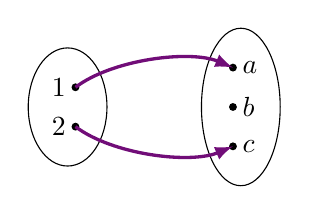
\begin{tikzpicture}
            \foreach \y in {-0.5, 0, 0.5} {
                \fill (2, \y) circle [radius = 0.05cm];
            }
            \foreach \y in {-0.25, 0.25} {
                \fill (0, \y) circle [radius = 0.05cm];
            }
            \node [right] at (2, -0.5) {\(c\)};
            \node [right] at (2, 0) {\(b\)};
            \node [right] at (2, 0.5) {\(a\)};
            \node [left] at (0, -0.25) {\(2\)};
            \node [left] at (0, 0.25) {\(1\)};
            \draw (-0.1, 0) circle [x radius = 0.5, y radius = 0.75];
            \draw (2.1, 0) circle [x radius = 0.5, y radius = 1];
            
            \draw [very thick, highlight, ->] (0, 0.25) to[bend left, looseness=0.75] (2, 0.5);
            \draw [very thick, highlight, ->] (0, -0.25) to[bend right, looseness=0.75] (2, -0.5);
        \end{tikzpicture}
        \caption{An injective function, \(f \colon \{1, 2\} \to \{a, b, c\}\). Note that \(f(x) \ne b\) for any \(x \in \{1, 2\}\) and so the function fails to be surjective.}
    \end{subfigure}
    \hspace{0.05\textwidth}
    \begin{subfigure}[t]{0.45\textwidth}
        \centering
        \tikzsetnextfilename{surjective-function}
        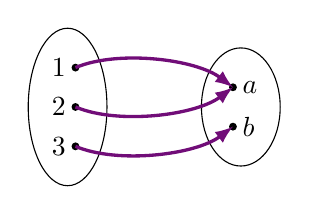
\begin{tikzpicture}
            \foreach \y in {-0.5, 0, 0.5} {
                \fill (0, \y) circle [radius = 0.05cm];
            }
            \foreach \y in {-0.25, 0.25} {
                \fill (2, \y) circle [radius = 0.05cm];
            }
            \node [left] at (0, -0.5) {\(3\)};
            \node [left] at (0, 0) {\(2\)};
            \node [left] at (0, 0.5) {\(1\)};
            \node [right] at (2, -0.25) {\(b\)};
            \node [right] at (2, 0.25) {\(a\)};
            \draw (-0.1, 0) circle [x radius = 0.5, y radius = 1];
            \draw (2.1, 0) circle [x radius = 0.5, y radius = 0.75];
            
            \draw [very thick, highlight, ->] (0, 0.5) to[bend left, looseness=0.75] (2, 0.25);
            \draw [very thick, highlight, ->] (0, 0) to[bend right, looseness=0.75] (2, 0.25);
            \draw [very thick, highlight, ->] (0, -0.5) to[bend right, looseness=0.75] (2, -0.25);
        \end{tikzpicture}
        \caption{A surjective function, \(g \colon \{1, 2, 3\} \to \{a, b\}\). Note that \(g(1) = g(2)\) but \(1 \ne 2\) and so the function fails to be injective.}
    \end{subfigure}
    \begin{subfigure}[t]{0.5\textwidth}
        \centering
        \tikzsetnextfilename{bijective-function}
        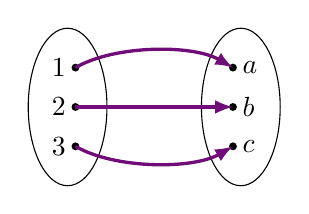
\begin{tikzpicture}
            \foreach \y in {-0.5, 0, 0.5} {
                \fill (0, \y) circle [radius = 0.05cm];
            }
            \foreach \y in {-0.5, 0, 0.5} {
                \fill (2, \y) circle [radius = 0.05cm];
            }
            \node [left] at (0, -0.5) {\(3\)};
            \node [left] at (0, 0) {\(2\)};
            \node [left] at (0, 0.5) {\(1\)};
            \node [right] at (2, 0.5) {\(a\)};
            \node [right] at (2, 0) {\(b\)};
            \node [right] at (2, -0.5) {\(c\)};
            \draw (-0.1, 0) circle [x radius = 0.5, y radius = 1];
            \draw (2.1, 0) circle [x radius = 0.5, y radius = 1];
            
            \draw [very thick, highlight, ->] (0, 0.5) to[bend left, looseness=0.75] (2, 0.5);
            \draw [very thick, highlight, ->] (0, 0) -- (2, 0);
            \draw [very thick, highlight, ->] (0, -0.5) to[bend right, looseness=0.75] (2, -0.5);
        \end{tikzpicture}
        \caption{A bijective function, \(h \colon \{1, 2, 3\} \to \{a, b, c\}\).}
    \end{subfigure}
    \caption{Injective, surjective, and bijective functions.}
\end{figure}

\begin{dfn}{Kernel}{}
    Given a map \(\varphi \colon A \to B\) the \defineindex{kernel} is defined as the set of elements of \(A\) which map to the trivial element of \(B\), which is the zero vector, \(\vv{0}\), if \(B\) is a vector space, or the identity if \(B\) is a group:
    \begin{equation}
        \ker\varphi \coloneqq \{a \in A \mid \varphi(a) \text{ is the trivial element of \(B\)}\} \subseteq A.
    \end{equation}
\end{dfn}

\begin{dfn}{Image}{}
    Given a map \(\varphi \colon A \to B\) the \defineindex{image} is set of \(b \in B\) for which there exists some \(a \in A\) such that \(\varphi(a) = b\):
    \begin{equation}
        \image\varphi = \varphi(A) \coloneqq \{b \in B \mid \exists \, a \in A \text{ such that } \varphi(a) = b\} \subseteq B.
    \end{equation}
\end{dfn}

\begin{dfn}{Empty Set}{}
    The \defineindex{empty set}, \(\emptyset\), is the set containing no elements.
\end{dfn}

\begin{dfn}{Kronecker Delta}{}
    The \defineindex{Kronecker delta}, \(\delta_{ij}\), is defined as
    \begin{equation}
        \delta_{ij} \coloneqq
        \begin{cases}
            1, & \text{if } i = j,\\
            0, & \text{if } i \ne j.
        \end{cases}
    \end{equation}
    Note that \(\delta_{ij}\) are the elements of the identity matrix.
\end{dfn}

\begin{dfn}{Levi-Civita Symbol}{}
    The \defineindex{Levi-Civita Symbol} in \(n\)-indices is the completely asymmetric (pseudo)tensor which is defined so that \(\varepsilon_{123\dotso n} \coloneqq 1\).
    Antisymmetry then means that \(\varepsilon_{1\dotsm i\dotsm j \dotsm n} = -\varepsilon_{1\dotsm j\dotsm i\dotsm n}\), for example \(\varepsilon_{213\dotsm n} = -1\).
    Antisymmetry also means that Levi--Civita symbol vanishes if it has repeated indices.
    
    Most commonly \(n = 3\) and
    \begin{equation}
        \varepsilon_{ijk} \coloneqq 
        \begin{cases}
            1, & \text{if } (i, j, k) = (1, 2, 3), (2, 3, 1), (3, 1, 2),\\
            -1, & \text{if } (i, j, k) = (1, 3, 2), (2, 1, 3), (3, 2, 1),\\
            0, & \text{if any index is repeated}.
        \end{cases}
    \end{equation}
\end{dfn}

\begin{dfn}{Equivalence Relations}{}
    Given two sets, \(A\) and \(B\), a \defineindex{relation}, \(R\), is a subset of \(A \times B \coloneqq \{(a, b) \mid a \in A \text{ and } b \in B\} \supseteq R\).
    We say that \(a \in A\) is related to \(b \in B\), which we denote with infix notation, \(a\mathbin{R}b\), if \((a, b) \in R\).
    
    If \(A = B\) in the above definition then we call \(R\) a \defineindex{binary!relation} on \(A\).
    
    A relation, \(\sim\), on a set \(A\) is a binary relation on \(A\) such that the following axioms hold for all \(a, b, c \in A\)
    \begin{itemize}
        \item \(\sim\) is \defineindex{reflexive}, so \(a \sim a\).
        \item \(\sim\) is \define{symmetric}\index{symmetric!relation}, so if \(a \sim b\) then \(b \sim a\).
        \item \(\sim\) is \defineindex{transitive}, so if \(a \sim b\) and \(b \sim c\) then \(a \sim c\).
    \end{itemize}
    
    An \defineindex{equivalence class} of an element \(a \in A\) under some equivalence relation, \(\sim\), is the set
    \begin{equation}
        [a] \coloneqq \{x \mid a \sim x\}.
    \end{equation}
    We call elements of \([a]\) representatives of the equivalence class.
    We denote the set of all equivalence classes by \(A/\sim\).
\end{dfn}

\begin{exm}{Equivalence Relations}{}
    \(=\) is the prototypical equivalence relation.
    
    Congruence modulo \(m \in \positiveintegers\) is an equivalence relation on \(\reals\).
    
    \(\sim\) defined by \(z\sim w\) if \(\abs{z} = \abs{w}\) is an equivalence relation on \(\complex\).
    
    \(\sim\) defined by \(\vv{v} \sim \vv{u}\) if \(\vv{u}\) and \(\vv{v}\) are parallel is an equivalence relation on \(\reals^n\).
\end{exm}

\begin{exm}{Isomorphism}{exm:isomorphism is equivalence relation}
    Isomorphisms, as defined in the text, are equivalence relations:
    \begin{itemize}
        \item Let \(A\) be a group, then the identity function, \(\mathrm{id}_A\colon A \to A\) defined by \(\mathrm{id}_A(a) = a\) for all \(a \in A\) is an isomorphism since \(\mathrm{id}_A(aa') = aa' = \mathrm{id}_A(a)\mathrm{id}_A(a')\) and clearly \(\mathrm{id}_A\) is invertible, and is its own inverse.
        \item Let \(A\) and \(B\) be isomorphic groups.
        Then there exists some bijection \(\varphi \colon A \to B\) such that \(\varphi(aa') = \varphi(a)\varphi(a')\).
        Since \(\varphi\) is a bijection \(\varphi^{-1}\colon B \to A\) exists and is also a bijection.
        Applying the inverse to both sides of the defining relation we have \(\varphi^{-1}(\varphi(aa')) = \varphi^{-1}(\varphi(a)\varphi(a'))\).
        Since \(\varphi\) is surjective any element of \(B\) can be written in the form \(b = \varphi(a)\) for some \(a \in A\) and so it follows that \(\varphi^{-1}(\varphi(aa')) = \varphi^{-1}(b)\varphi(b')\) where \(b, b' \in B\) are arbitrary, and we choose \(a, a' \in A\) to be such that \(b = \varphi(a)\) and \(b' = \varphi(a')\).
        From the defining relation for \(\varphi\) we know that \(\varphi(aa') = \varphi(a)\varphi(a') = bb'\).
        It follows that \(\varphi^{-1}(\varphi(aa')) = \varphi^{-1}(bb') = \varphi^{-1}(b)\varphi^{-1}(b')\), which means that \(B \isomorphic A\).
        \item Let \(A\), \(B\), and \(C\) be groups such that \(A \isomorphic B\) and \(B \isomorphic C\).
        Then there exists isomorphisms \(\varphi \colon A \to B\) and \(\psi\colon B \to C\).
        We claim that \(\psi\circ \varphi \colon A \to C\) is an isomorphism.
        Clearly \(\psi\circ \varphi\) is bijective, since \(\varphi^{-1}\circ \psi^{-1}\) is its inverse, as can be seen by considering \((\varphi^{-1}\circ \psi^{-1})((\psi\circ \varphi)(a)) = \varphi^{-1}(\psi^{-1}(\psi(\varphi(a)))) = \varphi^{-1}(\varphi(a)) = a\) for all \(a \in A\).
        
        It remains to show that \(\psi \circ \varphi\) is a homomorphism.
        To do so consider \((\psi \circ \varphi)(aa') = \psi(\varphi(aa')) = \psi(\varphi(a)\varphi(a'))\), which follows since \(\varphi\) is an isomorphism.
        Now write \(\varphi(a) = b\) and \(\varphi(a') = b'\), where \(b, b' \in B\).
        We then have \((\psi \circ \varphi)(aa') = \psi(bb') = \psi(b)\psi(b')\), which follows since \(\psi\) is an isomorphism.
        We then have \((\psi \circ \varphi)(aa') = \psi(b)\psi(b') = \psi(\varphi(b))\psi\varphi(b') = (\psi \circ \varphi)(b)(\psi \circ \varphi)(b')\), and so \(\psi\circ\varphi\) is a bijective homomorphism and hence an isomorphism, meaning \(A \isomorphic C\).
    \end{itemize}
\end{exm}

\section{Linear Algebra}
\subsection{Vectors}
\begin{dfn}{Vector Space}{}
    A vector space, \(V\), over a field, \(\field\), is a set of vectors, \(V\), with two operations, \(\cdot\colon \field \times V \to V\), known as scalar multiplication, and \(+\colon V\times V \to V\), known as vector addition, which are defined such that the following hold for all \(\vv{u}, \vv{v}, \vv{w} \in V\) and \(k, k' \in \field\):
    \begin{enumerate}
        \item \define{Associativity}\index{accociative}: \(\vv{u} + (\vv{v} + \vv{w}) = (\vv{u} + \vv{v}) + \vv{w}\),
        \item There exists a \define{zero vector}, \(\vv{0} \in V\), such that \(\vv{u} + \vv{0} = \vv{u}\).
        \item There exists \(-\vv{u} \in V\) such that \(\vv{u} + (-\vv{u}) = \vv{0}\).
        We write this as \(\vv{u} - \vv{u}\) for short.
        \item \define{Commutativity}\index{commutative}: \(\vv{u} + \vv{v} = \vv{v} + \vv{u}\).
        \item Distributivity of scalar multiplication over vector addition \(k(\vv{u} + \vv{v}) = k\vv{u} + k\vv{v}\).
        \item Distributivity of scalar multiplication over field addition \((k + k')\vv{u} = k\vv{u} + k'\vv{u}\).
        \item Compatibility of field and scalar multiplication \((kk')\vv{u} = k(k'\vv{u})\).
        \item \(1\vv{u} = \vv{u}\) where \(1\) is the multiplicative identity of \(\field\).
    \end{enumerate}
    Note that the first three axioms make \((V, +)\) a group and the fourth makes it Abelian.
\end{dfn}

\begin{dfn}{Hilbert Space}{def:hilbert space}
    A \defineindex{Hilbert space}, \(\hilbert\), is a vector space over either \(\reals\) or \(\complex\), equipped with an inner product that induces a complete metric.
    We shall assume a complex Hilbert space, for a real Hilbert space simply ignore any complex conjugates and replace \(\complex\) with \(\reals\).
    
    An \defineindex{inner product}\index{\(\innerprod{-}{-}\), inner product} is a function \(\innerprod{-}{-} \colon \hilbert \times \hilbert \to \complex\) such that for all \(\vv{u}, \vv{v}, \vv{w} \in \hilbert\) and \(k, k' \in \complex\)
    \begin{enumerate}
        \item \(\innerprod{-}{-}\) is linear in its second argument, that is
        \begin{equation}
            \innerprod{\vv{u}}{k\vv{v} + k'\vv{w}} = k\innerprod{\vv{u}}{\vv{v}} + k'\innerprod{\vv{u}}{\vv{w}}.
        \end{equation}
        \item \(\innerprod{-}{-}\) is conjugate symmetric:
        \begin{equation}
            \innerprod{\vv{u}}{\vv{v}} = \innerprod{\vv{v}}{\vv{u}}^*.
        \end{equation}
        \item \(\innerprod{-}{-}\) is positive definite, that is \(\innerprod{\vv{u}}{\vv{u}} \ge 0\) with equality only if \(\vv{u} = \vv{0}\).
    \end{enumerate}
    \begin{wrn}
        Mathematicians often define an inner product to be linear in its first argument, so
        \begin{equation}
            \innerprod{k\vv{u} + k'\vv{v}}{\vv{w}} = k\innerprod{\vv{u}}{\vv{w}} + k'\innerprod{\vv{v}}{\vv{w}}.
        \end{equation}
    \end{wrn}
    The first two axioms are sometimes combined to give an extra axiom that \(\innerprod{-}{-}\) is conjugate linear in its first argument (or second if we follow the other convention).
    That is
    \begin{equation}
        \innerprod{k\vv{u} + k'\vv{v}}{\vv{w}} = k^*\innerprod{\vv{u}}{\vv{w}} + k'^*\innerprod{\vv{v}}{\vv{w}}.
    \end{equation}
    We can then define a \defineindex{norm}\index{\(\norm{-}\), norm} on \(\hilbert\) by \(\norm{\vv{u}} \coloneqq \sqrt{\innerprod{\vv{u}}{\vv{u}}}\).
    
    The final condition for \(\hilbert\) to be a Hilbert space is completeness.
    Namely, that if the series \(\sum_{n=0}^{\infty} \vv{u_n}\) converges absolutely, so that \(\sum_{n=0}^{\infty} \norm{\vv{u_n}}\) converges to a finite value then the original series, \(\sum_{n=0}^{\infty} \vv{u_n}\), converges to some vector in \(\hilbert\).
\end{dfn}

\begin{exm}{}{}
    The set of \(n\)-tuples of complex numbers, \(\complex^n\), is a Hilbert space over \(\complex\) with the inner product
    \begin{equation}
        \innerprod{\vv{u}}{\vv{v}} = \innerprod{(u_1, \dotsc, u_n)}{(v_1, \dotsc, v_n)} \coloneqq \sum_{i=1}^n u_i^*v_i = u_i^*v_i
    \end{equation}
    where in the last term we use the Einstein summation convention.
\end{exm}

\begin{exm}{Functions}{}
    The space of square integrable functions on \(X \subseteq \reals^n\) forms a Hilbert space, denoted \(L^2(X)\).
    A function, \(f\colon X \to \complex\), is square integrable if\footnote{For this space to be complete (a requirement for Hilbert spaces) this must be a Lebesgue integral but in physics functions are usually nice enough that we can use the standard Riemann integral, which agrees with the Lebesgue integral when both exists.}
    \begin{equation}
        \int_{X} \abs{f(x)}^2 \dd{x}
    \end{equation}
    exists and is finite.
    For example, the function defined by \(f(x) = e^{-x^2}\) is an element of \(L^2(\reals)\).
    
    Given \(f, g \in L^2(X)\) we define the inner product in this space to be
    \begin{equation}
        \innerprod{f}{g} \coloneqq \int_{X} f^*(x)g(x) \dd{x}.
    \end{equation}
    \begin{rmk}
        Another subtly that arises here is that we actually need to consider elements of \(L^2(X)\) to be equivalence classes of functions which are equal almost everywhere (meaning that the measure of the set of points where they are not equal is zero).
        Otherwise, we may have some functions such that \(\innerprod{f}{g} = 0\) but \(f \ne g\) since \(f\) and \(g\) disagree on some set of points with a vanishing measure.
        We say that we are considering the functions mod the equivalence relation of being equal almost everywhere.
    \end{rmk}
    
    This is an important example since we can often identify \enquote{square integrable functions} with \enquote{possible wave functions}, since square-integrability is a requirement for us to be able to normalise a wave function, which we do so by the procedure
    \begin{equation}
        \psi \to \frac{\psi}{\norm{\psi}} = \frac{\psi}{\sqrt{\innerprod{\psi}{\psi}}} = \left( \int \abs{\psi(x)}^2 \dd{x} \right)^{-1/2} \psi.
    \end{equation}
    This only makes sense if \(\int \abs{\psi(x)}^2 \dd{x}\) is finite (and nonzero).
\end{exm}

\begin{ntn}{Bra-Ket Notation}{}
    In physics, particularly in quantum mechanics, we often use \defineindex{bra-ket notation}, developed by Dirac.
    We identify vectors, \(\vv{u}\), with \define{kets}\index{ket}\index{\(\ket{-}\), ket}, \(\ket{u}\), and dual vectors, \(\vv{v}\), with \define{bras}\index{bra}\index{\(\bra{-}\), bra}, \(\bra{v}\).
    The inner product \(\innerprod{\vv{u}}{\vv{v}}\) is then written \(\braket{v}{u}\)\index{\(\braket{-}{-}\), inner product}.
    This is the notation we will use for most of this course.
\end{ntn}

\begin{dfn}{Linear Operator}{}
    Given two vector spaces, \(V\) and \(W\), over some field, \(\field\), a function, \(f \colon V \to W\), is said to be a linear operator if for \(\vv{u}, \vv{v} \in V\) and \(k \in \field\) we have
    \begin{equation}
        f(\vv{u} + \vv{v}) = f(\vv{u}) + f(\vv{v}), \qqand f(k\vv{u}) = kf(\vv{u}).
    \end{equation}
    
    Instead of the function notation \(f(\vv{u})\) we typically use a multiplicative notation, \(A\vv{u}\), which is due to the fact that if \(V\) is finite dimensional then we can choose a basis and represent a linear map by a matrix.
    Using bra-ket notation also we have
    \begin{equation}
        A(\ket{u} + \ket{v}) = A\ket{u} + A\ket{v}, \qqand A(k\ket{u}) = kA\ket{u}.
    \end{equation}
    
    An operator is \defineindex{antilinear} if
    \begin{equation}
        A(\ket{u} + \ket{v}) = A\ket{u} + A\ket{v}, \qqand A(k\ket{u}) = k^*A\ket{u}.
    \end{equation}
    An example of such an operator is the time reversal operator, \(T\), which takes \(t \to -t\).
\end{dfn}

For simplicity from now on we will consider the complex vector space \(V = \complex^N\).
This is \(N\)-dimensional (\(\dim V = N\)), which we take to be finite, although many of these ideas work, possibly with slight modification, for infinite dimensional vector spaces.
Most of the time we will also consider linear operators from \(V\) to \(V\), since this is far more common in practice that linear operators from \(V\) to some different vector space, \(W\).

\begin{dfn}{Basis}{}
    Given a vector space, \(V\), we say that \(\{\ket{e_i}\}\) is a \defineindex{linearly independent} set if the only solution to
    \begin{equation}
        \lambda_i\ket{e_i} = \ket{0},
    \end{equation}
    where \(\ket{0}\) is the zero vector, is \(\lambda_i = 0\) for all \(i\).
    
    We say that \(\{\ket{e_i}\}\) is a \defineindex{basis} for \(V\) if \(\{\ket{e_i}\}\) is a linearly independent set and spans \(V\).
    That is given some \(\ket{u} \in V\) we can write
    \begin{equation}
        \ket{u} = u_i\ket{e_i}
    \end{equation}
    for some \(u_i \in \complex\).
    
    The number of vectors in a basis is the \defineindex{dimension} of the vector space, denoted \(\dim V\)\index{dim@\(\dim\), dimension}.
    
    We say that two vectors, \(\ket{u}, \ket{v} \in V\), are \define{orthogonal}\index{orthogonal!vectors} (with respect to some inner product) if \(\braket{u}{v} = 0\).
    
    We say that a vector, \(\ket{u} \in V\), is normalised if \(\norm{u} = \sqrt{\braket{u}{u}} = 1\).
    
    We say that \(\{\ket{e_i}\}\) is an orthonormal basis for \(V\) if it is a basis for \(V\), \(\ket{e_i}\) is normalised for all \(i\) and all of the basis vectors are mutually orthogonal.
    These last two conditions are summarised by requiring that
    \begin{equation}
        \braket{e_i}{e_j} = \delta_{ij}.
    \end{equation}
\end{dfn}

\begin{dfn}{Completeness Relation}{}
    Given a vector space, \(V\), and an orthonormal basis, \(\{\ket{e_i}\}\), we can write the identity operator, \(\ident\), as
    \begin{equation}
        \ident = \sum_{i=1}^{N} \ket{e_i}\bra{e_i}.
    \end{equation}
    Recall that the identity operator is defined such that\index{\(\ident\), identity matrix}
    \begin{equation}
        \ident\ket{u} = \ket{u}
    \end{equation}
    for all \(\ket{u} \in V\).
\end{dfn}

\begin{dfn}{Partition of the Identity}{}
    A \defineindex{projection operator}, \(P_i\), is an operator satisfying
    \begin{equation}
        P_iP_j = \delta_{ij}P_i, \qqand P_i^\hermit = P_i.
    \end{equation}
    A \defineindex{partition of the identity} is a collection of projection operators, \(\{P_j\}\), such that
    \begin{equation}
        \ident = \sum_{j=1}^{N_P} P_j
    \end{equation}
    where \(N_P = \abs{\{P_j\}}\) is the number of projection operators in the partition.
    We can write each partition operator as
    \begin{equation}
        P_j = \sum_{i=1}^{N_j} \ket{e_i}\bra{e_i}
    \end{equation}
    where \(N_j\) are such that
    \begin{equation}
        \dim V = N = \sum_{j=1}^{N_P}N_j.
    \end{equation}
\end{dfn}

\begin{dfn}{Matrix Element}{}
    Given a linear operator, \(A \colon V \to V\), and an orthonormal basis, \(\{\ket{e_i}\}\), we define the \define{matrix elements}\index{matrix element} to be
    \begin{equation}
        A_{ij} \coloneqq \braket{e_i}{Ae_j} = \bra{e_i}A\ket{e_j}
    \end{equation}
    where \(A\) is understood to act on the right and \(\ket{Ae_j} \coloneqq A\ket{e_j}\).
    
    If we know the matrix elements of \(A\) we can reconstruct \(A\) using
    \begin{equation}
        A = \sum_{i=1}^{N}\sum_{j=1}^{N} A_{ij}\ket{e_i}\bra{e_j}.
    \end{equation}
\end{dfn}

\begin{dfn}{Eigenvalues and Eigenvectors}{}
    Given a linear operator \(A\), we call \(\ket{v_i}\) an \defineindex{eigenvector} and \(\lambda_i\in\complex\) an \defineindex{eigenvalue} if
    \begin{equation}
        A\ket{v_i} = \lambda_i\ket{v_i}.
    \end{equation}
    There are \(N\) solutions to this, which follows from the \defineindex{characteristic polynomial}, \(\det(A - \lambda\ident) = 0\), having \(N\) solutions, which in turn follows from the fundamental theorem of algebra.
\end{dfn}

\subsection{Matrices}
\begin{dfn}{Transpose and Hermitian Conjugate}{}
    Given a matrix, \(A\), with matrix elements \(A_{ij}\), the \defineindex{transpose}\index{\(-^\trans\), transpose} matrix, \(A^\trans\), has matrix elements \(A^\trans_{ij} = A_{ji}\).
    
    A matrix is \defineindex{symmetric} if \(A^\trans = A\), or \defineindex{antisymmetric} if \(A^\trans = -A\).
    
    Given a matrix, \(A\), with matrix elements \(A_{ij}\), the \define{Hermitian conjugate}\index{Hermitian!conjugate}\index{\(-^\hermit\), Hermitian conjugate}, \(A^\hermit\), has matrix elements \(A^\hermit_{ij} = A_{ji}^*\).
    Here \(^*\) denotes the \define{complex conjugate}\index{complex!conjugate}\index{\(-^*\), complex conjugate}, so \((x + iy)^* = x - iy\) and \((r\e^{i\vartheta})^* = r\e^{-\vartheta}\) for \(x, y, r, \vartheta \in \reals\).
    That is the Hermitian conjugate is the complex conjugate of the transpose.
    
    A matrix is \defineindex{Hermitian} if \(A^\hermit = A\), or \defineindex{anti-Hermitian} if \(A^\hermit = -A\).
\end{dfn}

\begin{lma}{}{}
    The eigenvalues of a Hermitian matrix are real.
    \begin{proof}
        Let \(A\) be a Hermitian matrix and \(\vv{v}\) an eigenvector with nonzero eigenvalue \(\lambda\).
        Note that this means \(\vv{v}\) is nonzero.
        If \(0\) is an eigenvalue of \(A\) then this is real, so we need not consider this case further.
        By definition \(A\vv{v} = \lambda\vv{v}\).
        Taking the Hermitian conjugate of both sides we get \(\vv{v}^\hermit A^\hermit = \lambda^*\vv{v}^\hermit\), where we have used \((XY)^\hermit = Y^\hermit X^\hermit\).
        Multiplying both sides on the right by \(\vv{v}\) we get \(\vv{v}^\hermit A \vv{v} = \lambda^*\vv{v}^\hermit \vv{v}\).
        Identifying \(A\vv{v} = \lambda\vv{v}\) on the left-hand side this becomes \(\vv{v}^\hermit \lambda \vv{v} = \lambda\vv{v}^\hermit \vv{v} = \lambda^*\vv{v}^\hermit \vv{v}\).
        It follows that we must have \(\lambda = \lambda^*\), which means we must have \(\lambda \in \reals\).
    \end{proof}
\end{lma}

We can choose the eigenvalues of a Hermitian matrix to be orthonormal, and hence they form a basis for the vector space.
In this basis the matrix will be diagonal and the values on the diagonal are simply the eigenvalues.

Given a Hermitian matrix, \(A\), with eigenvalues \(\lambda_i\) and corresponding eigenvectors \(\ket{v_i}\) we can write this matrix as
\begin{equation}
    A = \sum_{i=1}^{N} \lambda_i\ket{v_i}\bra{v_i}.
\end{equation}
This is diagonalised by the transformation \(V^\hermit A V\) where
\begin{equation}
    V = \sum_{i=1}^{N} \ket{v_i}\bra{e_i}
\end{equation}
where \(\ket{e_i}\) are the basis vectors in the original basis.
It is easy to see that this transform gives the desired result:
\begin{align}
    V^\hermit AV &= \underbrace{\ket{e_i}\bra{v_i}}_{=V^\hermit}  \underbrace{(\lambda_j \ket{v_j}\bra{v_j})}_{=A}\underbrace{\ket{v_k}\bra{e_k}}_{=V}\\
    &= \lambda_j \ket{e_i}\braket{v_i}{v_j}\braket{v_j}{v_k}\bra{e_k}\\
    &= \lambda_j \delta_{ij}\delta_{jk} \ket{e_i}\bra{e_k}\\
    &= \lambda_i \ket{e_i}\bra{e_i}
\end{align}
This last term is just a diagonal matrix with the eigenvalues, \(\lambda_i\), as the diagonal elements, which is exactly what we wanted.

For non-Hermitian matrices it is possible that the eigenvalues aren't linearly independent.
In this case the best we can do is Jordan normal form where the eigenvalues are on the diagonal and all other entries are either zero or one for elements in the subspace of degenerate eigenvalues.

\begin{dfn}{Inverse}{}
    The \defineindex{inverse}\index{\(-^{-1}\), inverse} of a matrix, \(A\), is the matrix \(A^{-1}\) such that \(A^{-1}A = AA^{-1} = \ident\).
    Such a matrix exists only if the determinant is non-zero.
\end{dfn}

An equivalent requirement for \(A^{-1}\) to exist is for \(A\) to have no zero eigenvalues.
For a Hermitian matrix the inverse in the eigenbasis is simply
\begin{equation}
    A^{-1} = \diag(1/\lambda_1, \dotsc, 1/\lambda_N).
\end{equation}

\begin{dfn}{Orthogonal and Unitary}{}
    A matrix, \(O\), is \define{orthogonal}\index{orthogonal!matrix} if \(O^\trans O = \ident\), that is \(O^\trans = O^{-1}\).
    
    A matrix, \(U\), is \defineindex{unitary} if \(U^\hermit U = \ident\), that is \(U^\hermit = U^{-1}\).
\end{dfn}

The following holds:
\begin{equation}
    \braket{u}{Av} = \bra{u}A\ket{v} = \braket{A^\hermit u}{v}.
\end{equation}
For a unitary matrix, \(U\), this implies
\begin{equation}
    \braket{Uu}{Uv} = \bra{u}U^\hermit U\ket{v} = \bra{u}\ident \ket{v} = \braket{u}{v}.
\end{equation}
We say that unitary transforms preserve the inner product, or that the inner product is invariant under unitary transforms.

\begin{dfn}{Trace}{}
    The \defineindex{trace}\index{tr@\(\tr\), trace} of a matrix, \(A\) is
    \begin{equation}
        \tr A \coloneqq \sum_{i} \bra{e_i} A_i \ket{i} = A_{ii}
    \end{equation}
    where in the last term we are using the Einstein summation convention to sum over \(i\).
\end{dfn}

The trace of a matrix is simply the sum of its eigenvalues, this doesn't just hold for Hermitian matrices.

The trace is cyclic, meaning \(\tr(AB) = \tr(BA)\), \(\tr(ABC) = \tr(BCA) = \tr(CAB)\), etc.

The trace is linear, meaning \(\tr(k A) = k\tr(A)\) for scalar \(k\).

\(\innerprod{A}{B} \coloneqq \tr(A^\hermit B)\) is an inner product on the vector space of matrices.
This is called the \defineindex{Gram--Schmidt inner product}.

\begin{dfn}{Determinant}{}
    The \defineindex{determinant}\index{det@\(\det\), determinant}\index{\(\abs{-}\), determinant} of a matrix, \(A\), is 
    \begin{equation}
        \det A = \abs{A} = \coloneqq \varepsilon_{i_1\dotso i_N} A_{1i_1}\dotsm A_{Ni_N}
    \end{equation}
    with summation over indices implied.
\end{dfn}

The determinant of a matrix is the product of its eigenvalues.

The determinant of a product is the product of the determinants:
\begin{equation}
    \det(AB) = \det(A)\det(B) = \det(B)\det(A) = \det(BA).
\end{equation}

\begin{dfn}{Diagonal}{}
    A matrix, \(A\), is \defineindex{diagonal} if \(A_{ij} = 0\) for \(i \ne j\).
    
    A matrix, \(A\), is \defineindex{block diagonal} if it can be written in the form
    \begin{equation}
        A = 
        \begin{pmatrix}
            A_1 & 0 & 0 & \dots & 0\\
            0 & A_2 & 0 & \dots & 0\\
            \vdots & \vdots & \vdots & \ddots & \vdots\\
            0 & 0 & 0 & 0 & A_n
        \end{pmatrix}
    \end{equation}
    where \(A_i\) are square matrices and the \(0\)s represent matrices where all elements are zero.
\end{dfn}    

\subsection{Combining Vector Spaces}
\begin{dfn}{Direct Sum}{dfn:direct sum}
    Given vector spaces \(V\) and \(W\) we call \(V\directsum W\)\index{\(\directsum\), direct sum} the \define{direct sum}\index{direct!sum}.
    It is defined by associating with each pair of vectors, \(\ket{v_i} \in V\) and \(\ket{w_a} \in W\), a vector \(\ket{v_i} \directsum \ket{w_i} = \ket{v_i \directsum w_a} \in V \directsum W\) and extending the inner product to
    \begin{equation}
        \braket{v_i \directsum w_a}{v_j \directsum w_b}_{V\directsum W} \coloneqq \braket{v_i}{v_j}_{V} + \braket{w_a}{w_b}_{W}
    \end{equation}
    where the subscripts denote which vector space the inner product is in.
    Note that the notation \(\ket{v \directsum w}\) is non-standard.
    
    The dimension of \(V \directsum W\) is
    \begin{equation}
        \dim(V \directsum W) = \dim V + \dim W.
    \end{equation}
    
    Given \(A \in \generalLinear(V)\) and \(B \in \generalLinear(W)\) the direct sum, \(A \directsum B\), acts on \(\ket{v} \directsum \ket{w} \in V \directsum W\) as
    \begin{equation}
        (A \directsum B)(\ket{v} \directsum \ket{w}) \coloneqq (A\ket{v}) \directsum (B\ket{w}).
    \end{equation}
    This shows we can think of \(V \directsum W\) as a \((\dim V + \dim W)\)-dimensional vector space with operators represented by \((v + w) \times (v + w)\) block diagonal matrices:
    \begin{equation}
        A \directsum B = 
        \begin{pmatrix}
            A & 0\\
            0 & B
        \end{pmatrix}
        .
    \end{equation}
    We then think of \(\ket{v} \directsum \ket{w} \in V \directsum W\) as \((v_1, \dotsc, v_{\dim V}, w_1, \dotsc, w_{\dim W})\).
\end{dfn}

An important question is can a given vector space be written as a direct sum of vector spaces, this occurs when considering the irreducibility of representations.

\begin{dfn}{Direct Product}{}
    Given vector spaces \(V\) and \(W\) we call \(V \directproduct W\)\index{\(\directproduct\), direct product} the \define{direct product}\index{direct!product}.
    It is defined by associating with each pair of vectors, \(\ket{v_i} \in V\) and \(\ket{w_a} \in W\), a vector \(\ket{v_i} \directproduct \ket{w_a} = \ket{v_i \directproduct w_a} \in V \directproduct W\) and extending the inner product to
    \begin{equation}
        \braket{v_i \directproduct w_a}{v_j \directproduct w_b}_{V\directproduct W} \coloneqq \braket{v_i}{v_j}_{V}\braket{w_a}{w_b}
    \end{equation}
    where the subscripts denote which vector space the inner product is in.
    Note that the notation \(\ket{v\directproduct w}\) is non-standard.
    
    The dimension of \(V\directproduct W\) is
    \begin{equation}
        \dim(V\directproduct W) = \dim(V) \dim(W).
    \end{equation}
    
    Given \(A \in \generalLinear(V)\) and \(B \in \generalLinear(W)\) the direct product, \(A \directproduct B\), acts on \(\ket{v}\directproduct \ket{w} \in V\directproduct W\) as
    \begin{equation}
        (A\directproduct B)(\ket{v}\directproduct \ket{w}) = (A\ket{v})\directproduct(B\ket{w}).
    \end{equation}
\end{dfn}

\begin{app}{}{}
    In quantum mechanics we can combine states from different Hilbert spaces representing different properties with direct products.
    For example, given an electron wave function with a spatial component and a spin component the direct product of these gives the state of the electron.
\end{app}

The direct product plays a role in representation theory in terms of what we will call Kronecker products.
These can be used to obtain all representations from the fundamental representations.
        \chapter{Groups}
\section{Finite Groups}

\begin{dfn}{}{}
    The \defineindex{trivial group} is the group containing only the identity, \(\{e\}\).
    It is the only group of order 1.
    
    
    \begin{multicols}{2}
        \begin{itemize}
            \item Order 1.
            \item Rank 1.
            \item Cyclic.
            \item Abelian.
        \end{itemize}
    \end{multicols}
    The trivial group is isomorphic to \(\integers_1\), \(S_1\), and \(\specialOrthogonal(1)\).
\end{dfn}

\begin{dfn}{}{}
    \(\integers_2\) is the cyclic group of order 2, see \cref{dfn:cyclic group}.
    It is the only group of order 2.
    
    
    \begin{multicols}{2}
        \begin{itemize}
            \item Order 2.
            \item Rank 1.
            \item Cyclic.
            \item Abelian.
        \end{itemize}
    \end{multicols}
    \(\integers_2\) is isomorphic to \(S_2\).
\end{dfn}

\begin{dfn}{}{}
    \(\integers_3\) is the cyclic group of order 3, see \cref{dfn:cyclic group}.
    It is the only group of order 3.
    
    \begin{multicols}{2}
        \begin{itemize}
            \item Order 3.
            \item Rank 1.
            \item Cyclic.
            \item Abelian.
        \end{itemize}
    \end{multicols}
\end{dfn}

\begin{dfn}{}{}
    \(\integers_4\) is the cyclic group of order 4, see \cref{dfn:cyclic group}.
    It is one of two groups of order 4.
    
    \begin{multicols}{2}
        \begin{itemize}
            \item  Order 4.
            \item Rank 1.
            \item Cyclic.
            \item Abelian.
        \end{itemize}
    \end{multicols}
\end{dfn}

\begin{dfn}{}{}
    \(\integers_2\times\integers_2\) is the \defineindex{Klein \textit{Vierergruppe}}.
    It is one of two groups of order 4.
    It is a direct product of two copies of \(\integers_2\).
    
    \begin{multicols}{2}
        \begin{itemize}
            \item Order 4.
            \item Rank 2.
            \item Abelian.
        \end{itemize}
    \end{multicols}
\end{dfn}

\begin{dfn}{}{}
    \(S_3\) is the permutation group on 3 elements, see \cref{dfn:permutation group}.
    
    \begin{multicols}{2}
        \begin{itemize}
            \item Order 6.
            \item Rank 2.
            \item Non-Abelian.
        \end{itemize}
    \end{multicols}
\end{dfn}

\begin{dfn}{}{}
    The \defineindex{quaternion group}, \(Q\)\index{Q@\(Q\), quaternion group}, has the group presentation
    \begin{equation}
        Q = \presentation{-e, i, j, k}{(-e)^2 = e, i^2 = j^2 = k^2 = ijk = e}.
    \end{equation}
    
    \begin{multicols}{2}
        \begin{itemize}
            \item Order 8.
            \item Rank 2.
            \item Non-Abelian.
        \end{itemize}
    \end{multicols}
    The Pauli matrices provide a two-dimensional complex representation by the correspondence \((-e, i, j, k) \to (-\ident, \sigma_1, \sigma_2, \sigma_3)\).
\end{dfn}

\subsection{Other Finite Groups}
\begin{dfn}{}{dfn:cyclic group}
    The \defineindex{cyclic group} of order \(n\), denoted \(\integers_n\), is given by the presentation
    \begin{equation}
        \integers_n = \presentation{a}{a^n = e}.
    \end{equation}
    Identifying \(a = \e^{2i\pi/n}\) and the operation as multiplication we get a group formed from the \(n\)th roots of unity.
    Identifying \(a = 1\) and the operation as addition modulo \(n\) we get a group formed from \(\{0, \dotsc, n-1\}\).
    
    \begin{multicols}{2}
        \begin{itemize}
            \item Order \(n\).
            \item Rank 1.
            \item Cyclic.
            \item Abelian.
        \end{itemize}
    \end{multicols}
    All finite cyclic groups are isomorphic to \(\integers_n\) for some \(n\).
\end{dfn}

\begin{dfn}{}{dfn:permutation group}
    The \defineindex{permutation group} on \(n\) objects is the group of all permutations (bijections) of \(\{1, \dotsc, n\}\), with function composition as the group operation.
    
    \begin{multicols}{2}
        \begin{itemize}
            \item Order \(n!\).
            \item Rank 2.
            \item Non-Abelian (\(n > 2\)).
        \end{itemize}
    \end{multicols}
    \(S_1\) and \(S_0\) are isomorphic to the trivial group.
    
    \(S_2\) is isomorphic to \(\integers_2\).
\end{dfn}

\section{Discrete Groups}

\begin{dfn}{}{}
    The integers, \(\integers\), under addition.
    
    \begin{multicols}{2}
        \begin{itemize}
            \item Rank 1.
            \item Cyclic.
            \item Abelian.
        \end{itemize}
    \end{multicols}
\end{dfn}

\begin{dfn}{}{}
    The rational numbers, \(\rationals\), under addition.
    
    \begin{multicols}{2}
        \begin{itemize}
            \item Abelian.
        \end{itemize}
    \end{multicols}
\end{dfn}

\begin{dfn}{}{}
    The nonzero rational numbers, \(\rationals^*\), under multiplication.
    
    \begin{multicols}{2}
        \begin{itemize}
            \item Abelian.
        \end{itemize}
    \end{multicols}
\end{dfn}

\section{Continuous Groups}

\subsection{Scalars}

\begin{dfn}{}{}
    The real numbers, \(\reals\), under addition.
    
    \begin{multicols}{2}
        \begin{itemize}
            \item Abelian.
        \end{itemize}
    \end{multicols}
    \((\reals, +)\) is isomorphic to \((\reals_{>0}, \cdot)\).
\end{dfn}

\begin{dfn}{}{}
    The nonzero real numbers, \(\reals^*\), under multiplication.
    
    \begin{multicols}{2}
        \begin{itemize}
            \item Abelian.
        \end{itemize}
    \end{multicols}
\end{dfn}
    
\begin{dfn}{}{}
    The complex numbers, \(\complex\), under addition.
    
    \begin{multicols}{2}
        \begin{itemize}
            \item Abelian.
        \end{itemize}
    \end{multicols}
\end{dfn}

\begin{dfn}{}{}
    The nonzero complex numbers, \(\complex^*\), under multiplication.
    
    \begin{multicols}{2}
        \begin{itemize}
            \item Abelian.
        \end{itemize}
    \end{multicols}
\end{dfn}
    
\subsection{Matrices}

\begin{dfn}{}{}
    The \defineindex{general linear group}\index{GL(n, F)@\(\generalLinear(n, \field)\), general linear group}
    \begin{equation}
        \generalLinear(n, \field) = \left\{ M \in \matrices{n}{\field} \mid \det M \ne 0 \right\}.
    \end{equation}
    If \(V\) is a vector space of dimension \(n\) over \(\field\) then this group is also denoted \(\generalLinear(V)\).
    If \(\field\) is obvious from context then this group is denoted \(\generalLinear(n)\).
    
    \begin{multicols}{2}
        \begin{itemize}
            \item Non-Abelian (\(n > 1\)).
        \end{itemize}
    \end{multicols}
\end{dfn}

\begin{dfn}{}{}
    The \defineindex{special linear group}\index{SL(n, F)@\(\specialLinear(n, \field)\), special linear group}
    \begin{equation}
        \specialLinear(n, \field) = \{ M \in \matrices{n}{\field} \mid \det M = 1 \}.
    \end{equation}
    If \(V\) is a vector space of dimension \(n\) over \(\field\) then this group is also denoted \(\specialLinear(V)\).
    If \(\field\) is obvious from context then this group is denoted \(\specialLinear(n)\).
    
    \begin{multicols}{2}
        \begin{itemize}
            \item Non-Abelian (\(n > 1\)).
        \end{itemize}
    \end{multicols}
    
    \(\specialLinear(n, \field)\) is a subgroup of \(\generalLinear(n, \field)\).
\end{dfn}

\begin{dfn}{}{}
    The \defineindex{orthogonal group}\index{O(n)@\(\orthogonal(n)\), orthogonal group}
    \begin{equation}
        \orthogonal(n) = \{ O \in \matrices{n}{\reals} \mid O^\trans O = OO^\trans = \ident \}.
    \end{equation}
    
    \begin{multicols}{2}
        \begin{itemize}
            \item Non-Abelian (\(n > 1\)).
        \end{itemize}
    \end{multicols}

    \(\orthogonal(n)\) is a subgroup of \(\generalLinear(n, \reals)\).
    
    \(\orthogonal(n)\) is the group of distance preserving transformations of Euclidean space which leave the origin invariant.
    
    \(\orthogonal(n)\) is the group of rotations and inversions of \(\reals^n\).
\end{dfn}

\begin{dfn}{}{}
    The \defineindex{special orthogonal group}\index{SO(n)@\(\specialOrthogonal(n)\), special orthogonal group}
    \begin{equation}
        \specialOrthogonal(n) = \{ O \in \matrices{n}{\reals} \mid O^\trans O = OO^\trans = \ident \text{ and } \det O = 1 \}.
    \end{equation}
    
    \begin{multicols}{2}
        \begin{itemize}
            \item Non-Abelian (\(n > 1\)).
        \end{itemize}
    \end{multicols}
    
    \(\specialOrthogonal(n)\) is a subgroup of \(\orthogonal(n)\) and \(\specialLinear(n, \reals)\).
    
    \(\specialOrthogonal(n)\) is the group of rotations of \(\reals^n\).
    
    \(\specialOrthogonal(2)\) is isomorphic to \(\unitary(1)\) and the circle group, \(\mathbb{T} = \{z \in \complex \mid \abs{z} = 1\}\) under multiplication.
\end{dfn}

\begin{dfn}{}{}
    The \defineindex{unitary group}\index{U(n)@\(\unitary(n)\), unitary group}
    \begin{equation}
        \unitary(n) = \{ U \in \matrices{n}{\complex} \mid U^\hermit U = UU^\hermit = \ident \}.
    \end{equation}
    
    \begin{multicols}{2}
        \begin{itemize}
            \item Non-Abelian (\(n > 1\)).
        \end{itemize}
    \end{multicols}
    
    \(\unitary(n)\) is a subgroup of \(\generalLinear(n, \complex)\).
    
    \(\unitary(n)\) is the group which preserves the standard inner product on \(\complex^n\).
    
    \(\unitary(1)\) is isomorphic to \(\specialOrthogonal(2)\) and the circle group, \(\mathbb{T} = \{z \in \complex \mid \abs{z} = 1\}\) under multiplication.
\end{dfn}

\begin{dfn}{}{}
    The \defineindex{special unitary group}\index{SU(n)@\(\specialUnitary(n)\), special unitary group}
    \begin{equation}
        \specialUnitary(n) = \{ U \in \matrices{n}{\complex} \mid U^\hermit U = UU^\hermit = \ident \text{ and } \det U = \ident \}.
    \end{equation}
    
    \begin{multicols}{2}
        \begin{itemize}
            \item Non-Abelian (\(n > 1\)).
        \end{itemize}
    \end{multicols}

    \(\specialUnitary(n)\) is a subgroup of \(\unitary(n)\) and \(\specialLinear(n, \complex)\).
\end{dfn}

\begin{dfn}{}{}
    The \defineindex{isometries of Euclidean space}
    \begin{equation}
        \ISO(n) = \orthogonal(n) \ltimes \reals^n
    \end{equation}
    where \((R, \vv{a}) (R', \vv{a'}) \coloneqq (RR', \vv{a} + R\vv{a'})\).
    \begin{multicols}{2}
        \begin{itemize}
            \item Non-Abelian
        \end{itemize}
    \end{multicols}
    \(\ISO(n)\) is the group of distance preserving transformations of Euclidean space.
    
    \(\ISO(n)\) is the group of rotations, reflections, and translations of \(\reals^n\).
    
    \(\ISO(n)\) has both \(\orthogonal\) and \(\reals^n\) as normal subgroups.
\end{dfn}

\begin{dfn}{}{}
    The \defineindex{Lorentz group}, \(\orthogonal(1, 3)\)\index{O(1, 3)@\(\orthogonal(1, 3)\), Lorentz group}, is the group of all Lorentz transformations of Minkowski space.
    \begin{multicols}{2}
        \begin{itemize}
            \item Non-Abelian.
        \end{itemize}
    \end{multicols}

    \(\orthogonal(1, 3)\) is the group that preserves the quadratic form \((t, x, y, z) \mapsto t^2 - x^2 - y^2 - z^2\).
    
    \(\specialOrthogonal^+(1, 3)\) is the subgroup of \(\orthogonal(1, 3)\) which preserves the orientation of space (S for special, that is unit determinant) and direction of time (that's what the \(+\) represents).
\end{dfn}

\begin{dfn}{}{}
    The \defineindex{Poincar\'e group} is the group of all isometries of Minkowski space, sometimes denoted \(\isometry(1, 3)\)\index{ISO(1, 3)@\(\isometry(1, 3)\), Poincar\'e group}.
    That is it is the group of all Lorentz transformations and translations.
    \begin{multicols}{2}
        \begin{itemize}
            \item Non-Abelian.
        \end{itemize}
    \end{multicols}
    
    The Poincar\'e group can be identified as the semidirect product \(\isometry(1, 3) = \reals^{1,3} \rtimes  \orthogonal(1, 3)\) where \(\reals^{1,3}\) is the group of spacetime translations of Minkowski space and \(\orthogonal(1, 3)\) is the Lorentz group.
\end{dfn}

        \chapter{Manifolds}\label{app:manifold}
\begin{rmk}
    The notes in this section are repeated from the notes for general relativity so for more details look at those notes.
\end{rmk}
The theory of Lie groups starts by defining them as manifolds with a group structure, or groups with a manifold structure.
In order to make this rigorous we need to define a manifold.
We will define a real manifold for simplicity and the definition of a complex manifold is nearly identical replacing \(\reals\) with \(\complex\) and requiring maps be holomorphic instead of smooth.

I go into far more detail here than necessary.
I also make statements like \enquote{\(\category{Top}\) is the category of topological spaces with continuous functions as morphisms and homeomorphisms as isomorphisms} without explanation, these sorts of statement aren't important if you don't understand them.

\section{Manifolds}
We start with a rough definition of a manifold which lacks a few details which we will fill out later.
For our purposes this rough definition is sufficient and the full definition is for completeness.
\begin{dfn}{Manifold}{}
    A \defineindex{manifold} is a space where we can locally introduce Cartesian coordinates such that different choices of local coordinates will give compatible descriptions and by defining sets of local coordinates covering the whole space we have complete information about the space.
\end{dfn}

A manifold is parametrised continuously and differentiably as an \(n\)-tuple of real numbers, \((x^1, \dotsc, x^n) \in \reals^n\), which are the coordinates of the point.
We can connect two points with a curve parametrised by some \(\lambda \in \reals\) such that derivatives of the coordinates along this path exist, that is \(\diff{x^i}/{\lambda}\) exists for all \(i = 1, \dotsc, n\).

By this definition it should be clear that Euclidean space, where non-relativistic mechanics takes place, is a manifold.
However, not all manifolds are as nice as Euclidean space, for example Euclidean space has a metric (way to measure distance), which not all manifolds do.
Locally all manifolds behave like a subset of Euclidean space due to their differentiable nature.

\subsection{Topology}
\begin{dfn}{Topological Space}{}
    A \define{topological space}\index{topological!space}, \((X, \mathcal{T})\), is a set, \(X\), and a collection of subsets of \(X\), \(\mathcal{T} \subset \mathcal{P}(X)\), called the \defineindex{topology}, such that
    \begin{itemize}
        \item \(X \in \mathcal{T}\),
        \item \(\emptysetAlt \in \mathcal{T}\),
        \item \(\mathcal{T}\) is closed under unions, that is if \(\{U_i\}_{i \in I} \subseteq \mathcal{T}\) then\vspace{-1ex}
        \begin{equation}
            \bigcup_{i\in I} U_i \in \mathcal{T},
        \end{equation}\vspace{-4ex}
        \item \(\mathcal{T}\) is closed under finite intersections, that is if \(\{U_i, \dotsc, U_N\} \subseteq \mathcal{T}\) then\vspace{-4ex}
        \begin{equation}
            \bigcap_{i = 1}^{N} U_i \in \mathcal{T}.
        \end{equation}
    \end{itemize}\vspace{-1ex}
    We call the elements of \(\mathcal{T}\) \define{open sets}\index{open set}.
\end{dfn}

It is common to refer to \(X\) as a topological space and then specify \(\mathcal{T}\) separately, or just leave \(\mathcal{T}\) implicit, much in the same way that we might define a group \(G\) and operation \(\cdot\), when more formally it might be more correct to call \((G, \cdot)\) and \(G\) the underlying set.

Topological spaces can be quite abstract, for example the following topology makes \((\{a, b, c, d\}, \mathcal{T})\) a topological space:
\begin{equation}
    \mathcal{T} = \{\emptysetAlt, \{a, b, c, d\}, \{a, b\}, \{c, d\}\}.
\end{equation}
We only deal with more familiar topological spaces.
We can define different topologies using a basis.

\begin{dfn}{Topological Basis}{}
    A \define{basis}\index{topological!basis} for a topology on some set \(X\) is a collection of sets, \(\mathcal{B} \subseteq \mathcal{P}(X)\) such that
    \begin{itemize}
        \item the elements of \(\mathcal{B}\) cover \(X\), that is for all \(x \in X\) there exists some \(B \in \mathcal{B}\) such that \(x \in B\).
        \item given \(B_1, B_2 \in \mathcal{B}\) for all \(x \in B_1 \cap B_2\) there exists some \(B_3 \in \mathcal{B}\) such that \(x \in B_3\) and \(B_3 \subseteq B_1 \cap B_2\).
    \end{itemize}
    The topology generated by a basis, \(\mathcal{B}\), is then defined to be the set of all subsets \(U \subseteq X\) such that\vspace{-0.5ex}
    \begin{equation}
        U = \bigcup_{B_i \in B \subseteq \mathcal{B}} B_i.
    \end{equation}\vspace{-0.5ex}
    That is all elements of the topology are unions of basis sets.
\end{dfn}

Using this definition we can define the \defineindex{standard topology} on \(\reals^n\) as the topology generated by the basis of open balls in \(\reals^n\), where by an open ball we mean
\begin{equation}
    B = \{\vv{r} \in \reals^n \mid \abs{\vv{r} - \vv{a}} \le 1 \text{ for some } \vv{a} \in \reals^n\}
\end{equation}
with \(\abs{\vv{r}} = \sum_i x_i^2\) being the usual Euclidean metric.
This is not the only topology on \(\reals^n\) but it is the only one we care about.

Let \(X\) and \(Y\) be topological spaces with topologies \(\mathcal{T}_X\) and \(\mathcal{T}_Y\) respectively.
Then we can define a function, \(f \colon X \to Y\).
The \defineindex{preimage} of some \(S \subseteq Y\) under this function is the set
\begin{equation}
    f^*(S) = f^{-1}(S) \coloneqq \{a \in X \mid f(a) \in S\} \subseteq X.
\end{equation}
The notation \(f^{-1}\) suggests that this is related to the inverse of the function \(f\), and indeed if the inverse exists then it is, as the preimage is the image of the inverse restricted to \(S\).

The function \(f \colon X \to Y\) is \defineindex{continuous} if all preimages of open sets of \(Y\) are open sets of \(X\), that is if \(f^*(U_Y) \in \mathcal{T}_X\) for all \(U_Y \in \mathcal{T}_Y\).
With the standard topology for \(\reals^n\) this definition coincides with the normal \(\varepsilon\)-\(\delta\) definition of continuity from analysis.

An invertible (and hence bijective) continuous function between two topological spaces is called a \defineindex{homeomorphism}.
If there exist homeomorphisms between two topological spaces we say those spaces are \defineindex{homeomorphic}.
\(\category{Top}\) is the category of topological spaces with continuous functions as morphisms and homeomorphisms as isomorphisms.
This means that continuous functions and homeomorphisms are to topological spaces as homomorphisms and isomorphisms are to groups, since \(\category{Grp}\) is the category of groups with group homomorphisms as morphisms and group isomorphisms as isomorphisms.

\subsection{Charts}
In order to be able to define differentiation in topological spaces we need them to look locally like \(\reals^n\).
By \enquote{look like} we mean we want there to be a homeomorphism between neighbourhoods of a topological space and \(\reals^n\).
Homeomorphisms preserve topological properties so this allows us to translate things into Euclidean terms, perform calculations, and then convert the results back to the topological space.
This isn't possible for all topological spaces but is a defining property of manifolds.

To better define the notion of \enquote{looks like} we define charts.

\begin{dfn}{Chart}{}
    Given a topological space, \((X, \mathcal{T})\), a \defineindex{chart}, \(C\), is an ordered pair \(C = (U, \varphi)\), where \(U \in \mathcal{T}\) and \(\varphi\) is a homeomorphism
    \begin{equation}
        \varphi \colon U \to \mathop{\mathrm{im}}\varphi \subseteq \reals^n.
    \end{equation}
    We call \(n \in \integers_{>0}\) the \defineindex{dimension} of \(U\), it is independent of \(\varphi\).
\end{dfn}

Simply put a chart associates with each neighbourhood in a topological space an open subset of \(\reals^n\) and gives us a way to move between \(U\) and this open subset while preserving key topological properties.

\subsection{Topological Manifolds}
For our first definition of a manifold we will need a few preliminary definitions.
\begin{dfn}{Locally Euclidean}{}
    A topological space, \(X\), is \defineindex{locally Euclidean} if there exists \(n \in \integers_{>0}\) such that for every point, \(p \in X\) there is a chart, \(C = (U, \varphi)\), such that \(p \in U\).
\end{dfn}

That is \(X\) must be covered by the open sets \(\{U_i\}_{i\in I}\) and for each open set in this covering there must be an associated chart, \(C_i = (U_i, \varphi_i)\).

\begin{dfn}{Hausdorff}{}
    Let \(X\) be a topological space.
    Then \(x, y \in X\) are separated by neighbourhoods if there exists some open sets \(U \ni x\) and \(V \ni y\) such that \(U \cap V = \emptysetAlt\).
    
    \(X\) is a \defineindex{Hausdorff space} if all distinct points in \(X\) are pairwise neighbourhood separable.
\end{dfn}
Roughly put the condition of being Hausdorff means for any two points we can find sufficiently small neighbourhoods around the two points such that the two points aren't both in the neighbourhoods.
Take for example, \(\reals^2\), the plane with the standard topology.
Since the standard topology here is the topology generated by the open discs we can draw two discs around any two points such that the discs don't overlap and so \(\reals^2\) is Hausdorff.

\begin{dfn}{Topological Manifold}{}
    A \define{topological manifold}\index{topological!manifold}\index{manifold!topological} is a Hausdorff space, \(M\), which is locally Euclidean.
\end{dfn}

It is common to include extra conditions, such as the topology being \defineindex{second-countable}, which means the topology can be generated by a countable basis.

A topological manifold is the simplest manifold, and all manifolds are topological manifolds.
However, it is most common to work with smooth manifolds, which we will develop in the next few sections.

\subsection{Local Coordinates}
Charts allow us to rigorously define the notion local coordinates.
Intuitively local coordinates are a way to parametrise a neighbourhood with tuples in \(\reals^n\), formally local coordinates are defined as follows.

\begin{dfn}{Local Coordinates}{}
    Let \(M\) be a topological manifold and \(U\) an open subset of \(M\) such that \((U, \varphi)\) is a chart.
    The coordinates of some point \(p \in U\) are the Cartesian coordinates, \(\vv{x}_p\), given by \(\varphi(p) \in \reals^n\).
\end{dfn}

In general charts are not unique and it is important that the physics we do doesn't depend on the choice of coordinate system, since coordinates are a man made construction and don't actually reflect nature, they just let us apply maths.
This means we need charts to be compatible in the following sense.

\begin{dfn}{Compatible Charts}{}
    Let \(M\) be a topological manifold with charts \(C_1 = (U_1, \varphi_1)\) and \(C_2 = (U_2, \varphi_2)\).
    If \(U_1 \cap U_2 \ne \emptysetAlt\) we can define the \defineindex{transition maps} to be
    \begin{align}
        \varphi_1 \circ \varphi_2^{-1} \colon \varphi_2(U_1 \cap U_2) &\to \varphi_1(U_1 \cap U_2),\\
        \varphi_2 \circ \varphi_1^{-1} \colon \varphi_1(U_1 \cap U_2) &\to \varphi_2(U_1 \cap U_2).
    \end{align}
    We say that \(C_1\) and \(C_2\) are \define{compatible}\index{compatible!charts} if either the transition maps are homeomorphisms or \(U_1 \cap U_2 = \emptysetAlt\).
    
    We say that \(C_1\) and \(C_2\) are \defineindex{smoothly compatible} if they are compatible and the transitions functions, if defined, are smooth.
\end{dfn}

We can think of the two charts as two separate sets of local coordinates and the transition maps as coordinate transformations, that is
\begin{align}
    (\varphi_1 \circ \varphi_2^{-1})(\vv{x}_p^{(2)}) &= \varphi_1(p) = \vv{x}_p^{(1)},\\
    (\varphi_2 \circ \varphi_1^{-1})(\vv{x}_p^{(1)}) &= \varphi_1(p) = \vv{x}_p^{(2)}.
\end{align}

We can use local coordinates to express functions on some manifold in terms of local coordinates.

\begin{dfn}{Local Function}{}
    Given a continuous function, \(f \colon M \to \reals\) for some topological manifold, \(M\), and a chart, \(C = (U, \varphi)\), we can associate the restriction of \(f\) to \(U\) with the function \(f_U = f \circ \varphi^{-1}\) so
    \begin{equation}
        f_U \colon \varphi(U) \subseteq \reals^n \to \reals
    \end{equation}
    is defined by
    \begin{equation}
        f(p) = f_U(\vv{x}_p)
    \end{equation}
    for \(p \in U\).
\end{dfn}

This is useful since we can deal with functions \(\reals^n \to \reals\) using the normal tools of vector calculus.

For compatible charts we can represent the function in two different ways in terms of local coordinates.
namely by the functions \(f_{U_i}\) with \(i = 1, 2\).
On the intersection \(U_1 \cap U_2\) we define \(f = f_1 \circ \varphi_1 = f_2 \circ \varphi_2\) so rearranging this final equality \(f_2 = f_1 \circ \varphi_1 \circ \varphi_2^{-1}\) and \(f_1 = f_2 \circ \varphi_2 \circ \varphi_1^{-1}\).
We can think of these as the same function with a change of variables, so \(f_1(\vv{x}_p^{(1)}) = f_2(\vv{x}_p^{(2)})\).

\subsection{Smooth Manifold}
\begin{dfn}{Smooth Atlas}{}
    A \define{smooth atlas}\index{smooth!atlas}, \(\mathcal{A}(M)\), for a topological manifold, \(M\), is a family of charts, \(\{C_a = (U_a, \varphi_a)\}\), which cover \(M\), so \(p \in U_a\) for some \(a\) for all \(p \in M\), such that the charts are all mutually smoothly compatible.
    
    Two smooth atlases, \(\mathcal{A}_1(M)\) and \(\mathcal{A}_2(M)\), are said to be \define{compatible}\index{compatible!atlases} if all of the charts of \(\mathcal{A}_1\) are compatible with all of the charts of \(\mathcal{A}_2\).
\end{dfn}

We can think of charts as mapping the manifold and then the name atlas is naturally a collection of maps.
Compatibility defines an equivalence relation on the set of all atlases for a given manifold.

\begin{dfn}{Smooth Manifold}{}
    A \define{smooth structure}\index{smooth!structure} on a topological manifold, \(M\), is an equivalence class of smooth atlases:
    \begin{equation}
        \mathcal{S}(M) = [\mathcal{A}(M)],
    \end{equation}
    that is \(\mathcal{S}(M)\) is the set of all atlases compatible with \(\mathcal{A}(M)\).
    
    A \define{smooth manifold}\index{smooth!manifold}\index{manifold!smooth} is a topological manifold, \(M\), equipped with a smooth structure, \(\mathcal{S}\).
\end{dfn}

\begin{dfn}{Smooth Functions and Maps}{}\
    A function, \(f \colon M \to \reals\), on a smooth manifold, \(M\), is said to be \define{smooth}\index{smooth!function} if all of its local coordinate representatives, 
    \begin{equation}
        f_a = f \circ \varphi_a^{-1} \colon \varphi(U_a) \to \reals,
    \end{equation}
    are smooth.
    
    Let \(M\) and \(V\) be smooth manifolds of dimensions \(m\) and \(n\) with charts \((U_a, \varphi_a)\) and \((V_b, \psi_b)\) respectively.
    Then the map \(\mu \colon M \to N\) is \define{smooth}\index{smooth!map} if all of its local coordinate representatives,
    \begin{equation}
        \mu_{ab} = \psi_b \circ \mu \circ \varphi_a^{-1} \colon \varphi_a(U_a) \subseteq \reals^m \to \psi_b(V_b) \subseteq \reals^n
    \end{equation}
    are smooth.
    Smooth invertible maps between manifolds are also called \define{diffeomorphisms}\index{diffeomorphism}.
\end{dfn}

It is possible to differentiate smooth functions and maps by first differentiating the local coordinates and then mapping the result back to the manifolds.

\(\category{SmoothMan}\) is the category of smooth manifolds with smooth maps as homomorphisms and diffeomorphisms as isomorphisms.

Smooth manifolds are the most common type of manifolds, and are the type we will be using, but there are other types.
For example, we can define \(C^k\)-differentiable manifolds by replacing the requirement that the transition functions be smooth (\(C^{\infty}\)) with requirements for transition functions to be \(C^k\)-differentiable.
We can define real analytic manifolds by requiring that transition functions are real analytic functions.
We can define complex smooth manifolds by replacing \(\reals\) with \(\complex\) and requiring that transition functions be holomorphic.
The list of possible manifold types goes on.

\subsection{Examples of Manifolds}
Now that we've had quite an abstract introduction to manifolds it helps to discuss a few examples.
The first and most obvious example is Euclidean space itself, which has an atlas consisting or a single chart, \((\reals^n, \mathrm{id})\), where \(\mathrm{id}\) is the identity function.

Our next example is the circle, \(S^1\).
This is a one-dimensional manifold.
It takes at least two charts to form an atlas.
One chart can be given by defining \(\vartheta = 0\) to be the top of the circle, and to wrap around to \(2\pi\).
The definition of a chart requires that the image of an open set is open in \(\reals\), in this case this means we can't include \(0\) or \(2\pi\) in the neighbour hood, so our neighbour hood is \((0, 2\pi)\).
We can introduce another chart that defines \(\vartheta' = 0\) to be the right most point of the circle and similarly wraps around to \(2\pi\), this again maps to the neighbourhood \((0, 2\pi)\) and covers the point excluded in the first chart.

The circle is fairly obviously a manifold since it is usually viewed embedded in Euclidean space.
This isn't necessary for all manifolds however.
A more abstract manifold is \(\specialOrthogonal(3)\), the group of rotations in three dimensions.
This is continuously parametrised by three Euler angles, and so is a three-dimensional manifold.
The Lorentz group, \(\orthogonal(1, 3)\), is a three dimensional manifold parametrised by the three components of the velocity of the frame.

For a system of \(N\) particles their phase space, consisting of their positions and momenta, is a \(6N\)-dimensional manifold.

Given an equation with two variables, \(x\) and \(y\), we can define the set of all \((x, y)\) to be a manifold and any particular solution to the equation is a curve in this manifold.

Vector spaces are manifolds, in particular real finite-dimensional vector spaces.
To see this we simply construct a basis and then parametrise the vectors by the coefficients of the basis vectors.

\section{Tangent Spaces}
One of the main changes when moving from discussing vectors in Euclidean space to vectors in some manifold is that it becomes important where the vector is on the manifold.
In Euclidean geometry we usually think of vectors as being at the origin, but we can also move them around freely, say to add them by combining them tip to tail.
This doesn't work on a general manifold as we will see later.

Let \(M\) be a smooth manifold.
For each point, \(p \in M\), we define a \define{tangent space}\index{tangent!space} at \(p\), \(T_pM\), and we can treat the vectors in this tangent space as Euclidean vectors.
A tangent vector is a vector in the tangent space.
The formal definition of a tangent space is a bit abstract:
\begin{dfn}{Tangent Space}{}
    Let \(M\) be a smooth manifold.
    The set of all smooth functions \(M \to \reals\), denoted \(C^{\infty}(M)\), is a real associative algebra under point wise addition and products, that is for \(f, g \in C^{\infty}(M)\) we define \((f + g)(p) = f(p) + g(p)\) and \(fg(p) = f(p)g(p)\).
    
    A \defineindex{derivation} at \(p \in M\) is a linear map, \(D \colon C^{\infty}(M) \to \reals\) satisfying the Leibniz identity,
    \begin{equation}
        D(fg) = D(f)g(p) + f(p)D(g)
    \end{equation}
    for all \(f, g \in C^{\infty}(M)\).
    Note the similarity to the product rule.
    
    Define addition and scalar multiplication of derivations at \(p\) by
    \begin{equation}
        (D_1 + D_2)(f) = D_1(f) + D_2(f), \qand (\lambda D)(f) = \lambda D(f)
    \end{equation}
    where \(D_1\), \(D_2\), and \(D\) are derivations at \(p\), and \(\lambda \in \reals\).
    This makes the space of derivations a real vector space and this is the space we define as the tangent space, \(T_pM\).
    
    We can then define the \define{tangent bundle}\index{tangent!bundle}, \(TM\), as the disjoint union of all tangent spaces,
    \begin{equation}
        TM \coloneqq \bigsqcup_{p \in M} T_pM = \{(p, x) \mid p \in M, x \in T_pM\}.
    \end{equation}
    That is we combine all vectors in any tangent space, \(T_pM\), into a single set and tag each one with the point \(p\), to keep track of \(p\), since this is important.
\end{dfn}

Given this definition we can define a vector field as an assignment of a tangent vector to each point in the manifold.
More formally we define a vector field, \(V \colon M \to TM\) such that \(\pi \circ V\) is the identity mapping on \(M\) where \(\pi \colon TM \to M\) is defined to be the projection \(\pi(p, x) = p\).

        \chapter{Algebra}
In this appendix we define the notion of \emph{an} algebra and build our way to a definition of a Lie algebra independent from any definition of a Lie group.

\begin{dfn}{Algebra}{}
    An \defineindex{algebra} is a vector space, \(A\), over a field, \(\field\), with a bilinear binary operation \(\cdot A \times A \to A\).
    To be bilinear means that this operation satisfies the following:
    \begin{itemize}
        \item \define{Right distributivity}: For all \(x, y, z \in A\) we have \((x + y) z = xz + yz\).
        \item \define{Left distributivity}: For all \(x, y, z \in A\) we have \(z(x + y) = zx + zy\).
        \item \define{Compatibility with scalar multiplication}: For all \(x, y \in A\) and \(a, b \in \field\) we ahve \((ax)(by) = (ab)(xy)\).
    \end{itemize}
    
    If \(x(yz) = (xy)z\) for all \(x, y, z \in A\) then we say that \(A\) is an \defineindex{associative algebra}.
\end{dfn}
When it is important to express the field we call \(A\) a \(\field\)-algebra.

\begin{exm}{}{}
    \begin{itemize}
        \item The complex numbers, \(\complex\), can be viewed as an associative \(\reals\)-algebra with the vector space \(\reals^2\) with the product of complex numbers as the bilinear operation.
        \item Three dimensional Euclidean space, \(\reals^3\), can be viewed as a non-associative \(\reals\)-algebra with the cross product as the bilinear operation.
        \item The quaternions, \(\quaternions\), can be viewed as an associative \(\reals\)-algebra with the vector space \(\reals^4\) with quaternion multiplication as the bilinear operation.
    \end{itemize}
\end{exm}

\begin{dfn}{\(\field\)-Algebra Morphisms}{}
    Given two \(\field\)-algebras, \(A\) and \(B\), a \define{\(\field\)-algebra homomorphism}\index{homomorphism!of algebras} is a \(\field\)-linear map, \(\varphi\colon A \to B\) such that
    \begin{equation}
        f(a\vv{x} + b\vv{y}) = af(\vv{x}) + bf(\vv{y}), \qqand f(\vv{x}\vv{y}) = f(\vv{x})f(\vv{y})
    \end{equation}
    for all \(a, b \in \field\) and \(\vv{x}, \vv{y} \in A\).
    
    A \define{\(\field\)-algebra isomorphism}\index{isomorphism!of algebras} is a bijective \(\field\)-algebra homomorphism.
\end{dfn}

\begin{dfn}{Lie Algebra}{}
    A \define{Lie algebra}\index{Lie!algebra} is a vector space, \(\lie{g}\), over some field, \(\field\), equipped with a non-associative binary operation endowing \(\lie{g}\) with the structure of an algebra.
    This operation, \(\liebracket{-}{-} \colon \lie{g}\times\lie{g} \to \lie{g}\), called the \define{Lie bracket}\index{Lie!bracket}, must also satisfy the following
    \begin{itemize}
        \item \define{Bilinearity}: For all \(x, y, z \in \lie{g}\) and \(a, b \in \field\)
        \begin{align}
            \liebracket{ax + by}{z} &= a\liebracket{x}{z} + b\liebracket{y}{z}, \quad\text{and}\\
            \liebracket{z}{ax + by} &= a\liebracket{z}{x} + b\liebracket{z}{y}.
        \end{align}
        \item \define{Alternativity}: For all \(x \in \lie{g}\)
        \begin{equation}
            \liebracket{x}{x} = 0.
        \end{equation}
        \item The \define{Jacobi identity}: For all \(x, y, z \in \lie{g}\)
        \begin{equation}
            \liebracket{x}{\liebracket{y}{z}} + \liebracket{y}{\liebracket{z}{x}} + \liebracket{z}{\liebracket{x}{y}} = 0.
        \end{equation}
    \end{itemize}
\end{dfn}
It is common, particularly in physics where we typically take \(\field\) to be \(\reals\) or \(\complex\), to require anticommutativity, \(\liebracket{x}{y} = -\liebracket{y}{x}\), instead of alternativity.
For fields with characteristics other than 2 this then implies alternativity, however for fields with characteristic 2 this isn't the case so this is a slightly weaker condition, but the distinction isn't important for us.

Notice that the left hand side of the Jacobi identity, while it looks complex, is really a sum over cyclic permutations of \(\liebracket{x}{\liebracket{y}{z}}\).

Consider the vector space of square \(n\times n\) matrices.
A Lie bracket defined on this vector space is the commutator, \(\liebracket{A}{B} \coloneqq AB - BA\), this is the prototypical example of a Lie bracket and the reason that the Lie bracket is written in the way it is.

Consider the vector space \(\reals^3\).
A Lie bracket defined on this vector space is the cross product, \(\liebracket{\vv{v}}{\vv{u}} \coloneqq \vv{v} \times \vv{u}\).

Let \(A\) be a commutative \(\reals\)-algebra, that is \(\vv{x}\vv{y} = \vv{y}\vv{x}\) for all \(\vv{x}, \vv{y} \in A\).
We define a derivation, \(D \colon A \to A\) to be a \(\reals\)-linear map (\(D(a\vv{x}) = aD(\vv{x})\) for all \(a \in \reals\) and \(\vv{x} \in A\)) such that \(D\) satisfies the Leibniz law:
\begin{equation}
    D(\vv{x}\vv{y}) = \vv{x}D(\vv{y}) + D(\vv{x})\vv{y}.
\end{equation}
The space of derivations, \(\mathop{\mathrm{Der}}(A)\), is a Lie algebra with the Lie bracket given by \(\liebracket{D_1}{D_2}(\vv{x}) = D_1(D_2(\vv{x})) - D_2(D_1(\vv{x}))\).

\begin{dfn}{Lie Algebra Morphisms}{}
    Given two Lie algebras, \(\lie{g}\) and \(\lie{h}\), over the same base field, \(\field\), a \define{Lie algebra homomorphism}\index{homomorphism!of Lie algebras} is an \(\field\)-algebra homomorphism, \(\varphi\colon \lie{g} \to \lie{h}\), which preserves the Lie bracket, so
    \begin{equation}
        \varphi(\liebracket{x}{y}) = \liebracket{\varphi(x)}{\varphi(y)}.
    \end{equation}
    If this is bijective then it is an \define{isomorphism of Lie algebras}\index{isomorphism!of Lie algebras}.
\end{dfn}

\section{Connection to Lie Groups}
Recall that we can think of a vector field on a smooth manifold as derivations.
Any group, \(G\), which acts smoothly on a manifold acts on the vector fields.
Further, the vector space of vector fields fixed by the group action is closed under the Lie bracket of derivations and so forms a Lie algebra.
Consider the case where \(G\) is a Lie group, so is itself a manifold, and acts smoothly on itself by left translation, \(g\action h = L_g(h) = gh\).
Then the space of left invariant vector fields, that is vector fields satisfying \(L_{g^*}X_h = X_{gh}\) for all \(h \in G\) with \(L_{g^*}\) being the differential of \(L_g\), is a Lie algebra under te Lie bracket of vector fields.
We can extend any tangent vector at the identity, that is an element of \(T_eG\), to a left invariant vector field by left translating the tangent vector to other points on the manifold.
In particular the left invariant extension of some \(v \in T_eG\) is defined by \(\tensor{v}{^\wedge_g} \coloneqq L_{g^*}v\).
This identifies \(T_eG\) with the space of left invariant vector fields, which makes \(T_eG\) a Lie algebra.

We usually denote the Lie algebra \(T_eG\) by the lowercase fraktur letter \(\lie{g}\).
The Lie bracket on \(\lie{g}\) is defined to be \(\liebracket{v}{w} \coloneqq \liebracket{v^{\wedge}}{w^{\wedge}}_e\), where \(\liebracket{v^{\wedge}}{w^{\wedge}}_e\) is the Lie bracket of left invariant vector fields at the identity.

\section{Universal Enveloping Algebra}
\begin{dfn}{Tensor Algebra}{}
    Let \(V\) be a vector space over the field \(\field\).
    For non-negative integers \(k\) we define the \(k\)th tensor power of \(V\) to be the tensor product of \(V\) with itself \(k\) times:
    \begin{equation}
        T^kV = V^{\otimes k} \coloneqq \underbrace{V \otimes V \otimes \dotsb \otimes V}_{k \text{ times}}.
    \end{equation}
    That is \(T^kV\) consists of all tensors on \(V\) of order \(k\).
    Which is to say we can think of \(T^kV\) as the space of all linear combinations of elements of the form \(a_1 \otimes \dotsb \otimes a_k\) with \(\otimes\) being linear and distributing over vector addition.
    We define \(T^0V = \field\) by convention, considering \(\field\) as a one-dimensional vector space over itself.
    
    The \define{tensor algebra}\index{tensor!algebra}, \(T(V)\), is then defined as the direct sum
    \begin{equation}
        T(V) = \bigoplus_{k = 1}^{\infty} T^kV = \field \oplus V \oplus (V \otimes V) \oplus (V \otimes V \otimes V) \oplus \dotsb.
    \end{equation}
    Multiplication in \(T(V)\) is given by the obvious isomorphism \(T^kV \otimes T^lV \to T^{k+l}V\), given by
    \begin{equation}
        (a_1 \otimes \dotsb \otimes a_k) (b_1 \otimes \dotsb \otimes b_l) = a_1\otimes \dotsb \otimes a_k \otimes b_1 \otimes \dotsb \otimes b_l
    \end{equation}
\end{dfn}

\begin{dfn}{Universal Enveloping Algebra}{}
    Given a Lie algebra \(\lie{g}\) we can construct the tensor algebra, \(T(\lie{g})\).
    We can then extend the Lie bracket to this tensor algebra one step at a time.
    We first define the bracket on \(\lie{g}\otimes\lie{g}\) to be
    \begin{equation}
        a\otimes b - b\otimes a = \liebracket{a}{b}.
    \end{equation}
    We then define the bracket on \(\lie{g} \otimes \dotsb \otimes \lie{g}\) recursively by defining
    \begin{equation}
        \liebracket{a\otimes b}{c} = a\otimes\liebracket{b}{c} + \liebracket{a}{c}\otimes b
    \end{equation}
    and
    \begin{equation}
        \liebracket{a}{b\otimes c} = \liebracket{a}{b}\otimes c + b\otimes \liebracket{a}{c}.
    \end{equation}
    The resulting definition is still a Lie bracket, but now defined on an associative algebra, \(T(\lie{g})\).
    
    We define the \define{universal enveloping algebra}\index{universal!enveloping algebra}, \(U(\lie{g})\), to be the quotient space
    \begin{equation}
        U(\lie{g}) \coloneqq T(\lie{g}) / \sim
    \end{equation}
    where \(a \sim b\) if
    \begin{equation}
        a\otimes b - b\otimes a = \liebracket{a}{b}.
    \end{equation}
    Note that we trivially have \(a \sim b\) for \(a, b \in \lie{g}\) by definition of \(\liebracket{-}{-}\).
    However, if \(a, b \in \lie{g} \directproduct \lie{g}\), we don't necessarily have that \(a \sim b\).
\end{dfn}
    \end{appendices}
    
    \backmatter
    \renewcommand{\glossaryname}{Acronyms}
    \printglossary[acronym]
    \printindex
\end{document}
